\documentclass[openright,titlepage,12pt,a4paper]{book}
\usepackage{lmodern}
\usepackage{amssymb,amsmath}
\usepackage{ifxetex,ifluatex}
\usepackage{fixltx2e} % provides \textsubscript
\ifnum 0\ifxetex 1\fi\ifluatex 1\fi=0 % if pdftex
  \usepackage[T1]{fontenc}
  \usepackage[utf8]{inputenc}
\else % if luatex or xelatex
  \ifxetex
    \usepackage{mathspec}
  \else
    \usepackage{fontspec}
  \fi
  \defaultfontfeatures{Ligatures=TeX,Scale=MatchLowercase}
\fi
% use upquote if available, for straight quotes in verbatim environments
\IfFileExists{upquote.sty}{\usepackage{upquote}}{}
% use microtype if available
\IfFileExists{microtype.sty}{%
\usepackage{microtype}
\UseMicrotypeSet[protrusion]{basicmath} % disable protrusion for tt fonts
}{}
\usepackage{hyperref}
\hypersetup{unicode=true,
            pdfauthor={Duco Veen},
            pdfborder={0 0 0},
            breaklinks=true}
\urlstyle{same}  % don't use monospace font for urls
\usepackage{color}
\usepackage{fancyvrb}
\newcommand{\VerbBar}{|}
\newcommand{\VERB}{\Verb[commandchars=\\\{\}]}
\DefineVerbatimEnvironment{Highlighting}{Verbatim}{commandchars=\\\{\}}
% Add ',fontsize=\small' for more characters per line
\usepackage{framed}
\definecolor{shadecolor}{RGB}{248,248,248}
\newenvironment{Shaded}{\begin{snugshade}}{\end{snugshade}}
\newcommand{\AlertTok}[1]{\textcolor[rgb]{0.94,0.16,0.16}{#1}}
\newcommand{\AnnotationTok}[1]{\textcolor[rgb]{0.56,0.35,0.01}{\textbf{\textit{#1}}}}
\newcommand{\AttributeTok}[1]{\textcolor[rgb]{0.77,0.63,0.00}{#1}}
\newcommand{\BaseNTok}[1]{\textcolor[rgb]{0.00,0.00,0.81}{#1}}
\newcommand{\BuiltInTok}[1]{#1}
\newcommand{\CharTok}[1]{\textcolor[rgb]{0.31,0.60,0.02}{#1}}
\newcommand{\CommentTok}[1]{\textcolor[rgb]{0.56,0.35,0.01}{\textit{#1}}}
\newcommand{\CommentVarTok}[1]{\textcolor[rgb]{0.56,0.35,0.01}{\textbf{\textit{#1}}}}
\newcommand{\ConstantTok}[1]{\textcolor[rgb]{0.00,0.00,0.00}{#1}}
\newcommand{\ControlFlowTok}[1]{\textcolor[rgb]{0.13,0.29,0.53}{\textbf{#1}}}
\newcommand{\DataTypeTok}[1]{\textcolor[rgb]{0.13,0.29,0.53}{#1}}
\newcommand{\DecValTok}[1]{\textcolor[rgb]{0.00,0.00,0.81}{#1}}
\newcommand{\DocumentationTok}[1]{\textcolor[rgb]{0.56,0.35,0.01}{\textbf{\textit{#1}}}}
\newcommand{\ErrorTok}[1]{\textcolor[rgb]{0.64,0.00,0.00}{\textbf{#1}}}
\newcommand{\ExtensionTok}[1]{#1}
\newcommand{\FloatTok}[1]{\textcolor[rgb]{0.00,0.00,0.81}{#1}}
\newcommand{\FunctionTok}[1]{\textcolor[rgb]{0.00,0.00,0.00}{#1}}
\newcommand{\ImportTok}[1]{#1}
\newcommand{\InformationTok}[1]{\textcolor[rgb]{0.56,0.35,0.01}{\textbf{\textit{#1}}}}
\newcommand{\KeywordTok}[1]{\textcolor[rgb]{0.13,0.29,0.53}{\textbf{#1}}}
\newcommand{\NormalTok}[1]{#1}
\newcommand{\OperatorTok}[1]{\textcolor[rgb]{0.81,0.36,0.00}{\textbf{#1}}}
\newcommand{\OtherTok}[1]{\textcolor[rgb]{0.56,0.35,0.01}{#1}}
\newcommand{\PreprocessorTok}[1]{\textcolor[rgb]{0.56,0.35,0.01}{\textit{#1}}}
\newcommand{\RegionMarkerTok}[1]{#1}
\newcommand{\SpecialCharTok}[1]{\textcolor[rgb]{0.00,0.00,0.00}{#1}}
\newcommand{\SpecialStringTok}[1]{\textcolor[rgb]{0.31,0.60,0.02}{#1}}
\newcommand{\StringTok}[1]{\textcolor[rgb]{0.31,0.60,0.02}{#1}}
\newcommand{\VariableTok}[1]{\textcolor[rgb]{0.00,0.00,0.00}{#1}}
\newcommand{\VerbatimStringTok}[1]{\textcolor[rgb]{0.31,0.60,0.02}{#1}}
\newcommand{\WarningTok}[1]{\textcolor[rgb]{0.56,0.35,0.01}{\textbf{\textit{#1}}}}
\usepackage{longtable,booktabs}
\usepackage{graphicx,grffile}
\makeatletter
\def\maxwidth{\ifdim\Gin@nat@width>\linewidth\linewidth\else\Gin@nat@width\fi}
\def\maxheight{\ifdim\Gin@nat@height>\textheight\textheight\else\Gin@nat@height\fi}
\makeatother
% Scale images if necessary, so that they will not overflow the page
% margins by default, and it is still possible to overwrite the defaults
% using explicit options in \includegraphics[width, height, ...]{}
\setkeys{Gin}{width=\maxwidth,height=\maxheight,keepaspectratio}
\IfFileExists{parskip.sty}{%
\usepackage{parskip}
}{% else
\setlength{\parindent}{0pt}
\setlength{\parskip}{6pt plus 2pt minus 1pt}
}
\setlength{\emergencystretch}{3em}  % prevent overfull lines
\providecommand{\tightlist}{%
  \setlength{\itemsep}{0pt}\setlength{\parskip}{0pt}}
\setcounter{secnumdepth}{5}
% Redefines (sub)paragraphs to behave more like sections
\ifx\paragraph\undefined\else
\let\oldparagraph\paragraph
\renewcommand{\paragraph}[1]{\oldparagraph{#1}\mbox{}}
\fi
\ifx\subparagraph\undefined\else
\let\oldsubparagraph\subparagraph
\renewcommand{\subparagraph}[1]{\oldsubparagraph{#1}\mbox{}}
\fi

%%% Use protect on footnotes to avoid problems with footnotes in titles
\let\rmarkdownfootnote\footnote%
\def\footnote{\protect\rmarkdownfootnote}

%%% Change title format to be more compact
\usepackage{titling}

% Create subtitle command for use in maketitle
\providecommand{\subtitle}[1]{
  \posttitle{
    \begin{center}\large#1\end{center}
    }
}

\setlength{\droptitle}{-2em}

  \title{}
    \pretitle{\vspace{\droptitle}}
  \posttitle{}
  \subtitle{Alternative Information: Bayesian Statistics, Expert Elicitation and Information Theory in the Social Sciences}
  \author{Duco Veen}
    \preauthor{\centering\large\emph}
  \postauthor{\par}
      \predate{\centering\large\emph}
  \postdate{\par}
    \date{Department of Methodology \& Statistics, Utrecht University}

% \documentclass[12pt, a4paper, titlepage]{article}
\usepackage[margin=1in]{geometry} 
\usepackage{pdflscape} % this with newcommand for landscape pages
\newcommand{\blandscape}{\begin{landscape}} %redefine landscape argument from pdflscape \begin{landscape} doesn't work in bookdown
\newcommand{\elandscape}{\end{landscape}}
\usepackage{float} % to allow you to put tables and figures in specific places
\usepackage{fancyhdr} % for short chapter names https://github.com/rstudio/bookdown/issues/360

% https://tex.stackexchange.com/questions/7276/table-caption-width
\usepackage[width = \textwidth, textfont = it]{caption}

% https://en.wikibooks.org/wiki/LaTeX/Footnotes_and_Margin_Notes
\makeatletter
\def\blfootnote{\xdef\@thefnmark{}\@footnotetext}
\makeatother


\frontmatter % page numbering starts at introduction
% \pagenumbering{roman}



% \usepackage{booktabs}
% \usepackage{longtable}
% 
% 
% \ifxetex
%   \usepackage{letltxmacro}
%   \setlength{\XeTeXLinkMargin}{1pt}
%   \LetLtxMacro\SavedIncludeGraphics\includegraphics
%   \def\includegraphics#1#{% #1 catches optional stuff (star/opt. arg.)
%     \IncludeGraphicsAux{#1}%
%   }%
%   \newcommand*{\IncludeGraphicsAux}[2]{%
%     \XeTeXLinkBox{%
%       \SavedIncludeGraphics#1{#2}%
%     }%
%   }%
% \fi

% \usepackage{fullpage}
% \usepackage{pdflscape}
% \usepackage[margin=1in]{geometry} %for marings
% \usepackage{setspace} % for double spacing
% \usepackage{float}
% \doublespacing
%\usepackage{newtxtext,newtxmath} % for times new roman

% \usepackage{makeidx} % make index https://bookdown.org/yihui/bookdown/latex-index.html
% \makeindex

\begin{document}


\pagenumbering{gobble}
% \pagestyle{empty}

\begin{center}
\huge{\textbf{Alternative Information}}
% \huge{\textbf{Alternative Information}}


\Large{Bayesian Statistics, Expert Elicitation and Information Theory in the Social Sciences}

\vspace*{1cm}

\large{\textbf{Alternatieve Informatie}}

\normalsize{Bayesiaanse Statistiek, Expert Elicitatie en Informatie Theorie in de Sociale Wetenschappen}

\vspace*{.3cm}

\normalsize{(met een samenvatting in het Nederlands)}



\vspace*{2cm}

\Large{\textbf{Proefschrift}}

\vspace*{3cm}

\normalsize

ter verkrijging van de graad van doctor aan de \\
Universiteit Utrecht \\
op gezag van de \\
rector magnificus, prof.dr. H.R.B.M. Kummeling, \\
ingevolge het besluit van het college voor promoties \\
in het openbaar te verdedigen op

\vspace*{.5cm}

vrijdag 13 maart 2020 des ochtends te 10.30 uur


\vspace*{1.5cm}

door


\vspace*{1.5cm}

\Large{\textbf{Duco Veen}}
\normalsize

\vspace*{1cm}

geboren op 13 maart 1990

te Zutphen

\end{center}

%%%%%%%%%%%%%%%%%%%%%%%%%%%%%%%%%% newpage

\newpage

\pagestyle{empty}
\textbf{Promotoren:}


Prof.dr. A.G.J. van de Schoot

\textbf{Copromotoren:}

dr. G. Vink

dr. N.E.E. van Loey

\vspace*{\fill}

\noindent The studies in this thesis were funded by the Netherlands Organization for Scientific Research grant NWO-VIDI-452-14-006.

% 

\newpage
%%%%%%%%%%%%%%%%%%%%%%%%%%%%%%%%%% newpage


\textbf{Beoordelingscommissie:}

Prof. dr. R. Geenen

Prof. dr. I.G. Klugkist

Dr. D.L. Oberski 

Prof. dr. S. van der Stigchel

Prof. dr. E.M. Wagenmakers 

\vspace*{\fill}


\noindent Alternative Information: Bayesian Statistics, Expert Elicitation and Information Theory in the Social Sciences.\\
\noindent Proefschrift Universiteit Utrecht, Utrecht. \\
\noindent Met samenvatting in het Nederlands. \\

\noindent ISBN: 978-94-6375-796-6 \\
\noindent Copyright \textcopyright 2020, D. Veen. All Rights Reserved.



\newpage

\textbf{De Quasi-neutrale Oplossingsfabriek}

\textit{Een tocht door het land van de ivoren torens, waar de objectieve waarheid wordt gemaakt}

De utopische traditie is de afgelopen decennia drastisch uitgedund. Wat ons resteert zijn technotopia's, klimaatdystopia's en nostalgie naar de sixties. Maar als altijd, hebben wij ook vandaag een baken nodig aan de horizon van tijd, om naartoe te koersen en gezamenlijk grote beslissingen te kunnen nemen. Eeuwenlang was de wetenschap de plek bij uitstek waar Utopia ontstond, vooral ten tijde van een intellectuele revolutie. Dus waarom ontstaan er geen utopieën vandaag? We bezoeken het land van de ivoren torens.

Hoe komen we tot kennis? Uit de wereld om ons heen verzamelen we gegevens die wij omhoog brengen naar het hart van de wetenschap, de nok van de ivoren toren waar de waarheid wordt gemaakt. En wanneer een theorie is gemaakt, gaan we checken of het klopt. Want dat is tenslotte wat wij doen op de universiteit, we construeren waarheden. Allereerst zal de kennis door de objectieve waarheidstrechter gaan, waar het wordt gestript van kwalitatieve en subjectieve aspecten en van normen en waarden. Wat er overblijft, neutrale cijfers, gaat naar de binaire pers, klaar voor de computers van de programmeurs. Met algoritmes transformeren zij de eentjes en nulletjes in efficiëntie, snelheid en groei, en schuiven het dan door naar de economen. Zittend op het GNP en maaiend met grote grijpers plaatsen de economen iedereen netjes ergens in de fabriek van onze maatschappij.

In blinde processie bewegen we voort op het tikken van de klok van de ene cel naar de volgende, gevangen in de oneindigheid van onze dagelijkse routines. Billboards moedigen ons aan om geld dat we niet hebben uit te geven aan zooi die we willen, om indruk te maken op de mensen die we eigenlijk niet uit kunnen staan. Rechts van de kloof vinden we de kunstenaars, muzikanten, filosofen, én de utopisten - bestempeld als dromers of extremisten. Voor hen is het te gevaarlijk om over te steken, zij zijn overbodig hier, in een maatschappij van cijfers, feiten en neutrale waarheden.

Eeuwenlang was de wetenschap bij uitstek de plek waar Utopia ontstond, maar vandaag is dat veranderd. De universiteit van de 21ste eeuw is eigenlijk niets meer dan een fabriek, een quasi-neutrale oplossingsfabriek, waar iedereen te druk is met schrijven om nog iets te lezen, en te druk met publiceren voor een debat. Als wij willen dat er waardevolle utopieën kunnen ontstaan binnen de universiteit, dan zal het proces van kennis verwerven en de interpretatie van waarheid misschien wel moeten veranderen...

\vspace*{\fill}

Illustratie op achterzijde en bijbehorend verhaal door:

Carlijn Kingma (https://www.carlijnkingma.com/)

\newpage

%\frontmatter

% \makeatletter
% \renewcommand\chaptermark[1]{%
% 	\markboth{\MakeUppercase{#1}}{}
% }
% \makeatother
% 
% \markboth{CONTENTS}{CONTENTS}

\setcounter{tocdepth}{1}
\tableofcontents
\thispagestyle{empty}
\addtocontents{toc}{\protect\thispagestyle{empty}}
% https://tex.stackexchange.com/questions/2995/removing-page-number-from-toc

\mainmatter

\pagestyle{headings}

\renewcommand{\chaptername}{}

\hypertarget{introduction}{%
\chapter{Introduction}\label{introduction}}

\chaptermark{INTRODUCTION}
\thispagestyle{empty}

\hypertarget{bayesian-statistics}{%
\section{Bayesian Statistics}\label{bayesian-statistics}}

We all have to make decisions whilst facing uncertainty and incomplete information. To help us interpret and organize available information we use statistics. One framework that is often used to plan the optimal course of action is Bayesian statistics.

Bayesian statistics offers a way to describe our state of knowledge in terms of probability (Jaynes, \protect\hyperlink{ref-jaynes_bayesian_1996}{1996}). Moreover, it can be seen as an extension of logic (Jaynes, \protect\hyperlink{ref-jaynes_probability_2003}{2003}). In addition, Bayesian statistics describes how we ought to learn (Lindley, \protect\hyperlink{ref-lindley_understanding_2013}{2013}). We can do so by using probability distributions to describe our state of knowledge about a parameter. This can be done both before we observe new data, i.e.~by means of a \emph{prior} distribution of probability concerning the parameter, or after we have observed new data and we have updated our state of knowledge, i.e.~the \emph{posterior} distribution of probability concerning the parameter.

To make this more intuitive I very briefly describe learning via Bayesian statistics. I use the example describing how we could learn about the unknown proportion of a sequence of `Bernoulli trials' that result in either 0 or 1, or in case of a coin, tails (\(T\)) for 0 or head (\(H\)) for 1. We say that \(\theta\) is the proportion of coin flips resulting in heads facing upwards. It turns out that we can use the Beta distribution in a very convenient way to update our beliefs, or state of knowledge, concerning \(\theta\). That is, we can express which values are consistent with both our \emph{prior} state of knowledge and the newly \emph{observed data} (Jaynes, \protect\hyperlink{ref-jaynes_bayesian_1996}{1996}). The distribution of probability indicates which values are most consistent with both sources. For mathematical details see for instance Gelman et al. (\protect\hyperlink{ref-gelman_bayesian_2013}{2013} Chapter 2). The intuition is as follows: the Beta distribution has two parameters, \(\alpha\) and \(\beta\), which can be interpreted as follows in our example; there have `Bernoulli trials', and \(\alpha - 1\) of them have been a success whilst \(\beta - 1\) of them have been a failure. In other words we have observed heads \(\alpha - 1\) times and tails \(\beta - 1\) times.

Now let us start with a prior state of ignorance, we have neither observed head nor tails before. We then specify a \(Beta(\alpha = 1, \beta = 1)\) \emph{prior} distribution. It turns out that this neatly coincides with an initial state of ignorance. Every proportion in the interval from 0 up to 1 is assigned equal probability to be the value for \(\theta\) based on no initial evidence, see Figure \ref{fig:binomUninformative} panel A. Now we observe heads four times and tails once (\(THHHH\)) in the first five trials and we learn from this data such that we update to a \emph{posterior} distribution represented by a \(Beta(\alpha = 5, \beta = 2)\), which can be seen in Figure \ref{fig:binomUninformative} panel B. Before we observe more trials and new data we have an updated state of belief. The \emph{posterior} distribution can become our new \emph{prior} distribution, which we, in turn, update with new information to obtain a new posterior distribution. This is what happens in panels C and D of Figure \ref{fig:binomUninformative} where we in turn observe \(HTHHT\) and \(THTTH\) to come to a \(Beta(\alpha = 8, \beta = 4)\) as a posterior in panel C and a \(Beta(\alpha = 10, \beta = 7)\) as posterior in panel D. After 15 trials, and without initial prior knowledge, slightly more heads were observed than tails, thus values just above a proportion of .5 are assigned the largest probability. However, given the few trials that we observed, a wide range of possible values for the proportion of coin flips resulting in heads facing upwards are still assigned probability. Note too, that nowhere do I state which value for \(\theta\) I used to simulate these results, for in practice this is unknown and the best we can do is what we just did, use the knowledge available to us to assign probabilities to values for \(\theta\).

\begin{figure}

{\centering 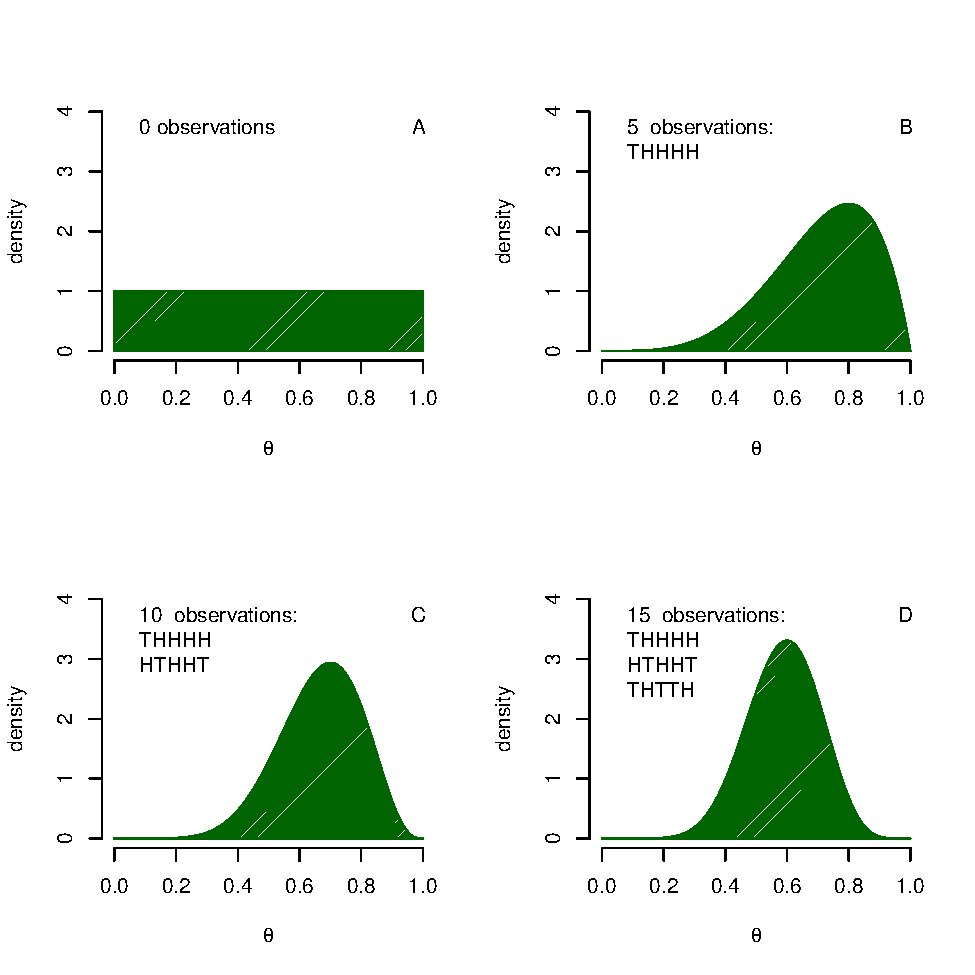
\includegraphics{Dissertation_Duco_Veen_files/figure-latex/binomUninformative-1} 

}

\caption{Example of Bayesian updating. Panel A shows a $Beta(\alpha = 1, \beta = 1)$ distribution representing a prior state of knowledge equal to ignorance. Panels B, C and D show how the state of knowledge updated after new data is observed, each time the previous panel is the prior belief for the next panel, combined with the information from five new observations.}\label{fig:binomUninformative}
\end{figure}

Now, let us suppose that we did not have an initial state of ignorance. The \emph{prior} need not be ignorance as we noticed when the previous posterior became our new prior each time. Would of belief differ if we had more initial information? Figure \ref{fig:binomInf} shows learning from the same data as in the example presented in Figure \ref{fig:binomUninformative} with our initial state of knowledge expressed by a \(Beta(\alpha = 51, \beta = 51)\) distribution. In other words, before the new trials we had initial information equivalent to 100 previous coin flips that were distributed equally between head and tails. The new data is very much in line with our previous data and we only slightly adjust our beliefs, assigning even more probability to values near .5.

\begin{figure}

{\centering 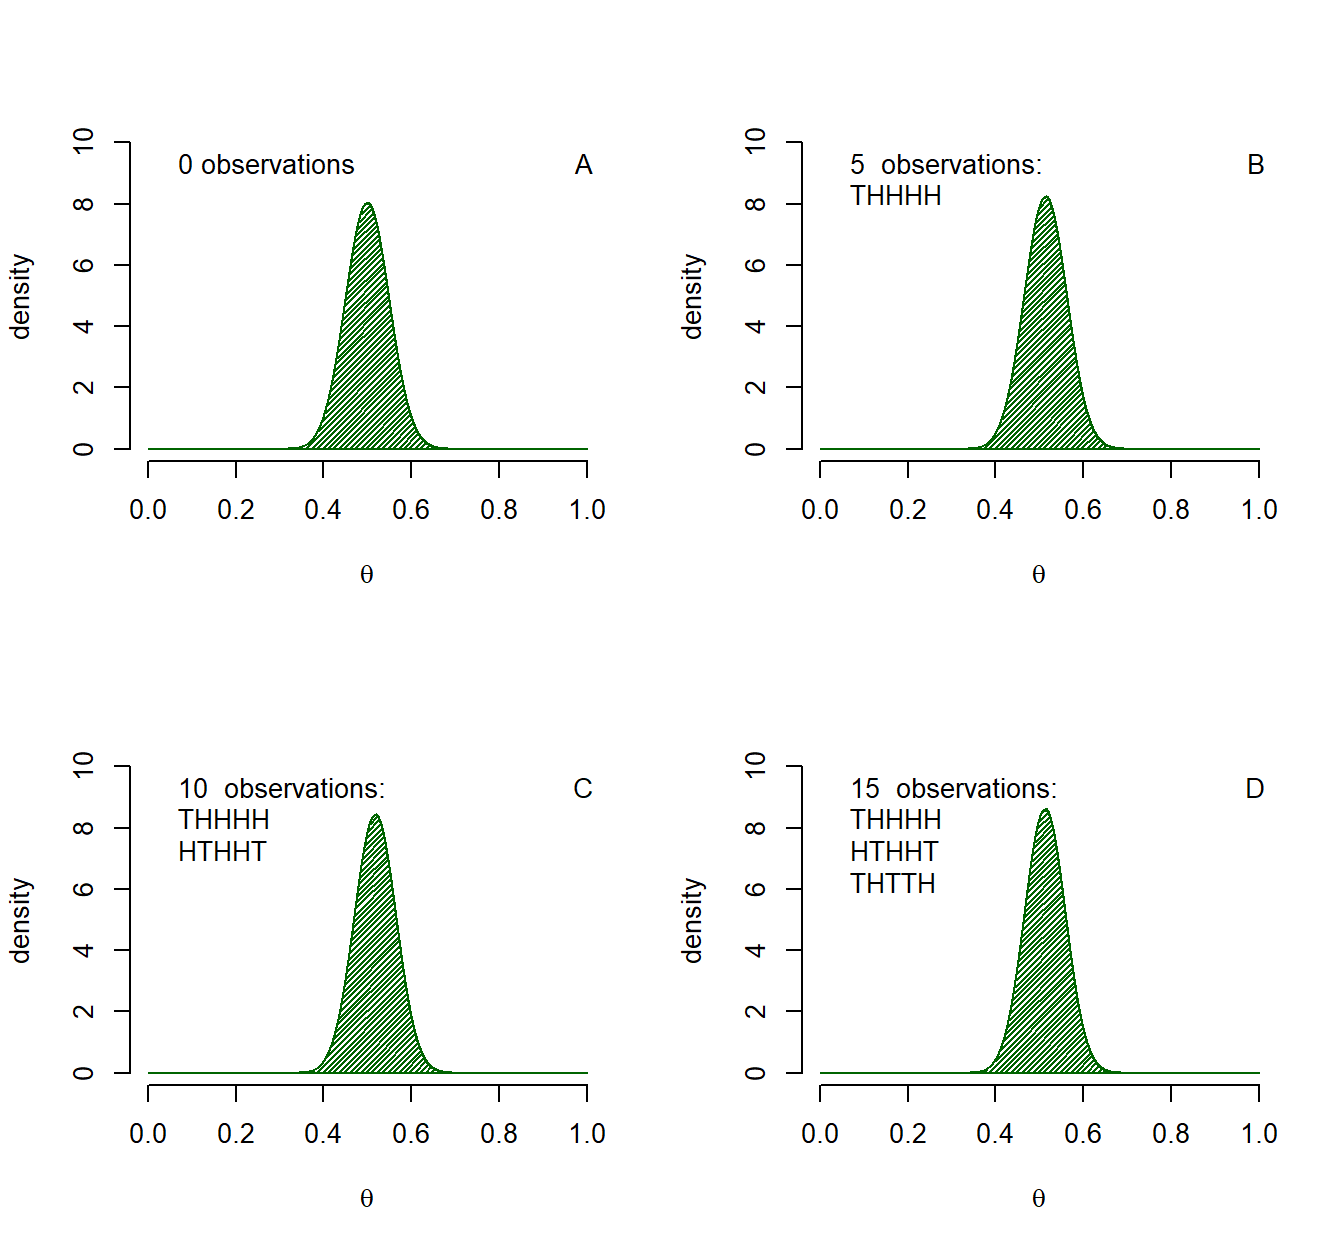
\includegraphics{Dissertation_Duco_Veen_files/figure-latex/binomInf-1} 

}

\caption{Example of Bayesian updating. Panel A shows a $Beta(\alpha = 51, \beta = 51)$ distribution. This is updated using the same data as in Figure 1.1, only the initial prior contains more information.}\label{fig:binomInf}
\end{figure}

All of this wonderful nuanced theory is historically summarized by a single equation. The reason for showing you this formula only after the examples, is not to get distracted by the mathematics for those readers not working with statistics every day. For those who do use statistics often, there are many books written in much more detail on this subject that yield a more complete overview (e.g.~Gelman et al., \protect\hyperlink{ref-gelman_bayesian_2013}{2013}; Jaynes, \protect\hyperlink{ref-jaynes_probability_2003}{2003}; Kaplan, \protect\hyperlink{ref-kaplan_bayesian_2014}{2014}; Lindley, \protect\hyperlink{ref-lindley_understanding_2013}{2013}; Lynch, \protect\hyperlink{ref-lynch_introduction_2007}{2007}; Ntzoufras, \protect\hyperlink{ref-ntzoufras_bayesian_2011}{2011}; Press, \protect\hyperlink{ref-press_subjective_2009}{2009}). Without further ado, Bayes' Theorem

\begin{equation} 
p(A|BC) = P(A|C)\frac{P(B|AC)}{P(B|C)}
\label{eq:bayestheorem}
\end{equation}

where \(A\), \(B\) and \(C\) are different propositions, \(p(A|C)\) describes the \emph{prior} distribution of probability concerning \(A\), given that we know \(C\). \(p(A|BC)\) is the \emph{posterior} distribution of probability concerning \(A\), updated with the new information that is provided to us by \(B\). Note that \(C\) here has the interpretation of what we know about \(A\) before learning about, or obtaining, the information from \(B\). In the previous example, \(\theta\) took on the role of \(A\) and the new trials took on the role of \(B\). \(C\), in the first example, expressed that we knew that \(\theta\) was a proportion which can only take on values in the interval from 0 up to 1. Equation \eqref{eq:bayestheorem} describes how we can learn about \(A\), how we ought to update our beliefs in the light of new data. It also makes it explicit that this learning effect is dependent on our prior knowledge, just like in the example of Figures \ref{fig:binomUninformative} and \ref{fig:binomInf} Again, the aim here is not to expand on the mathematics, but merely to provide some initial intuition about the concept of learning using Bayes' rule. Next, we turn to the implementation of the concept of prior knowledge, how can we formalize our prior distribution of probability concerning \(A\) given that we know \(C\).

\hypertarget{prior-information}{%
\section{Prior Information}\label{prior-information}}

The topic of prior information in Bayesian statistics is a field of study all on it's own. To illustrate this, note that Tuyl, Gerlach, \& Mengersen (\protect\hyperlink{ref-tuyl_comparison_2008}{2008}) wrote a full paper, discussing only the choice of prior for extreme cases of our example above. There are heavy discussions and different schools of thought, roughly divided into ``objective'' (e.g.~Berger, \protect\hyperlink{ref-berger_case_2006}{2006}) and ``subjective'' (e.g.~Finetti, \protect\hyperlink{ref-de_finetti_theory_1974}{1974}; Goldstein, \protect\hyperlink{ref-goldstein_subjective_2006}{2006}) camps. Discussing the differences within, let alone between, these different approaches is way to much to get into at this point. Simply listing names of different approaches to objective Bayesian priors takes up an extensive paragraph (Berger, \protect\hyperlink{ref-berger_case_2006}{2006}, pp. 387--388) and for a discussion about the (dis)advantages of both method I refer the reader to Chapter 5 of Press (\protect\hyperlink{ref-press_subjective_2009}{2009}). For the reader it suffices to know that in this dissertation we certainly specify priors that would be considered more in line with the ``subjective'' school of Bayesian analysis, even if we do not always use these priors to be updated with new data.

Now let us briefly consider three types of information that could be included in a prior distribution of probability. First, previous research can inform us about certain parameters and including this information in future analyses seems in line with our idea of leaning. In Section 5.4 of Spiegelhalter, Abrams, \& Myles (\protect\hyperlink{ref-spiegelhalter_bayesian_2004}{2004}) they provide a very nice overview on how to include results of previous studies based on similarity, exchangability and bias considerations. It is described not only how you could include information from previous studies if they are exactly on the same topic, but also how to do so if the research differs in specific ways. Second, logical considerations can be taken into account, e.g.~in the coin flipping example we know that a proportion lies between 0 and 1 and no values outside the interval between those two will be assigned any probability. In a similar fashion we could incorporate information with respect to our measurements, e.g.~no negative values for temperature measured in Kelvin, or when calculating air pollution in a city that we do live in, the amount of matter in the air cannot be so much that we could not breath and live there. Third,
information gathered from an expert, or as put by the Dictionary (\protect\hyperlink{ref-cambridge_english_dictionary_expert_2019}{2019}); ``\emph{a person with a high level of knowledge or skill relating to a particular subject or activity}''. This particular knowledge can be translated, or elicited, to be expressed in the form of distribution of probability. There are surely more sources of information to inform our prior probability distributions besides previous research, logical considerations and expert knowledge, but as this dissertations involves experts quite a bit I will elaborate on that specific case somewhat more.

\hypertarget{expert-elicitation}{%
\section{Expert Elicitation}\label{expert-elicitation}}

The process of creating a probabilistic representation of an experts' beliefs is called elicitation (O'Hagan et al., \protect\hyperlink{ref-ohagan_uncertain_2006}{2006}). There is an extensive history of expert elicitation across many different disciplines of sciences (Cooke \& Goossens, \protect\hyperlink{ref-cooke_tu_2008}{2008}; Gosling, \protect\hyperlink{ref-gosling_shelf:_2018}{2018}; O'Hagan et al., \protect\hyperlink{ref-ohagan_uncertain_2006}{2006}, Chapter 10). Expert judgements are for instance used in the case that there is no actual data available (Hald et al., \protect\hyperlink{ref-hald_world_2016}{2016}) or to add information to small sample data (Kadane, \protect\hyperlink{ref-kadane_application_1994}{1994}). However, with many examples, covering many disciplines, expert knowledge still does not seem to be used in the social sciences with Van de Schoot, Winter, Ryan, Zondervan-Zwijnenburg, \& Depaoli (\protect\hyperlink{ref-van_de_schoot_systematic_2017}{2017}) finding only two use cases in the past 25 years of Bayesian statistics in Psychology.

One of the reasons for this limited use can perhaps be found in the traditional way of eliciting expert judgements. One of the traditional ways is to elicit three quantiles from an experts concerning the distribution of probability over a specific parameters (O'Hagan et al., \protect\hyperlink{ref-ohagan_uncertain_2006}{2006}, Chapter 5). These quantiles are then used to determine the distribution that fits best with these described value, and that distribution is used to represent an experts' beliefs. The questions to the experts would be for instance the following:

\begin{quote}
"Q1: Can you determine a value (your median) such that X is equally likely to be less than or greater than this point?

Q2: Suppose you were told that X is below your assessed median. Can you now determine a new value (the lower quartile) such that it is equally likely that X is less than or greater than this value?

Q3: Suppose you were told that X is above your assessed median. Can you now determine a new value (the lower quartile) such that it is equally likely that X is less than or greater than this value?"

O'Hagan et al. (\protect\hyperlink{ref-ohagan_uncertain_2006}{2006}), p.~101
\end{quote}

We believe that this rather abstract thinking in terms of quantiles of distributions might be hard for some experts, depending on their experience with statistics and mathematical background. This naturally bring us to the following section and the outline of this dissertation, how is it that we propose to use expert elicitation in the social sciences and what do we propose to do with this source of additional information.

\hypertarget{aims-and-outline}{%
\section{Aims and Outline}\label{aims-and-outline}}

In this dissertation it is discussed how one can capture and utilize alternative sources of (prior) information compared to traditional method in the social sciences such as survey research. Specific attention is paid to expert knowledge.

In Chapter \protect\hyperlink{fivestep}{2} we propose an elicitation methodology for a single parameter that does not rely on specifying quantiles of a distribution. The proposed method is evaluated using a user feasibility study, a partial validation study and an empirical example of the full elicitation method.

In Chapter \protect\hyperlink{DAC1}{3} it is investigated how experts' knowledge, as alternative source of information, can be contrasted with traditional data collection methods. At the same time, we explore how experts can be assessed and ranked borrowing techniques from information theory. We use the information theoretical concept of relative entropy or Kullback-Leibler divergence which assesses a loss of information when approximating one distribution by another. For those familiar with the concept of model selection, Akaike's Information Criterion is an approximation of this (Burnham \& Anderson, \protect\hyperlink{ref-burnham_model_2002}{2002}, Chapter 2).

In Chapter \protect\hyperlink{Hierarchical}{4} an alternative way of enhancing the amount of information in a model is proposed. We introduce Bayesian hierarchical modelling to the field of infants' speech discrimination analysis. This technique is not new on it's own but was not applied to this field. Implementing this type of modelling enables individual analyses within a group structure. By taking the hierarchical structure of the data into account we can make the most of the, on individual level, small noisy data sets. The analysis methodology estimates if individuals are (dis)similar and takes this into account for all individuals in one single model. Essentially, the estimated group effects serve as priors for the individual estimates. Moreover, we do not need to do a single hypothesis test for every child, which was the most advanced individual analysis in the field up to now, going back to 2007 (Houston, Horn, Qi, Ting, \& Gao, \protect\hyperlink{ref-houston_assessing_2007}{2007}).

In Chapter \protect\hyperlink{Burns}{5} we reflect on issues that come along with the estimation of increasingly complicated models. Techniques and software for estimating more complex models, such as proposed in Chapter \protect\hyperlink{Hierarchical}{4}, need to be carefully used and the results of the analyses need to be carefully checked. But what to do when things actually go awry in your analysis? We show how even with weakly informative priors, adding the information that is available to us, sometimes we do not get a solution with our analysis plan. We guide the reader on what to do when this occurs and where to look for clues and possible causes. We provide some guidance and a textbook example that for once shows things not working out the way you would like. We believe this is important as there are few examples of this.

In Chapter \protect\hyperlink{elicitlgm}{6} we combine the previous chapters. We take more complex models and get experts to specify beliefs with respect to these models. We extend the method developed in Chapter \protect\hyperlink{fivestep}{2} to elicit experts' beliefs with respect to a hierarchical model, which is used in Chapters \protect\hyperlink{Hierarchical}{4} and \protect\hyperlink{Burns}{5}. In specific, we concern ourselves with a Latent Growth Curve model and utilize the information theoretical measures from Chapter \protect\hyperlink{DAC1}{3} to compare the (groups) of experts to one another and to data collected in a traditional way. We do this in the context of Posttraumatic Stress Symptoms development in children with burn injuries.

In Chapter \protect\hyperlink{thesisdiscussion}{7} I reflect on the work and explanations provided within the chapters of this dissertation, including this introduction. The discussion is a reflection of my own personal thoughts, and no other person is responsible for the content, although the personal discussions and collaborations of the past years have certainly contributed to the formulation of these opinions.

\hypertarget{fivestep}{%
\chapter{Proposal for a Five-Step Method to Elicit Expert Judgment}\label{fivestep}}

\chaptermark{FIVE-STEP METHOD}
\thispagestyle{empty}

\blfootnote{This chapter is published as Veen, D., Stoel ,D., Zondervan-Zwijnenburg, M. \& van de Schoot, R. (2017). Proposal for a Five-Step Method to Elicit Expert Judgment. \textit{Front. Psychol.}, 8:2110. doi: 10.3389/fpsyg.2017.02110 \\ \indent DV and RvdS mainly contributed to the study design. All authors have been involved in the design of (part) of the elicitation procedure. DV programmed the elicitation software. All elicitations have been facilitated by DV and DS. DV wrote and revised the paper with feedback and input of DS, MZ-Z, and RvdS. RvdS supervised the project.}

\hypertarget{abstract}{%
\section*{Abstract}\label{abstract}}
\addcontentsline{toc}{section}{Abstract}

\small

Elicitation is a commonly used tool to extract viable information from experts. The information that is held by the expert is extracted and a probabilistic representation of this knowledge is constructed. A promising avenue in psychological research is to incorporated experts' prior knowledge in the statistical analysis. Systematic reviews on elicitation literature however suggest that it might be inappropriate to directly obtain distributional representations from experts. The literature qualifies experts' performance on estimating elements of a distribution as unsatisfactory, thus reliably specifying the essential elements of the parameters of interest in one elicitation step seems implausible. Providing feedback within the elicitation process can enhance the quality of the elicitation and interactive software can be used to facilitate the feedback. Therefore, we propose to decompose the elicitation procedure into smaller steps with adjustable outcomes. We represent the tacit knowledge of experts as a location parameter and their uncertainty concerning this knowledge by a scale and shape parameter. Using a feedback procedure, experts can accept the representation of their beliefs or adjust their input. We propose a Five-Step Method which consists of (1) Eliciting the location parameter using the trial roulette method. (2) Provide feedback on the location parameter and ask for confirmation or adjustment. (3) Elicit the scale and shape parameter. (4) Provide feedback on the scale and shape parameter and ask for confirmation or adjustment. (5) Use the elicited and calibrated probability distribution in a statistical analysis and update it with data or to compute a prior-data conflict within a Bayesian framework. User feasibility and internal validity for the Five-Step Method are investigated using three elicitation studies.

\normalsize
\newpage

\hypertarget{ch02introduction}{%
\section{Introduction}\label{ch02introduction}}

\begin{quote}
``The knowledge held by expert practitioners is too valuable to be ignored. But only when thorough methods are applied, can the application of expert knowledge be as valid as the use of empirical data. The responsibility for the effective and rigorous use of expert knowledge lies with the researchers.''

Drescher et al. (\protect\hyperlink{ref-drescher_toward_2013}{2013}, p. 1)
\end{quote}

According to O'Hagan et al. (\protect\hyperlink{ref-ohagan_uncertain_2006}{2006}) elicitation is the process of extracting and creating a representation of an expert's beliefs. It can be used for a variety of reasons, e.g., to add information to small sample data (Kadane, \protect\hyperlink{ref-kadane_application_1994}{1994}; Schoot, Sijbrandij, et al., \protect\hyperlink{ref-van_de_schoot_bayesian_2018}{2018}; Zondervan-Zwijnenburg et al., \protect\hyperlink{ref-zondervan-zwijnenburg_where_2017}{2017}\protect\hyperlink{ref-zondervan-zwijnenburg_where_2017}{a}), when there is no data for certain confounding parameters in a model (Fischer, Lewandowski, \& Janssen, \protect\hyperlink{ref-fischer_estimating_2013}{2013}), when no data is available (Ho \& Smith, \protect\hyperlink{ref-ho_volcanic_1997}{1997}), as sensitivity analysis to check assumptions about missing data (Mason et al., \protect\hyperlink{ref-mason_development_2017}{2017}), or simply to enrich the available data (Wisniowski, Bijak, \& Shang, \protect\hyperlink{ref-wisniowski_forecasting_2014}{2014}). Expert knowledge is a valuable source of information, as becomes evident in the quote of Drescher et al. (\protect\hyperlink{ref-drescher_toward_2013}{2013}). (Hadorn, Kvizhinadze, Collinson, \& Blakely, \protect\hyperlink{ref-hadorn_useof_2014}{2014}) found that 57\% of health economic decision models included at least one expert knowledge elicitation parameter, showing that in some fields it is even the norm to use expert elicitation. More examples of elicitation practices in many different fields can be found in overview studies by O'Hagan et al. (\protect\hyperlink{ref-ohagan_uncertain_2006}{2006}, Chapter 10) and Bistline (\protect\hyperlink{ref-bistline_energy_2014}{2014}) or the paper by Cooke \& Goossens (\protect\hyperlink{ref-cooke_tu_2008}{2008}) in which they describe the data base of over 67,000 experts' subjective probability distributions.

There are many elicitation procedures available, overviews can be found in for instance O'Hagan et al. (\protect\hyperlink{ref-ohagan_uncertain_2006}{2006}), S. R. Johnson et al. (\protect\hyperlink{ref-johnson_methods_2010}{2010}), and Aspinall \& Cooke (\protect\hyperlink{ref-aspinall_quantifying_2013}{2013}). A popular elicitation method is the trial roulette method (Gore, \protect\hyperlink{ref-gore_biostatistics_1987}{1987}), sometimes also called the chips and bins method or the histogram method, in which experts assign ``chips''" to ``bins'' of a histogram to ascribe probability. In the procedure, used by for instance Diamond et al. (\protect\hyperlink{ref-diamond_expert_2014}{2014}) and Goldstein \& Rothschild (\protect\hyperlink{ref-goldstein_lay_2014}{2014}), the parameter space for which experts can assign probability is divided into equal sections or ``bins''. The experts receive 20 ``chips'', which are to be distributed amongst these ``bins''. For each ``chip'' that is allocated to one of the ``bins'', 5\% of the mass of a probability distribution is ascribed. Based on the input provided by the expert, a probability distribution is fitted. The trial roulette method has been validated by S. R. Johnson, Tomlinson, et al. (\protect\hyperlink{ref-johnson_valid_2010}{2010}) and M. Zondervan-Zwijnenburg et al. (\protect\hyperlink{ref-zondervan-zwijnenburg_application_2017}{2017}\protect\hyperlink{ref-zondervan-zwijnenburg_application_2017}{b}) in a face-to-face setting.

Software that can be used in the elicitation with the trial roulette method is available in the MATCH Uncertainty Elicitation Tool (Morris, Oakley, \& Crowe, \protect\hyperlink{ref-morris_web-based_2014}{2014}). MATCH is an online framework for elicitation procedures. It uses the R-package (R Core Team, \protect\hyperlink{ref-r_core_team_r:_2017}{2017}\protect\hyperlink{ref-r_core_team_r:_2017}{b}) SHELF (Oakley, \protect\hyperlink{ref-R-SHELF}{2019}) to fit appropriate parametric distributions based on input that is provided by experts.

One of the reasons the trial roulette method is popular is that the procedure provides immediate visual feedback to experts. Feedback is important in elicitation procedures to reduce bias and improve the quality of the elicitation (Johnson et al., \protect\hyperlink{ref-johnson_methods_2010}{2010}; O'Hagan et al., \protect\hyperlink{ref-ohagan_uncertain_2006}{2006}). The ``chips''" that are allocated in the trial roulette method by the expert visually approximate a probability distribution. However, the feedback provided to the expert is not on the statistical distribution that is actually used by the researcher in the final analyses. It is important to receive conformation of the expert that the interpretation by the researcher matches their beliefs, or as O'Hagan et al. (\protect\hyperlink{ref-ohagan_uncertain_2006}{2006}, p. 174) state, \emph{``feedback to the expert is the most natural way of evaluating the distribution -- the expert is in the best position to judge whether something corresponds to her opinion.''} Providing instant feedback on the representation of the experts' beliefs, based on the input they provide, and how their beliefs are translated into a statistical distribution can easily be done by using software.

Feedback is believed to improve the quality of the elicitation procedure by making experts; reflect and maintain selfconsistency (Fisher, O'Leary, Low-Choy, Mengersen, \& Caley, \protect\hyperlink{ref-fisher_software_2012}{2012}), by highlighting inconsistencies in judgment and making errors apparent (Morris et al., \protect\hyperlink{ref-morris_web-based_2014}{2014}; O'Hagan et al., \protect\hyperlink{ref-ohagan_uncertain_2006}{2006}) and by allowing for self-correction by experts (Johnson et al., \protect\hyperlink{ref-johnson_methods_2010}{2010}). Despite assumed quality improvement by feedback, systematic reviews on elicitation literature by O'Hagan et al. (\protect\hyperlink{ref-ohagan_uncertain_2006}{2006}) and Johnson et al. (\protect\hyperlink{ref-johnson_methods_2010}{2010}) conclude that measurement properties of elicitation methods have not been adequately evaluated. Moreover, there is no direct research into how accurate experts can assess properties like the mean, mode, or variance for the distribution of an uncertain parameter. Research by S. R. Johnson, Tomlinson, et al. (\protect\hyperlink{ref-johnson_valid_2010}{2010}) and (Zondervan-Zwijnenburg et al., \protect\hyperlink{ref-zondervan-zwijnenburg_application_2017}{2017}\protect\hyperlink{ref-zondervan-zwijnenburg_application_2017}{b}) provide promising results concerning the trial roulette method. Yet, directly obtaining distributional representations may be inappropriate given experts' unsatisfactory performance on specifying elements of this distribution. O'Hagan et al. (\protect\hyperlink{ref-ohagan_uncertain_2006}{2006}) refer to research by Hofstatter (\protect\hyperlink{ref-hofstatter_uber_1939}{1939}), Lathrop (\protect\hyperlink{ref-lathrop_perceived_1967}{1967}) and, Beach \& Scopp (\protect\hyperlink{ref-beach_intuitive_1968}{1968}) to show that experts are not good at interpreting and assigning numerical values to variances and relative variability. It might then be unreasonable to assume that experts are able to reliably specifying a probability distribution in one step.

Therefore, to assist experts in the process of creating a representation of their beliefs in a statistical distribution we propose to decompose the elicitation task in smaller steps to encourage and assist in structured reasoning. Decomposing a problem into more tractable and familiar components is suggested by for instance Fischhoff (\protect\hyperlink{ref-fischhoff_debiasing_1982}{1982}) to decrease the mismatch between the judge and the task. By decomposing the elicitation task we aim to reduce bias and incorporate more feedback to ensure that experts' opinions are properly calibrated and represented by the probability distributions that results from the elicitation. In the current paper, the statistical distribution of interest is the skewed normal (SN) distribution\footnote{Using the SN distribution we represent the tacit knowledge of experts by eliciting the location parameter of the distribution, in this case the mean. The uncertainty of the expert about his/her belief on the location parameter is represented by the scale and shape parameter (i.e., variance and skewness of the normal distribution). Eliciting the mean of a normal distribution offers the advantage of easily transformable scale for elicitation procedures. An adjustable scale means that even if one expert reasons in averages and the other expert in sums they can be transformed to be comparable, i.e., let \(\theta\) represent the parameter of interest and \(\theta \sim N(\mu, \sigma^2)\) and if we transform \(\theta\) via the following function \(\theta^* = a\theta+b\), then \(\theta^* \sim N[a\mu+b,(a\sigma)^2]\).} because uncertainty might typically not best be captured by a symmetric distribution. This (un)certainty is the key feature of Bayesian statistics, uncertainty reveals the extent of our knowledge and ignorance (Finetti, \protect\hyperlink{ref-de_finetti_theory_1974}{1974}).

We propose the Five-Step Method which consists out of the following steps:

\begin{enumerate}
\def\labelenumi{\arabic{enumi}.}
\tightlist
\item
  Elicit the location parameter of the SN using the trial roulette method.
\item
  Use software to provide instant feedback on the interpretation of the expert's beliefs by the researcher so the expert can accept this representation or adjust their input.
\item
  Elicit the (un)certainty of the expert by determining the scale and shape parameters of the SN using expert's statements on the lower and upper bounds for a plausible range of the parameter values.
\item
  Use software to provide instant feedback on the interpretation of the expert's (un)certainty about the location parameter by the researcher so expert can accept this representation or adjust their input.
\item
  Use the elicited and calibrated probability distribution in a Bayesian analysis to update it with data or to compute a prior-data conflict.
\end{enumerate}

The remainder of the paper is ordered as follows. We first provide details on the Five-Step Method. Thereafter we present a user feasibility study in which we elicited beliefs regarding a trivial sports related question from respondents to investigate visual and procedural preferences of users for the digitized version of the trial roulette method. A second study was carried out by asking experts working at a staffing company about certain key performance indicators which we used to validate the internal validity of steps 1 and 2 of the elicitation procedure. A final study was done with regional directors working at a large financial institution. They provided actual forecasts concerning average turnover per professional in the first quarter of the year 2016 with the Five-Step Method. The participating companies already make predictions concerning the parameters we elicit, yet they do this in the form of point estimates. The experts are thus already used to thinking about these data and predicting these data which makes them highly suitable to include as experts in an elicitation exercise. Yet, it is an extension for them to actively specify and separate knowledge and uncertainty. Because the companies also provided us with data on the predicted parameters we were able to compare the forecasts of the experts with data and thereby get an indication of the internal validity of the elicitation procedure. The proposition to split the elicitation process results in a procedure differing from the existing elicitation procedures as, for example, proposed by Oakley (\protect\hyperlink{ref-oakley_eliciting_2010}{2010}), or that can be carried out through the use of existing software like MATCH. Therefore, we programmed our own software. All related materials for this study, including code and data, can be found on the Open Science Framework (OSF) webpage at \url{https://osf.io/wvujz}.

\hypertarget{five-step-method}{%
\section{Five-Step Method}\label{five-step-method}}

In this section we describe the technical details of the Five-Step Method which has been programmed in R (R Core Team, \protect\hyperlink{ref-r_core_team_r:_2017}{2017}\protect\hyperlink{ref-r_core_team_r:_2017}{b}) using the shiny package (Chang, Cheng, Allaire, Xie, \& McPherson, \protect\hyperlink{ref-R-shiny}{2019}).

\hypertarget{step-1}{%
\subsection{Step 1}\label{step-1}}

The first step of the Five-Step Method consists of a digitized version of the trial roulette, which can be seen in Figure \ref{fig:ch02fig1}. Instead of vertical ``bins'' a grid is used and the digital ``chips'' can be placed on the grid. Experts provide estimates for the expected minimum and maximum value of the parameter of interest, represented by the left and rightmost digital ``chips'' in the grid, based on which the range of the grid is determined. Thereafter they place additional ``chips'' in the grid. In specific, the input grid, denoted by \textbf{G}, is a matrix size 600 (columns) x 300 (rows) and cells are activated by the placement of a digital ``chips'' in the grid. The cells where a sticker is placed obtain a value of one, all other cells are set to non-available. A second matrix, denoted by \textbf{R} of the same dimensions is created in which all rows are equal and the columns are a sequence of numbers with equal intervals running from the reasonable lower to upper bound provided as input. We then create output matrix \textbf{O} which contains values from \textbf{R} activated by the placement of dots in \textbf{G} and after the deletion of all nonavailable values in \textbf{O}, the remaining values are stored in a vector.

\begin{figure}

{\centering 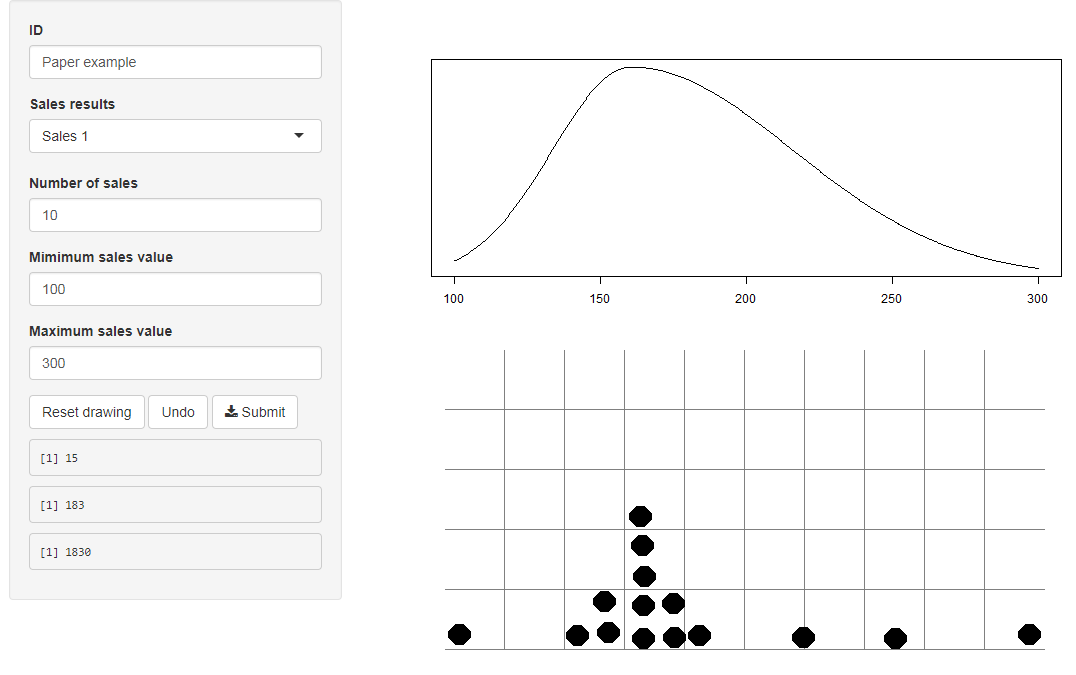
\includegraphics[width=0.85\linewidth]{figures/chapter_2/Figure_1} 

}

\caption{Shiny application for steps 1 and 2. On the left the input fields can be found for the reasonable lower and upper bound as minimum and maximum values. The input grid in which 'chips' can be  placed is found on the lower right with the leftmost dot being the minimum value and the right most dot being the maximum value. Further 'chips' are placed by clicking the mouse drawing a maximum of 11 pixels left and right. On the top right feedback is provided, presenting the fitted distribution based on the input.}\label{fig:ch02fig1}
\end{figure}

\hypertarget{step-2}{%
\subsection{Step 2}\label{step-2}}

The vector of values that is elicited in step 1 are used to fit a SN distribution. The SN distribution is defined in this paper as a normal distribution with the additional shape parameter \(\gamma\). The shape parameter is based upon a general method for the transformation of symmetric distributions into skewed distributions as described in Fernández \& Steel (\protect\hyperlink{ref-fernandez_bayesian_1998}{1998}). The transformation of the symmetric distribution into a skewed distribution is done by allocating mass of the distribution to either side of the mode (\emph{M}) by controlling the error term (\(\epsilon\)) via the following function, taken from Fernandez and Steel Eq. 1:

\begin{equation} 
p(\epsilon|\gamma) = \frac{2}{{\gamma + \frac{1}{\gamma}}} {f(\frac{\epsilon}{\gamma})I_{(M,\infty)}(\epsilon) + f(\gamma \epsilon)I_{(-\infty,M)}(\epsilon)}.
\label{eq:ch02eq1}
\end{equation}

The effect of the shape parameter on the allocation of mass can be seen in Figure \ref{fig:ch02fig2}. Note that the distributions would be exactly mirrored with respect to the mode if the \(\gamma\) values would be \(\frac{1}{\gamma}\).

To fit the SN distribution we make use of the snormFit function from the fGarch package (Wuertz et al., \protect\hyperlink{ref-R-fGarch}{2019}). This function uses an optimization algorithm to determine the optimal skewness parameter based on log-likelihood values. The mean and standard deviation are determined based on the vector of elicited values. The mean and standard deviation remain constant and thus there is only one parameter to optimize over, the shape parameter \(\gamma\).

The SN distribution that is fitted based upon the expert's input is provided as visual feedback to the expert, see Figure \ref{fig:ch02fig1}. The visual feedback indicates how we interpret the information that is provided by the expert. The expert can accept the representation of their beliefs or adjust input until the representation matches their beliefs. Once the expert approves the representation of their beliefs, the mean value is extracted from the distribution which is to be used in step 3.

\begin{figure}

{\centering 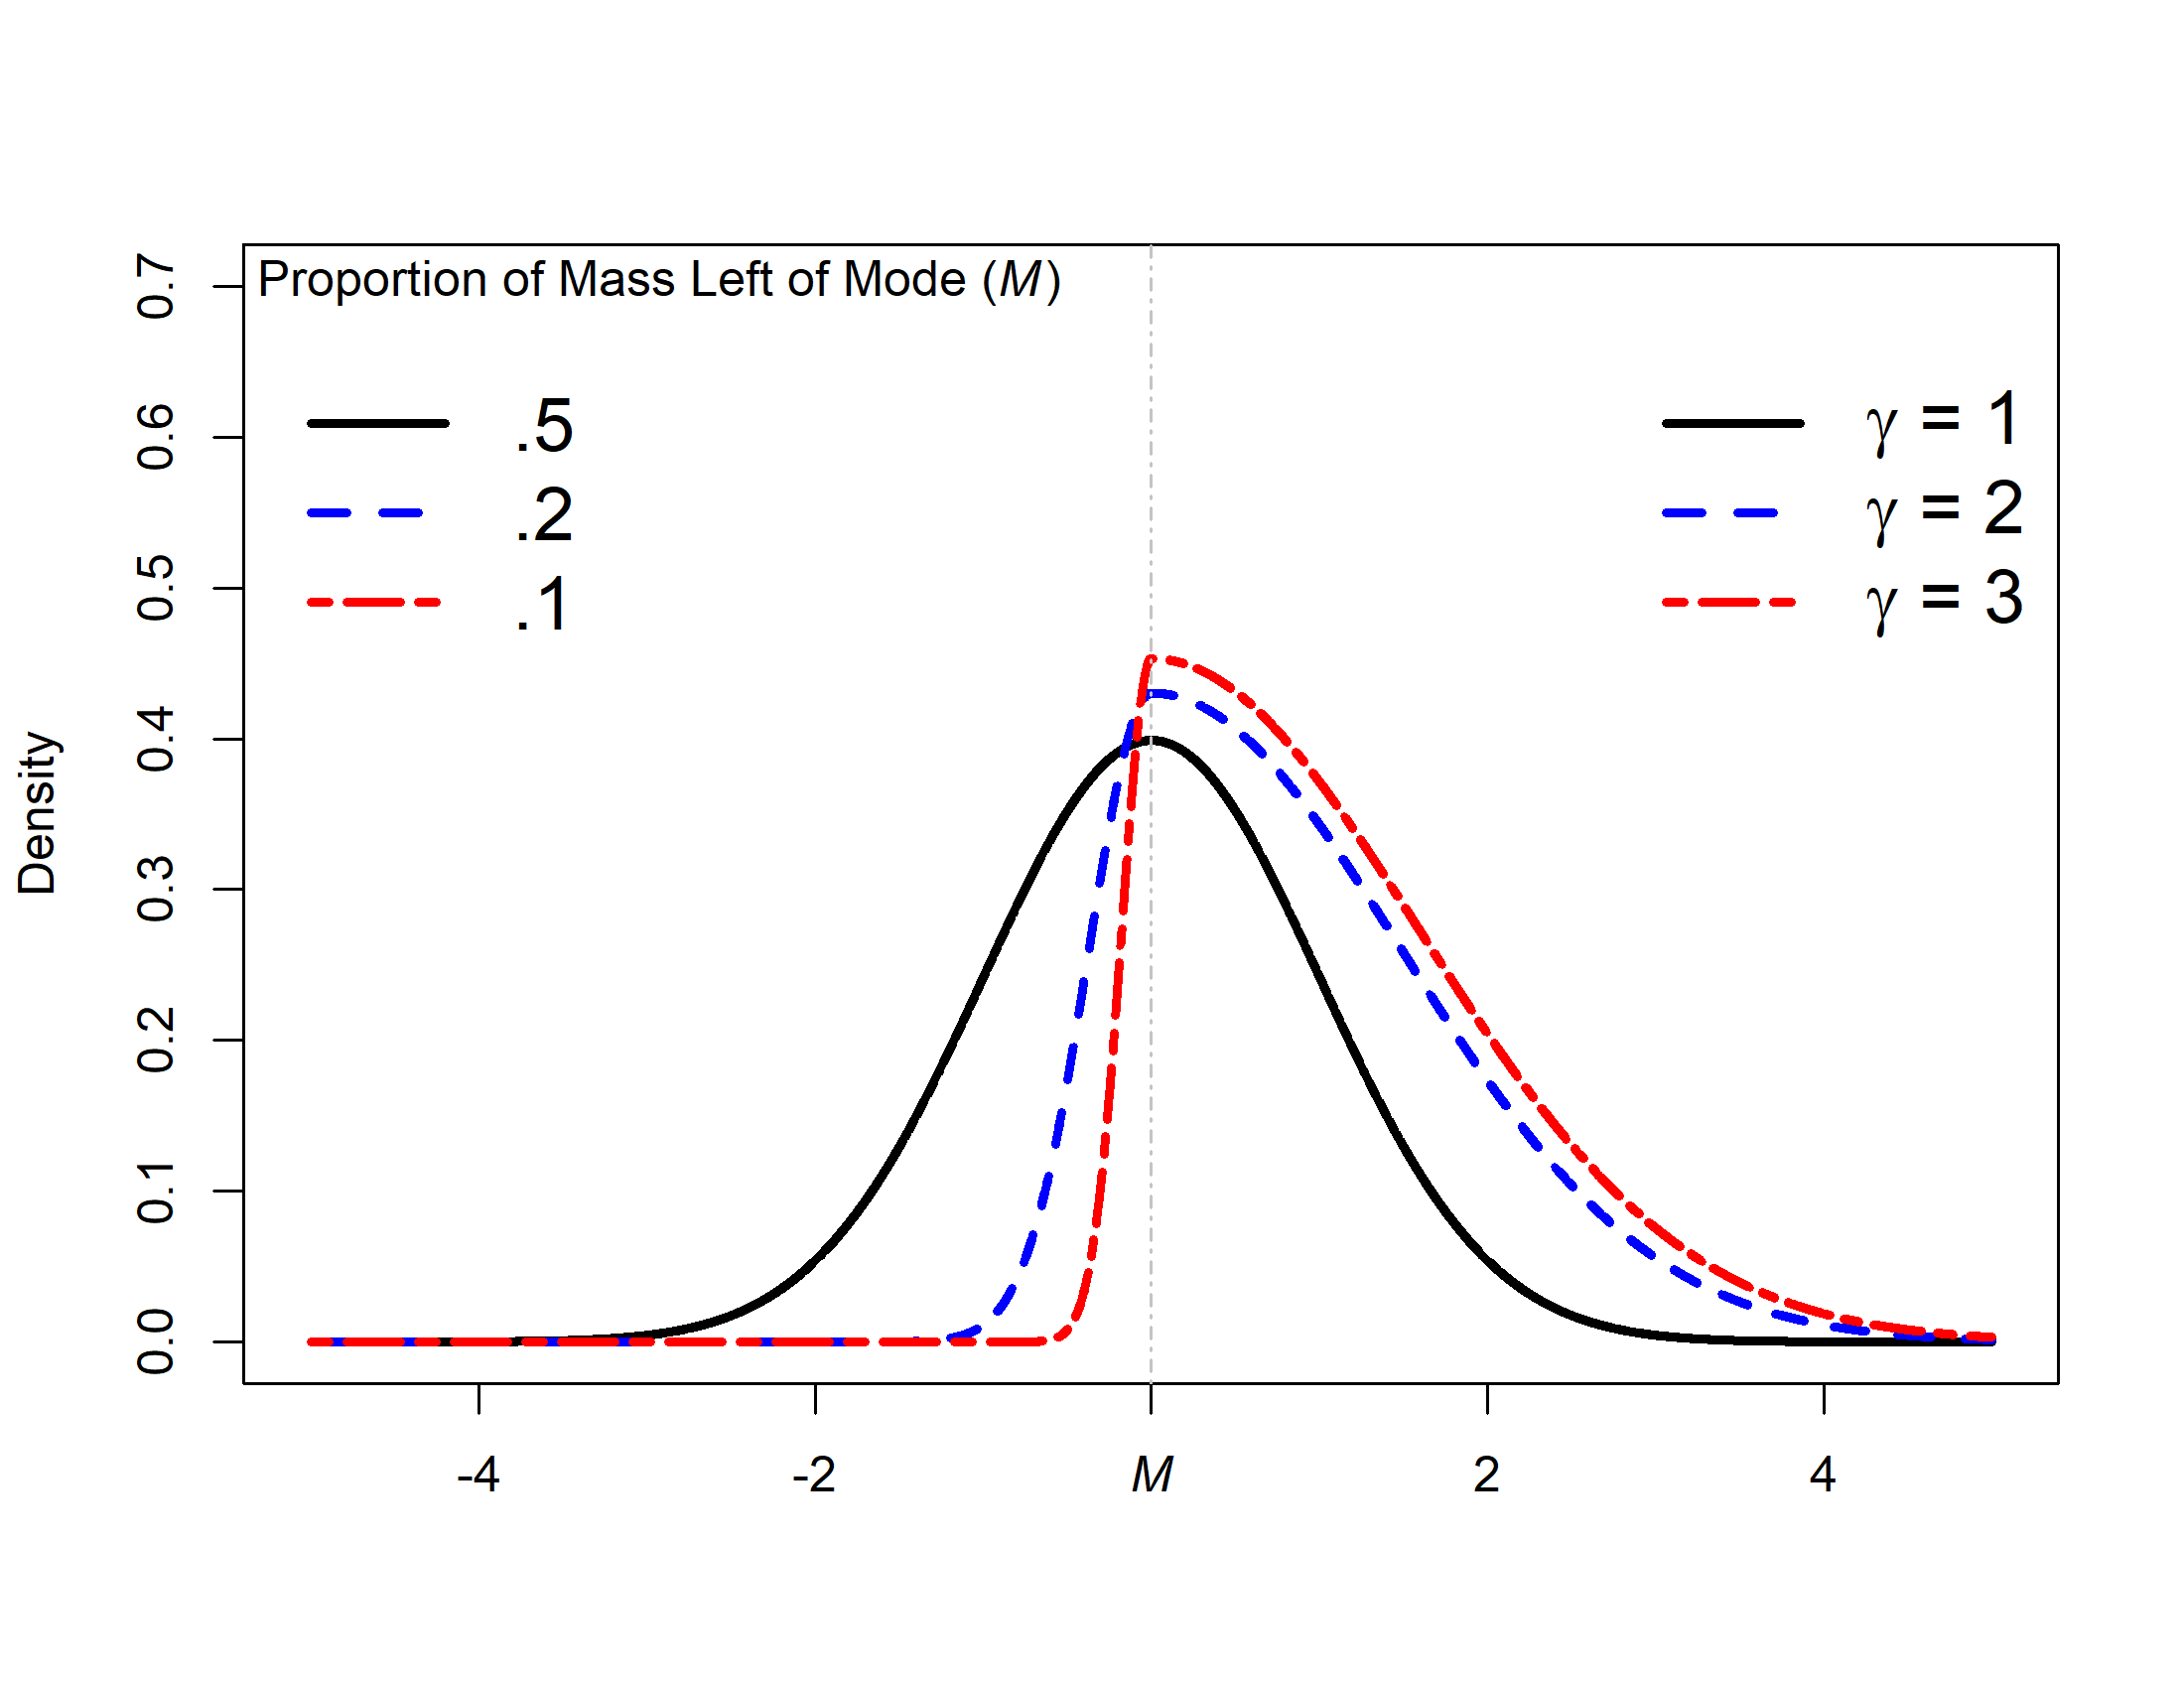
\includegraphics[width=0.85\linewidth]{figures/chapter_2/Figure_2} 

}

\caption{Example of the influence of shape parameter $\gamma$ on the allocation of mass for a normal distribution with a variance of 1.}\label{fig:ch02fig2}
\end{figure}

\hypertarget{step-3}{%
\subsection{Step 3}\label{step-3}}

Step 3 of the Five-Step Method is used to derive the distributional representation of the expert's prior beliefs concerning the parameter of interest and can be seen in Figure \ref{fig:ch02fig3}. We restricted the priors that represent the experts' beliefs to be SN distributions so \(\pi_d \sim SN(\mu_0, \sigma^2_0, \gamma_0)\), where subscript \emph{d} denotes expert \(d = 1,...,D\), \(\mu_0\) denotes the prior mean, \(\sigma^2_0\) denotes the prior variance, and \(\gamma_0\) denotes the prior skewness. The value for \(\mu_0\) is assumed to be known, either obtained through steps 1 and 2 or stated directly. In step 3 the expert is required to provide values for the reasonable lower and upper bounds they perceive as likely for their estimate of \(\mu_0\). The value for \(\mu_0\) is repeated 100 times, the values for the reasonable lower and upper bounds for the estimate are both repeated 10 times.

\begin{figure}

{\centering 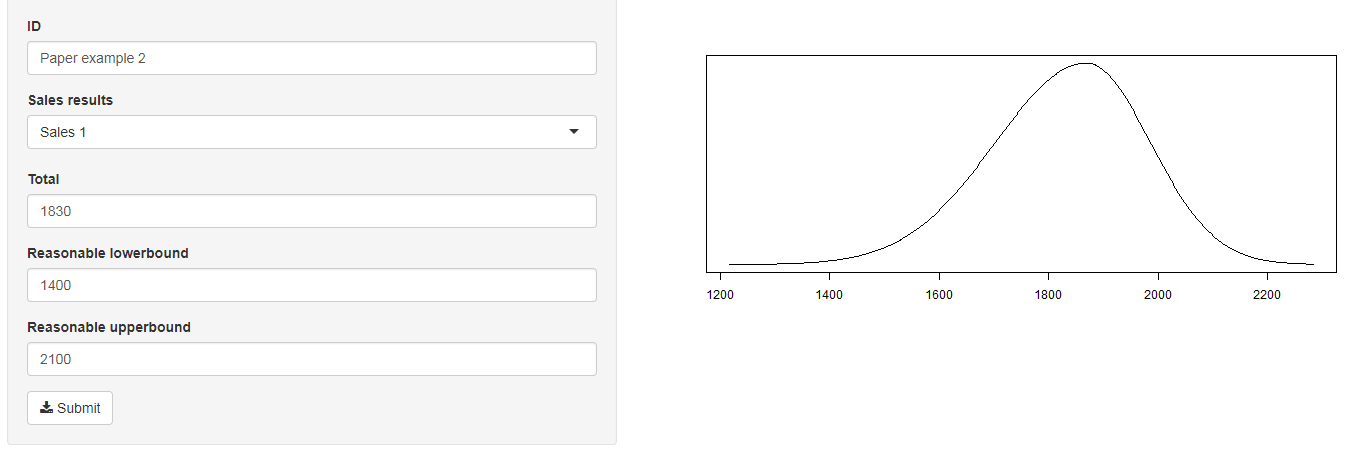
\includegraphics[width=0.9\linewidth]{figures/chapter_2/Figure_3} 

}

\caption{Shiny application for steps 3 and 4. On the left the input fields require entering the estimate for $\mu_0$ and the reasonable lower and upper bound for the estimate. On the right the distribution that is fitted based on the input can be found.}\label{fig:ch02fig3}
\end{figure}

\hypertarget{step-4}{%
\subsection{Step 4}\label{step-4}}

Based on the input provided in step 3 we will obtain estimates for the scale parameter \(\sigma^2_0\) and the shape parameter \(\gamma_0\). The 120 values, \(\mu_0\) repeated 100 times and the values for the reasonable lower and upper bounds both repeated 10 times, are provided to the snormFit function by means of which a SN distribution is fitted. The estimates for \(\sigma^2_0\) and \(\gamma_0\) are obtained and \(\mu_0\) is constrained to the input value. Visual feedback is provided to the expert of the resulting SN distribution, which can be seen in Figure \ref{fig:ch02fig3}. The expert can accept the representation of their beliefs or adjust input until the representation matches their beliefs.

\hypertarget{step-5}{%
\subsection{Step 5}\label{step-5}}

Use the elicited distribution that represents the expert's beliefs.

\hypertarget{elicitation-studies}{%
\section{Elicitation Studies}\label{elicitation-studies}}

In this section we describe the three studies we conducted. During the user feasibility study R version 3.1.2 was used and R version 3.2.3 was used during the elicitations done with the staffing company and the large financial institution. We conducted the elicitations in a semi-structured face-toface setting so that the researcher could provide interpretations accompanying the visual feedback. An advantage of a face-to-face setting is that it allows clarification of procedural and elicitation related questions thereby improving the validity of the responses (O'Hagan et al., \protect\hyperlink{ref-ohagan_uncertain_2006}{2006}).

(Cooke \& Goossens, \protect\hyperlink{ref-cooke_procedures_1999}{1999}) describe that a panel of four experts can be sufficient for an elicitation, but they recommend a panel of about eight experts as a rule of thumb. In the user feasibility study nine respondents participated. In the staffing company only four experts were available in the entire company, therefore the sample was limited to a size of four. Regarding the study at the large financial institution four experts participated in the end.

\hypertarget{user-feasibility-study}{%
\subsection{User Feasibility Study}\label{user-feasibility-study}}

\hypertarget{design}{%
\subsubsection{Design}\label{design}}

With the user feasibility study we evaluated the usability of the first two steps of the Five-Step Method. Procedural and visual preferences were investigated. Four variations of the shiny application were tested. The respondents (\(D=9\)), obtained through convenience sampling from a population of university trained adults, were randomly allocated to two out of the four possible variations of the software.

In the first procedural option, we used the procedure of the trial roulette where 20 digital ``chips'', starting with the expected minimal and maximum value, each representing five percent of a distribution, were to be placed in a grid following the procedure described by Zondervan-Zwijnenburg et al. (\protect\hyperlink{ref-zondervan-zwijnenburg_application_2017}{2017}\protect\hyperlink{ref-zondervan-zwijnenburg_application_2017}{b}). After placing 20 ``chips'' the respondents could submit their input and they were provided with visual feedback on the distribution that was fitted based on these 20 ``chips''. They could accept the representation or adjust their input. The second procedural option required the placement of a minimum of seven ``chips'', starting with the expected minimal and maximum value. In this procedural variation the distribution that was fitted based on the input was constantly shown. The distribution changed with each placed ``chip'' and thus instant feedback was provided on the representation of the input. Respondents could, after placing a minimum of seven ``chips'', at each point accept the representation of their beliefs or add or adjust input. Next to these two options, we also varied the size of the digital grid in which the ``chips''" were placed: large and small.

The respondents evaluated the two variations they were appointed to with a questionnaire asking if the fitted
distribution was a good reflection of their beliefs and what visual and procedural preferences were. Additional questions were based on the taxonomy of Bloom, Engelhart, Furst, Hill, \& Krathwohl (\protect\hyperlink{ref-bloom_taxonomy_1956}{1956}) to identify weak points of the software and procedures. These questions investigated; the comprehension of the instructions, the ability to apply the tool, the understanding of the representation of the ``chips''", the relation between input and fitted distribution, and the relation between belief and fitted distribution. The full questionnaire can be found in
the data archive which is available on the OSF webpage at \url{https://osf.io/wvujz}.

\hypertarget{results}{%
\subsubsection{Results}\label{results}}

All respondents indicated that their beliefs where accurately represented. Five of the seven respondents allocated to both procedural variants preferred the second variation. Four of the six respondents allocated to both visual variants preferred the large grid, one abstained from answering. Three out of the nine respondents indicated for at least one of the variations that they did not understand the meaning of the ``chips''. In
the first procedural option the ``chips'' each represented 5\% of the data whilst in the second procedural option the meaning depended on the amount of chips that were placed. They allocated mass for the distribution that was fitted. The meaning of the chips was not completely understood by one person who used the first procedure and by two persons who used the second procedure. All three of them used a small grid variation. The three respondents all indicated that they knew what the distribution representing their opinion meant in the end and agreed that this accurately described their view. Based on the results we decided to continue working with the second procedural variation, requiring the minimal placement of seven ``chips without further restriction on the number of''chips", and a large grid.

\hypertarget{elicitation-staffing-company}{%
\subsection{Elicitation Staffing Company}\label{elicitation-staffing-company}}

\hypertarget{design-1}{%
\subsubsection{Design}\label{design-1}}

The goal of the second study was to test the internal validity of elicitations obtained with the first two steps of the Five-Step Method. We found a staffing company willing to participate with experts (\(D=4\)) providing predictions about five sales results concerning the first quarter of 2016: contract hours, hourly cost buying and selling, turnover and hourly sales margin. A staffing company is a link between companies that want to hire staff and staff looking to work at companies. They buy work from individuals and thereafter place them to work at other companies. The amount of hours they place an individual at another company in the quarter are the contract hours. The hourly cost buying is what it will cost them per hour to buy the work from the individuals and the hourly cost selling is the price which they charge the companies where they stall the individuals. The turnover is equal to the contract hours multiplied by the hourly cost selling and the hourly sales margin is equal to the hourly cost selling minus the hourly cost buying.

The experts were asked to predict the distribution of the data. In some sectors staffing companies staff a lot of individuals at low margins and thus generate a large turnover. In different sectors they staff few individuals at high margins thereby obtaining the same profit at lower turnover rates. These are all relevant considerations and the experts should know which is the case for their company. The company provided us with actual budgets they made which were indications of carefully constructed predictions. By comparing the predictions of the experts to the budget we could gain an indication of the internal validity of predictions made with the first two steps of the Five-Step Method. If the elicitation results match the budget this indicates that the procedure is able to represent the underlying construct of carefully constructed predictions.

\hypertarget{results-1}{%
\subsubsection{Results}\label{results-1}}

The results can be found in Figure \ref{fig:ch02fig4} in which we plotted the predictions of the four experts against the actual budgets for the first quarter. To conceal the true values, which is businesssensitive information, a linear transformation has been done on all variables. It can be seen, especially for the hourly sales margins and the turnover, that experts provided very similar predictions to the budgets, for more detailed information see Table \ref{tab:ch02tab1}. The resemblance of the predictions to the budget indicates internal validity for the use of the steps 1 and 2 of the Five-Step Method as the elicited predictions closely match carefully constructed expectations. Based on these results we decided not to further adjust the elicitation procedure.

\begin{figure}

{\centering 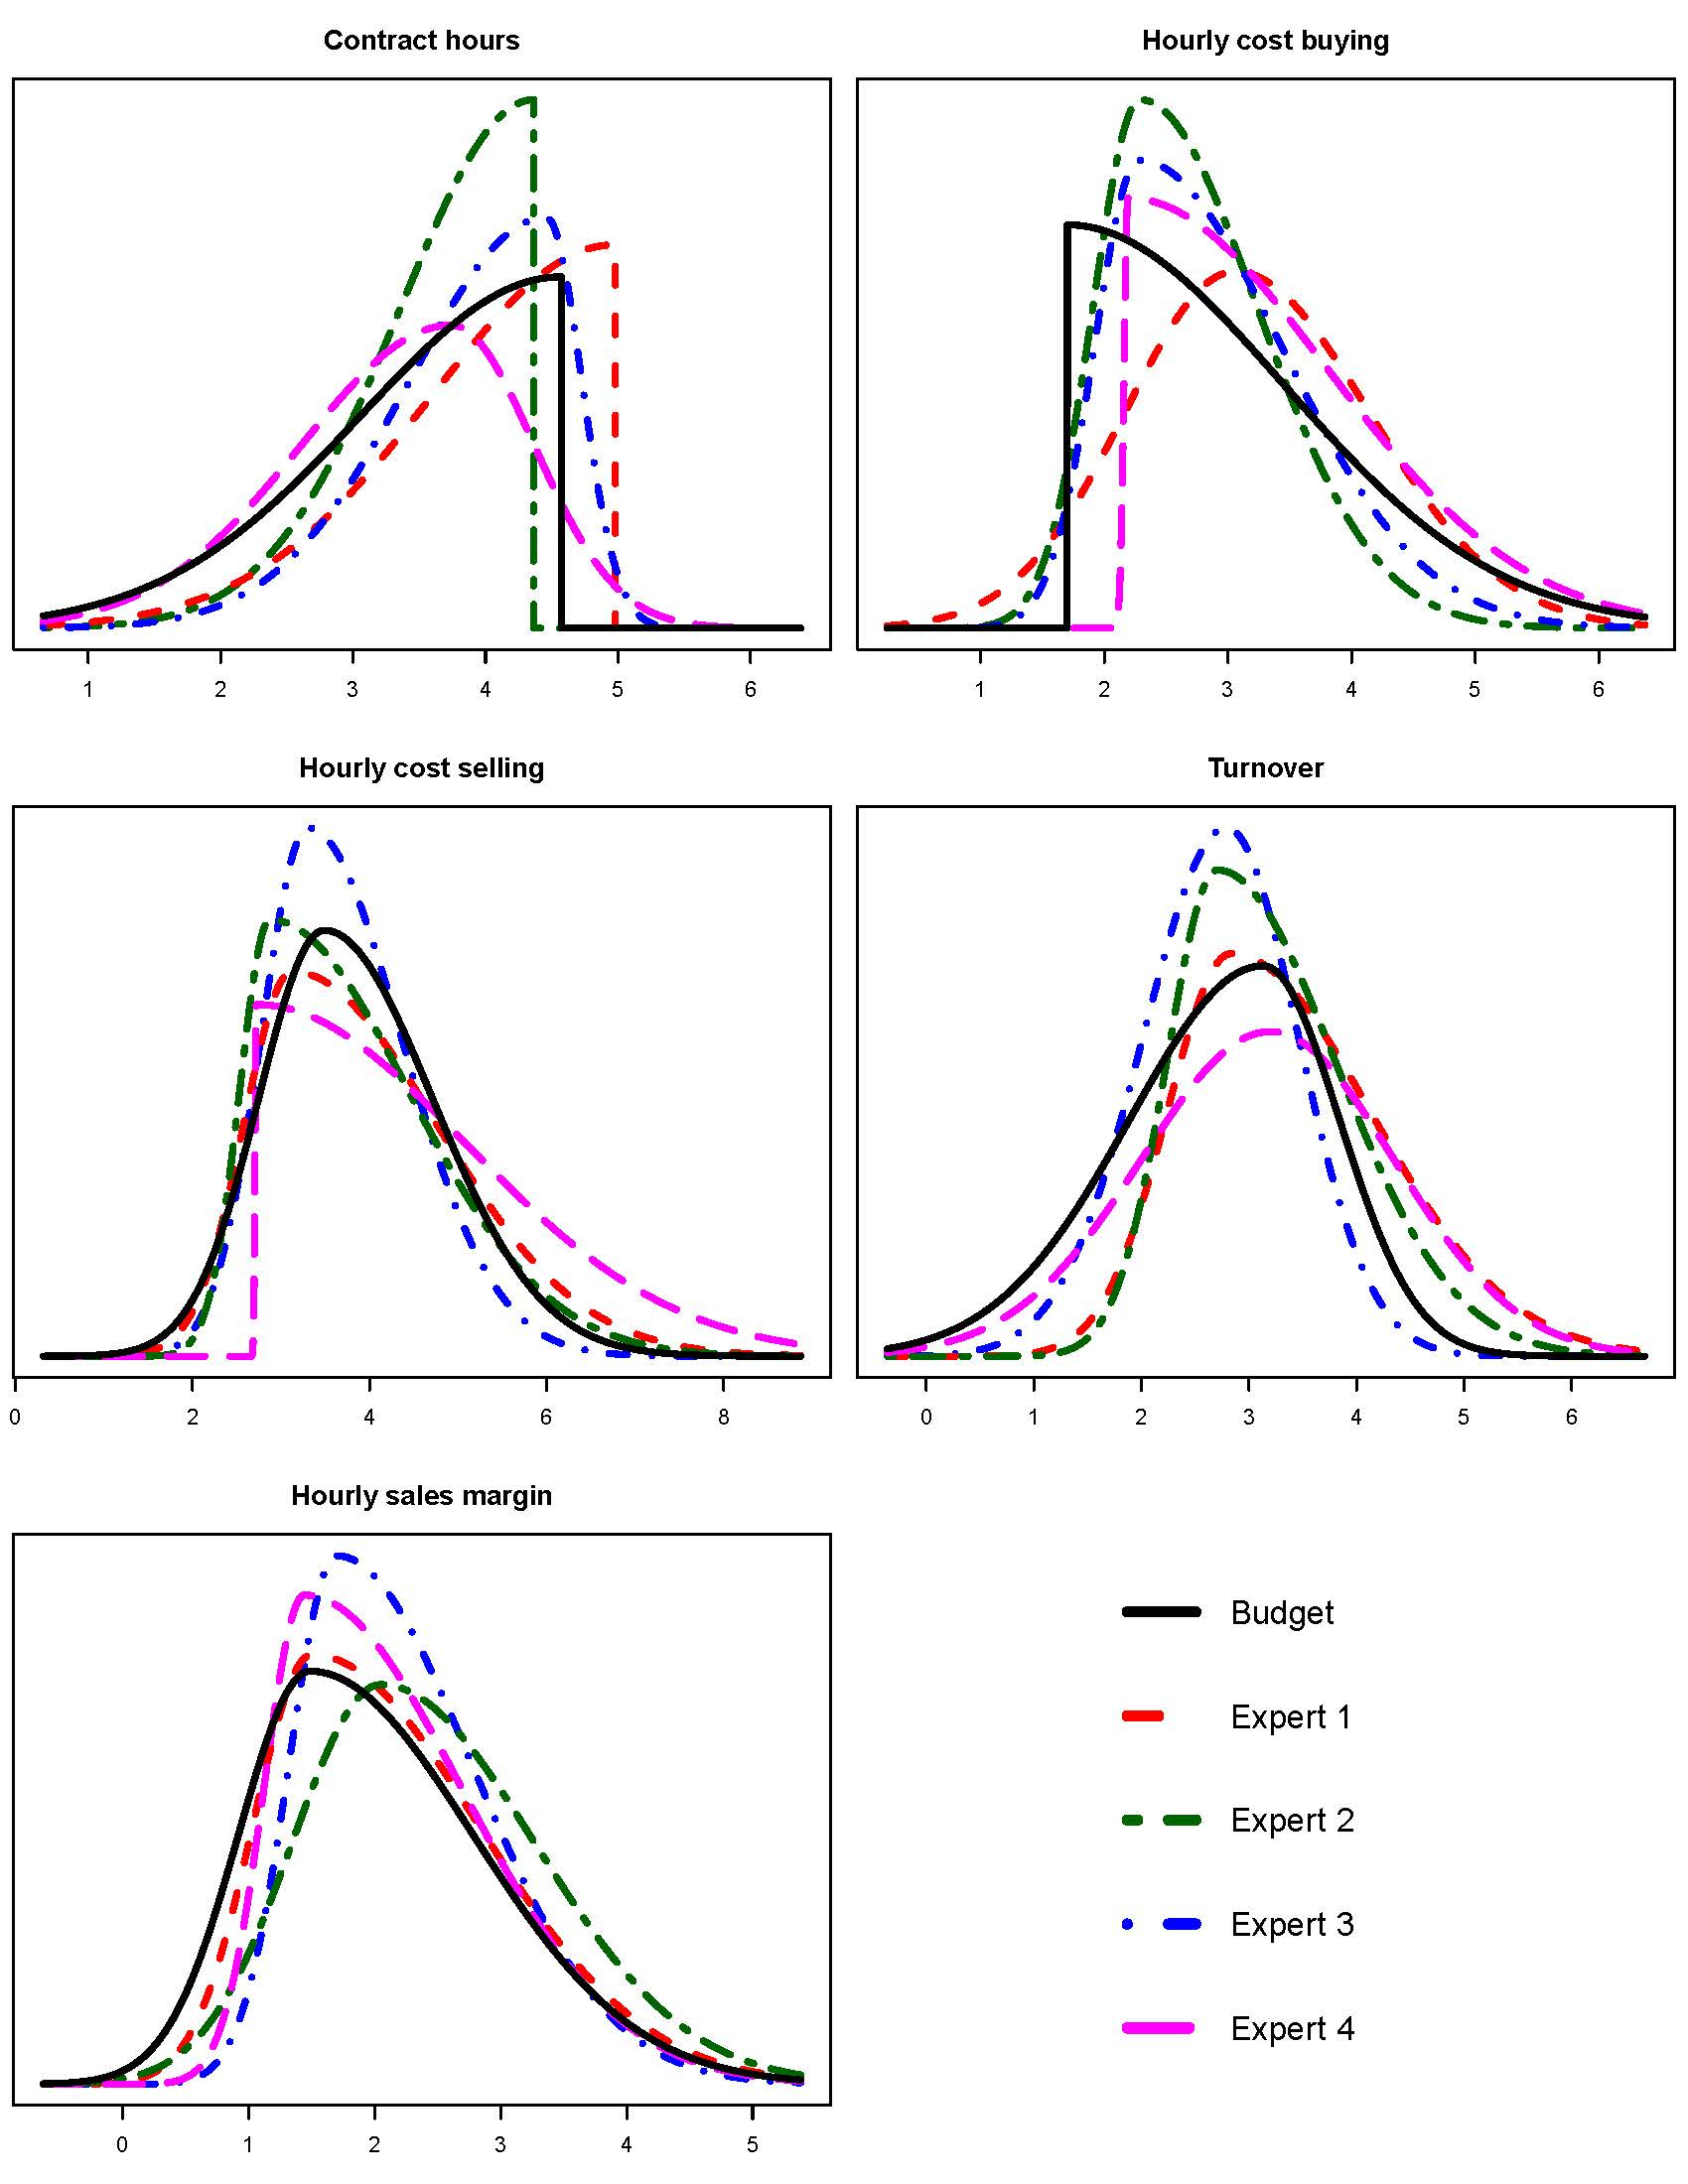
\includegraphics[width=0.75\linewidth]{figures/chapter_2/Figure_4} 

}

\caption{Results for elicitation with the staffing company. Experts' predictions plotted with actual budget for contract hours, hourly cost buying and selling, turnover and hourly sales margin concerning the first quarter of 2016.}\label{fig:ch02fig4}
\end{figure}

\newpage

\begin{longtable}[]{@{}llccc@{}}
\caption{\label{tab:ch02tab1} Results for elicitation with the staffing company. Experts' predictions with actual budget for contract hours, hourly cost buying and selling, turnover and hourly sales margin concerning the first quarter of 2016.}\tabularnewline
\toprule
\begin{minipage}[b]{0.30\columnwidth}\raggedright
\strut
\end{minipage} & \begin{minipage}[b]{0.13\columnwidth}\raggedright
\strut
\end{minipage} & \begin{minipage}[b]{0.10\columnwidth}\centering
\(\mu\)\strut
\end{minipage} & \begin{minipage}[b]{0.13\columnwidth}\centering
\(\sigma\)\strut
\end{minipage} & \begin{minipage}[b]{0.18\columnwidth}\centering
\(\gamma\)\strut
\end{minipage}\tabularnewline
\midrule
\endfirsthead
\toprule
\begin{minipage}[b]{0.30\columnwidth}\raggedright
\strut
\end{minipage} & \begin{minipage}[b]{0.13\columnwidth}\raggedright
\strut
\end{minipage} & \begin{minipage}[b]{0.10\columnwidth}\centering
\(\mu\)\strut
\end{minipage} & \begin{minipage}[b]{0.13\columnwidth}\centering
\(\sigma\)\strut
\end{minipage} & \begin{minipage}[b]{0.18\columnwidth}\centering
\(\gamma\)\strut
\end{minipage}\tabularnewline
\midrule
\endhead
\begin{minipage}[t]{0.30\columnwidth}\raggedright
\textbf{Contract}
\textbf{Hours}\strut
\end{minipage} & \begin{minipage}[t]{0.13\columnwidth}\raggedright
Expert 1\strut
\end{minipage} & \begin{minipage}[t]{0.10\columnwidth}\centering
3.88\strut
\end{minipage} & \begin{minipage}[t]{0.13\columnwidth}\centering
0.83\strut
\end{minipage} & \begin{minipage}[t]{0.18\columnwidth}\centering
4.01*10-6\strut
\end{minipage}\tabularnewline
\begin{minipage}[t]{0.30\columnwidth}\raggedright
\strut
\end{minipage} & \begin{minipage}[t]{0.13\columnwidth}\raggedright
Expert 2\strut
\end{minipage} & \begin{minipage}[t]{0.10\columnwidth}\centering
3.56\strut
\end{minipage} & \begin{minipage}[t]{0.13\columnwidth}\centering
0.61\strut
\end{minipage} & \begin{minipage}[t]{0.18\columnwidth}\centering
4.48*10-8\strut
\end{minipage}\tabularnewline
\begin{minipage}[t]{0.30\columnwidth}\raggedright
\strut
\end{minipage} & \begin{minipage}[t]{0.13\columnwidth}\raggedright
Expert 3\strut
\end{minipage} & \begin{minipage}[t]{0.10\columnwidth}\centering
3.85\strut
\end{minipage} & \begin{minipage}[t]{0.13\columnwidth}\centering
0.70\strut
\end{minipage} & \begin{minipage}[t]{0.18\columnwidth}\centering
0.51\strut
\end{minipage}\tabularnewline
\begin{minipage}[t]{0.30\columnwidth}\raggedright
\strut
\end{minipage} & \begin{minipage}[t]{0.13\columnwidth}\raggedright
Expert 4\strut
\end{minipage} & \begin{minipage}[t]{0.10\columnwidth}\centering
3.34\strut
\end{minipage} & \begin{minipage}[t]{0.13\columnwidth}\centering
0.89\strut
\end{minipage} & \begin{minipage}[t]{0.18\columnwidth}\centering
0.74\strut
\end{minipage}\tabularnewline
\begin{minipage}[t]{0.30\columnwidth}\raggedright
\strut
\end{minipage} & \begin{minipage}[t]{0.13\columnwidth}\raggedright
Budget\strut
\end{minipage} & \begin{minipage}[t]{0.10\columnwidth}\centering
3.37\strut
\end{minipage} & \begin{minipage}[t]{0.13\columnwidth}\centering
0.91\strut
\end{minipage} & \begin{minipage}[t]{0.18\columnwidth}\centering
5.52*10-4\strut
\end{minipage}\tabularnewline
\begin{minipage}[t]{0.30\columnwidth}\raggedright
\strut
\end{minipage} & \begin{minipage}[t]{0.13\columnwidth}\raggedright
\strut
\end{minipage} & \begin{minipage}[t]{0.10\columnwidth}\centering
\strut
\end{minipage} & \begin{minipage}[t]{0.13\columnwidth}\centering
\strut
\end{minipage} & \begin{minipage}[t]{0.18\columnwidth}\centering
\strut
\end{minipage}\tabularnewline
\begin{minipage}[t]{0.30\columnwidth}\raggedright
\textbf{Hourly Cost}
\textbf{Buying}\strut
\end{minipage} & \begin{minipage}[t]{0.13\columnwidth}\raggedright
Expert 1\strut
\end{minipage} & \begin{minipage}[t]{0.10\columnwidth}\centering
3.21\strut
\end{minipage} & \begin{minipage}[t]{0.13\columnwidth}\centering
0.99\strut
\end{minipage} & \begin{minipage}[t]{0.18\columnwidth}\centering
1.10\strut
\end{minipage}\tabularnewline
\begin{minipage}[t]{0.30\columnwidth}\raggedright
\strut
\end{minipage} & \begin{minipage}[t]{0.13\columnwidth}\raggedright
Expert 2\strut
\end{minipage} & \begin{minipage}[t]{0.10\columnwidth}\centering
2.74\strut
\end{minipage} & \begin{minipage}[t]{0.13\columnwidth}\centering
0.69\strut
\end{minipage} & \begin{minipage}[t]{0.18\columnwidth}\centering
1.57\strut
\end{minipage}\tabularnewline
\begin{minipage}[t]{0.30\columnwidth}\raggedright
\strut
\end{minipage} & \begin{minipage}[t]{0.13\columnwidth}\raggedright
Expert 3\strut
\end{minipage} & \begin{minipage}[t]{0.10\columnwidth}\centering
2.91\strut
\end{minipage} & \begin{minipage}[t]{0.13\columnwidth}\centering
0.80\strut
\end{minipage} & \begin{minipage}[t]{0.18\columnwidth}\centering
1.78\strut
\end{minipage}\tabularnewline
\begin{minipage}[t]{0.30\columnwidth}\raggedright
\strut
\end{minipage} & \begin{minipage}[t]{0.13\columnwidth}\raggedright
Expert 4\strut
\end{minipage} & \begin{minipage}[t]{0.10\columnwidth}\centering
3.45\strut
\end{minipage} & \begin{minipage}[t]{0.13\columnwidth}\centering
0.97\strut
\end{minipage} & \begin{minipage}[t]{0.18\columnwidth}\centering
7.20\strut
\end{minipage}\tabularnewline
\begin{minipage}[t]{0.30\columnwidth}\raggedright
\strut
\end{minipage} & \begin{minipage}[t]{0.13\columnwidth}\raggedright
Budget\strut
\end{minipage} & \begin{minipage}[t]{0.10\columnwidth}\centering
3.09\strut
\end{minipage} & \begin{minipage}[t]{0.13\columnwidth}\centering
1.05\strut
\end{minipage} & \begin{minipage}[t]{0.18\columnwidth}\centering
566.00\strut
\end{minipage}\tabularnewline
\begin{minipage}[t]{0.30\columnwidth}\raggedright
\strut
\end{minipage} & \begin{minipage}[t]{0.13\columnwidth}\raggedright
\strut
\end{minipage} & \begin{minipage}[t]{0.10\columnwidth}\centering
\strut
\end{minipage} & \begin{minipage}[t]{0.13\columnwidth}\centering
\strut
\end{minipage} & \begin{minipage}[t]{0.18\columnwidth}\centering
\strut
\end{minipage}\tabularnewline
\begin{minipage}[t]{0.30\columnwidth}\raggedright
\textbf{Hourly Cost}
\textbf{Selling}\strut
\end{minipage} & \begin{minipage}[t]{0.13\columnwidth}\raggedright
Expert 1\strut
\end{minipage} & \begin{minipage}[t]{0.10\columnwidth}\centering
3.99\strut
\end{minipage} & \begin{minipage}[t]{0.13\columnwidth}\centering
1.14\strut
\end{minipage} & \begin{minipage}[t]{0.18\columnwidth}\centering
1.73\strut
\end{minipage}\tabularnewline
\begin{minipage}[t]{0.30\columnwidth}\raggedright
\strut
\end{minipage} & \begin{minipage}[t]{0.13\columnwidth}\raggedright
Expert 2\strut
\end{minipage} & \begin{minipage}[t]{0.10\columnwidth}\centering
3.86\strut
\end{minipage} & \begin{minipage}[t]{0.13\columnwidth}\centering
1.04\strut
\end{minipage} & \begin{minipage}[t]{0.18\columnwidth}\centering
2.14\strut
\end{minipage}\tabularnewline
\begin{minipage}[t]{0.30\columnwidth}\raggedright
\strut
\end{minipage} & \begin{minipage}[t]{0.13\columnwidth}\raggedright
Expert 3\strut
\end{minipage} & \begin{minipage}[t]{0.10\columnwidth}\centering
3.72\strut
\end{minipage} & \begin{minipage}[t]{0.13\columnwidth}\centering
0.81\strut
\end{minipage} & \begin{minipage}[t]{0.18\columnwidth}\centering
1.41\strut
\end{minipage}\tabularnewline
\begin{minipage}[t]{0.30\columnwidth}\raggedright
\strut
\end{minipage} & \begin{minipage}[t]{0.13\columnwidth}\raggedright
Expert 4\strut
\end{minipage} & \begin{minipage}[t]{0.10\columnwidth}\centering
4.59\strut
\end{minipage} & \begin{minipage}[t]{0.13\columnwidth}\centering
1.43\strut
\end{minipage} & \begin{minipage}[t]{0.18\columnwidth}\centering
12.80\strut
\end{minipage}\tabularnewline
\begin{minipage}[t]{0.30\columnwidth}\raggedright
\strut
\end{minipage} & \begin{minipage}[t]{0.13\columnwidth}\raggedright
Budget\strut
\end{minipage} & \begin{minipage}[t]{0.10\columnwidth}\centering
3.87\strut
\end{minipage} & \begin{minipage}[t]{0.13\columnwidth}\centering
0.99\strut
\end{minipage} & \begin{minipage}[t]{0.18\columnwidth}\centering
1.29\strut
\end{minipage}\tabularnewline
\begin{minipage}[t]{0.30\columnwidth}\raggedright
\strut
\end{minipage} & \begin{minipage}[t]{0.13\columnwidth}\raggedright
\strut
\end{minipage} & \begin{minipage}[t]{0.10\columnwidth}\centering
\strut
\end{minipage} & \begin{minipage}[t]{0.13\columnwidth}\centering
\strut
\end{minipage} & \begin{minipage}[t]{0.18\columnwidth}\centering
\strut
\end{minipage}\tabularnewline
\begin{minipage}[t]{0.30\columnwidth}\raggedright
\textbf{Turnover}\strut
\end{minipage} & \begin{minipage}[t]{0.13\columnwidth}\raggedright
Expert 1\strut
\end{minipage} & \begin{minipage}[t]{0.10\columnwidth}\centering
3.39\strut
\end{minipage} & \begin{minipage}[t]{0.13\columnwidth}\centering
0.98\strut
\end{minipage} & \begin{minipage}[t]{0.18\columnwidth}\centering
1.48\strut
\end{minipage}\tabularnewline
\begin{minipage}[t]{0.30\columnwidth}\raggedright
\strut
\end{minipage} & \begin{minipage}[t]{0.13\columnwidth}\raggedright
Expert 2\strut
\end{minipage} & \begin{minipage}[t]{0.10\columnwidth}\centering
3.21\strut
\end{minipage} & \begin{minipage}[t]{0.13\columnwidth}\centering
0.81\strut
\end{minipage} & \begin{minipage}[t]{0.18\columnwidth}\centering
1.53\strut
\end{minipage}\tabularnewline
\begin{minipage}[t]{0.30\columnwidth}\raggedright
\strut
\end{minipage} & \begin{minipage}[t]{0.13\columnwidth}\raggedright
Expert 3\strut
\end{minipage} & \begin{minipage}[t]{0.10\columnwidth}\centering
2.71\strut
\end{minipage} & \begin{minipage}[t]{0.13\columnwidth}\centering
0.72\strut
\end{minipage} & \begin{minipage}[t]{0.18\columnwidth}\centering
0.93\strut
\end{minipage}\tabularnewline
\begin{minipage}[t]{0.30\columnwidth}\raggedright
\strut
\end{minipage} & \begin{minipage}[t]{0.13\columnwidth}\raggedright
Expert 4\strut
\end{minipage} & \begin{minipage}[t]{0.10\columnwidth}\centering
3.16\strut
\end{minipage} & \begin{minipage}[t]{0.13\columnwidth}\centering
1.17\strut
\end{minipage} & \begin{minipage}[t]{0.18\columnwidth}\centering
0.98\strut
\end{minipage}\tabularnewline
\begin{minipage}[t]{0.30\columnwidth}\raggedright
\strut
\end{minipage} & \begin{minipage}[t]{0.13\columnwidth}\raggedright
Budget\strut
\end{minipage} & \begin{minipage}[t]{0.10\columnwidth}\centering
2.71\strut
\end{minipage} & \begin{minipage}[t]{0.13\columnwidth}\centering
0.99\strut
\end{minipage} & \begin{minipage}[t]{0.18\columnwidth}\centering
0.76\strut
\end{minipage}\tabularnewline
\begin{minipage}[t]{0.30\columnwidth}\raggedright
\strut
\end{minipage} & \begin{minipage}[t]{0.13\columnwidth}\raggedright
\strut
\end{minipage} & \begin{minipage}[t]{0.10\columnwidth}\centering
\strut
\end{minipage} & \begin{minipage}[t]{0.13\columnwidth}\centering
\strut
\end{minipage} & \begin{minipage}[t]{0.18\columnwidth}\centering
\strut
\end{minipage}\tabularnewline
\begin{minipage}[t]{0.30\columnwidth}\raggedright
\textbf{Hourly}
\textbf{Sales}
\textbf{Margin}\strut
\end{minipage} & \begin{minipage}[t]{0.13\columnwidth}\raggedright
Expert 1\strut
\end{minipage} & \begin{minipage}[t]{0.10\columnwidth}\centering
2.18\strut
\end{minipage} & \begin{minipage}[t]{0.13\columnwidth}\centering
0.94\strut
\end{minipage} & \begin{minipage}[t]{0.18\columnwidth}\centering
1.68\strut
\end{minipage}\tabularnewline
\begin{minipage}[t]{0.30\columnwidth}\raggedright
\strut
\end{minipage} & \begin{minipage}[t]{0.13\columnwidth}\raggedright
Expert 2\strut
\end{minipage} & \begin{minipage}[t]{0.10\columnwidth}\centering
2.46\strut
\end{minipage} & \begin{minipage}[t]{0.13\columnwidth}\centering
0.97\strut
\end{minipage} & \begin{minipage}[t]{0.18\columnwidth}\centering
1.31\strut
\end{minipage}\tabularnewline
\begin{minipage}[t]{0.30\columnwidth}\raggedright
\strut
\end{minipage} & \begin{minipage}[t]{0.13\columnwidth}\raggedright
Expert 3\strut
\end{minipage} & \begin{minipage}[t]{0.10\columnwidth}\centering
2.25\strut
\end{minipage} & \begin{minipage}[t]{0.13\columnwidth}\centering
0.76\strut
\end{minipage} & \begin{minipage}[t]{0.18\columnwidth}\centering
1.69\strut
\end{minipage}\tabularnewline
\begin{minipage}[t]{0.30\columnwidth}\raggedright
\strut
\end{minipage} & \begin{minipage}[t]{0.13\columnwidth}\raggedright
Expert 4\strut
\end{minipage} & \begin{minipage}[t]{0.10\columnwidth}\centering
2.18\strut
\end{minipage} & \begin{minipage}[t]{0.13\columnwidth}\centering
0.84\strut
\end{minipage} & \begin{minipage}[t]{0.18\columnwidth}\centering
1.97\strut
\end{minipage}\tabularnewline
\begin{minipage}[t]{0.30\columnwidth}\raggedright
\strut
\end{minipage} & \begin{minipage}[t]{0.13\columnwidth}\raggedright
Budget\strut
\end{minipage} & \begin{minipage}[t]{0.10\columnwidth}\centering
2.06\strut
\end{minipage} & \begin{minipage}[t]{0.13\columnwidth}\centering
0.96\strut
\end{minipage} & \begin{minipage}[t]{0.18\columnwidth}\centering
1.51\strut
\end{minipage}\tabularnewline
\bottomrule
\end{longtable}

\newpage

\hypertarget{elicitation-large-financial-institution}{%
\subsection{Elicitation Large Financial Institution}\label{elicitation-large-financial-institution}}

In the third elicitation study the experts (\(D=4\)) were regional directors working at a large financial institution. They are considered experts in knowledge concerning market opportunities, market dynamics and estimating the capabilities of the professionals to seize opportunities. Based on these skills we expected that they could predict the average turnover per professional in the entire country in the first quarter of 2016. In this study the experts did not predict the distribution of the data \(\textbf{y}\), but construct a prior for the mean denoted by \(\pi_d(\theta)\). As \(\pi_d(\theta) \sim SN(\mu_0, \sigma^2_0, \gamma_0)\) the elicitation results in the representation of each expert's beliefs expressed in the hyper parameters \(\mu_0\), \(\sigma^2_0\) and \(\gamma_0\). We compare the predictions of the experts against actual results, expressed as the posterior distribution of the average turnover per professional, denoted by \(\pi(\theta|y)\). \(\pi(\theta|y) \sim SN(\mu_1, \sigma^2_1, \gamma_1)\), \(\mu_1\) denotes the posterior mean, \(\sigma^2_1\) denotes the posterior variance and \(\gamma1\) the posterior skewness. The prior for \(\pi(\theta|y)\) is a \(N(0,100)\) prior which is uninformative given the scale of the data.

\hypertarget{design-2}{%
\subsubsection{Design}\label{design-2}}

The team that participated consisted of 11 experts, 10 regional directors and one director. All were eligible to be included in the study. To comply with conditions set by the Ethics Committee, we ensured that experts whom did not wish to participate could do so without it being known that they refused. Therefore we randomly selected seven out of the 11 experts and invited them to participate. Out of the seven selected experts that we approached, three indicated that they did not want to participate in the study and four indicated that they were willing to participate. All four experts that agreed to participate, did participate and completed the elicitation. The participating experts first performed a practice elicitation for their own sales team before moving on to their estimate for the whole country, enabling them to acquaint themselves with the elicitation applications. Offering this practice elicitation could improve the quality of the elicitations (Johnson et al., \protect\hyperlink{ref-johnson_methods_2010}{2010}). Only in the case that the director participated the practice run was be possible. The study receive ethical approval from our internal Ethics Committee of the Faculty of Social and Behavioural Sciences of Utrecht University. The letter of approval can be found in the data archive on the OSF website at \url{https://osf.io/wvujz}.

The Five-Step Method was used in this elicitation study and it consists of the following two parts: the first step is designed to support the expert in the use of reasoned and structured thoughts to obtain an estimate for the location parameter \(\mu_0\). In the second step the estimate for \(\mu_0\) is used and the expert is asked to provide a reasonable lower and upper bound for their estimate so the prior distribution for the mean turnover per professional can be constructed.

The ``chips'' placed in the first step were intended to represent individual professionals in the trial run and
clusters of similar professionals in the elicitation concerning the whole country. Visual feedback was provided on the elicited distribution, accompanied by a description of the value for \(\mu_0\) by the researcher. The expert could accept the representation of their beliefs or adjust input until the representation matched their beliefs. Results concerning country wide performance where discussed in terms of total turnover for all professionals within the team, therefore the estimate for \(\mu_0\) was transformed using the following function

\begin{equation} 
\theta^* = a\theta + b,
\label{eq:ch02eq2}
\end{equation}
where \(\theta\) represents the parameter of interest and \(\theta \sim N(\mu, \sigma^2)\) so that \(\theta^* \sim N[a\mu + b, (a\sigma)^2]\).

The use of the mean as location parameter offered additional options to accommodate differences in reasoning of experts, e.g., a sales expert might feel comfortable to provide estimates for the total turnover of a store, represented by \(\theta^*\) in Eq. \eqref{eq:ch02eq2}, but not be comfortable providing estimates for the mean turnover per product sold in the store, represented by \(\theta\) in Eq. \eqref{eq:ch02eq2}. By knowing the total amount of products that are sold in the store, entering the amount as value for a and 0 for b in Eq. \eqref{eq:ch02eq2}, the prior beliefs regarding the total turnover can be transformed to prior beliefs regarding mean turnover per product and compared to predictions by other experts. The transformation procedure ensures no expert is forced to adhere to a certain scale. To illustrate this flexibility let us imagine that a store sells nine different types of products and in total sells 104 products. In steps 1 and 2 we wish to elicit and verify the location parameter for the mean turnover. Two experts feel comfortable supplying estimates for turnover per product whilst two other experts only feel comfortable supplying estimates for turnover per product type. They can both adhere to the scale they feel comfortable with as we can use a linear transformation to get them onto the same scale for steps 3 and 4. In Table \ref{tab:ch02tab2} we supply a numerical example to show how location parameters, elicited on a different scale, can be transformed using Eq. \eqref{eq:ch02eq2} to be on the same scale for steps three and four of the elicitation.

In step 3 of the Five-Step Method, we asked the experts to provide a reasonable lower and upper bound for the total turnover of all professionals: Based on the input a distribution was fitted and visual feedback was provided. The researcher supported the visual feedback with a description explaining that more density on places of the axis indicate more perceived likeliness for that value. The expert could accept the representation of their beliefs or adjust the input for the reasonable lower and upper bound until the representation matched their beliefs. The elicited distribution was transformed back to represent the average turnover per professional using Eq. \eqref{eq:ch02eq2}.

\begin{longtable}[]{@{}lcccc@{}}
\caption{\label{tab:ch02tab2} Illustration of linear transformations using Eq. \eqref{eq:ch02eq2}. Experts 1 and 2 choose to specify turnover per product, resulting in a location parameter on the product scale. Experts 3 and 4 choose to specify turnover per product type, resulting in a location parameter on the product type scale. In steps 3 and 4 we can use either the location parameter on the total turnover scale or the mean turnover scale for experts to provide a reasonable lower and upper bound. All experts' elicited location parameters can be transformed to both scales.}\tabularnewline
\toprule
\begin{minipage}[b]{0.16\columnwidth}\raggedright
\strut
\end{minipage} & \begin{minipage}[b]{0.16\columnwidth}\centering
Steps 1 and 2
product scale
mean result
\((n=104)\)\strut
\end{minipage} & \begin{minipage}[b]{0.17\columnwidth}\centering
Steps 1 and 2
product type
scale mean
result \((n=9)\)\strut
\end{minipage} & \begin{minipage}[b]{0.17\columnwidth}\centering
Mean turnover
per product
used in steps
3 and 4\strut
\end{minipage} & \begin{minipage}[b]{0.17\columnwidth}\centering
Total turnover
used in steps
3 and 4\strut
\end{minipage}\tabularnewline
\midrule
\endfirsthead
\toprule
\begin{minipage}[b]{0.16\columnwidth}\raggedright
\strut
\end{minipage} & \begin{minipage}[b]{0.16\columnwidth}\centering
Steps 1 and 2
product scale
mean result
\((n=104)\)\strut
\end{minipage} & \begin{minipage}[b]{0.17\columnwidth}\centering
Steps 1 and 2
product type
scale mean
result \((n=9)\)\strut
\end{minipage} & \begin{minipage}[b]{0.17\columnwidth}\centering
Mean turnover
per product
used in steps
3 and 4\strut
\end{minipage} & \begin{minipage}[b]{0.17\columnwidth}\centering
Total turnover
used in steps
3 and 4\strut
\end{minipage}\tabularnewline
\midrule
\endhead
\begin{minipage}[t]{0.16\columnwidth}\raggedright
Expert 1\strut
\end{minipage} & \begin{minipage}[t]{0.16\columnwidth}\centering
1.8\strut
\end{minipage} & \begin{minipage}[t]{0.17\columnwidth}\centering
-\strut
\end{minipage} & \begin{minipage}[t]{0.17\columnwidth}\centering
1.80\strut
\end{minipage} & \begin{minipage}[t]{0.17\columnwidth}\centering
187.2\strut
\end{minipage}\tabularnewline
\begin{minipage}[t]{0.16\columnwidth}\raggedright
Expert 2\strut
\end{minipage} & \begin{minipage}[t]{0.16\columnwidth}\centering
2.1\strut
\end{minipage} & \begin{minipage}[t]{0.17\columnwidth}\centering
--\strut
\end{minipage} & \begin{minipage}[t]{0.17\columnwidth}\centering
2.10\strut
\end{minipage} & \begin{minipage}[t]{0.17\columnwidth}\centering
218.4\strut
\end{minipage}\tabularnewline
\begin{minipage}[t]{0.16\columnwidth}\raggedright
Expert 3\strut
\end{minipage} & \begin{minipage}[t]{0.16\columnwidth}\centering
-\strut
\end{minipage} & \begin{minipage}[t]{0.17\columnwidth}\centering
23\strut
\end{minipage} & \begin{minipage}[t]{0.17\columnwidth}\centering
1.99\strut
\end{minipage} & \begin{minipage}[t]{0.17\columnwidth}\centering
207\strut
\end{minipage}\tabularnewline
\begin{minipage}[t]{0.16\columnwidth}\raggedright
Expert 4\strut
\end{minipage} & \begin{minipage}[t]{0.16\columnwidth}\centering
--\strut
\end{minipage} & \begin{minipage}[t]{0.17\columnwidth}\centering
24.5\strut
\end{minipage} & \begin{minipage}[t]{0.17\columnwidth}\centering
2.12\strut
\end{minipage} & \begin{minipage}[t]{0.17\columnwidth}\centering
220.5\strut
\end{minipage}\tabularnewline
\bottomrule
\end{longtable}

\hypertarget{results-2}{%
\subsubsection{Results}\label{results-2}}

During the elicitation procedures we noticed that not all experts reasoned in the same way. One expert reasoned for his own region in the expected elements, such that each ``chip'' represented a professional, but concerning the elicitation for the whole country the ``chips'' represented regional performances not clusters of professionals that are alike. This deviation did not require an adjustment of procedure just a different value for a in Eq. \eqref{eq:ch02eq2} to obtain the estimate for total turnover used in step 3 of the Five-Step Method. Another expert directly reasoned in total turnover when considering country wide performance and directly provided the estimate used in step 3. A third expert started, especially during the test run concerning the expert's own team, naming the professionals aloud whilst placing the ``chips'',using the expected representations for the input. The procedure proved flexible enough so that each expert could use their own careful reasoning within the same framework and end up with comparable output.

All data were analyzed anonymously and were transformed to avoid revealing business-sensitive information. The elicited priors \(\pi_d(\theta)\) can be found in Figure \ref{fig:ch02fig5}, together with the posterior distribution \(\pi(\theta|y)\). The values for the hyper parameters for \(\pi_d(\theta)\) and \(\pi(\theta|y)\) can be found in Table \ref{tab:ch02tab3}. We can see, visually in Figure \ref{fig:ch02fig5} and numerically in Table \ref{tab:ch02tab3}, that experts one and two provide very similar predictions, however expert 2 is less uncertain about the prediction. In the same manner we can see that expert four made a prediction that closely resembles the actual realization.

\begin{figure}

{\centering 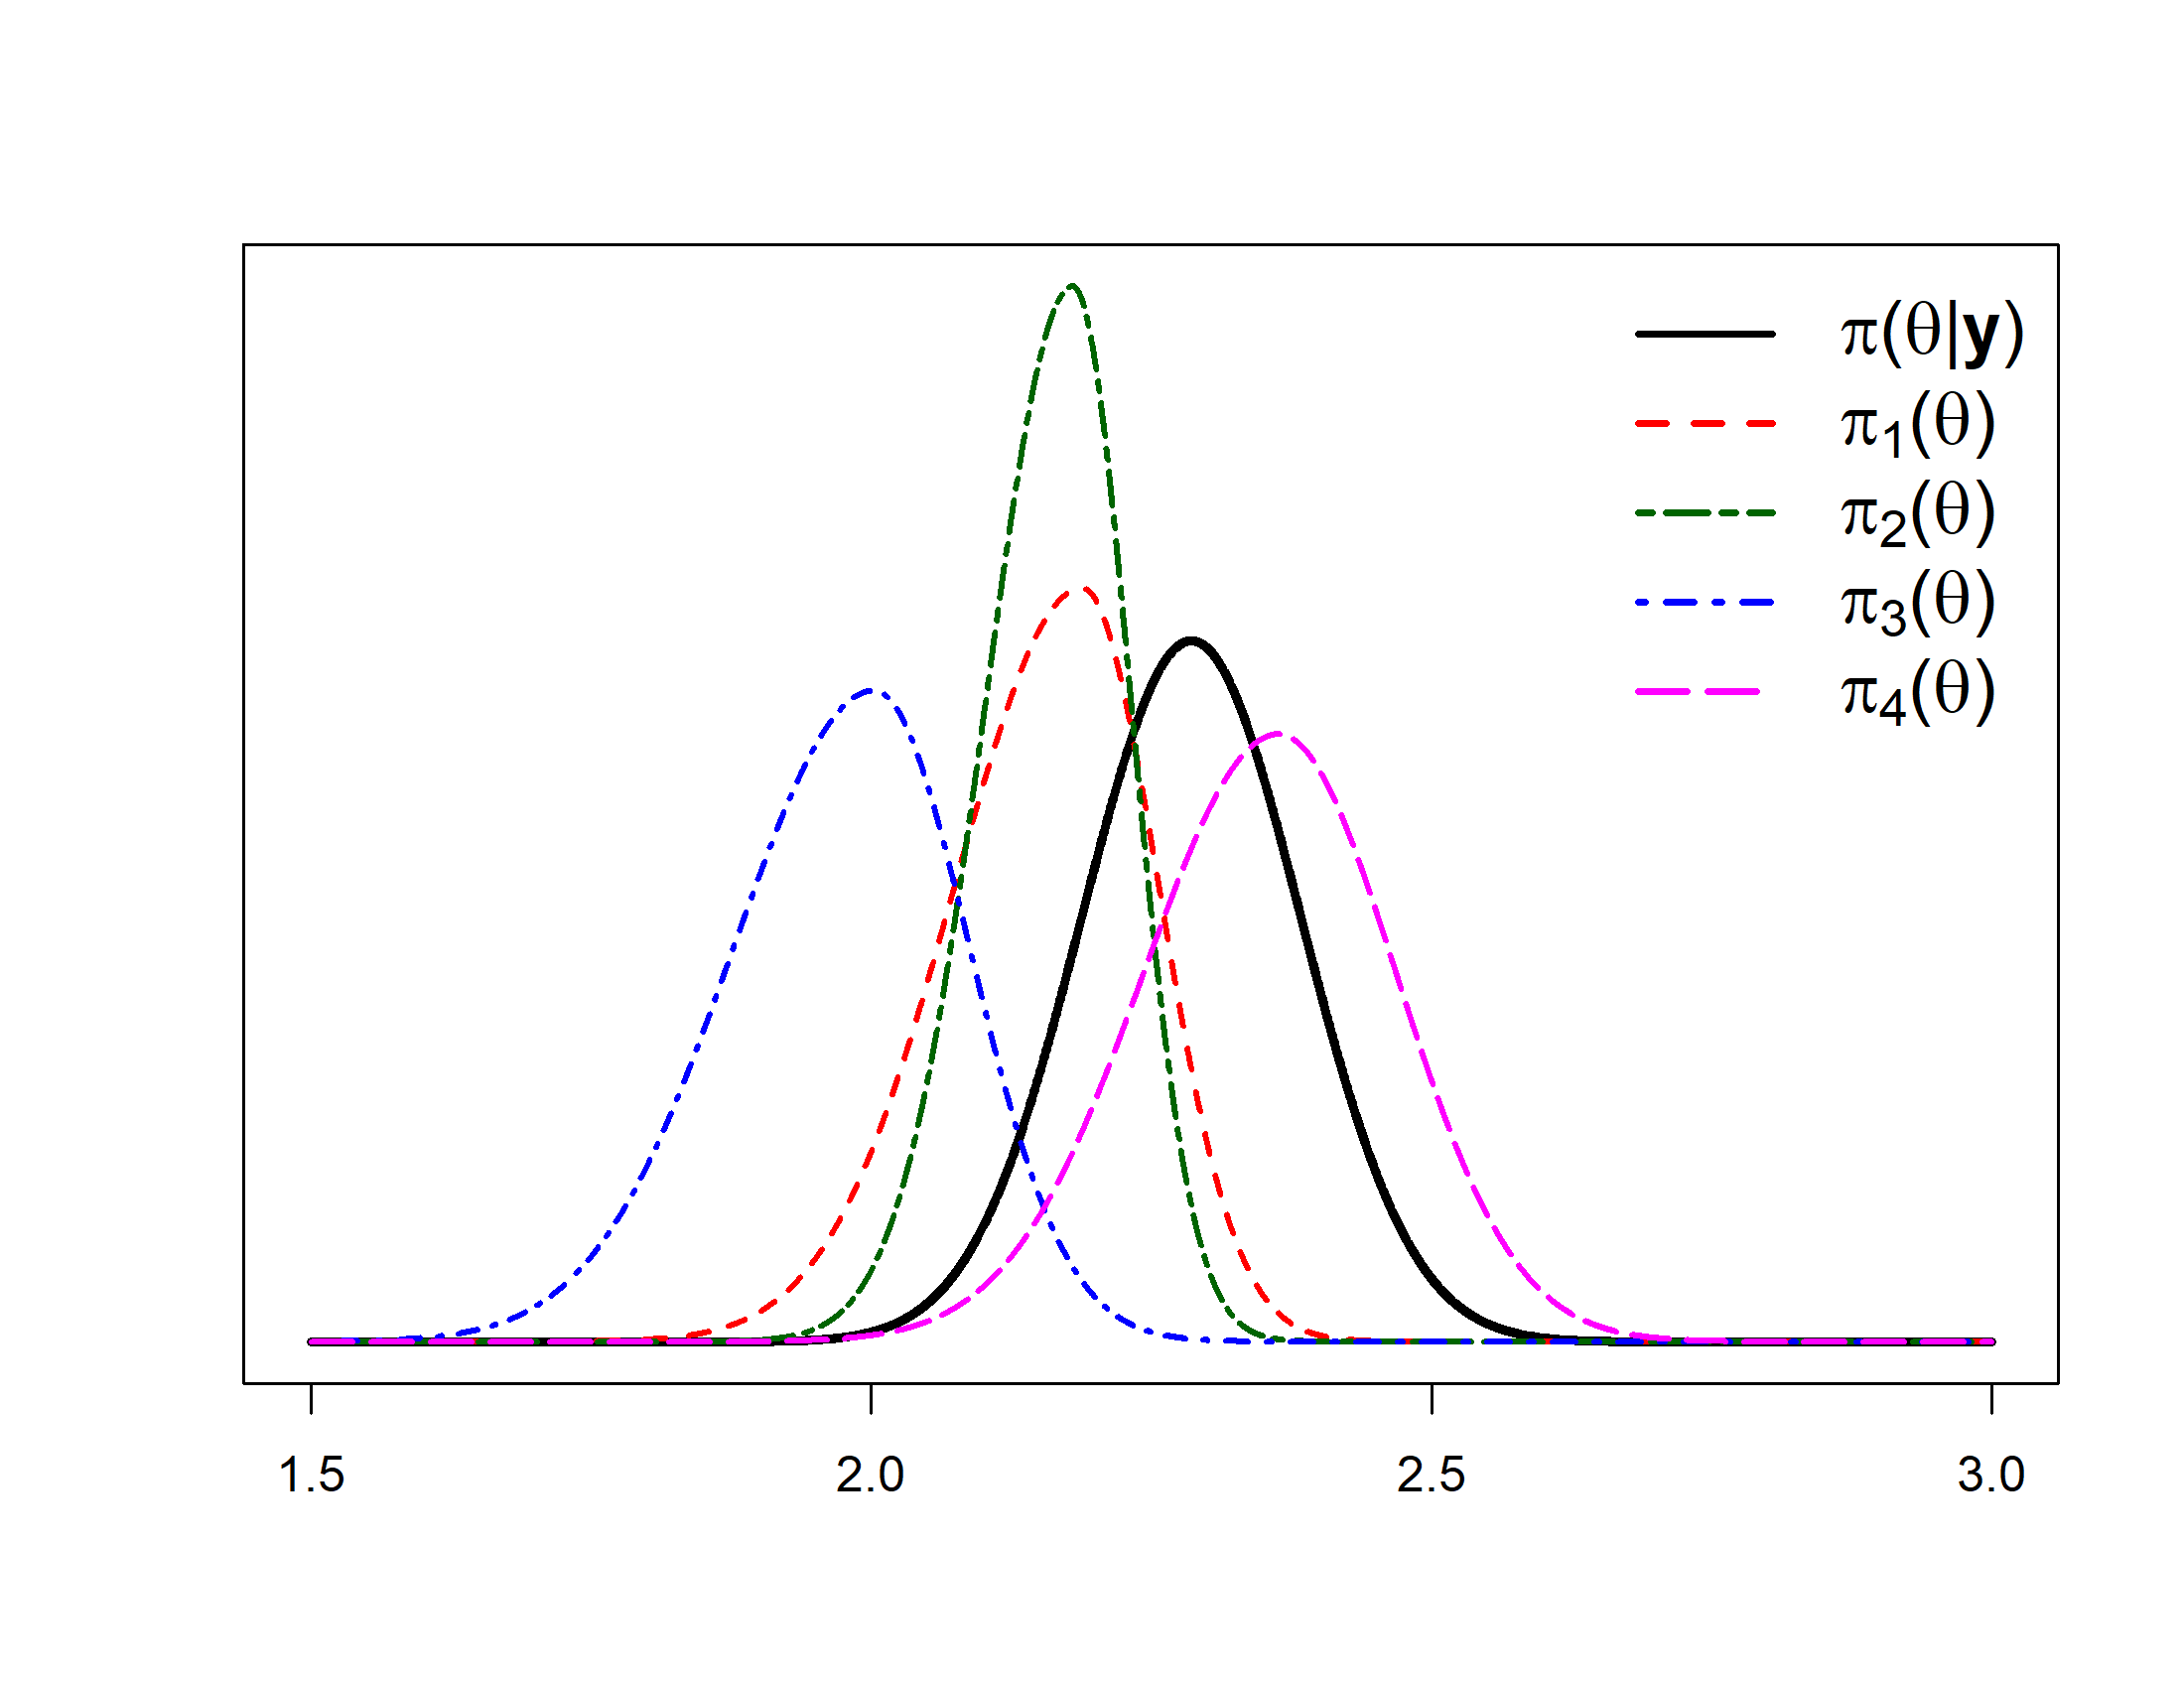
\includegraphics[width=0.9\linewidth]{figures/chapter_2/Figure_5a} 

}

\caption{Results Five-Step Method elicitation study with large financial institution. Elicited expert distributions $\pi_d(\theta)$ plotted with results $\pi(\theta|y)$.}\label{fig:ch02fig5}
\end{figure}

\begin{longtable}[]{@{}lcccccc@{}}
\caption{\label{tab:ch02tab3} The values of the hyper parameters of \(\pi(\theta|y)\) and \(\pi_d(\theta)\) for the study with the large financial institution.}\tabularnewline
\toprule
\begin{minipage}[b]{0.14\columnwidth}\raggedright
\strut
\end{minipage} & \begin{minipage}[b]{0.10\columnwidth}\centering
\(\mu_0\)\strut
\end{minipage} & \begin{minipage}[b]{0.12\columnwidth}\centering
\(\sigma_0\)\strut
\end{minipage} & \begin{minipage}[b]{0.12\columnwidth}\centering
\(\gamma_0\)\strut
\end{minipage} & \begin{minipage}[b]{0.09\columnwidth}\centering
\(\mu_1\)\strut
\end{minipage} & \begin{minipage}[b]{0.12\columnwidth}\centering
\(\sigma_1\)\strut
\end{minipage} & \begin{minipage}[b]{0.12\columnwidth}\centering
\(\gamma_1\)\strut
\end{minipage}\tabularnewline
\midrule
\endfirsthead
\toprule
\begin{minipage}[b]{0.14\columnwidth}\raggedright
\strut
\end{minipage} & \begin{minipage}[b]{0.10\columnwidth}\centering
\(\mu_0\)\strut
\end{minipage} & \begin{minipage}[b]{0.12\columnwidth}\centering
\(\sigma_0\)\strut
\end{minipage} & \begin{minipage}[b]{0.12\columnwidth}\centering
\(\gamma_0\)\strut
\end{minipage} & \begin{minipage}[b]{0.09\columnwidth}\centering
\(\mu_1\)\strut
\end{minipage} & \begin{minipage}[b]{0.12\columnwidth}\centering
\(\sigma_1\)\strut
\end{minipage} & \begin{minipage}[b]{0.12\columnwidth}\centering
\(\gamma_1\)\strut
\end{minipage}\tabularnewline
\midrule
\endhead
\begin{minipage}[t]{0.14\columnwidth}\raggedright
Preferred
distribution\strut
\end{minipage} & \begin{minipage}[t]{0.10\columnwidth}\centering
--\strut
\end{minipage} & \begin{minipage}[t]{0.12\columnwidth}\centering
--\strut
\end{minipage} & \begin{minipage}[t]{0.12\columnwidth}\centering
--\strut
\end{minipage} & \begin{minipage}[t]{0.09\columnwidth}\centering
2.29\strut
\end{minipage} & \begin{minipage}[t]{0.12\columnwidth}\centering
0.10\strut
\end{minipage} & \begin{minipage}[t]{0.12\columnwidth}\centering
0.99\strut
\end{minipage}\tabularnewline
\begin{minipage}[t]{0.14\columnwidth}\raggedright
Expert 1\strut
\end{minipage} & \begin{minipage}[t]{0.10\columnwidth}\centering
2.15\strut
\end{minipage} & \begin{minipage}[t]{0.12\columnwidth}\centering
0.09\strut
\end{minipage} & \begin{minipage}[t]{0.12\columnwidth}\centering
0.78\strut
\end{minipage} & \begin{minipage}[t]{0.09\columnwidth}\centering
--\strut
\end{minipage} & \begin{minipage}[t]{0.12\columnwidth}\centering
--\strut
\end{minipage} & \begin{minipage}[t]{0.12\columnwidth}\centering
--\strut
\end{minipage}\tabularnewline
\begin{minipage}[t]{0.14\columnwidth}\raggedright
Expert 2\strut
\end{minipage} & \begin{minipage}[t]{0.10\columnwidth}\centering
2.16\strut
\end{minipage} & \begin{minipage}[t]{0.12\columnwidth}\centering
0.07\strut
\end{minipage} & \begin{minipage}[t]{0.12\columnwidth}\centering
0.82\strut
\end{minipage} & \begin{minipage}[t]{0.09\columnwidth}\centering
--\strut
\end{minipage} & \begin{minipage}[t]{0.12\columnwidth}\centering
--\strut
\end{minipage} & \begin{minipage}[t]{0.12\columnwidth}\centering
--\strut
\end{minipage}\tabularnewline
\begin{minipage}[t]{0.14\columnwidth}\raggedright
Expert 3\strut
\end{minipage} & \begin{minipage}[t]{0.10\columnwidth}\centering
1.97\strut
\end{minipage} & \begin{minipage}[t]{0.12\columnwidth}\centering
0.11\strut
\end{minipage} & \begin{minipage}[t]{0.12\columnwidth}\centering
0.82\strut
\end{minipage} & \begin{minipage}[t]{0.09\columnwidth}\centering
--\strut
\end{minipage} & \begin{minipage}[t]{0.12\columnwidth}\centering
--\strut
\end{minipage} & \begin{minipage}[t]{0.12\columnwidth}\centering
--\strut
\end{minipage}\tabularnewline
\begin{minipage}[t]{0.14\columnwidth}\raggedright
Expert 4\strut
\end{minipage} & \begin{minipage}[t]{0.10\columnwidth}\centering
2.35\strut
\end{minipage} & \begin{minipage}[t]{0.12\columnwidth}\centering
0.11\strut
\end{minipage} & \begin{minipage}[t]{0.12\columnwidth}\centering
0.94\strut
\end{minipage} & \begin{minipage}[t]{0.09\columnwidth}\centering
--\strut
\end{minipage} & \begin{minipage}[t]{0.12\columnwidth}\centering
--\strut
\end{minipage} & \begin{minipage}[t]{0.12\columnwidth}\centering
--\strut
\end{minipage}\tabularnewline
\bottomrule
\end{longtable}

\hypertarget{ch02discussion}{%
\section{Discussion}\label{ch02discussion}}

The Five-Step Method provides a first step for eliciting experts in a flexible manner such that no expert is forced to reason on a scale they are uncomfortable with, yet ending up with comparable priors for all experts.

In essence the Five-Step Method resembles the structure for eliciting a distribution as is proposed by Oakley (\protect\hyperlink{ref-oakley_eliciting_2010}{2010}). Oakley states four steps, (1) the experts makes some probability judgments about the parameter of interest (2) fit a probability distribution to these judgments (3) provide feedback (4) either accept and use the distribution or repeat steps 3 and 4 based on adjusted input. The difference between what Oakley proposes and the Five-Step Method is that we repeat this cycle twice, once for the elicitation of a location parameter and once for the elicitation of the scale and shape parameters. By decomposing the elicitation task we aim to reduce bias and incorporate more feedback.

Johnson et al. (\protect\hyperlink{ref-johnson_methods_2010}{2010}) concluded that measurement properties of the elicitation methods should be evaluated. We first evaluated usability and thereafter the internal validity for the first two steps of the Five-Step Method. Companies put a lot of effort in carefully constructing their budgets. The study with the staffing company provided evidence to show that experts can produce very similar predictions to the budged using steps 1 and 2 of the Five-Step Method. This high resemblance indicates that the elicited predictions closely reflect predictions made with all available information at hand. Further indications for desirable measurement properties are found when we look at the study with the large financial institution. The data in that case are the actual realization of the average turnover per professional that the experts predicted. Using the Five-Step Method especially expert 4 provided predictions that highly overlap with the actual results, see Figure 5. This provides an indication for the internal validity of the method, experts are able to accurately predict future data using the Five-Step Method. To see if this result holds in general or only in our sample, and to compare the results with other elicitation methods, we recommend a larger study in which experts use multiple elicitation ethods including the Five-Step Method to predict future data.

We acknowledge that asking experts for the reasonable lower and upper bound for their estimate in step 3 of the Five-Step Method could perhaps be an oversimplified procedure and other researchers might prefer to replace this step with eliciting quantiles. Goldstein \& Rothschild (\protect\hyperlink{ref-goldstein_lay_2014}{2014}), however, found that even laypeople's intuitions about probability distributions can become quite accurate with the help of graphical elicitation techniques. The finding by Goldstein and Rothschild in combination with our own results from the studies with the staffing company and large financial institution support us in the fact that providing graphical feedback along with the interpretation of the elicited distribution can be a key factor in the calibration of the elicitation. Obtaining confirmation from the experts that the way we represent their beliefs is justified is the crucial element in the proposed Five-Step Method. We follow the same reasoning concerning any possible anchoring bias that is introduced by first eliciting the location parameter of the prior distribution of the expert. We count on the graphical feedback along with the interpretation of the elicited distribution to ensure proper calibration of the elicited distribution. We provided some support for the internal validity of the Five-Step Method, yet to verify the external validity, and reaffirm the internal validity of the Five-Step Method a larger validation study needs to be carried out comparing the Five-Step Method with other elicitation methods.

Besides providing graphical feedback it is desirable to stay as close as possible to the reasoning experts use on a daily basis. The method should be adjusted to fit the expert's reasoning and not the other way around if we do not want to introduce unnecessary bias. As shown in the study with the large financial institution, the Five-Step Method allows for just that. We can help experts order their thoughts, whether they reason in terms of individuals, regions or totals. All these ways of reasoning can be used by simply altering the value for a in Eq. \eqref{eq:ch02eq2} and thereafter transforming the values back to be compared on the same scale.

Using graphical feedback and flexible procedures remains a challenging task in an elicitation process. In the seminal work by O'Hagan et al. (\protect\hyperlink{ref-ohagan_uncertain_2006}{2006}) it is already recommended that user friendly software should be developed for elicitation purposes, yet each elicitation seems to require a special approach. Even so, it is a worthwhile effort to try and standardize procedures and methods as much as possible so we can work toward a situation that enables applied researchers to use elicitation procedures in their work with ease. We use the R programming language to utilize parametric fitting whilst presenting a web-based interface through the use of the shiny package. We thus use the same building blocks as MATCH. We have taken a first step to show that the Five-Step Method can aid experts in ordering and structuring their thoughts through a systematic and flexible method, tailored to each individual expert and we would welcome the adoption of the method by endeavors such as MATCH.

\hypertarget{ch02ethics}{%
\section*{Ethics Statement}\label{ch02ethics}}
\addcontentsline{toc}{section}{Ethics Statement}

This study was carried out in accordance with the recommendations of the internal Ethics Committee of the Faculty of Social and Behavioural Sciences of Utrecht University, with written informed consent from all subjects. All subjects gave written informed consent in accordance with the Declaration of Helsinki. The protocol was approved by the internal Ethics Committee of the Faculty of Social and Behavioural Sciences of Utrecht University.

\hypertarget{ch02funding}{%
\section*{Funding}\label{ch02funding}}
\addcontentsline{toc}{section}{Funding}

The project was supported by a grant from the Netherlands Organization for Scientific Research: NWO-VIDI-452-14-006. MZ-Z is part of the Consortium on Individual Development (CID). The CID is funded through the Gravitation program of the Dutch Ministry of Education, Culture, and Science and the Netherlands Organization for Scientific Research: NWO Gravitation 024-001-003.

\hypertarget{ch02acknowledgments}{%
\section*{Acknowledgments}\label{ch02acknowledgments}}
\addcontentsline{toc}{section}{Acknowledgments}

The authors are grateful to all participants of the elicitation studies for their time, energy, and predictions. Also they would like to thank the participating companies for allowing us access to their resources and information thereby enabling us to provide empirical support for the theoretical work.

\hypertarget{ch02conflict}{%
\section*{Conflict of Interest Statement}\label{ch02conflict}}
\addcontentsline{toc}{section}{Conflict of Interest Statement}

The authors declare that the research was conducted in the absence of any commercial or financial relationships that could be construed as a potential conflict of interest.

\hypertarget{DAC1}{%
\chapter{Using the Data Agreement Criterion to Rank Experts' Beliefs}\label{DAC1}}

\chaptermark{RANKING EXPERTS BELIEFS}
\thispagestyle{empty}

\blfootnote{This chapter is published as Veen, D., Stoel, D., Schalken, N., Mulder, K., \& van de Schoot, R. (2018). Using the Data Agreement Criterion to Rank Experts' Beliefs. \textit{Entropy}, 20(8). Doi: 10.3390/e20080592 \\ 
\indent With correction published as Veen, D., Stoel, D., Schalken, N., Mulder, K., \& van de Schoot, R. (2019). Correction: Veen, D.; Stoel, D.; Schalken, N.; Mulder, K.; Van de Schoot, R. Using the Data Agreement Criterion to Rank Experts’ Beliefs. Entropy 2018, 20, 592. \textit{Entropy}, 21(3), 307. \\
\indent DV, DS and RvdS. mainly contributed to the initial study design. DV and NS programmed and verified the statistical analyses for the $DAC_d$. DV programmed the elicitation software. The elicitations have been facilitated by DV and DS. DV wrote and revised the paper with feedback and input from DS, NS, RvdS. and KM. An anonymous reviewer suggested the comparison between the DAC and the BF and this conceptual comparison was carried out by KM and DV. RvdS supervised the project.}

\hypertarget{abstract-1}{%
\section*{Abstract}\label{abstract-1}}
\addcontentsline{toc}{section}{Abstract}

\small

Experts' beliefs embody a present state of knowledge. It is desirable to take this knowledge into account when making decisions. However, ranking experts based on the merit of their beliefs is a difficult task. In this paper, we show how experts can be ranked based on their knowledge and their level of (un)certainty. By letting experts specify their knowledge in the form of a probability distribution, we can assess how accurately they can predict new data, and how appropriate their level of (un)certainty is. The expert's specified probability distribution can be seen as a prior in a Bayesian statistical setting. We evaluate these priors by extending an existing prior-data (dis)agreement measure, the Data Agreement Criterion, and compare this approach to using Bayes factors to assess prior specification. We compare experts with each other and the data to evaluate their appropriateness. Using this method, new research questions can be asked and answered, for instance: Which expert predicts the new data best? Is there agreement between my experts and the data? Which experts' representation is more valid or useful? Can we reach convergence between expert judgement and data? We provided an empirical example ranking (regional) directors of a large financial institution based on their predictions of turnover.
\normalsize
\newpage

\hypertarget{ch03introduction}{%
\section{Introduction}\label{ch03introduction}}

In the process of scientific inference, the knowledge and beliefs of experts can provide vital information. Experts' beliefs represent the current state of knowledge. It is desirable to be able to include this information in analyses or decision-making processes. This can be done by using the Bayesian statistical framework. In Bayesian statistics, there are two sources of information: prior knowledge and data (Gelman et al., \protect\hyperlink{ref-gelman_bayesian_2013}{2013}; Lynch, \protect\hyperlink{ref-lynch_introduction_2007}{2007}; Zyphur, Oswald, \& Rupp, \protect\hyperlink{ref-zyphur_bayesian_2015}{2015}). The prior can be composed of expert knowledge (Bolsinova, Hoijtink, Vermeulen, \& Beguin, \protect\hyperlink{ref-bolsinova_using_2017}{2017}; O'Hagan et al., \protect\hyperlink{ref-ohagan_uncertain_2006}{2006}; Zondervan-Zwijnenburg et al., \protect\hyperlink{ref-zondervan-zwijnenburg_application_2017}{2017}\protect\hyperlink{ref-zondervan-zwijnenburg_application_2017}{b}). However, deciding which expert yields the most appropriate information remains a critical challenge, for which we present a solution in this paper.

To be able to consider expert knowledge in Bayesian statistics, it must be represented in the form of a probability distribution. This can be done via a process called expert elicitation. Elicitation entails the extraction of expert knowledge and translating this knowledge into a probabilistic representation (O'Hagan et al., \protect\hyperlink{ref-ohagan_uncertain_2006}{2006}). By using a probabilistic representation, we include both knowledge and (un)certainty of experts. However, experts are forced to use a representation system that belongs to the statistical realm. Therefore, it is essential that the elicitation process is carefully constructed so we do not introduce unnecessary and unjust bias.

The expression of expert knowledge in the form of a probability distribution is not merely based on statistical considerations. Forecasting without providing uncertainty estimates does not make sense, for, if we were certain, we would not predict but simply conclude future events to occur as they are inevitable. This would simply be a form of deductive logic and no discussion or disagreement based on the facts should be possible. Here, it is relevant to make the distinction between aleatory and epistemic uncertainty. Aleatory uncertainty is uncertainty due to randomness or chance, e.g., market volatility, whilst epistemic uncertainty is uncertainty due to a lack of knowledge. In practice, there is a blurred line between epistemic and aleatory uncertainty and the two can be seen as the ends on a spectrum, but, for the sake of argument, we shall make a clear distinction between the two here. In any case, if we can agree that, based on all the available information, there are still multiple outcomes possible, we have a situation in which we should start making forecasts including uncertainty estimates and probability distributions provide an excellent framework.

By collecting data and modeling the parameter of interest, we are able to gain an indication of the appropriate amount of uncertainty and the expected parameter value based on posterior distributions of interest in the model. In the limit, where we would not have epistemic uncertainty and all of the relevant background characteristics could be controlled for, any remaining residual variance in the model is the appropriate and correct amount of aleatory uncertainty. In practice, however, we do not have the perfect model and not all epistemic uncertainty can be ruled out, that is, we have not yet identified all relevant background characteristics. What we do have in practice are multiple experts with divergent beliefs on the relevant background characteristics. If we can evaluate their forecasts, including uncertainty, we can take more accurate forecasts as an indication of expertise on relevant aspects of the data generating process and we should let these experts guide us in identifying the relevant background characteristics. Moreover, if these knowledgeable experts can be identified and persuaded to share their insights with each other, they can start to learn from each other, the data and the appropriateness of assumptions underlying their forecasts. By expressing expert knowledge and data in the same framework, a learning process can start that has the potential to reduce uncertainty.

Once expert knowledge is elicited and data is collected, it is desirable to find a measure that naturally compares two pieces of information. The measure should assess the extent to which information from the data and expert knowledge resemble and conflict with each other. As the expert knowledge can be contained within a prior, it seems logical to assess the discrepancy or similarity of such a prior with respect to the data by means of a prior-data (dis)agreement measure. A desirable property for such a prior-data (dis)agreement measure would be to measure how one probability distribution diverges from a second probability distribution, rather than assessing the distance between two points estimates. The Data Agreement Criterion (DAC) (Bousquet, \protect\hyperlink{ref-bousquet_diagnostics_2008}{2008}) is based on Kullback--Leibler (KL) divergences (Kullback \& Leibler, \protect\hyperlink{ref-kullback_information_1951}{1951}) and therefore meets this desired property. KL divergence has previously been used in a related context to assess calibration and information scores of experts (Cooke, \protect\hyperlink{ref-cooke_experts_1991}{1991}; Quigley, Colson, Aspinall, \& Cooke, \protect\hyperlink{ref-quigley_elicitation_2018}{2018}).

Prior-data (dis)agreement measures are currently used to evaluate, for example, the suitability of certain priors in the estimation of models or to uncover potential suitability problems with design, prior or both. Examples can be found in, for instance (Fu, Celeux, Bousquet, \& Couplet, \protect\hyperlink{ref-fu_bayesian_2015}{2015}; Fu, Couplet, \& Bousquet, \protect\hyperlink{ref-fu_adaptive_2017}{2017}; Walley, Smith, Gale, \& Woodward, \protect\hyperlink{ref-walley_advantages_2015}{2015}). We found no previous use of prior-data (dis)agreement measures to rank experts. However, when we have two experts, some very interesting questions can already be answered, for instance: Which expert predicts the new data best? Is there agreement between my experts and the data? Which expert's representation is more valid or useful? Can we reach convergence between expert judgement and data? Therefore, the main contribution of this paper will be to provide an application of prior-data (dis)agreement measures to expert ranking.

Other measures that answer similar questions on different theoretical basis can be found. For instance, Cohen's kappa (Cohen, \protect\hyperlink{ref-cohen_coefficient_1960}{1960}){]} could be used to assess inter-rater agreement, intraclass correlations (Koch, \protect\hyperlink{ref-koch_intraclass_2004}{2004}) could be used to asses rater reliability (Shrout \& Fleiss, \protect\hyperlink{ref-shrout_intraclass_1979}{1979}) and Brier scores (Brier, \protect\hyperlink{ref-brier_verification_1950}{1950}) can be used to asses discrepancy between experts' estimated probability and actual outcomes (Barons, Wright, \& Smith, \protect\hyperlink{ref-barons_eliciting_2018}{2018}). These measures, however, do not account for the uncertainty of the experts over their provided estimates.

An alternative approach could be to use Bayes factors (BF) (Kass \& Raftery, \protect\hyperlink{ref-kass_bayes_1995}{1995}) based on marginal likelihoods. One could imagine different experts' beliefs to be competing versions of models. When the differing views are expressed in different prior distributions, we could assess the likelihood of the data averaged across the prior distribution, which is what a marginal likelihood is (Liu \& Aitkin, \protect\hyperlink{ref-liu_bayes_2008}{2008}). This likelihood depends on the model structure, such as parametrization, or the set of probability distributions that is used as the model (Wasserman, \protect\hyperlink{ref-wasserman_bayesian_2000}{2000}). If we keep this set of probability distributions, the model, equal across the experts and the same data is used, the marginal likelihood provides an indication of which experts' prior belief gives most probability to the data, and who is thus ranked most trustworthy. The BF, being a ratio of marginal likelihoods, could then provide us odds in favor of one expert's beliefs over another's. This approach warrants further comparison, which is given in Section \ref{DACvsBF}.

\newpage

In the remainder of this paper, we present the following work. We provide a detailed description of the DAC and explain why this measure is especially suitable to compare expert judgement and data. As the DAC currently determines the degree of prior-data (dis)agreement of one prior, we propose a straightforward adjustment of the statistic to allow the ranking of multiple sources of prior information, i.e., multiple experts' beliefs. We discuss how Bayes factors could be used to rank experts based on their prior specifications. Finally, we provide an empirical example to show that the adapted DAC can be used to compare and rank several experts based on their beliefs and we compare this to using Bayes factors. In the empirical example, we rank experts from a large financial institution based on their predictions of new data concerning turnover. The empirical study in this article received approval from our internal Ethics Committee of the Faculty of Social and Behavioural Sciences of Utrecht University. The letter of approval can be found in the data archive for this study along with all other code and data, as far as contracts permit us, in order to ensure everything presented in this paper is reproducible. The data archive can be found on the Open Science Framework (OSF) webpage for this project at \url{https://osf.io/u57qs}.

\hypertarget{expert-data-disagreement}{%
\section{Expert-Data (Dis)Agreement}\label{expert-data-disagreement}}

Within this section, we discuss the DAC and the Bayes factor that are used to evaluate experts' beliefs.

\hypertarget{data-agreement-criterion}{%
\subsection{Data Agreement Criterion}\label{data-agreement-criterion}}

Within this subsection, we provide a detailed and mathematical description of the DAC before proposing the adaptation that allows the ranking of multiple experts' beliefs at the same time. The DAC is based on a ratio of KL divergences; therefore, we will first describe KL divergence (Kullback \& Leibler, \protect\hyperlink{ref-kullback_information_1951}{1951}).

\hypertarget{kullback-leibler-divergence}{%
\subsubsection{Kullback-Leibler Divergence}\label{kullback-leibler-divergence}}

The KL divergence describes measurements of informative regret, or, in other words, it measures the loss of information that occurs if the reference distribution \((\pi_1)\) is approximated by another distribution \((\pi_2)\). This loss of information or informative regret is expressed in a numerical value and the higher this value is, the more loss of information is present, i.e., the greater the discrepancy between the two distributions. The KL divergence is calculated by

\begin{equation} 
KL(\pi_1 || \pi_2) = \int_{\Theta} \pi_1(\theta) log \frac{\pi_1(\theta)}{\pi_2(\theta)} d\theta,
\label{eq:ch03eq1}
\end{equation}
where \(\Theta\) is the set of all accessible values for the parameter \(\theta\), that is, its parameter space, \(\pi_1(\theta)\) denotes the reference distribution and \(\pi_2(\theta)\) denotes the distribution that approximates the reference distribution. In Figure \ref{fig:ch03fig1}, it can be seen what KL divergences between two normal distributions look like. The value of the KL divergence is equal to the integral over the parameter space for the function. The greater the discrepancy between the distributions, the larger the value of the integral. This also follows from Equation \eqref{eq:ch03eq1} because, if the two distributions are equal, then \(\pi_1(\theta)/\pi_2(\theta)\) equals one everywhere. As \(log(1) = 0\), the integral, or loss of information, is equal to zero. To support understanding of the KL divergence, we build a shiny application that provides an interactive variant of Figure \ref{fig:ch03fig1}, which can be found via the OSF webpage at \url{https://osf.io/u57qs}.

If we are able to represent both the data and the expert knowledge in a distributional form, a discrepancy between the two can be expressed by the KL divergence between the two. As we might have multiple experts but only one source of data, it seems natural that the data be considered the reference distribution, which is approximated by the experts' beliefs expressed as probability distributions. We will see in the following, where we elaborate on the details of this prior-data (dis)agreement measure developed by Bousquet (Bousquet, \protect\hyperlink{ref-bousquet_diagnostics_2008}{2008}), that this is indeed the case in the DAC.

\begin{figure}

{\centering 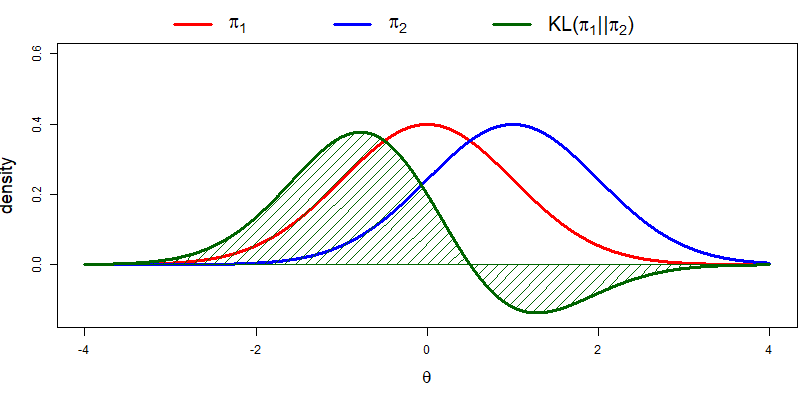
\includegraphics[width=0.9\linewidth]{figures/chapter_3/Figure1} 

}

\caption{KL divergences between two normal distributions. In this example, $\pi_1$ is a standard normal distribution and $\pi_2$ is a normal distribution with a mean of 1 and a variance of 1. The value of the KL divergence is equal to the integral over the parameter space for the function. The green shaded area above the x-axis adds to the KL divergence and the green shaded area below the x-axis subtracts from the KL divergence.}\label{fig:ch03fig1}
\end{figure}

\hypertarget{noninformativepriors}{%
\subsubsection{DAC}\label{noninformativepriors}}

The DAC, as mentioned before, is a ratio of two KL divergences. A KL divergence provides an indication of the discrepancy between two distributions. KL divergence does not, however,have a natural cut-off value or threshold that can help us decide when a certain amount of loss of information would constitute prior-data disagreement. To be able to objectively conclude when prior-data disagreement exists, the DAC compares the loss of information that a certain prior has with respect to the data with the loss of information that a benchmark prior has with respect to the data. The KL divergence between the chosen prior and the data is the numerator in the ratio whilst the KL divergence between some benchmark prior and the data is the denominator in the ratio. A benchmark prior, denoted by \(\pi^J(\theta)\), should be chosen such that the posterior distribution is completely dominated by the observed data \(\textbf{y}\) (Bernardo, \protect\hyperlink{ref-bernardo_reference_1979}{1979}). We denote such a posterior distribution by \(\pi^J(\theta|\textbf{y})\) and use this as a representation of the data.

\newpage

It is necessary to expand on the choice for the benchmark prior \(\pi^J(\theta)\) and in relation to this the posterior distribution \(\pi^J(\theta|\textbf{y})\). Bousquet (Bousquet, \protect\hyperlink{ref-bousquet_diagnostics_2008}{2008}) follows the reasoning Bernardo provided in discussion with Irony and Singpurwalla (Irony \& Singpurwalla, \protect\hyperlink{ref-irony_noninformative_1997}{1997}) to see \(\pi^J(\theta|\textbf{y})\) as a non-subjective posterior that is representative of the situation that one's prior knowledge was dominated by the data. In other words, \(\pi^J(\theta|\textbf{y})\) can be considered as a fictitious expert that is perfectly in agreement with the data, having no prior knowledge and being informed about the observations. \(\pi^J(\theta|\textbf{y})\) can be considered to be a reference posterior conveying the inferential content of the data (Bernardo, \protect\hyperlink{ref-bernardo_reference_1979}{1979}).

If \(\pi^J(\theta|\textbf{y})\) is taken to be a reference posterior, this would implicitly support the choice of \(\pi^J(\theta)\) such that it is a reference prior as originally developed by Bernardo (\protect\hyperlink{ref-bernardo_reference_1979}{1979}), further developed by Berger and Bernardo, e.g., (Berger \& Bernardo, \protect\hyperlink{ref-berger_estimating_1989}{1989}), described in Bernardo \& Smith (\protect\hyperlink{ref-bernardo_bayesian_1994}{1994}) and more formally worked out in Berger, Bernardo, \& Sun (\protect\hyperlink{ref-berger_formal_2009}{2009}). Reference priors are not the only possible choice for priors that convey in some sense minimal information or affect the information of the likelihood as weakly as possible (Gelman, Simpson, \& Betancourt, \protect\hyperlink{ref-gelman_prior_2017}{2017}). An extensive overview can be found in Kass \& Wasserman (\protect\hyperlink{ref-kass_selection_1996}{1996}) and some notable options are
Jeffrey's priors (Jeffreys, \protect\hyperlink{ref-jeffreys_invariant_1946}{1946}, \protect\hyperlink{ref-jeffreys_theory_1961}{1961}) and maximum entropy priors (Jaynes, \protect\hyperlink{ref-jaynes_rationale_1982}{1982}) to which the reference priors reduce in specific cases (Bernardo \& Smith, \protect\hyperlink{ref-bernardo_bayesian_1994}{1994}).

One notable problem for using reference priors as a choice for \(\pi^J(\theta)\) is that they often are improper priors (Yang \& Berger, \protect\hyperlink{ref-yang_catalog_1996}{1996}) and KL divergences and thus the DAC are not well defined when one of the distributions is improper. An adaptation of the DAC could be used, however a choice for a more convenient prior that is proper and leads to a posterior \(\pi^J(\theta|\textbf{y})\) closely resembling a reference posterior seems reasonable (Bousquet, \protect\hyperlink{ref-bousquet_diagnostics_2008}{2008}).

Now taking \(\pi^J(\theta|\textbf{y})\) as the reference posterior, \(\pi^J(\theta)\) as the benchmark prior and the data \(\textbf{y}\), the DAC for a chosen (expert) prior, denoted by \(\pi(\theta)\), can be expressed by

\begin{equation} 
DAC = \frac{KL[\pi^J(.|\textrm{y})||\pi]}{KL[\pi^J(.|\textrm{y})||\pi^J]},
\label{eq:ch03eq2}
\end{equation}
following the notation of Bousquet.

The benchmark, being an uninformative prior, should by definition not be conflicting with the data and therefore serves as a good reference point to determine if a certain amount of loss of information can be considered to be relevant. If a prior conflicts less with the data than the benchmark does, we should consider the prior to be in prior-data agreement. If a prior conflicts more with the data than the benchmark prior does, we do consider the prior to be in prior-data disagreement. Hence, if the DAC \textgreater{} 1, we conclude prior-data disagreement because the KL divergence of the prior is larger than the KL divergence of the benchmark prior; otherwise, we conclude prior-data agreement.

To illustrate the calculation of the DAC, we provide a numerical example together with a visual representation that can be found in Figure \ref{fig:ch03fig2}. Consider the case in which \(\pi^J(\theta|\textbf{y})\) is the \(N(0,1)\) density, \(\pi(\theta)\) is the \(N(0.5,1)\) density and \(\pi^J(\theta)\) is the \(N(0,900)\) density. The DAC is then calculated by taking the ratio of the following two KL divergences, Figure \ref{fig:ch03fig2}A; \(KL[\pi^J(.|\textrm{y})||\pi] = 0.125\) and Figure \ref{fig:ch03fig2}B; \(KL[\pi^J(.|\textrm{y})||\pi^J] = 2.902\), such that \(DAC = 0.125/2.902 = 0.043\). The DAC \textless{} 1, thus we conclude prior-data agreement, and \(\pi(\theta)\) is a better approximation of \(\pi^J(\theta|\textbf{y})\) than \(\pi^J(\theta)\).

\begin{figure}

{\centering \includegraphics[width=0.9\linewidth]{figures/chapter_3/Figure2} 

}

\caption{Calculating the DAC. In this example,  $\pi^J(\theta|\textbf{y})$ is a standard normal distribution,  $\pi(\theta)$ is a normal distribution with a mean of 0.5 and a variance of 1 and  $\pi^J(\theta)$ is a normal distribution with a mean of 0 and a variance of 900. The DAC < 1, thus prior-data agreement is concluded.}\label{fig:ch03fig2}
\end{figure}

\hypertarget{extension-to-multiple-experts}{%
\subsubsection{Extension to Multiple Experts}\label{extension-to-multiple-experts}}

The DAC, as described in the section above, determines the degree of prior-data (dis)agreement for a single prior that is to be evaluated. However, when we have multiple experts that each hold their own beliefs and we express each of these in the form of a probability distribution, we can ask some interesting questions. In Figure \ref{fig:ch03fig3}, we see some examples of situations that we could encounter. In Figure \ref{fig:ch03fig3}A, we see a situation in which experts differ in their predictions and their (un)certainty. The question that arises from the situation in Figure \ref{fig:ch03fig3}A is which of these predictions best approximates the information that the data provides us? Figure \ref{fig:ch03fig3}B shows a scenario in which the experts are predicting similar to each other but all differ with respect to the data. The question that arises from the situation in Figure \ref{fig:ch03fig3}B is which of the two is correct, the data or the experts?

To be able to answer these types of questions, we need to extend the DAC to incorporate multiple experts' priors, which are to be evaluated against the same posterior distribution, reflecting the data, and the same benchmark prior. The DAC thus needs to become a vector of length D resulting in

\begin{equation} 
DAC_d = \frac{KL[\pi^J(.|\textrm{y})||\pi_d]}{KL[\pi^J(.|\textrm{y})||\pi^J]},
\label{eq:ch03eq3}
\end{equation}
where the subscript \(d\) denotes the different input for \(D\) experts so \(DAC_d = DAC_1,...,DAC_D\) and \(\pi_d(\theta) = \pi_1(\theta),...\pi_D(\theta)\). This extension of the KL divergence in which not one but a vector of models are entered to be compared with the preferred model is straightforward and has previously been described in the context of the Akaike Information Criterion (AIC) (Akaike, \protect\hyperlink{ref-akaike_information_1973}{1973}; Burnham \& Anderson, \protect\hyperlink{ref-burnham_model_2002}{2002}).

\begin{figure}

{\centering 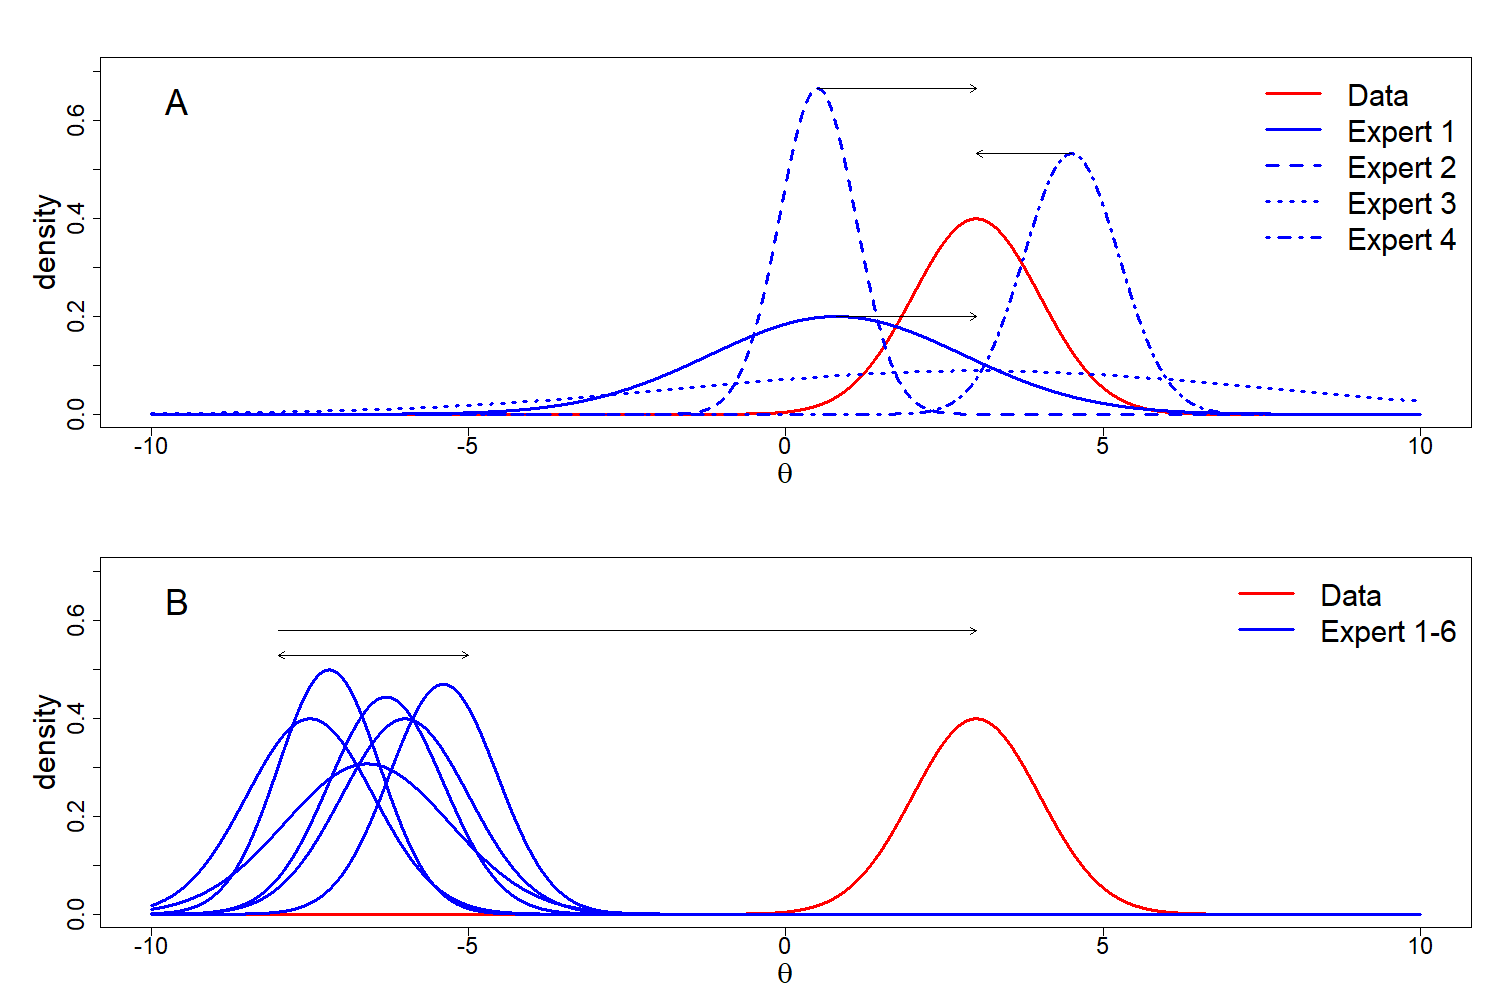
\includegraphics[width=0.9\linewidth]{figures/chapter_3/Figure3} 

}

\caption{Scenarios in which there are multiple experts and one source of data. (A) shows experts differing in prediction and (un)certainty, all (dis)agreeing to a certain extent with the data; (B) shows a scenario in which all experts disagree with the data, which results in the question of which of the sources of information is correct.}\label{fig:ch03fig3}
\end{figure}

\hypertarget{influence-of-the-benchmark}{%
\subsubsection{Influence of the Benchmark}\label{influence-of-the-benchmark}}

The choice for a specific benchmark can influence the results of the \(DAC_d\). Bousquet (\protect\hyperlink{ref-bousquet_diagnostics_2008}{2008}) suggests that, in applied studies, the availability of a convenient or intuitive prior for the benchmark seems reasonable. However, it is important to realize that the choice for a benchmark prior does influence the results of the analysis in the sense that the cut-off value for determining prior-data disagreement will shift as the KL divergence between \(\pi^J(\theta|\textrm{y})\) and \(\pi^J(\theta)\) changes. However, as long as the benchmark prior is an uninformative prior in the sense that the posterior distribution is dominated by the data, \(\pi^J(\theta|\textrm{y})\) will remain largely unchanged. This ensures that the \(DAC_d\) has the good property that when multiple experts are compared their ranking does not change dependent on which uninformative benchmark is chosen. This follows from the stability of \(\pi^J(\theta|\textrm{y})\), which ensures that the KL divergences between \(\pi^J(\theta|\textrm{y})\) and \(\pi^J(\theta)\) are stable. Different choices for \(\pi^J(\theta)\) do change the KL divergence in the denominator and therefore shift the prior-data disagreement boundary.

Concerning the benchmark, it is useful to note that the benchmark need not be restricted to an uninformative prior, but using an informative prior changes the interpretation and behavior of the DAC. When \(\pi^J(\theta)\) is informative, \(\pi^J(\theta|\textrm{y})\) is sensitive to the specification of \(\pi^J(\theta)\) and the KL divergence between \(\pi^J(\theta|\textrm{y})\) and \(\pi_d(\theta)\) need no longer be stable, potentially influencing the ranking of the experts. To show the above described behavior visually, we present the results of a simulation study in Figure \ref{fig:ch03fig4}. We show four different conditions, that is, four different choices for benchmark priors, to illustrate the change in behavior for the \(DAC_d\). In all four situations, we use the same data, \(\textbf{y}\), which is a sample of 100 from a standard normal distribution with a sample mean \(\bar{y}\). \(\pi_d(\theta)\) is the \(N(\mu_0, \sigma^2_0)\) density and we show the \(DAC_d\) values for \(\mu_0 = \bar{y}-4,...,\bar{y}+4\) and \(\sigma_0 = 0.1,...,3\). The four panels show different conditions for the benchmarks such that, in Figure \ref{fig:ch03fig4}A, it is the \(N(0, 10,000)\) density, in Figure \ref{fig:ch03fig4}B, the \(N(0, 1)\) density, in Figure \ref{fig:ch03fig4}C, the \(U(-50, 50)\) density and in Figure \ref{fig:ch03fig4}D the \(N(5, 0.5)\) density. It can be seen that, for the two uninformative priors in Figure \ref{fig:ch03fig4}A,C, the behavior of the \(DAC_d\) is stable. We would expect to draw the same conclusions and rank experts in the same way independent of the choice of either benchmark. However, when we specify an informative benchmark such as in Figure \ref{fig:ch03fig4}B,D, we see that both the behavior of the \(DAC_d\) and the determination of prior-data (dis)agreement shift. In Figure \ref{fig:ch03fig4}B, an informative and accurate benchmark leads almost invariably to concluding prior-data disagreement for \(\pi_d(\theta)\) In Figure \ref{fig:ch03fig4}D, the informative but inaccurate benchmark leads us to conclude prior-data disagreement only if \(\pi_d(\theta)\) is in the wrong location and has a very small variance.

The simulation study presented in Figure \ref{fig:ch03fig4} shows that the choice for a certain benchmark can influence your results, so, even if a convenient or intuitive prior seems reasonable, it should be carefully chosen. Researchers should be aware that their ranking is stable as long as an uninformative prior is chosen, but it might not be if the benchmark prior contains information.

\begin{figure}

{\centering 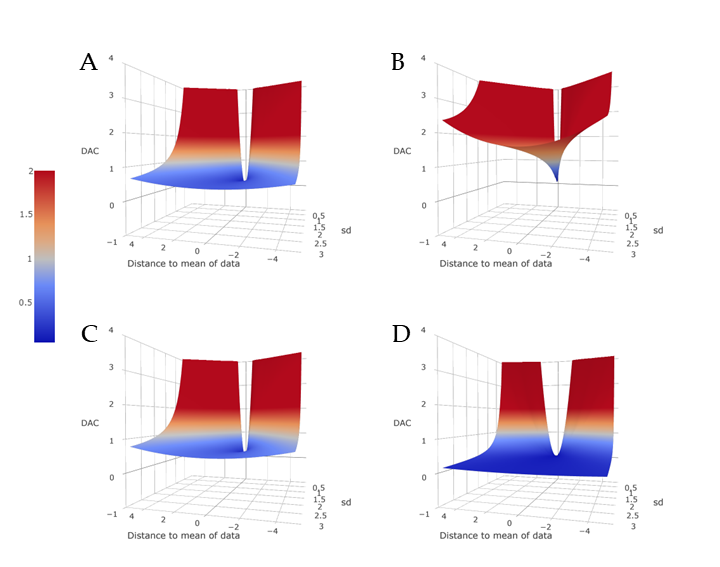
\includegraphics[width=0.9\linewidth]{figures/chapter_3/Figure4} 

}

\caption{The effect on the behavior of the $DAC_d$ for different choices for benchmark priors. All panels use the same data ($N = 100$) from a standard normal distribution and the same variations for $\pi_d(\theta)$ which are the normal distribution for which the parameters for the mean and standard deviation are given on the x-axis and y-axis of the panels. In (A), the benchmark is the $N(0, 10,000)$ density; in (B), the $N(0, 1)$ density; in (C), the $U(-50, 50)$ density and in (D), the $N(5, 0.5)$ density}\label{fig:ch03fig4}
\end{figure}

\hypertarget{DACvsBF}{%
\subsection{Comparison to Ranking by the Bayes Factor}\label{DACvsBF}}

In order to develop a good understanding of the behavior of the DAC for expert ranking, this section will provide a comparison to expert ranking using Bayes factors, that is, by ranking experts on the marginal likelihood resulting from their prior. First, we provide a mathematical description of the Bayes Factor (BF), which is a ratio of marginal likelihoods. Then, the influence of the benchmark prior will be discussed, followed by a comparison of expert ranking via Bayes Factors to expert ranking through the DAC.

\hypertarget{marginal-likelihood}{%
\subsubsection{Marginal Likelihood}\label{marginal-likelihood}}

For a model \(M\) and observed data \(\textbf{y}\), denote the likelihood \(f(\textbf{y}|\theta)\) and prior \(\pi(\theta)\) such that the posterior distribution

\begin{equation} 
\pi(\theta|\textbf{y}) = \frac{f(\textbf{y}|\theta)\pi(\theta)}{\int_{\Theta}f(\textbf{y}|\theta)\pi(\theta)d\theta}.
\label{eq:ch03eq4}
\end{equation}

The denominator on the right-hand side of Equation \eqref{eq:ch03eq4} is the marginal likelihood \(m(\textbf{y})\), sometimes called the evidence. The marginal likelihood can be thought of as the probability of the data averaged over the prior distribution (Liu \& Aitkin, \protect\hyperlink{ref-liu_bayes_2008}{2008}). As the probability of the data is dependent on the model, which is the set of probability distributions that is used (Wasserman, \protect\hyperlink{ref-wasserman_bayesian_2000}{2000}), the marginal likelihood is influenced by the choice of model \(M\), the data \(\textbf{y}\) and the prior \(\pi(\theta)\). If we have \(d\) experts and we keep \(M\) and \(\textbf{y}\) equal across experts, the only difference in \(m_d(\textbf{y})\) arises from the different specified priors \(\pi_d(\theta)\). We could thus differentiate between experts by assessing the probability of the data averaged across their specified prior beliefs.

\hypertarget{bayes-factor}{%
\subsubsection{Bayes Factor}\label{bayes-factor}}

The BF can be used to compare the marginal likelihoods for the different experts, \(m_d(\textbf{y})\), such that, for example,

\begin{equation} 
BF_{1d} = \frac{m_1(\textbf{y})}{m_d(\textbf{y})}
\label{eq:ch03eq5}
\end{equation}
provides the odds in favor of some model \(M_1\), versus model \(M_d\), the model that has the prior provided by expert \(d\). As the set of probability distributions that is used and the data \(\textbf{y}\) are the same between experts, this essentially provides the odds in favor of the prior \(\pi_1(\theta)\) versus prior \(\pi_d(\theta)\). Similarly, experts could be compared directly. It is well known that the BF is sensitive to the specification of different priors via the marginal likelihoods that are used (Kass \& Raftery, \protect\hyperlink{ref-kass_bayes_1995}{1995}; Liu \& Aitkin, \protect\hyperlink{ref-liu_bayes_2008}{2008}; Morey, Romeijn, \& Rouder, \protect\hyperlink{ref-morey_philosophy_2016}{2016}; Wasserman, \protect\hyperlink{ref-wasserman_bayesian_2000}{2000}). Liu and Aitkin (\protect\hyperlink{ref-liu_bayes_2008}{2008}) note that this is not necessarily undesirable. Moreover, in our case, this property is essential in allowing the evaluation of the relative merit of the experts' beliefs that are specified in the form of prior probability distributions.

\hypertarget{benchmark-model}{%
\subsubsection{Benchmark Model}\label{benchmark-model}}

The BF allows us to compare the odds in favor of one expert over another but neither the individual marginal likelihoods based on expert priors nor the ratios provide us with an assessment of the inherent appropriateness of the prior in terms of (dis)agreement between the prior and the data. As with the DAC, we could imagine taking a benchmark prior \(\pi^J(\theta)\) that serves as a reference point such that the marginal likelihood is \(m^J(\textbf{y})\). If we take

\begin{equation} 
BF_{Jd} = \frac{m^J(\textbf{y})}{m_d(\textbf{y})}
\label{eq:ch03eq6}
\end{equation}
and if \(BF_{Jd} < 1\), we would favor the model using the expert prior and conclude agreement with the data and, if \(BF_{Jd} > 1\), we would favor the model using the benchmark prior and conclude disagreement with the data.

However, we run into the same issue as with the KL divergences because the marginal likelihood is ill-defined if improper priors are used (Kass \& Raftery, \protect\hyperlink{ref-kass_bayes_1995}{1995}; Liu \& Aitkin, \protect\hyperlink{ref-liu_bayes_2008}{2008}; Wasserman, \protect\hyperlink{ref-wasserman_bayesian_2000}{2000}). Thus, again, reference priors (Bernardo, \protect\hyperlink{ref-bernardo_reference_1979}{1979}) are not suitable for use in this context. Raftery (\protect\hyperlink{ref-raftery_approximate_1996}{1996}) suggests using a reference set of proper priors and both Kass and Raftery (\protect\hyperlink{ref-kass_bayes_1995}{1995}) and Liu and Aitkin (\protect\hyperlink{ref-liu_bayes_2008}{2008}) suggest conducting a sensitivity analysis in any case. To keep the comparison between the \(BF_{Jd}\) and the \(DAC_d\) straightforward, we will use the same benchmark prior \(\pi^J(\theta)\) in both situations. As both \(BF_{Jd}\) and \(DAC_d\) are sensitive to the choice for \(\pi^J(\theta)\), a sensitivity analysis will be included in the empirical part of this paper. Note that this sensitivity is most evident when using these tools as a prior-data conflict criterion, as the expert rankings will generally remain unchanged for different uninformative benchmark priors.

\hypertarget{DACvsBF2}{%
\subsection{DAC Versus BF}\label{DACvsBF2}}

Burnham and Anderson state that the BF is analogous to the information-theoretic evidence ratio (\protect\hyperlink{ref-burnham_model_2002}{2002}), for instance, the DAC. If we directly compare two experts with a BF, we would obtain odds favoring one expert over another and if we compare the KL divergences between two experts, we could state that one expert has a certain amount of times the loss of information in relation to another. Despite the analogy, they are also inherently different. This is most clearly seen when we compare the alternative form of the DAC from Bousquet (\protect\hyperlink{ref-bousquet_diagnostics_2008}{2008}), which is given in our case by

\begin{equation} 
DAC_{2,d}^J = \frac{m^J(\textbf{y})}{m_d(\textbf{y})}exp\{KL[\pi^J(.|\textbf(y))||\pi_d(.|\textbf{y})]\} = BF_{Jd}exp\{KL[\pi^J(.|\textbf(y))||\pi_d(.|\textbf{y})]\}.
\label{eq:ch03eq7}
\end{equation}

Therefore, the difference between the DAC and BF can clearly be seen to be the fact that the DAC has an additional term which multiplies the BF by \(exp\{KL[\pi^J(.|\textbf{y})||\pi_d(.|\textbf{y})]\}\), the KL divergence between the reference posterior and the posterior from expert \(d\). This additional term is desirable, as it penalizes experts who are overly certain more harshly than the BF would.

To illustrate this, consider the following limiting case. Imagine an expert who believes that they are infinitely certain about the future. This expert should then specify their prior in the form of a Dirac delta function \(\delta_{\theta_0}(\theta)\), also called the degenerate distribution on the real line, which has density zero everywhere for \(\theta\) except for \(\theta_0\) where it has infinite density (Dirac, \protect\hyperlink{ref-dirac_principles_1947}{1947}). Moreover, the delta function actually integrates to one and in that sense is a proper prior which can also be viewed as an infinitely narrow Gaussian \(\delta(\theta-\theta_0) = \lim_{\sigma\to0}N(\theta|\theta_0, \sigma^2)\) (Barber, \protect\hyperlink{ref-barber_bayesian_2012}{2012}). Now, if an expert states their prior belief in the form of a delta function and \(\theta_0\) coincides with a region of \(\theta\) where the likelihood \(f(\textbf{y}|\theta)>0\), both the marginal likelihood and \(KL[\pi^J(.|\textbf{y})||\delta_{\theta_0}(.)]\) will become infinite. The meaning could, however, not differ any more. The marginal likelihood suggests that this expert is the best possible expert, whilst the KL divergence suggests that there is no worse expert. Although this scenario is quite extreme, van de Schoot, Griffioen and Winter (\protect\hyperlink{ref-van_de_schoot_dealing_2018}{2018}) did encounter such an expert in their elicitation endeavors.

\hypertarget{empirical-example}{%
\section{Empirical Example}\label{empirical-example}}

To show that the \(DAC_d\) can be used to evaluate and rank several experts based on their beliefs, we conducted an empirical study. The team that participated consisted of 11 experts, 10 regional directors and one director. All were eligible to be included in the study. Seven experts were randomly invited to participate in the research; if any of the selected experts did not want to participate, they were classified as not selected in the research. In this way, we avoided the possibility of group pressure to participate. In the end, four out of the seven selected experts participated in an elicitation. The experts (\(D = 4\)) provided forecasts concerning average turnover per professional in the first quarter of the year 2016. The (regional) directors are considered experts in knowledge concerning market opportunities, market dynamics and estimating the capabilities of the professionals to seize opportunities. Based on these skills, we expected that they could predict the average turnover per professional in the entire country in the first quarter of 2016. All information related to the empirical study can be found on the OSF webpage for this paper at \url{https://osf.io/u57qs}.

\hypertarget{elicitation-procedure}{%
\subsection{Elicitation Procedure}\label{elicitation-procedure}}

To get the experts to express their beliefs in the form of a probability distribution, we make use of the Five-Step Method (Veen, Stoel, Zondervan-Zwijnenburg, \& Schoot, \protect\hyperlink{ref-veen_proposal_2017}{2017}). To encapsulate the beliefs of the expert, the Five-Step Method actively separates two elements of the knowledge of the expert: tacit knowledge of the expert and their (un)certainty. In step one, a location parameter is elicited from the expert. This location parameter captures the tacit knowledge of the expert. To verify that the representation of the beliefs is accurate, step two is the incorporation of feedback implemented through the use of elicitation software. Experts can accept the representation of their beliefs or adjust their input. In step three, the (un)certainty of the experts is obtained and represented in the form of a scale and shape parameter. Step four is to provide feedback using elicitation software to verify the accurate representation of the expert's (un)certainty, which they can either accept or they can adjust their input until the representation is in accordance with their beliefs. The fifth step is to use the elicited expert's beliefs, in this case to determine their DAC score.

The experts first performed a practice elicitation for their own sales team before moving on to the whole country. The practice run enabled them to acquaint themselves with the elicitation procedure and software we used. The elicited distributions were restricted to be skewed normal distributions such that \(\pi_d(\theta)\) are \(SN(\mu_0,\sigma^2_0,\gamma_0)\) densities where subscript \(d\) denotes expert \(d = 1,...,D\), \(\mu_0\) denotes the prior mean, \(\sigma^2_0\) denotes the prior variance and \(\gamma_0\) denotes the prior skewness. The shape parameter \(\gamma_0\) is based on a general method for the transformation of symmetric distributions into skewed distributions as described by Equation (1) in Fernandez and Steel (\protect\hyperlink{ref-fernandez_bayesian_1998-1}{1998}). Table \ref{tab:ch03tab1} provides an overview of the elicited distributions for the four experts in this empirical study. The distributions are based upon transformed data to avoid revealing business-sensitive information.

\begin{longtable}[]{@{}lccc@{}}
\caption{\label{tab:ch03tab1} The values of the hyper parameters of \(\pi(\theta|y)\) for the empirical study.}\tabularnewline
\toprule
\begin{minipage}[b]{0.20\columnwidth}\raggedright
\strut
\end{minipage} & \begin{minipage}[b]{0.14\columnwidth}\centering
\(\mu_0\)\strut
\end{minipage} & \begin{minipage}[b]{0.16\columnwidth}\centering
\(\sigma_0\)\strut
\end{minipage} & \begin{minipage}[b]{0.16\columnwidth}\centering
\(\gamma_0\)\strut
\end{minipage}\tabularnewline
\midrule
\endfirsthead
\toprule
\begin{minipage}[b]{0.20\columnwidth}\raggedright
\strut
\end{minipage} & \begin{minipage}[b]{0.14\columnwidth}\centering
\(\mu_0\)\strut
\end{minipage} & \begin{minipage}[b]{0.16\columnwidth}\centering
\(\sigma_0\)\strut
\end{minipage} & \begin{minipage}[b]{0.16\columnwidth}\centering
\(\gamma_0\)\strut
\end{minipage}\tabularnewline
\midrule
\endhead
\begin{minipage}[t]{0.20\columnwidth}\raggedright
Expert 1\strut
\end{minipage} & \begin{minipage}[t]{0.14\columnwidth}\centering
2.15\strut
\end{minipage} & \begin{minipage}[t]{0.16\columnwidth}\centering
0.09\strut
\end{minipage} & \begin{minipage}[t]{0.16\columnwidth}\centering
0.78\strut
\end{minipage}\tabularnewline
\begin{minipage}[t]{0.20\columnwidth}\raggedright
Expert 2\strut
\end{minipage} & \begin{minipage}[t]{0.14\columnwidth}\centering
2.16\strut
\end{minipage} & \begin{minipage}[t]{0.16\columnwidth}\centering
0.07\strut
\end{minipage} & \begin{minipage}[t]{0.16\columnwidth}\centering
0.82\strut
\end{minipage}\tabularnewline
\begin{minipage}[t]{0.20\columnwidth}\raggedright
Expert 3\strut
\end{minipage} & \begin{minipage}[t]{0.14\columnwidth}\centering
1.97\strut
\end{minipage} & \begin{minipage}[t]{0.16\columnwidth}\centering
0.11\strut
\end{minipage} & \begin{minipage}[t]{0.16\columnwidth}\centering
0.82\strut
\end{minipage}\tabularnewline
\begin{minipage}[t]{0.20\columnwidth}\raggedright
Expert 4\strut
\end{minipage} & \begin{minipage}[t]{0.14\columnwidth}\centering
2.35\strut
\end{minipage} & \begin{minipage}[t]{0.16\columnwidth}\centering
0.11\strut
\end{minipage} & \begin{minipage}[t]{0.16\columnwidth}\centering
0.94\strut
\end{minipage}\tabularnewline
\bottomrule
\end{longtable}

\hypertarget{ranking-the-experts}{%
\subsection{Ranking the Experts}\label{ranking-the-experts}}

The predictions of the experts concerned the average turnover per professional (\(N = 104\)). The benchmark is the \(U(0, 5)\) density. A uniform distribution was chosen for the normal model in line with the prior used by Bousquet (\protect\hyperlink{ref-bousquet_diagnostics_2008}{2008}) in his Example 1 concerning a normal model. The lower bound of 0 arises out of the natural constraint that negative turnover will not occur, the upper bound of 5 was considered as a value that could not be attained, yet this number is to some extent arbitrary and a sensitivity analysis was conducted to investigate the impact of the choice for \(\pi^J(\theta)\). With regard to the desired minimal influence of \(\pi^J(\theta)\) on \(\pi^J(\theta|\textbf{y})\), in our case, the reference posterior can be analytically calculated (see Yang and Berger (\protect\hyperlink{ref-yang_catalog_1996}{1996})). The KL divergence for approximating the reference posterior with \(\pi^J(\theta|\textbf{y})\) was 0.00016, which we considered to be negligible.

We obtained the posterior distribution \(\pi^J(\theta|\textbf{y})\) using the rjags R-package (Plummer, \protect\hyperlink{ref-plummer_rjags:_2018}{2018}), such that \(\pi^J(\theta|\textbf{y})\) is the \(N(\mu_1,\sigma^2_1)\) density where \(\mu_1\) denotes the posterior mean and \(\sigma^2_1\) denotes the posterior variance. We used four chains of 25,000 samples after a burn-in period of 1000 samples per chain. Visual inspection and Gelman--Rubin diagnostics (Gelman \& Rubin, \protect\hyperlink{ref-gelman_inference_1992}{1992}) did not point towards problems with convergence of the chains and inspection of the autocorrelation plots showed no issues concerning autocorrelation. To compute the marginal likelihoods and BF, we used the R-Package rstan (Stan Development Team, \protect\hyperlink{ref-stan_development_team_rstan:_2018}{2018}\protect\hyperlink{ref-stan_development_team_rstan:_2018}{b}) with four chains of 1000 samples after burn-in to obtain the posterior distributions and we used the bridgesampling R-package (Gronau \& Singmann, \protect\hyperlink{ref-gronau_bridgesampling:_2017}{2017}) to obtain the marginal likelihoods and BF. For more details, see the data archive on the OSF webpage. Table \ref{tab:ch03tab2} displays KL divergences, \(DAC_d\) scores and ranking, marginal likelihoods and \(BF_{Jd}\) scores and ranking. Figure \ref{fig:ch03fig5} visually presents all relevant distributions concerning the empirical study. Figure \ref{fig:ch03fig6} panels A through E visually present all KL divergences from Table \ref{tab:ch03tab2}. Table \ref{tab:ch03tab3} presents the results for the sensitivity analysis for different choices for \(\pi^J(\theta)\) an and Table \ref{tab:ch03tab4} allows for a comparison between experts without reference to any benchmark \(\pi^J(\theta)\).

\begin{figure}

{\centering 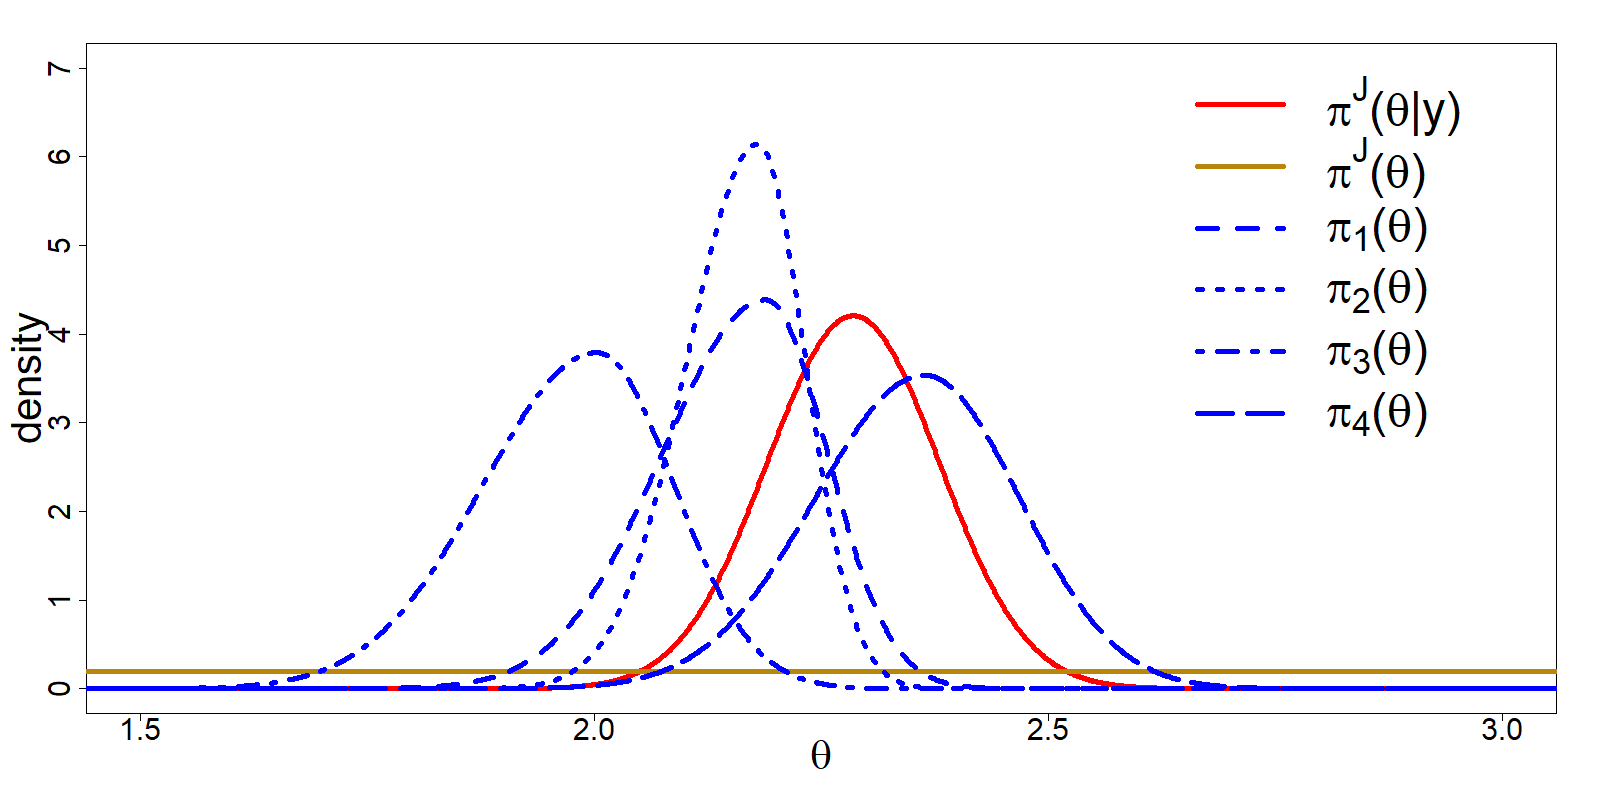
\includegraphics[width=0.9\linewidth]{figures/chapter_3/Figure5} 

}

\caption{Visual presentation of all relevant distributions for the empirical study; $\pi_d(\theta)$, $\pi^J(\theta)$ and $\pi^J(\theta|\textbf{y})$.}\label{fig:ch03fig5}
\end{figure}

The results of Table \ref{tab:ch03tab2} show that expert four provided the best prediction out of the experts, when using both the \(DAC_d\) and the \(BF_{Jd}\). Experts one and two provided similar predictions concerning their tacit knowledge; they expected almost the same value for the location parameter; however, expert one was less certain about this prediction (see Table \ref{tab:ch03tab1}). As the prediction of the location was not entirely correct, the increased uncertainty of expert one means that this expert provided more plausibility to the regions of the parameter space that were also supported by the data. Here we see the difference between \(DAC_d\) and the \(BF_{Jd}\) arise as discussed in section \ref{DACvsBF2}. Overconfidence is penalized more severely by the \(DAC_d\) and as such the conclusion on which expert would be preferred changes between experts one and two depending on which measure you use. When we look at the \(DAC_d\), in the case when \(\pi^J(\theta)\) is the \(U(0, 5)\) density, the additional penalization of the overconfidence even causes a different conclusion between experts one and two, namely, expert one is in prior-data agreement and expert two is in prior-data disagreement. For the \(BF_{Jd}\) both are concluded to be in agreement with the data. Expert three provided a prediction that, to a large extent, did not support the same parameter space as the data. In fact, expert three provides a lot of support for regions of the parameter space that the data did not support. The discrepancy between expert three and the data was of such proportions that, besides expert two, we also concluded a prior-data disagreement to exist for expert three. If we had no information beforehand, except knowing the region within which the average turnover per professional could fall, we would have lost less information than by considering the predictions of experts two and three. The \(BF_{Jd}\) differs from the \(DAC_d\) in the sense that when \(\pi^J(\theta)\) is the \(U(0, 5)\) density, the benchmark only outperforms expert 3.

\begin{figure}

{\centering 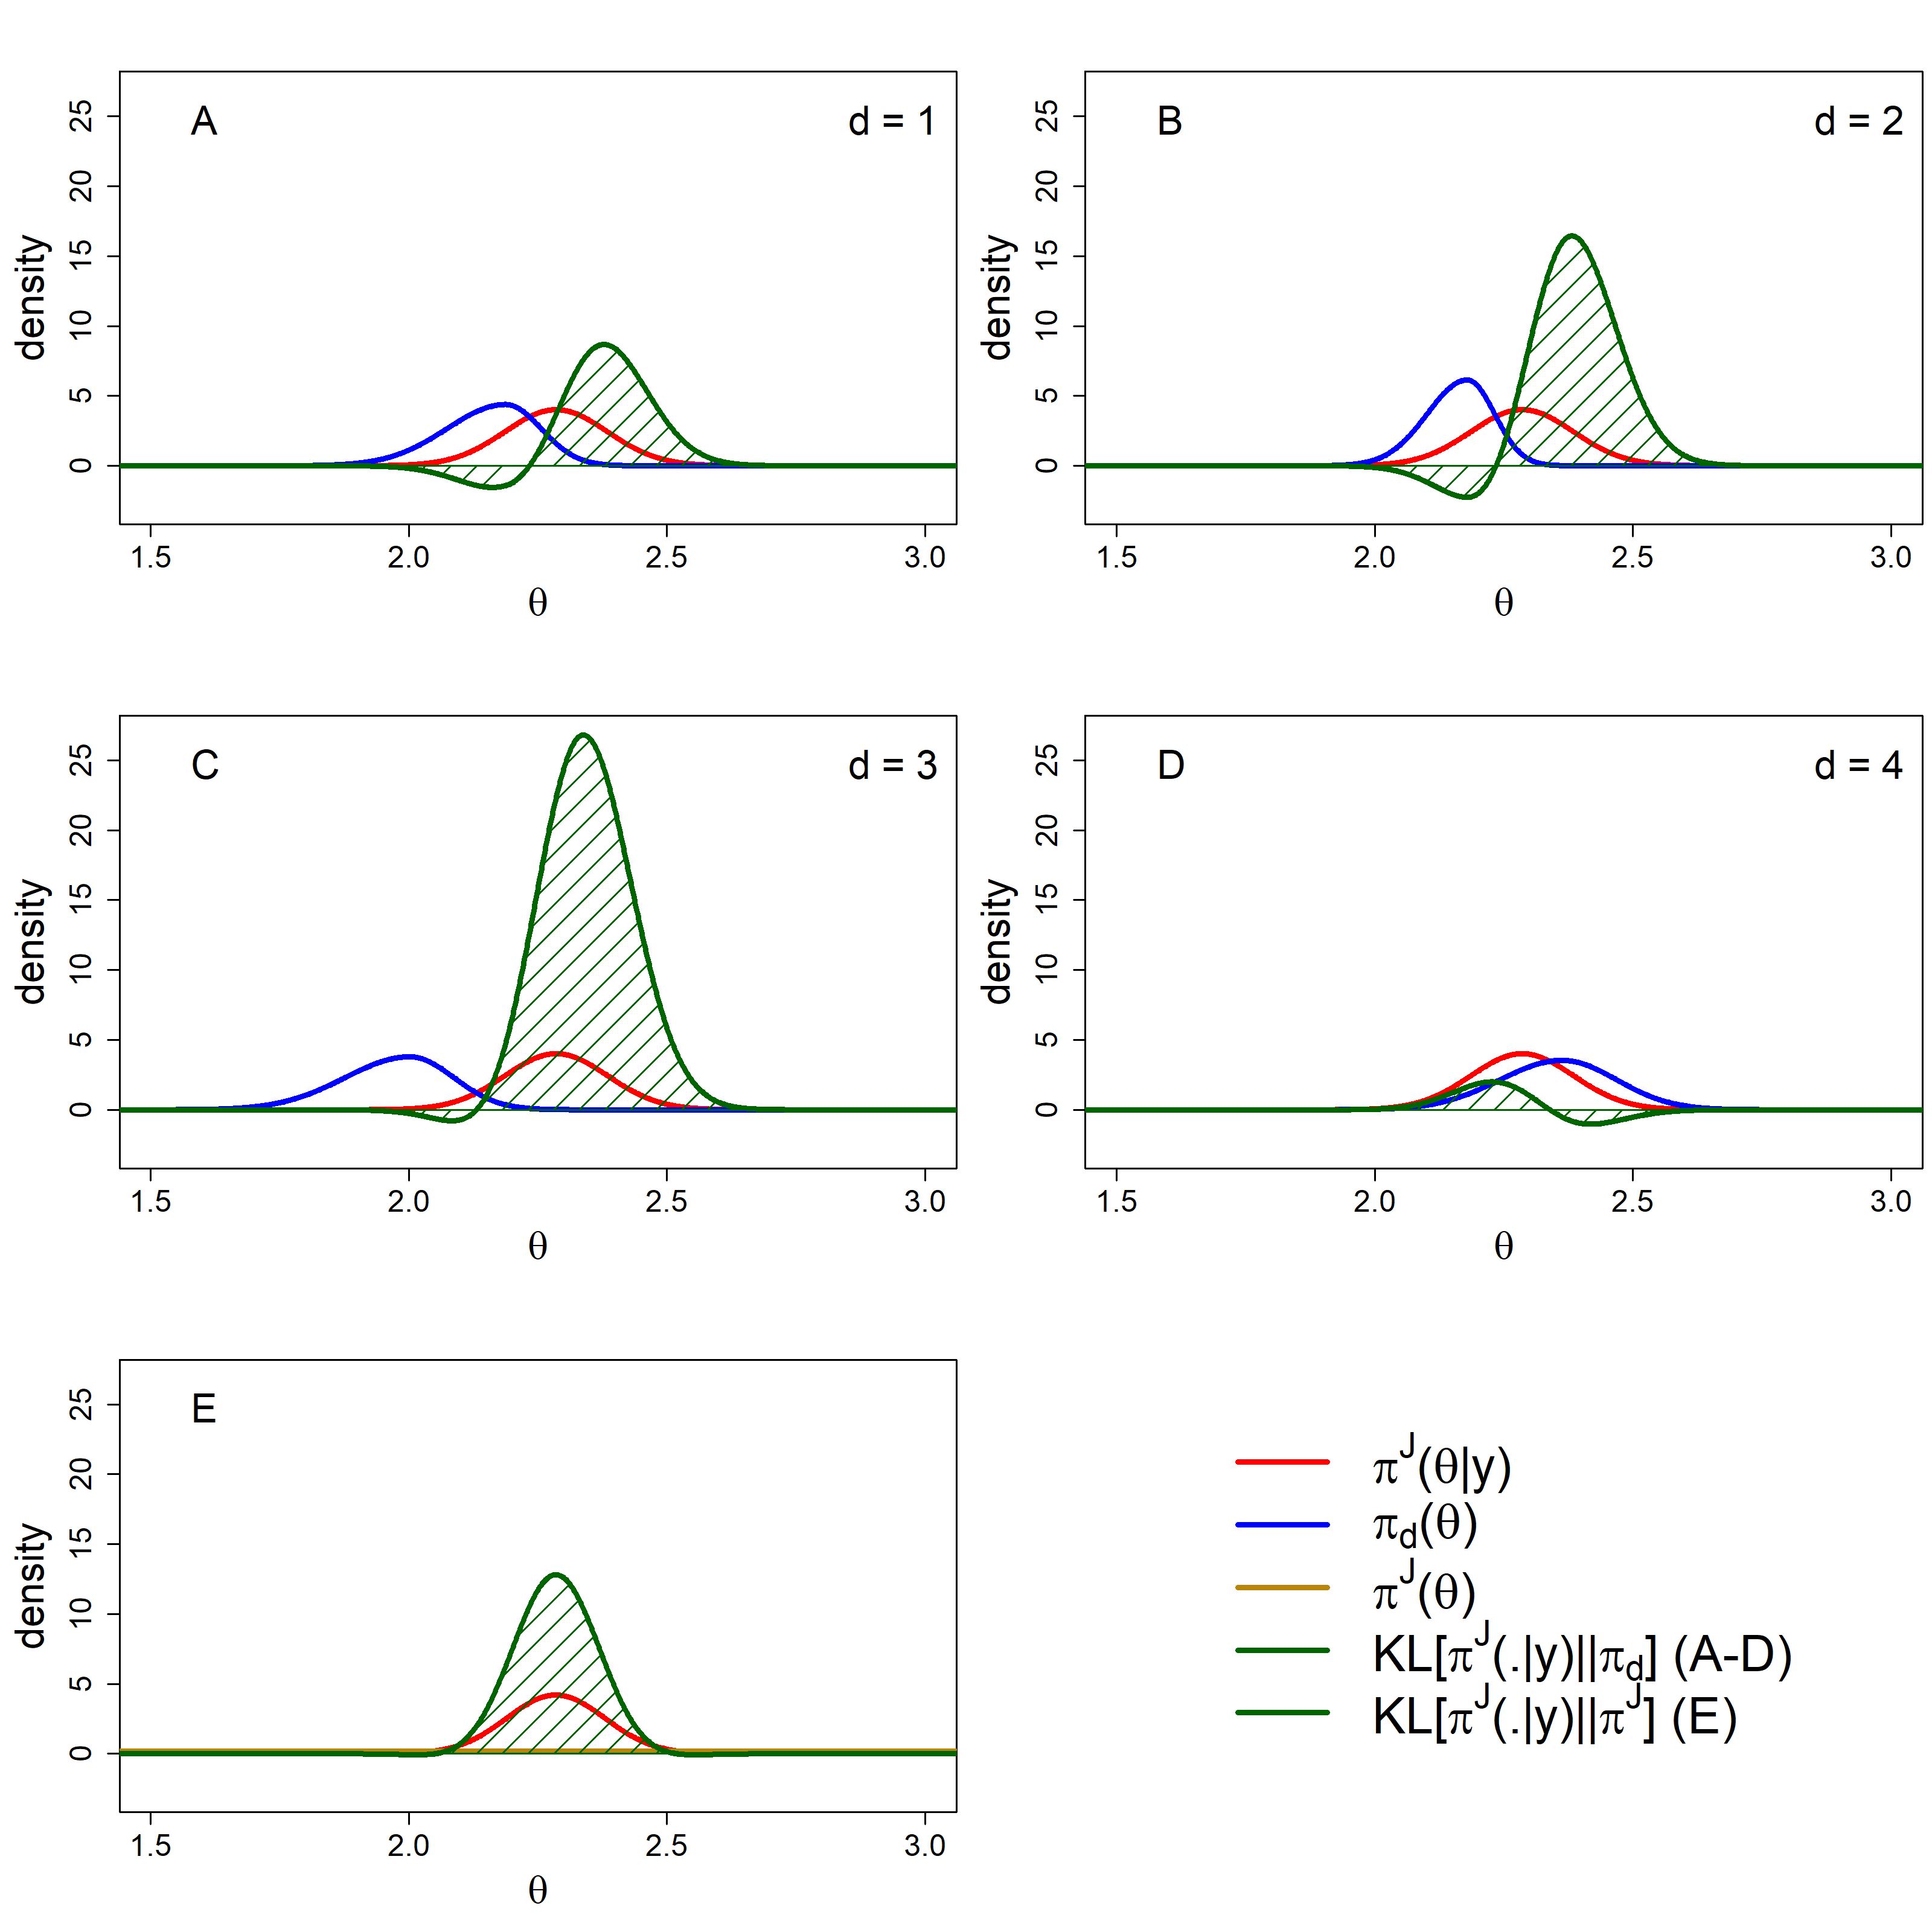
\includegraphics[width=0.9\linewidth]{figures/chapter_3/Figure6} 

}

\caption{All KL divergences for $\pi_d(\theta)$ (A–D) and $\pi^J(\theta)$ (E) with $\pi^J(\theta|\textbf{y})$ as the distribution that is to be approximated. (A) is for expert one; (B) for expert two; (C) for expert three and (D) for expert four.}\label{fig:ch03fig6}
\end{figure}

\newpage

\begin{longtable}[]{@{}lcccccc@{}}
\caption{\label{tab:ch03tab2} KL divergences, \(DAC_d\) scores and ranking, marginal likelihoods and \(BF_{Jd}\) scores and ranking, for the experts' priors and the benchmark prior. Note that marginal likelihoods are reported and not the log marginal likelihoods.}\tabularnewline
\toprule
\begin{minipage}[b]{0.11\columnwidth}\raggedright
\strut
\end{minipage} & \begin{minipage}[b]{0.12\columnwidth}\centering
KL Divergence\strut
\end{minipage} & \begin{minipage}[b]{0.08\columnwidth}\centering
\(DAC_d\)\strut
\end{minipage} & \begin{minipage}[b]{0.14\columnwidth}\centering
Ranking \(DAC_d\)\strut
\end{minipage} & \begin{minipage}[b]{0.16\columnwidth}\centering
\(m_d(\textbf{y})\) \&
\(m^J(\textbf{y})\)\strut
\end{minipage} & \begin{minipage}[b]{0.09\columnwidth}\centering
\(BF_{Jd}\)\strut
\end{minipage} & \begin{minipage}[b]{0.10\columnwidth}\centering
Ranking
\(BF_{Jd}\)\strut
\end{minipage}\tabularnewline
\midrule
\endfirsthead
\toprule
\begin{minipage}[b]{0.11\columnwidth}\raggedright
\strut
\end{minipage} & \begin{minipage}[b]{0.12\columnwidth}\centering
KL Divergence\strut
\end{minipage} & \begin{minipage}[b]{0.08\columnwidth}\centering
\(DAC_d\)\strut
\end{minipage} & \begin{minipage}[b]{0.14\columnwidth}\centering
Ranking \(DAC_d\)\strut
\end{minipage} & \begin{minipage}[b]{0.16\columnwidth}\centering
\(m_d(\textbf{y})\) \&
\(m^J(\textbf{y})\)\strut
\end{minipage} & \begin{minipage}[b]{0.09\columnwidth}\centering
\(BF_{Jd}\)\strut
\end{minipage} & \begin{minipage}[b]{0.10\columnwidth}\centering
Ranking
\(BF_{Jd}\)\strut
\end{minipage}\tabularnewline
\midrule
\endhead
\begin{minipage}[t]{0.11\columnwidth}\raggedright
Expert 1\strut
\end{minipage} & \begin{minipage}[t]{0.12\columnwidth}\centering
1.43\strut
\end{minipage} & \begin{minipage}[t]{0.08\columnwidth}\centering
0.56\strut
\end{minipage} & \begin{minipage}[t]{0.14\columnwidth}\centering
2\strut
\end{minipage} & \begin{minipage}[t]{0.16\columnwidth}\centering
5.57 x \(10^{-68}\)\strut
\end{minipage} & \begin{minipage}[t]{0.09\columnwidth}\centering
0.21\strut
\end{minipage} & \begin{minipage}[t]{0.10\columnwidth}\centering
3\strut
\end{minipage}\tabularnewline
\begin{minipage}[t]{0.11\columnwidth}\raggedright
Expert 2\strut
\end{minipage} & \begin{minipage}[t]{0.12\columnwidth}\centering
2.86\strut
\end{minipage} & \begin{minipage}[t]{0.08\columnwidth}\centering
1.12\strut
\end{minipage} & \begin{minipage}[t]{0.14\columnwidth}\centering
3\strut
\end{minipage} & \begin{minipage}[t]{0.16\columnwidth}\centering
6.82 x \(10^{-68}\)\strut
\end{minipage} & \begin{minipage}[t]{0.09\columnwidth}\centering
0.17\strut
\end{minipage} & \begin{minipage}[t]{0.10\columnwidth}\centering
2\strut
\end{minipage}\tabularnewline
\begin{minipage}[t]{0.11\columnwidth}\raggedright
Expert 3\strut
\end{minipage} & \begin{minipage}[t]{0.12\columnwidth}\centering
5.76\strut
\end{minipage} & \begin{minipage}[t]{0.08\columnwidth}\centering
2.26\strut
\end{minipage} & \begin{minipage}[t]{0.14\columnwidth}\centering
4\strut
\end{minipage} & \begin{minipage}[t]{0.16\columnwidth}\centering
2.19 x \(10^{-69}\)\strut
\end{minipage} & \begin{minipage}[t]{0.09\columnwidth}\centering
5.31\strut
\end{minipage} & \begin{minipage}[t]{0.10\columnwidth}\centering
4\strut
\end{minipage}\tabularnewline
\begin{minipage}[t]{0.11\columnwidth}\raggedright
Expert 4\strut
\end{minipage} & \begin{minipage}[t]{0.12\columnwidth}\centering
0.19\strut
\end{minipage} & \begin{minipage}[t]{0.08\columnwidth}\centering
0.07\strut
\end{minipage} & \begin{minipage}[t]{0.14\columnwidth}\centering
1\strut
\end{minipage} & \begin{minipage}[t]{0.16\columnwidth}\centering
1.72 x \(10^{-67}\)\strut
\end{minipage} & \begin{minipage}[t]{0.09\columnwidth}\centering
0.07\strut
\end{minipage} & \begin{minipage}[t]{0.10\columnwidth}\centering
1\strut
\end{minipage}\tabularnewline
\begin{minipage}[t]{0.11\columnwidth}\raggedright
Benchmark\strut
\end{minipage} & \begin{minipage}[t]{0.12\columnwidth}\centering
2.55\strut
\end{minipage} & \begin{minipage}[t]{0.08\columnwidth}\centering
--\strut
\end{minipage} & \begin{minipage}[t]{0.14\columnwidth}\centering
--\strut
\end{minipage} & \begin{minipage}[t]{0.16\columnwidth}\centering
1.16 x \(10^{-68}\)\strut
\end{minipage} & \begin{minipage}[t]{0.09\columnwidth}\centering
-\strut
\end{minipage} & \begin{minipage}[t]{0.10\columnwidth}\centering
-\strut
\end{minipage}\tabularnewline
\bottomrule
\end{longtable}

\vspace*{1cm}

\begin{longtable}[]{@{}lccccr@{}}
\caption{\label{tab:ch03tab3} Sensitivity analysis for different choices for \(\pi^J(\theta)\). Densities are given in the columns. The KL divergences and marginal likelihood \(m^J(\textbf{y})\) are presented in the rows. \(m_d(\textbf{y})\) do not change and are not reported.}\tabularnewline
\toprule
\begin{minipage}[b]{0.21\columnwidth}\raggedright
\strut
\end{minipage} & \begin{minipage}[b]{0.12\columnwidth}\centering
\(U(0,5)\)\strut
\end{minipage} & \begin{minipage}[b]{0.12\columnwidth}\centering
\(U(-10,10)\)\strut
\end{minipage} & \begin{minipage}[b]{0.12\columnwidth}\centering
\(N(0,10^2)\)\strut
\end{minipage} & \begin{minipage}[b]{0.13\columnwidth}\centering
\(N(0,10^3)\)\strut
\end{minipage} & \begin{minipage}[b]{0.13\columnwidth}\raggedleft
\(N(0,10^4)\)\strut
\end{minipage}\tabularnewline
\midrule
\endfirsthead
\toprule
\begin{minipage}[b]{0.21\columnwidth}\raggedright
\strut
\end{minipage} & \begin{minipage}[b]{0.12\columnwidth}\centering
\(U(0,5)\)\strut
\end{minipage} & \begin{minipage}[b]{0.12\columnwidth}\centering
\(U(-10,10)\)\strut
\end{minipage} & \begin{minipage}[b]{0.12\columnwidth}\centering
\(N(0,10^2)\)\strut
\end{minipage} & \begin{minipage}[b]{0.13\columnwidth}\centering
\(N(0,10^3)\)\strut
\end{minipage} & \begin{minipage}[b]{0.13\columnwidth}\raggedleft
\(N(0,10^4)\)\strut
\end{minipage}\tabularnewline
\midrule
\endhead
\begin{minipage}[t]{0.21\columnwidth}\raggedright
\(KL[\pi^J(.|\textbf{y})||\pi_1]\)\strut
\end{minipage} & \begin{minipage}[t]{0.12\columnwidth}\centering
1.43\strut
\end{minipage} & \begin{minipage}[t]{0.12\columnwidth}\centering
1.42\strut
\end{minipage} & \begin{minipage}[t]{0.12\columnwidth}\centering
1.37\strut
\end{minipage} & \begin{minipage}[t]{0.13\columnwidth}\centering
1.42\strut
\end{minipage} & \begin{minipage}[t]{0.13\columnwidth}\raggedleft
1.42\strut
\end{minipage}\tabularnewline
\begin{minipage}[t]{0.21\columnwidth}\raggedright
\(KL[\pi^J(.|\textbf{y})||\pi_2]\)\strut
\end{minipage} & \begin{minipage}[t]{0.12\columnwidth}\centering
2.86\strut
\end{minipage} & \begin{minipage}[t]{0.12\columnwidth}\centering
2.84\strut
\end{minipage} & \begin{minipage}[t]{0.12\columnwidth}\centering
2.75\strut
\end{minipage} & \begin{minipage}[t]{0.13\columnwidth}\centering
2.85\strut
\end{minipage} & \begin{minipage}[t]{0.13\columnwidth}\raggedleft
2.85\strut
\end{minipage}\tabularnewline
\begin{minipage}[t]{0.21\columnwidth}\raggedright
\(KL[\pi^J(.|\textbf{y})||\pi_3]\)\strut
\end{minipage} & \begin{minipage}[t]{0.12\columnwidth}\centering
5.76\strut
\end{minipage} & \begin{minipage}[t]{0.12\columnwidth}\centering
5.75\strut
\end{minipage} & \begin{minipage}[t]{0.12\columnwidth}\centering
5.67\strut
\end{minipage} & \begin{minipage}[t]{0.13\columnwidth}\centering
5.76\strut
\end{minipage} & \begin{minipage}[t]{0.13\columnwidth}\raggedleft
5.77\strut
\end{minipage}\tabularnewline
\begin{minipage}[t]{0.21\columnwidth}\raggedright
\(KL[\pi^J(.|\textbf{y})||\pi_4]\)\strut
\end{minipage} & \begin{minipage}[t]{0.12\columnwidth}\centering
0.19\strut
\end{minipage} & \begin{minipage}[t]{0.12\columnwidth}\centering
0.19\strut
\end{minipage} & \begin{minipage}[t]{0.12\columnwidth}\centering
0.20\strut
\end{minipage} & \begin{minipage}[t]{0.13\columnwidth}\centering
0.19\strut
\end{minipage} & \begin{minipage}[t]{0.13\columnwidth}\raggedleft
0.19\strut
\end{minipage}\tabularnewline
\begin{minipage}[t]{0.21\columnwidth}\raggedright
\(KL[\pi^J(.|\textbf{y})||\pi^J]\)\strut
\end{minipage} & \begin{minipage}[t]{0.12\columnwidth}\centering
2.55\strut
\end{minipage} & \begin{minipage}[t]{0.12\columnwidth}\centering
3.93\strut
\end{minipage} & \begin{minipage}[t]{0.12\columnwidth}\centering
4.18\strut
\end{minipage} & \begin{minipage}[t]{0.13\columnwidth}\centering
6.46\strut
\end{minipage} & \begin{minipage}[t]{0.13\columnwidth}\raggedleft
8.76\strut
\end{minipage}\tabularnewline
\begin{minipage}[t]{0.21\columnwidth}\raggedright
\(m^J(\textbf{y})\)\strut
\end{minipage} & \begin{minipage}[t]{0.12\columnwidth}\centering
1.16 x \(10^{-68}\)\strut
\end{minipage} & \begin{minipage}[t]{0.12\columnwidth}\centering
2.91 x \(10^{-69}\)\strut
\end{minipage} & \begin{minipage}[t]{0.12\columnwidth}\centering
5.65 x \(10^{-69}\)\strut
\end{minipage} & \begin{minipage}[t]{0.13\columnwidth}\centering
2.26 x \(10^{-69}\)\strut
\end{minipage} & \begin{minipage}[t]{0.13\columnwidth}\raggedleft
7.33 x \(10^{-70}\)\strut
\end{minipage}\tabularnewline
\bottomrule
\end{longtable}

\vspace*{1cm}

\begin{longtable}[]{@{}lclclclcl@{}}
\caption{\label{tab:ch03tab4} Comparison between experts based on KL divergences and marginal likelihoods. We report BF in favor of the row over the column and KL ratios for loss of information of the row over loss of information of the column.}\tabularnewline
\toprule
\begin{minipage}[b]{0.11\columnwidth}\raggedright
\strut
\end{minipage} & \begin{minipage}[b]{0.10\columnwidth}\centering
Expert 1\strut
\end{minipage} & \begin{minipage}[b]{0.06\columnwidth}\raggedright
\strut
\end{minipage} & \begin{minipage}[b]{0.11\columnwidth}\centering
Expert 2\strut
\end{minipage} & \begin{minipage}[b]{0.06\columnwidth}\raggedright
\strut
\end{minipage} & \begin{minipage}[b]{0.11\columnwidth}\centering
Expert 3\strut
\end{minipage} & \begin{minipage}[b]{0.07\columnwidth}\raggedright
\strut
\end{minipage} & \begin{minipage}[b]{0.10\columnwidth}\centering
Expert 4\strut
\end{minipage} & \begin{minipage}[b]{0.06\columnwidth}\raggedright
\strut
\end{minipage}\tabularnewline
\midrule
\endfirsthead
\toprule
\begin{minipage}[b]{0.11\columnwidth}\raggedright
\strut
\end{minipage} & \begin{minipage}[b]{0.10\columnwidth}\centering
Expert 1\strut
\end{minipage} & \begin{minipage}[b]{0.06\columnwidth}\raggedright
\strut
\end{minipage} & \begin{minipage}[b]{0.11\columnwidth}\centering
Expert 2\strut
\end{minipage} & \begin{minipage}[b]{0.06\columnwidth}\raggedright
\strut
\end{minipage} & \begin{minipage}[b]{0.11\columnwidth}\centering
Expert 3\strut
\end{minipage} & \begin{minipage}[b]{0.07\columnwidth}\raggedright
\strut
\end{minipage} & \begin{minipage}[b]{0.10\columnwidth}\centering
Expert 4\strut
\end{minipage} & \begin{minipage}[b]{0.06\columnwidth}\raggedright
\strut
\end{minipage}\tabularnewline
\midrule
\endhead
\begin{minipage}[t]{0.11\columnwidth}\raggedright
\strut
\end{minipage} & \begin{minipage}[t]{0.10\columnwidth}\centering
KL Ratio\strut
\end{minipage} & \begin{minipage}[t]{0.06\columnwidth}\raggedright
BF\strut
\end{minipage} & \begin{minipage}[t]{0.11\columnwidth}\centering
KL Ratio\strut
\end{minipage} & \begin{minipage}[t]{0.06\columnwidth}\raggedright
BF\strut
\end{minipage} & \begin{minipage}[t]{0.11\columnwidth}\centering
KL Ratio\strut
\end{minipage} & \begin{minipage}[t]{0.07\columnwidth}\raggedright
BF\strut
\end{minipage} & \begin{minipage}[t]{0.10\columnwidth}\centering
KL Ratio\strut
\end{minipage} & \begin{minipage}[t]{0.06\columnwidth}\raggedright
BF\strut
\end{minipage}\tabularnewline
\begin{minipage}[t]{0.11\columnwidth}\raggedright
Expert 1\strut
\end{minipage} & \begin{minipage}[t]{0.10\columnwidth}\centering
1\strut
\end{minipage} & \begin{minipage}[t]{0.06\columnwidth}\raggedright
1\strut
\end{minipage} & \begin{minipage}[t]{0.11\columnwidth}\centering
0.50\strut
\end{minipage} & \begin{minipage}[t]{0.06\columnwidth}\raggedright
0.82\strut
\end{minipage} & \begin{minipage}[t]{0.11\columnwidth}\centering
0.25\strut
\end{minipage} & \begin{minipage}[t]{0.07\columnwidth}\raggedright
25.42\strut
\end{minipage} & \begin{minipage}[t]{0.10\columnwidth}\centering
7.63\strut
\end{minipage} & \begin{minipage}[t]{0.06\columnwidth}\raggedright
0.32\strut
\end{minipage}\tabularnewline
\begin{minipage}[t]{0.11\columnwidth}\raggedright
Expert 2\strut
\end{minipage} & \begin{minipage}[t]{0.10\columnwidth}\centering
2.00\strut
\end{minipage} & \begin{minipage}[t]{0.06\columnwidth}\raggedright
1.22\strut
\end{minipage} & \begin{minipage}[t]{0.11\columnwidth}\centering
1\strut
\end{minipage} & \begin{minipage}[t]{0.06\columnwidth}\raggedright
1\strut
\end{minipage} & \begin{minipage}[t]{0.11\columnwidth}\centering
0.50\strut
\end{minipage} & \begin{minipage}[t]{0.07\columnwidth}\raggedright
31.13\strut
\end{minipage} & \begin{minipage}[t]{0.10\columnwidth}\centering
15.23\strut
\end{minipage} & \begin{minipage}[t]{0.06\columnwidth}\raggedright
0.40\strut
\end{minipage}\tabularnewline
\begin{minipage}[t]{0.11\columnwidth}\raggedright
Expert 3\strut
\end{minipage} & \begin{minipage}[t]{0.10\columnwidth}\centering
4.03\strut
\end{minipage} & \begin{minipage}[t]{0.06\columnwidth}\raggedright
0.04\strut
\end{minipage} & \begin{minipage}[t]{0.11\columnwidth}\centering
2.02\strut
\end{minipage} & \begin{minipage}[t]{0.06\columnwidth}\raggedright
0.03\strut
\end{minipage} & \begin{minipage}[t]{0.11\columnwidth}\centering
1\strut
\end{minipage} & \begin{minipage}[t]{0.07\columnwidth}\raggedright
1\strut
\end{minipage} & \begin{minipage}[t]{0.10\columnwidth}\centering
30.75\strut
\end{minipage} & \begin{minipage}[t]{0.06\columnwidth}\raggedright
0.01\strut
\end{minipage}\tabularnewline
\begin{minipage}[t]{0.11\columnwidth}\raggedright
Expert 4\strut
\end{minipage} & \begin{minipage}[t]{0.10\columnwidth}\centering
0.13\strut
\end{minipage} & \begin{minipage}[t]{0.06\columnwidth}\raggedright
3.09\strut
\end{minipage} & \begin{minipage}[t]{0.11\columnwidth}\centering
0.07\strut
\end{minipage} & \begin{minipage}[t]{0.06\columnwidth}\raggedright
2.52\strut
\end{minipage} & \begin{minipage}[t]{0.11\columnwidth}\centering
0.03\strut
\end{minipage} & \begin{minipage}[t]{0.07\columnwidth}\raggedright
78.54\strut
\end{minipage} & \begin{minipage}[t]{0.10\columnwidth}\centering
1\strut
\end{minipage} & \begin{minipage}[t]{0.06\columnwidth}\raggedright
1\strut
\end{minipage}\tabularnewline
\bottomrule
\end{longtable}

\newpage

From the sensitivity analyses of Table \ref{tab:ch03tab3} we can find that the reference posterior remains quite stable and therefore the KL divergences for the experts do not change substantially; however, the changing KL divergence for the benchmark would shift the prior-data disagreement boundary. When \(\pi^J(\theta)\) was the \(N(0,10^3)\) or \(N(0,10^4)\) density, expert three would no longer be in prior-data conflict, whilst prior-data disagreement for expert two was only concluded if \(\pi^J(\theta)\) was the \(U(0, 5)\) density. For the BF changing the benchmark also shifts the prior-data (dis)agreement boundary arbitrarily. In this case our decisions on prior-data (dis)agreement would only change for the \(N(0, 10^4)\) prior, where expert 4 would no longer be in prior-data disagreement. The sensitivity analysis showed that decisions on prior-data (dis)agreement might not be entirely reliable, whilst the ranking of experts remained stable.

Table \ref{tab:ch03tab4} shows the results when we only compare experts on their KL divergences and their marginal likelihoods and we omit the benchmarks. We see the difference between the BF and the KL divergence ratios when we compare experts one and two. The differences arise from the more severe penalization of overconfidence by KL divergences compared to BF, as discussed in section \ref{DACvsBF2}. Using KL divergence ratios we concluded that expert two had twice the amount of loss of information, whilst the BF even favors expert two over expert one with odds of 1.22

The results of the empirical study show a slight difference in the conclusions with regard to the ranking of the experts depending on which measure we used, \(DAC_d\) or \(BF_{Jd}\). Both measures select the same expert as being the best. If decisions should be made concerning average turnover per professional, decision makers would be wise to consult expert four, as this expert seemed to have the best knowledge of the underlying factors driving these results.

\hypertarget{ch03discussion}{%
\section{Discussion}\label{ch03discussion}}

In this paper, we use both the BF and the DAC to rank experts' beliefs when they are specified in the probabilistic form of prior distributions. When comparing the BF and the DAC, the limiting case example of Section \protect\hyperlink{DACvsBF2}{3.2.3} springs to mind. In the introduction, we stated that forecasting without specifying uncertainty would not make sense to us and, in that light, we would prefer to use a measure that would classify doing so as undesirable behavior and punish this extreme case. An example of this behavior can be seen in the empirical example where while using the BF we would favor expert two over expert one, however whilst using KL divergences, we would favor expert one over expert two.

The sensitivity analysis in the empirical example, however, also highlighted some undesirable characteristics of the DAC for our context, namely the sensitivity to different choices for \(\pi^J(\theta)\). In the context of ranking experts, it can make sense to drop the association between \(\pi^J(\theta)\) and \(\pi^J(\theta|\textbf{y})\). \(\pi^J(\theta|\textbf{y})\) can remain a reference posterior and as such represent the characteristics of \(\textbf{y}\). \(\pi^J(\theta)\) can either be omitted or be specified such that it is meaningful. If \(\pi^J(\theta)\) is omitted, we do not have a reference point for (dis)agreement; however, if arbitrarily chosen benchmarks shift this reference point, it hardly has any meaning. Without a benchmark, experts can still be compared with each other in terms of ratios of loss of information, as presented in Table \ref{tab:ch03tab4}. However, if \(\pi^J(\theta)\) is meaningful, one could imagine, for instance, a gold standard that is used in a forecasting situation; we can assess experts' beliefs in relation to this meaningful benchmark and see if they outperform this benchmark. If the association between \(\pi^J(\theta)\) and \(\pi^J(\theta|\textbf{y})\) is dropped, we can specify informative benchmarks without the adverse effects of changing \(\pi^J(\theta|\textbf{y})\) and thereby the divergences between \(\pi^J(\theta|\textbf{y})\) and \(\pi_d(\theta)\). Moreover, specifying informative benchmarks requires elaboration of the rationale behind the choice, thus enhancing trust in the conclusions if a sensitivity analysis shows different priors representing similar information that leads us to the same conclusions.

One of the reasons for the sensitivity of the DAC to different choices for \(\pi^J(\theta)\) can be seen by comparing the KL divergences of expert one and two of the empirical example. As a referee pointed out to us, KL divergences are tail sensitive and this can be seen in this comparison. Expert one is a little more uncertain and as such the tail of \(\pi_1(\theta)\) overlaps somewhat more with \(\pi^J(\theta|\textbf{y})\) than the tails of \(\pi_2(\theta)\). This leads to half the loss of information. One could deem this tail sensitivity to be undesirable and, with differently shaped prior distributions, this problem might become more pronounced. If it is deemed undesirable, one could favor using the BF, which actually favors expert two with odds of 1.22 over expert 1. Alternatively, an interesting area for future research could be to investigate the use of alternative divergence measures. A good starting point for finding alternative measures can be found in the Encyclopedia of Distances by Deza and Deza (\protect\hyperlink{ref-deza_encyclopedia_2009}{2009}).

In the current paper, we followed Bousquet (\protect\hyperlink{ref-bousquet_diagnostics_2008}{2008}) and used KL divergences and this raises two important methodological issues; see Burnham and Anderson (\protect\hyperlink{ref-burnham_model_2002}{2002}) for an elaborated discussion. First, the reference model should be known. Second, the parameters should be known for the model that is evaluated, i.e., the formalized expert prior. The issues make the KL divergence a measure that, according to some, for instance Burnham and Anderson (\protect\hyperlink{ref-burnham_model_2002}{2002}), cannot be used for real world problems and previously led to the development of the AIC (Akaike, \protect\hyperlink{ref-akaike_information_1973}{1973}), which uses the relative expected KL divergence. The AIC deals with the two issues by taking the reference model as a constant in comparing multiple models and using the maximum likelihood estimates for the parameters of the models to be evaluated, introducing a penalty term for the bias that this induces.

We conclude that we can use the KL divergence in the context of the DACd and with the following reasoning. We define \(\pi^J(\theta|\textbf{y})\) to be the reference distribution as it reflects a fictional expert that is completely informed by the data and thus it is known. In the case of the empirical example, the data is even the true state of affairs, i.e., the actual realizations of the turnover for each professional. Concerning the parameter for the models to be evaluated, \(\pi_d(\theta)\) should reflect the exact beliefs of the experts. We use the Five-Step Method (Veen et al., \protect\hyperlink{ref-veen_proposal_2017}{2017}) which incorporates feedback at each stage of the elicitation, ensuring that experts confirm that their beliefs are accurately represented by the location, shape and scale parameters. We acknowledge that whether the parameters represent exactly an expert's beliefs cannot be known, but we feel confident that the procedure we use at least aims to obtain very accurate representations. As experts can continue to adapt their input until they are satisfied with the representation of their beliefs, this should overcome problems with the second issue.

While we use \(\pi^J(\theta|\textbf{y})\), and thus know the reference distribution, and we firmly believe that we properly represent the experts' beliefs, it seems highly implausible that a DAC score of 0 can be attained. It is unlikely that, in predicting future events, one estimates precisely the optimal location and exactly the optimal amount of uncertainty.

Although a priori specification of optimal uncertainty is unlikely, we are able to gain an indication of the appropriate amount of uncertainty a posteriori. \(\pi^J(\theta|\textbf{y})\) provides an excellent indication of the appropriate uncertainty. Given that one had no knowledge beforehand and is rationally guided by the data, following probabilistic reasoning, one arrives at the posterior belief represented by \(\pi^J(\theta|\textbf{y})\) (Bousquet, \protect\hyperlink{ref-bousquet_diagnostics_2008}{2008}; Irony \& Singpurwalla, \protect\hyperlink{ref-irony_noninformative_1997}{1997}). The posterior described the range of values that would have been plausible given this information. This indication is, however, conditional on the fact that the data provide an accurate representation of the state of affairs.

Given that we can attain information on the expected value for the parameter of interest, the appropriate amount of uncertainty and the quality of the approximation by each expert, we can start a learning process. By sharing the reasons behind the choices they made, experts can learn from one another as evidence shows which reasoning leads to the most accurate predictions. The data can inform the experts so that they can adjust their estimates and uncertainty. Through this evaluation, expertise can increase and in the long run convergence should be reached between both different experts' predictions and between the experts and the data. When this convergence is reached, this indicates that at least part of the epistemic uncertainty is eliminated and we have a better understanding of the data generating processes and are better able to make an informed decision. Note that, if we wish to incorporate the relevant factors that are identified by the experts, these should be included in the model so that part of the posterior uncertainty about our parameter can be explained. The explained variance can be seen as a reduction of the epistemic uncertainty or learning effect.

In the empirical example, we can already see some opportunities for learning. For example, expert three misestimated the location of the parameter, which indicates, at least to some extent, faulty or missing tacit knowledge. By starting a dialogue with the other experts, he or she could learn why they all estimated the average turnover per professional to be higher. Expert one and two had almost identical predictions concerning the location, but expert one expressed more uncertainty. Perhaps this indicated more acknowledgement of epistemic uncertainty; a dialogue could shed more light on the differences in choices of expert one and two. Our empirical example contains just four experts, but the methods used are easily scalable to include more experts, with only additional elicitation efforts required. Including more experts can result in more opportunities for learning.

Concerning the appropriateness of the ranking that is obtained using the \(DAC_d\), we have the following to add. One could argue that perhaps the sample entails extreme data. However, even if this is true, the experts should have considered the data to be plausible, for it did occur. Thus, if an expert exhibits large KL divergence with \(\pi^J(\theta|\textbf{y})\), this expert simply did not expect that these data were likely or plausible. By incorporating (un)certainty in the evaluation, the \(DAC_d\), or KL divergences if a benchmark is omitted, produces the required behavior to fairly compare experts' beliefs. Given that it is appropriate to take uncertainty into account, a prior can be over-specific such that it does not adhere to the principles underlying the data generating mechanism. KL divergences reward the specification of an appropriate amount of uncertainty and penalize overconfidence.

\newpage

To conclude this discussion, we state recommendations for researchers facing similar problems:

\begin{itemize}
\tightlist
\item
  Use \(DAC_d\) instead of BF.
\item
  Specify \(\pi^J(\theta|\textbf{y})\) such that it serves as a reference posterior and drop the association between \(\pi^J(\theta|\textbf{y})\) and \(\pi^J(\theta)\).
\item
  Consider whether a meaningful benchmark can be determined. If not, only use \(KL[\pi^J(.|\textbf{y})||\pi_d]\) and compare experts with each other and not with a benchmark.
\item
  Carrying out a sensitivity analysis is always recommendable, even more so if benchmarks are used.
\end{itemize}

\hypertarget{ch03ethics}{%
\section*{Ethics Statement}\label{ch03ethics}}
\addcontentsline{toc}{section}{Ethics Statement}

This study was carried out in accordance with the recommendations of the internal Ethics Committee of the Faculty of Social and Behavioural Sciences of Utrecht University, with written informed consent from all subjects. All subjects gave written informed consent in accordance with the Declaration of Helsinki. The protocol was approved by the internal Ethics Committee of the Faculty of Social and Behavioural Sciences of Utrecht University.

\hypertarget{ch03funding}{%
\section*{Funding}\label{ch03funding}}
\addcontentsline{toc}{section}{Funding}

The project was supported by the Netherlands Organization for Scientific Research grant number NWO-VIDI-452-14-006. K.M. was supported by the Netherlands Organization for Scientific Research grant number NWO-452-12-010.

\hypertarget{ch03acknowledgments}{%
\section*{Acknowledgments}\label{ch03acknowledgments}}
\addcontentsline{toc}{section}{Acknowledgments}

We are grateful to all participants of the empirical study for their time, energy and predictions. In addition, we would like to thank the company for allowing us access to their resources and information, thereby enabling us to provide empirical support for the theoretical work. We would also like to thank the anonymous reviewers whose comments and suggestions greatly improved the manuscript.

\hypertarget{ch03conflict}{%
\section*{Conflicts of Interest Statement}\label{ch03conflict}}
\addcontentsline{toc}{section}{Conflicts of Interest Statement}

The authors declare that the research was conducted in the absence of any commercial or financial relationships that could be construed as a potential conflict of interest.

\hypertarget{Hierarchical}{%
\chapter{A Step Forward: Bayesian Hierarchical Modelling as a Tool in Assessment of Individual Discrimination Performance}\label{Hierarchical}}

\chaptermark{A STEP FORWARD}
\thispagestyle{empty}

\blfootnote{This chapter is published as de Klerk, M., Veen, D., Wijnen, F. \& de Bree, E. (2019). A Step Forward: Bayesian Hierarchical Modelling as a Tool in Assessment of Individual Discrimination Performance. \textit{Infant Behavior and Development}., 57, 101345. Doi: 10.1016/j.infbeh.2019.101345 \\
\indent EdB, MdK and FW designed the study. MdK conducted the group level analysis. DV conducted the individual level analyses. MdK wrote and revised the paper with input and feedback from EdB, DV and FW. DV wrote and revised the text concerning the Bayesian Analyses with input and feedback by EdB, MdK and FW.}

\hypertarget{abstract-2}{%
\section*{Abstract}\label{abstract-2}}
\addcontentsline{toc}{section}{Abstract}

\small

Individual assessment of infants' speech discrimination is of great value for studies of language development that seek to relate early and later skills, as well as for clinical work. The present study explored the applicability of the hybrid visual fixation paradigm (Houston et al., \protect\hyperlink{ref-houston_assessing_2007}{2007}) and the associated statistical analysis approach to assess individual discrimination of a native vowel contrast, /a:/ - /e:/, in Dutch 6 to 10-month-old infants. Houston et al.~found that 80\% (8/10) of the 9-month-old infants successfully discriminated the contrast between pseudowords boodup - seepug. Using the same approach, we found that 12\% (14/117) of the infants in our sample discriminated the highly salient /a:/ - /e:/ contrast. This percentage was reduced to 3\% (3/117) when we corrected for multiple testing. Bayesian hierarchical modeling indicated that 50\% of the infants showed evidence of discrimination. Advantages of Bayesian hierarchical modeling are that 1) there is no need for a correction for multiple testing and 2) better estimates at the individual level are obtained. Thus, individual speech discrimination can be more accurately assessed using state of the art statistical approaches.

\normalsize
\newpage

\hypertarget{ch04introduction}{%
\section{Introduction}\label{ch04introduction}}

Early speech discrimination is assumed to be vital for children's language acquisition, as it is a first step into the formation of speech sound categories. These, in turn, are necessary for word learning (e.g.~Tsao, Liu, \& Kuhl, \protect\hyperlink{ref-tsao_speech_2004}{2004}). These past decades have seen a significant increase in our understanding of the development of speech perception in infants (see for recent reviews Maurer \& Werker, \protect\hyperlink{ref-maurer_perceptual_2014}{2014}; Tsuji \& Cristia, \protect\hyperlink{ref-tsuji_perceptual_2014}{2014}). However, the majority of studies have based their conclusions on group data. It has thus far turned out difficult to make claims about individual performance and development, even though this type of information is critical for understanding individual developmental trajectories as well as clinical questions. It seems that only one study has addressed this matter so far (Houston et al., \protect\hyperlink{ref-houston_assessing_2007}{2007}). In the present study, we use a variant of Houston et al.'s hybrid visual fixation paradigm (HVF), and we describe and evaluate a new approach for assessing individual infants' phoneme discrimination.

Infant speech discrimination can only be measured indirectly. A frequently used behavioral method is a habituation paradigm. In such paradigms, looking time is the preferred dependent variable. Generally, in habituation paradigms infants are habituated on a set of stimuli (A), followed by a test phase in which infants are tested on new set of stimuli (B), i.e., the `dishabituation' or `change' trials. If infants are sensitive to the difference between A and B, longer listening times are expected to the novel stimuli (B) (Sokolov, \protect\hyperlink{ref-sokolov_perception_1963}{1963}). Studies often employ designs with only 2-4 test trials, see Colombo \& Mitchell (\protect\hyperlink{ref-colombo_infant_2009}{2009}) for a review. This can lead to interpretation difficulties, because infant data is, without exception, noisy. Group results often show large individual variation in looking times. This reflects substantial interindividual variation, comprising overall long or short lookers. It also reflects intra-individual variation. This variation may result from a variety of factors, both infant-internal, such as gas in the digestive system, tiredness, developmental level, memory capacity, attentiveness, motivation, and external factors, such as sounds other than the stimuli, stimulus complexity, and task demands. Hence, the length of a look does not merely reflect the mental processing of the stimulus, and thus does not unequivocally mirror habituation or dishabituation (Oakes, \protect\hyperlink{ref-oakes_using_2010}{2010}). In order to deal with the noise, researchers typically collapse data over individuals. However, the HVF paradigm (Houston et al., \protect\hyperlink{ref-houston_assessing_2007}{2007}) uses 14 test trials instead of 2-4 test trials, which in principle allows for individual assessment, as the higher number of test trials will boost the signal-to-noise ratio.

Recently, there has been a growing interest in explaining individual differences in infants' early speech perception, i.e.~word segmentation and speech sound discrimination skills, see Cristia, Seidl, Junge, Soderstrom, \& Hagoort (\protect\hyperlink{ref-cristia_predicting_2014}{2014}) for a review. A frequently used approach to individual differences is to use follow-up data, such as later vocabulary size, reading scores or other skills to predict (in retrospect) infants' looking times (e.g.~Altvater-Mackensen \& Grossmann, \protect\hyperlink{ref-altvater-mackensen_learning_2015}{2015}; Cristia, \protect\hyperlink{ref-cristia_fine-grained_2011}{2011}; Junge \& Cutler, \protect\hyperlink{ref-junge_early_2014}{2014}; Melvin et al., \protect\hyperlink{ref-melvin_home_2017}{2017}; Molfese, \protect\hyperlink{ref-molfese_predicting_2000}{2000}; Newman, Ratner, Jusczyk, Jusczyk, \& Dow, \protect\hyperlink{ref-newman_infants_2006}{2006}). For instance, Newman et al. (\protect\hyperlink{ref-newman_infants_2006}{2006}) found that 24-month-old toddlers with larger vocabulary sizes were better at speech perception tasks in infancy than their peers with smaller vocabularies. Although the reported correlations between looking time data and later language, cognitive or social measures, e.g.~vocabulary size, social interaction, social economic status (e.g.~Altvater-Mackensen \& Grossmann, \protect\hyperlink{ref-altvater-mackensen_learning_2015}{2015}) are sometimes low to moderate, the meta-analysis of Cristia et al. (\protect\hyperlink{ref-cristia_predicting_2014}{2014}) shows that early speech perception skills have a predictive value of later language skills.

Even though there is a (weak) positive relation between early looking time data and later language, cognitive or social measures, this is not the same as being able to assess an individual child's ability to discriminate speech sounds or segment words. There are three reasons why individual data collected with the traditional discrimination paradigms cannot provide this information. First, individual data is likely to show that some infants have, on average, longer listening times to the familiarized, than to the new stimuli (Houston-Price \& Nakai, \protect\hyperlink{ref-houston-price_distinguishing_2004}{2004}). This could be due to some infants having reached the habituation criterion without having fully encoded the stimulus (Aslin \& Fiser, \protect\hyperlink{ref-aslin_methodological_2005}{2005}); as a consequence they do not look longer to the new stimulus. However, such a looking pattern does not imply that they cannot discriminate A from B (e.g.~Aslin \& Fiser, \protect\hyperlink{ref-aslin_methodological_2005}{2005}; Houston-Price \& Nakai, \protect\hyperlink{ref-houston-price_distinguishing_2004}{2004}). This implies that the direction of the difference in raw looking times cannot be used to infer discrimination. Second, it is not a priori clear that a larger looking time difference between stimuli A and B is evidence for better discrimination performance, and a smaller difference reflects poorer discrimination (Aslin \& Fiser, \protect\hyperlink{ref-aslin_methodological_2005}{2005}), because there is no clear conceptualization of looking time duration and discrimination. Third, although Houston found high test-retest reliability (Houston et al., \protect\hyperlink{ref-houston_assessing_2007}{2007}), this test-retest reliability was found to be extremely variable across different experiments in a multi-center study by Cristia, Seidl, Singh, \& Houston (\protect\hyperlink{ref-cristia_test-retest_2016}{2016}). Across the three participating labs 12 speech perception experiments were conducted, which included testing and retesting of 5-12-month-old infants within 18 days. Some of the labs found significant correlations between performance of the infants tested on two separate days, whereas others did not. One of the labs used the HVF paradigm to assess speech sound discrimination skills of a vowel contrast (/i - u/), a consonant contrast (/sa - \(\int\)a/) and a word contrast (boodup-seepug). Here too, test-retest reliability was extremely variable across experiments; there were high test-retest correlations for vowel and consonant contrasts, but not for the word contrast. In conclusion, it appears highly challenging, if not impossible, to infer discrimination at the individual level, based on raw looking time data.

Evidence for discrimination at the individual level might be found if infant data could be modeled taking into account the individual variances as well as the autoregressive effect, i.e.~the correlations in noise between trials. Houston et al. (\protect\hyperlink{ref-houston_assessing_2007}{2007}) attempted to tackle these issues by using the HVF paradigm and applying statistical analyses on the individual data and test trials. However, the statistical approach by Houston et al. (\protect\hyperlink{ref-houston_assessing_2007}{2007}), testing each infant individually using a classical frequentist approach, ignores chance findings based on multiple testing, and misses the opportunity to gain strength in analyses by taking the hierarchical structure of the data into account. Bayesian hierarchical modelling could be a solution to overcome the multiple testing impracticality (Gelman, Hill, \& Yajima, \protect\hyperlink{ref-gelman_why_2012}{2012}). Additionally, adding (hierarchical) information to the individual estimates reduces noise, and also reduces the number of cases for which estimated effects are found in the wrong direction, type-S (sign) errors, and inflated estimated effects, type-M (magnitude) errors (Gelman \& Tuerlinckx, \protect\hyperlink{ref-gelman_type_2000}{2000}).

Houston et al. (\protect\hyperlink{ref-houston_assessing_2007}{2007}) developed the HVF paradigm to assess discrimination skills at the individual level. HVF is a habituation paradigm that includes more test trials (14 trials) than typically used in habituation studies, facilitating individual analysis. In their study, Houston et al. (\protect\hyperlink{ref-houston_assessing_2007}{2007}) tested ten 9-month-olds on the pseudowords boodup and seepug. These stimuli could a priori be regarded as highly discriminable for infants this age. Infants were habituated on one of the words (e.g.~boodup) and then tested on alternating (boodup-seepug) and non-alternating (boodup-boodup) trials. Data was analyzed using a linear regression model with autoregressive (AR1) error structure. Eight out of the ten infants were able to discriminate the contrast, as indicated by a significant difference in looking time between alternating (boodup-seepug) and non-alternating test trials (boodup-boodup, seepug-seepug). The paradigm has successfully been used by other researchers assessing speech (sound) discrimination skills of infants at group level (Cristia et al., \protect\hyperlink{ref-cristia_test-retest_2016}{2016}; Dijkstra \& Fikkert, \protect\hyperlink{ref-dijkstra_universal_2011}{2011}; Horn, Houston, \& Miyamoto, \protect\hyperlink{ref-horn_speech_2007}{2007}; Klerk, Bree, Kerkhoff, \& Wijnen, \protect\hyperlink{ref-de_klerk_lost_2019}{2019}; Liu \& Kager, \protect\hyperlink{ref-liu_bilingual_2015}{2015}, \protect\hyperlink{ref-liu_perception_2016}{2016}). The design and analysis applied by Houston et al. (\protect\hyperlink{ref-houston_assessing_2007}{2007}) might be suitable for assessing individual performance in speech sound discrimination as well.

In the present study, we applied an adapted variant of Houston et al. (\protect\hyperlink{ref-houston_assessing_2007}{2007})`s procedure to
infants' speech sound discrimination: we used a Dutch vowel contrast (/a:/-/e:/).@smits\_unfolding\_2003 found that when native adults speakers of Dutch were presented with /a:/ and /e:/ in syllable medial position, vowel /e:/ was classified only once as /a:/ out of 1548 instances and the opposite error never occurred. This indicates that the contrast is easy to discriminate by adults. The study by Klerk et al. (\protect\hyperlink{ref-de_klerk_lost_2019}{2019}) has shown that groups of Dutch learning 6, 8, and 10-month-old infants can indeed discriminate this contrast; moreover, performance increased with age (see Results, 3.1). These findings are in line with theories of speech perception which predict good or agerelated enhancement of discrimination of highly distinctive native speech sounds contrasts (Maurer \& Werker, \protect\hyperlink{ref-maurer_perceptual_2014}{2014}; Tsuji \& Cristia, \protect\hyperlink{ref-tsuji_perceptual_2014}{2014}). The current study investigates outcomes at the individual level rather than the group level, using the data from the previously-published paper by Klerk et al. (\protect\hyperlink{ref-de_klerk_lost_2019}{2019}). The primary research question is whether we can obtain similar results at the individual level as Houston et al. (\protect\hyperlink{ref-houston_assessing_2007}{2007}). We expect that a large percentage of individual infants will show evidence of discrimination, mirroring the findings reported by Houston et al. (\protect\hyperlink{ref-houston_assessing_2007}{2007}).

In addition, we explore the application of Bayesian Hierarchical modeling to our discrimination data, and compare it to Houston et al. (\protect\hyperlink{ref-houston_assessing_2007}{2007})`s statistical approach. Bayesian Hierarchical modeling might provide better estimates of individual infants' discrimination performance than classical regression modeling: Using a Bayesian Hierarchical analysis allows us to obtain estimates for each of the individual and group parameters in one model without the need to correct for multiple testing (Gelman et al., \protect\hyperlink{ref-gelman_why_2012}{2012}). If it can be assumed that infants within the same age group belong to the same population -i.e.~infants are exchangeable within age groups but not between age groups- a hierarchical (multilevel) structure is thus a more powerful approach.

\hypertarget{method}{%
\section{Method}\label{method}}

\hypertarget{participants}{%
\subsection{Participants}\label{participants}}

A total of 117 typically developing, monolingual Dutch 6-10-month-old infants participated. In addition, 53 infants (31\% of total recruited) were tested, but their data was not included for analysis because of behavior during test (crying, extreme restlessness, \(n = 31\)), technical errors (\(n = 12\)), failure to meet the habituation criterion (\(n = 5\); see Procedure), parental interference (\(n = 3\)), or ear infection at time of testing (\(n = 3\)). An overview of the ages and drop-out rates is provided in Table \ref{tab:ch04tab1}. Note that none of the infants were excluded for failing to meet the pre-and posttest criterion (see Procedure). Parents provided active informed consent before participation.

\begin{longtable}[]{@{}cccccc@{}}
\caption{\label{tab:ch04tab1} Numbers of Participants, Mean Ages and Age Ranges, and Drop-Out Rate per Age Group.}\tabularnewline
\toprule
\begin{minipage}[b]{0.09\columnwidth}\centering
Age Group\strut
\end{minipage} & \begin{minipage}[b]{0.16\columnwidth}\centering
Age Range\strut
\end{minipage} & \begin{minipage}[b]{0.17\columnwidth}\centering
Age (days)\strut
\end{minipage} & \begin{minipage}[b]{0.12\columnwidth}\centering
Infants tested\strut
\end{minipage} & \begin{minipage}[b]{0.14\columnwidth}\centering
Infants included\strut
\end{minipage} & \begin{minipage}[b]{0.14\columnwidth}\centering
Drop-Out rate\strut
\end{minipage}\tabularnewline
\midrule
\endfirsthead
\toprule
\begin{minipage}[b]{0.09\columnwidth}\centering
Age Group\strut
\end{minipage} & \begin{minipage}[b]{0.16\columnwidth}\centering
Age Range\strut
\end{minipage} & \begin{minipage}[b]{0.17\columnwidth}\centering
Age (days)\strut
\end{minipage} & \begin{minipage}[b]{0.12\columnwidth}\centering
Infants tested\strut
\end{minipage} & \begin{minipage}[b]{0.14\columnwidth}\centering
Infants included\strut
\end{minipage} & \begin{minipage}[b]{0.14\columnwidth}\centering
Drop-Out rate\strut
\end{minipage}\tabularnewline
\midrule
\endhead
\begin{minipage}[t]{0.09\columnwidth}\centering
\strut
\end{minipage} & \begin{minipage}[t]{0.16\columnwidth}\centering
\emph{month days}\strut
\end{minipage} & \begin{minipage}[t]{0.17\columnwidth}\centering
\emph{M(SD)}\strut
\end{minipage} & \begin{minipage}[t]{0.12\columnwidth}\centering
\(N =\)\strut
\end{minipage} & \begin{minipage}[t]{0.14\columnwidth}\centering
\(n =\)\strut
\end{minipage} & \begin{minipage}[t]{0.14\columnwidth}\centering
\(n =\) (\%)\strut
\end{minipage}\tabularnewline
\begin{minipage}[t]{0.09\columnwidth}\centering
6\strut
\end{minipage} & \begin{minipage}[t]{0.16\columnwidth}\centering
6.1 - 6.30\strut
\end{minipage} & \begin{minipage}[t]{0.17\columnwidth}\centering
203 (8.4)\strut
\end{minipage} & \begin{minipage}[t]{0.12\columnwidth}\centering
59\strut
\end{minipage} & \begin{minipage}[t]{0.14\columnwidth}\centering
38\strut
\end{minipage} & \begin{minipage}[t]{0.14\columnwidth}\centering
21 (35)\strut
\end{minipage}\tabularnewline
\begin{minipage}[t]{0.09\columnwidth}\centering
8\strut
\end{minipage} & \begin{minipage}[t]{0.16\columnwidth}\centering
8.0 - 8.30\strut
\end{minipage} & \begin{minipage}[t]{0.17\columnwidth}\centering
259 (6.5)\strut
\end{minipage} & \begin{minipage}[t]{0.12\columnwidth}\centering
66\strut
\end{minipage} & \begin{minipage}[t]{0.14\columnwidth}\centering
44\strut
\end{minipage} & \begin{minipage}[t]{0.14\columnwidth}\centering
22 (33)\strut
\end{minipage}\tabularnewline
\begin{minipage}[t]{0.09\columnwidth}\centering
10\strut
\end{minipage} & \begin{minipage}[t]{0.16\columnwidth}\centering
10.3 - 10.30\strut
\end{minipage} & \begin{minipage}[t]{0.17\columnwidth}\centering
320 (12.9)\strut
\end{minipage} & \begin{minipage}[t]{0.12\columnwidth}\centering
45\strut
\end{minipage} & \begin{minipage}[t]{0.14\columnwidth}\centering
35\strut
\end{minipage} & \begin{minipage}[t]{0.14\columnwidth}\centering
10 (22)\strut
\end{minipage}\tabularnewline
\begin{minipage}[t]{0.09\columnwidth}\centering
\textbf{Total}\strut
\end{minipage} & \begin{minipage}[t]{0.16\columnwidth}\centering
\strut
\end{minipage} & \begin{minipage}[t]{0.17\columnwidth}\centering
\strut
\end{minipage} & \begin{minipage}[t]{0.12\columnwidth}\centering
\textbf{170}\strut
\end{minipage} & \begin{minipage}[t]{0.14\columnwidth}\centering
\textbf{117}\strut
\end{minipage} & \begin{minipage}[t]{0.14\columnwidth}\centering
\textbf{53 (31)}\strut
\end{minipage}\tabularnewline
\bottomrule
\end{longtable}

\hypertarget{stimuli}{%
\subsection{Stimuli}\label{stimuli}}

Both auditory as well as visual stimuli were presented in each phase of the procedure. Similar to Houston et al. (\protect\hyperlink{ref-houston_assessing_2007}{2007})`s study, the experiment consisted of a habituation phase, a test phase, and a pre- and posttest to measure participants' general attentiveness. For more detailed information about the stimuli we refer to Klerk et al. (\protect\hyperlink{ref-de_klerk_lost_2019}{2019}).

During the pre-and posttest infants were presented with both auditory (beep sounds, 330 Hz, played at 65 dB(A), duration 250ms, ISI 1000ms, total duration of \textasciitilde24 seconds) and visual stimuli. The visual stimuli were three cartoon pictures pseudo-randomly selected from a set of 25 (e.g.~train, car, book), displayed for two seconds on a light blue background. These pictures appeared in three different, randomly selected positions within an invisible 3 x 3 grid, see Figure \ref{fig:ch04fig1}. Every two seconds new pictures appeared at different locations.

In both the habituation and test phase participants heard a speech token repeatedly (with a maximum of 30 repetitions) while being shown one of six still pictures of smiling female faces. The faces were displayed in a random order, one face per trial. Houston et al. (\protect\hyperlink{ref-houston_assessing_2007}{2007}) used movies of females producing the words: we could not do the same because of technical limitations. Between habituation trials a visual attention getter was displayed: a video of a cute laughing baby. The attention getter shown between test trials was a video clip of a toddler going down a slide (see Figure \ref{fig:ch04fig1} for the visual stimuli). Auditory stimuli were native vowels /a:/ and /e:/, embedded in pseudowords faap (/fa:p/) and feep (/fe:p/). Five tokens of four female Dutch native speakers (aged between 25 and 35 years of age) were obtained. From three speakers one token was selected. From the fourth speaker two tokens were selected, one of which was used during the habituation and test phase and the other only during test phase (see Figure \ref{fig:ch04fig3} for an overview). The four different speakers that were used during the habituation phase were presented per block of 4 trials, in randomized order. All auditory stimuli were played at \textasciitilde65 dB(A). Tokens were spoken in a child-friendly manner.

\begin{figure}

{\centering 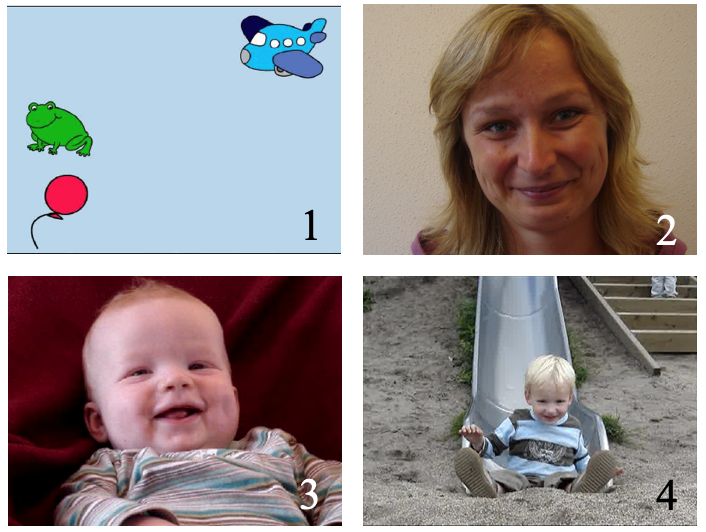
\includegraphics[width=0.7\linewidth]{figures/chapter_4/Figure1} 

}

\caption{Visual stimuli presented during the pre- and posttest, habituation and test phase. Picture 1 is an example of the visual stimuli during pre-and posttest; 2 is an example of a female face used during habitation and test trials; 3 is a still of the attention getter between habituation trials and 4 is a still of the attention getter between test trials.}\label{fig:ch04fig1}
\end{figure}

\hypertarget{procedure}{%
\subsection{Procedure}\label{procedure}}

Infants were seated on their caretaker's lap in a sound-attenuated booth. As soon as infants looked towards the computer screen in front of them, the experimenter started the first trial. In each trial, the time the participant was looking at the screen was measured. Whenever the participant looked away for 2 consecutive seconds, the trial was ended; a new one started when the infant oriented to the screen again. There was no minimum looking time to the screen. Looking times were coded online using a button box connected to the computer controlling the experiment and acquiring data.

Pre- and posttest were used to gauge participants' general attentiveness. If total looking time to the posttest stimulus was less than 50\% of the total looking time to the pretest stimulus, the participant was considered to be showing a general loss of attention and was discarded for analysis. This was never the case in our sample (see Participants).

The habituation phase consisted of a maximum of 12 trials, with a maximum of 30 repetitions of a token per trial (ISI of 1 second) resulting in a total duration of approximately 48 seconds. A 65\% habituation criterion was used to determine whether the participant had habituated. To determine whether the habituation criterion was met, a moving window was used (Figure \ref{fig:ch04fig2}). The mean looking times of the first three trials (1-3) was compared to the subsequent three trials (4-6): if looking time had decreased by (minimally) 35\%, the criterion was met. If not, the mean looking time of trial 1-3 was compared to 5-7, 6-8, etc., and the same criterion applied, up until the final subset 10-12. Infants who did not meet the habituation criterion were not included in data analysis (\(n = 5\), see Participants). The selection of habituation stimuli (faap (/fa:p/) or feep (/fe:p/)) was counterbalanced between
infants. Infants were presented with all four voices, in randomized order: in each block of four trials the infant heard all four voices but in randomized order within the blocks (see Figure \ref{fig:ch04fig3}).

The test phase included a fixed number of 12 trials, with a maximum number of 30 tokens per trial, resulting in a duration of approximately 48 seconds per trial. Houston et al. (\protect\hyperlink{ref-houston_assessing_2007}{2007}) used 14 test trials (10 non-alternating and 4 alternating). We reduced the number of test phase trials and thus duration, because we know from experience that Dutch infants are not always able to sit through experiments that have the same duration as those conducted with infants in the US. Of these 12 test trials, four were alternating (e.g.~/fe:p/-/fa:p/), and 8 non-alternating (e.g.~/fa:p/-/fa:p/). The alternating and non-alternating trials were presented in a semi-fixed order: the first trial could be either alternating or non-alternating, which was counterbalanced. Three subsequent alternating trials occurred at positions: 5, 8 and 12. During the test phase a new token of one familiar speaker was introduced, either nonalternating
or alternating (see Figure \ref{fig:ch04fig3}.

\begin{figure}

{\centering 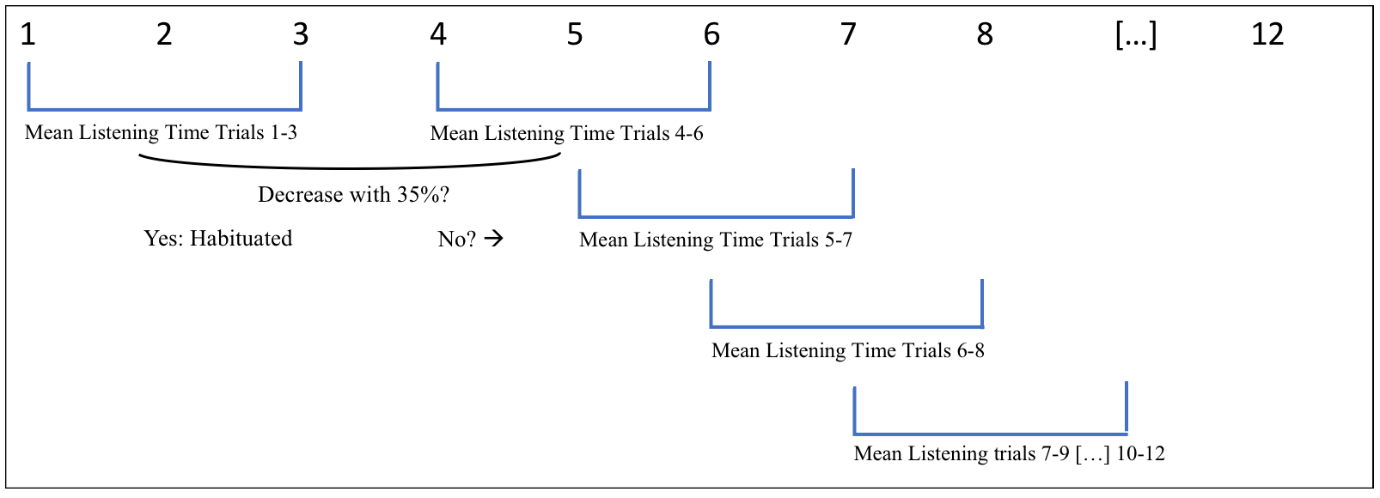
\includegraphics[width=0.9\linewidth]{figures/chapter_4/Figure2} 

}

\caption{Visual depiction of the assessment of the (65\%) habituation criterion}\label{fig:ch04fig2}
\end{figure}

\begin{figure}

{\centering 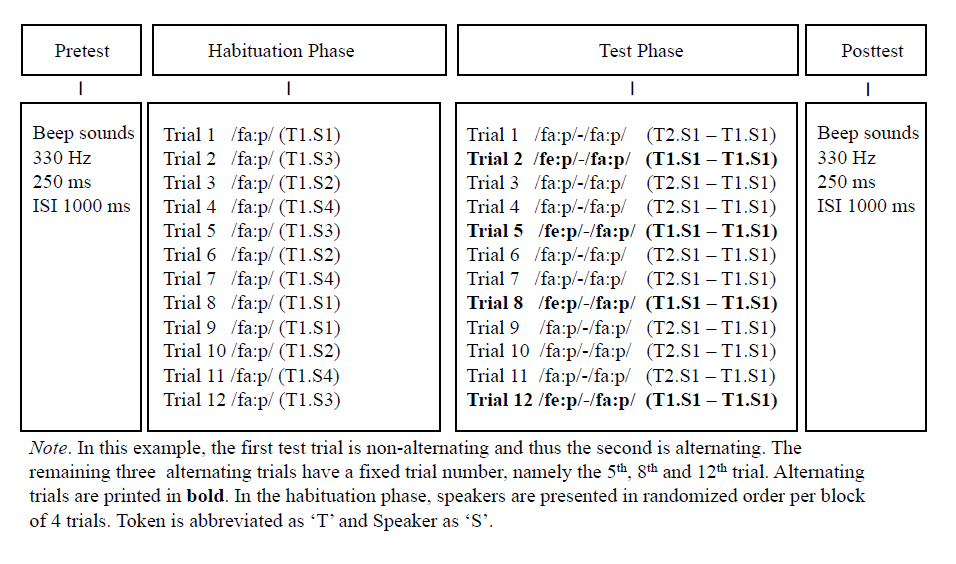
\includegraphics[width=0.9\linewidth]{figures/chapter_4/Figure3} 

}

\caption{Schematic overview of the experimental procedure with reference to the auditory stimuli only. In this example, the first test trial is non-alternating and consequently the second is alternating. The remaining three alternating trials have a fixed number, viz. the 5th, the 8th and 12th trial. Alternating trials are printed in bold. Token is abbreviated as 'T' and Speakers as 'S'}\label{fig:ch04fig3}
\end{figure}

\hypertarget{results-3}{%
\section{Results}\label{results-3}}

\hypertarget{summary-of-the-group-data-published-in-de_klerk_lost_2019}{%
\subsection{\texorpdfstring{Summary of the group data published in Klerk et al. (\protect\hyperlink{ref-de_klerk_lost_2019}{2019})}{Summary of the group data published in Klerk et al. (2019)}}\label{summary-of-the-group-data-published-in-de_klerk_lost_2019}}

The group-based data is presented in Figure \ref{fig:ch04fig4} and Table \ref{tab:ch04tab2}. Mixed Modeling using SPSS (version 23) with Subjects as random factor, Trial Number as a repeated effect (covariance structure AR1), and Trial type (alternating vs.~non-alternating) and Age as the fixed factors showed that at group level, infants between 6-10 months of age discriminated /fa:p/ from /fe:p/, at group level (Klerk et al., \protect\hyperlink{ref-de_klerk_lost_2019}{2019}). In the current study we focus on the individual data.

\begin{figure}

{\centering 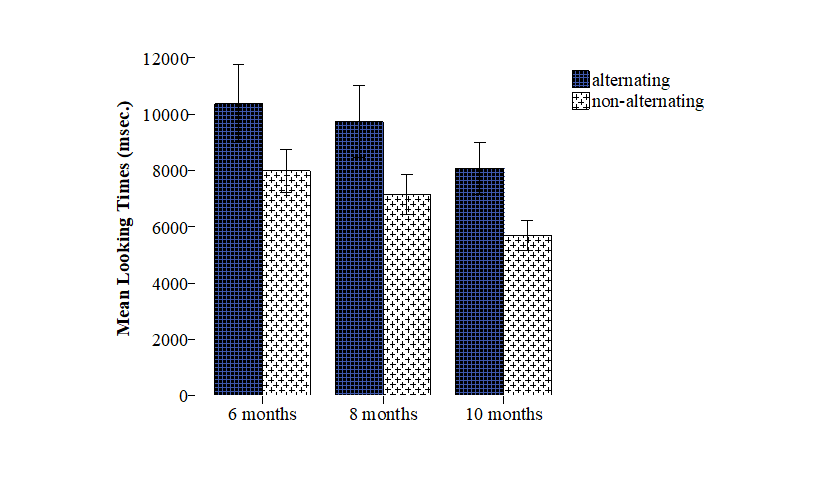
\includegraphics[width=0.9\linewidth]{figures/chapter_4/Figure4} 

}

\caption{Raw mean looking times (milliseconds) to alternating and non-alternating trials per age group. Error bars represent Confidence Intervals (95\%).}\label{fig:ch04fig4}
\end{figure}

\begin{longtable}[]{@{}cclccll@{}}
\caption{\label{tab:ch04tab2} Listening Times (seconds) to Alternating and Non-Alternating Trials}\tabularnewline
\toprule
\begin{minipage}[b]{0.09\columnwidth}\centering
Age Group\strut
\end{minipage} & \begin{minipage}[b]{0.15\columnwidth}\centering
Infants\strut
\end{minipage} & \begin{minipage}[b]{0.15\columnwidth}\raggedright
Alternating trials\strut
\end{minipage} & \begin{minipage}[b]{0.12\columnwidth}\centering
Non-alternating
Trials\strut
\end{minipage} & \begin{minipage}[b]{0.09\columnwidth}\centering
Statistics\strut
\end{minipage} & \begin{minipage}[b]{0.09\columnwidth}\raggedright
\strut
\end{minipage} & \begin{minipage}[b]{0.11\columnwidth}\raggedright
\strut
\end{minipage}\tabularnewline
\midrule
\endfirsthead
\toprule
\begin{minipage}[b]{0.09\columnwidth}\centering
Age Group\strut
\end{minipage} & \begin{minipage}[b]{0.15\columnwidth}\centering
Infants\strut
\end{minipage} & \begin{minipage}[b]{0.15\columnwidth}\raggedright
Alternating trials\strut
\end{minipage} & \begin{minipage}[b]{0.12\columnwidth}\centering
Non-alternating
Trials\strut
\end{minipage} & \begin{minipage}[b]{0.09\columnwidth}\centering
Statistics\strut
\end{minipage} & \begin{minipage}[b]{0.09\columnwidth}\raggedright
\strut
\end{minipage} & \begin{minipage}[b]{0.11\columnwidth}\raggedright
\strut
\end{minipage}\tabularnewline
\midrule
\endhead
\begin{minipage}[t]{0.09\columnwidth}\centering
\strut
\end{minipage} & \begin{minipage}[t]{0.15\columnwidth}\centering
\(N\)\strut
\end{minipage} & \begin{minipage}[t]{0.15\columnwidth}\raggedright
\emph{M (SD)}\strut
\end{minipage} & \begin{minipage}[t]{0.12\columnwidth}\centering
\emph{M (SD)}\strut
\end{minipage} & \begin{minipage}[t]{0.09\columnwidth}\centering
F\strut
\end{minipage} & \begin{minipage}[t]{0.09\columnwidth}\raggedright
\emph{p}\strut
\end{minipage} & \begin{minipage}[t]{0.11\columnwidth}\raggedright
\emph{Cohen's d}\strut
\end{minipage}\tabularnewline
\begin{minipage}[t]{0.09\columnwidth}\centering
6\strut
\end{minipage} & \begin{minipage}[t]{0.15\columnwidth}\centering
38\strut
\end{minipage} & \begin{minipage}[t]{0.15\columnwidth}\raggedright
10.4 (8.6)\strut
\end{minipage} & \begin{minipage}[t]{0.12\columnwidth}\centering
7.9 (6.8)\strut
\end{minipage} & \begin{minipage}[t]{0.09\columnwidth}\centering
13.55\strut
\end{minipage} & \begin{minipage}[t]{0.09\columnwidth}\raggedright
\textless{} .001\strut
\end{minipage} & \begin{minipage}[t]{0.11\columnwidth}\raggedright
.31\strut
\end{minipage}\tabularnewline
\begin{minipage}[t]{0.09\columnwidth}\centering
8\strut
\end{minipage} & \begin{minipage}[t]{0.15\columnwidth}\centering
44\strut
\end{minipage} & \begin{minipage}[t]{0.15\columnwidth}\raggedright
9.7 (8.6)\strut
\end{minipage} & \begin{minipage}[t]{0.12\columnwidth}\centering
7.1 (6.7)\strut
\end{minipage} & \begin{minipage}[t]{0.09\columnwidth}\centering
21.74\strut
\end{minipage} & \begin{minipage}[t]{0.09\columnwidth}\raggedright
\textless{} .001\strut
\end{minipage} & \begin{minipage}[t]{0.11\columnwidth}\raggedright
.32\strut
\end{minipage}\tabularnewline
\begin{minipage}[t]{0.09\columnwidth}\centering
10\strut
\end{minipage} & \begin{minipage}[t]{0.15\columnwidth}\centering
35\strut
\end{minipage} & \begin{minipage}[t]{0.15\columnwidth}\raggedright
8.1 (5.6)\strut
\end{minipage} & \begin{minipage}[t]{0.12\columnwidth}\centering
5.7 (4.5)\strut
\end{minipage} & \begin{minipage}[t]{0.09\columnwidth}\centering
29.24\strut
\end{minipage} & \begin{minipage}[t]{0.09\columnwidth}\raggedright
\textless{} .001\strut
\end{minipage} & \begin{minipage}[t]{0.11\columnwidth}\raggedright
.45\strut
\end{minipage}\tabularnewline
\begin{minipage}[t]{0.09\columnwidth}\centering
\textbf{All}\strut
\end{minipage} & \begin{minipage}[t]{0.15\columnwidth}\centering
\textbf{117}\strut
\end{minipage} & \begin{minipage}[t]{0.15\columnwidth}\raggedright
\textbf{9.4 (7.9)}\strut
\end{minipage} & \begin{minipage}[t]{0.12\columnwidth}\centering
\textbf{7.0 (6.3)}\strut
\end{minipage} & \begin{minipage}[t]{0.09\columnwidth}\centering
\textbf{62.70}\strut
\end{minipage} & \begin{minipage}[t]{0.09\columnwidth}\raggedright
\textbf{\textless{} .001}\strut
\end{minipage} & \begin{minipage}[t]{0.11\columnwidth}\raggedright
\textbf{.32}\strut
\end{minipage}\tabularnewline
\bottomrule
\end{longtable}

\newpage

\hypertarget{data-screening}{%
\subsection{Data Screening}\label{data-screening}}

The raw looking times to alternating and non-alternating trials were not normally distributed; for this reason, a log transformation (Log10) was performed. After this transformation the skewness (.123, SE = .065) and kurtosis (.150, SE = .131) values were acceptable. We refer to the supplementary files for histograms of the raw and log transformed data \href{https://osf.io/ebrxy/}{(https://osf.io/ebrxy/)}.

\hypertarget{analysis-1-linear-regression-model-with-autoregressive-ar1-error-structure}{%
\subsection{Analysis 1: Linear Regression Model with Autoregressive (AR1) Error Structure}\label{analysis-1-linear-regression-model-with-autoregressive-ar1-error-structure}}

To assess individual performance, we used the same regression model with autoregressive effect as Houston et al. (\protect\hyperlink{ref-houston_assessing_2007}{2007}),

\begin{equation}
\begin{array}{l}
    y_t = b_0 + b_1 C_t + a_t \\ 
    a_t =
\begin{cases}
    \phi_1 a_{t-1} + e_t,& \text{if } t\geq 1\\
    0,              & \text{otherwise}
\end{cases}
\end{array}
\end{equation}

where subscript \(t\) denotes the trial number \(t=1,...,T\), \(y\), denotes the looking time of the trial, \(C\) denotes the condition (alternating or non-alternating) of the trial, \(e\) denotes the error term, \(\phi_1\) denotes the autoregressive factor. In this model \(b_1C_t\) accounts for the influence of the condition and \(b_1\) is interpreted as the difference in looking time for the two conditions. the dependence on the looking time of the previous trial is found in the specification of the error structure \(\phi_1a_{t-1}\). The error in the current time point (\(a_t\)) is dependent on the error of the previous time point (\(a_{t-1}\)), except for \(a_1\), because \(a_1\) is the first trial. There is no carry-over effect from the previous trial and no autoregressive effect. Looking times and statistical outcomes per infant are reported in Appendix \protect\hyperlink{ch05appendix}{A}. Individual analyses show that condition effects were significant for 14 participants, implying that only 12\% of the infants were able to discriminate between alternating and non-alternating trials. When we correct for multiple testing using the Benjamini-Hochberg procedure (Benjamini \& Hochberg, \protect\hyperlink{ref-benjamini_controlling_1995}{1995}), this number decreases to 3 infants (3/117), a mere 3\%.

Our results do not align with the results of the study of Houston et al. (\protect\hyperlink{ref-houston_assessing_2007}{2007}), in which 80\% (8/10) of the 9-month-old infants successfully discriminated the contrast. Applying the Benjamini-Hochberg correction for multiple testing to Houston et al. (\protect\hyperlink{ref-houston_assessing_2007}{2007}) data did not make a difference in their outcomes, because of the few participants tested and the large effect of condition on looking times. Nevertheless, an analysis without having to correct for multiple testing is desirable and Bayesian modeling could be a solution.

\hypertarget{analysis-2-hierarchical-bayesian-analysis}{%
\subsection{Analysis 2: Hierarchical Bayesian Analysis}\label{analysis-2-hierarchical-bayesian-analysis}}

The analyses used in the paper by Houston et al. (\protect\hyperlink{ref-houston_assessing_2007}{2007}) rely on separate regression analyses for each individual child. However, if we assume that infants are exchangeable within the same age group, that is, that they come from the same population, an alternative and more powerful approach is to model their looking times in a hierarchical (multilevel) structure. By modeling both the individual and group effects in one analysis instead of doing so for 117 separate analyses, one for each individual, part of the observed variance could be explained at the group level instead of trying to explain all variance at the individual level. As a result, we will have reduced uncertainty in our estimates for the individual parameters (Gelman, \protect\hyperlink{ref-gelman_multilevel_2006}{2006}\protect\hyperlink{ref-gelman_multilevel_2006}{a}). Moreover, by using a Bayesian hierarchical analysis, we are able to obtain estimates for each of the individual and group parameters in one model without the need to correct for multiple testing (Gelman et al., \protect\hyperlink{ref-gelman_why_2012}{2012}).

In our Bayesian hierarchical regression, we modelled the individual infant data in three groups based on their age (6, 8 and 10 months). We used the same model as before, namely a regression model with an AR1 error structure, with Log10 transformed looking times as outcomes and condition (alternating or non-alternating trial) as predictor. For all groups we obtained both group and individual estimates for the intercept (looking time alternating trials), the condition (difference in looking time between alternating and non-alternating trials) and the AR1 effect. Details on the priors, estimation, model fit and sensitivity analyses are given in the supplementary files on the Open Science Framework webpage for this study at (\url{https://osf.io/ebrxy/}) or in Appendix \protect\hyperlink{ch05appendixB}{B}. In short, we achieve a good model fit.

The parameter of interest was the condition parameter. This parameter allowed us to establish whether the looking times differed between the alternating and non-alternating condition for the individual infants. To keep the decision criterion as similar as possible to the previously described analyses, we checked how many of the infants included the value 0 in their 95\% credibility interval (CI) for the condition parameter. For the 95\% CI (the 0.025 and 0.975 quantiles of the posterior sample) we regard this interval as having a 95\% probability of containing the unknown parameter value. In contrast, the 95\% Confidence Interval in frequentist statistics relates to (potential) replications of the experiment and expresses the expectation that the interval contains the true parameter estimate in 95\% of the experiments. In our study, the percentages of infants whose 95\% CI did not include 0 are displayed per age group in Table \ref{tab:ch04tab3}. For the 10-months-olds we found that 77\% discriminated between the alternating and non-alternating condition, and 53\% of the 6-month-olds did, whilst for the 8-month-old infants this was only 27\%.

\begin{longtable}[]{@{}llclc@{}}
\caption{\label{tab:ch04tab3} Number and Percentage of Infants that Discriminate the Contrast Significantly per Age Group and of Infants that did not include the Value 0 in Their 95\% Credibility Interval (CI)}\tabularnewline
\toprule
\begin{minipage}[b]{0.09\columnwidth}\raggedright
\strut
\end{minipage} & \begin{minipage}[b]{0.15\columnwidth}\raggedright
\strut
\end{minipage} & \begin{minipage}[b]{0.16\columnwidth}\centering
Frequentist
(non-hierarchical)
modeling\strut
\end{minipage} & \begin{minipage}[b]{0.16\columnwidth}\raggedright
\strut
\end{minipage} & \begin{minipage}[b]{0.28\columnwidth}\centering
Bayesian Hierarchical modeling\strut
\end{minipage}\tabularnewline
\midrule
\endfirsthead
\toprule
\begin{minipage}[b]{0.09\columnwidth}\raggedright
\strut
\end{minipage} & \begin{minipage}[b]{0.15\columnwidth}\raggedright
\strut
\end{minipage} & \begin{minipage}[b]{0.16\columnwidth}\centering
Frequentist
(non-hierarchical)
modeling\strut
\end{minipage} & \begin{minipage}[b]{0.16\columnwidth}\raggedright
\strut
\end{minipage} & \begin{minipage}[b]{0.28\columnwidth}\centering
Bayesian Hierarchical modeling\strut
\end{minipage}\tabularnewline
\midrule
\endhead
\begin{minipage}[t]{0.09\columnwidth}\raggedright
Age Group\strut
\end{minipage} & \begin{minipage}[t]{0.15\columnwidth}\raggedright
Participants\strut
\end{minipage} & \begin{minipage}[t]{0.16\columnwidth}\centering
Uncorrected
Successful
Discrimination (\%)\strut
\end{minipage} & \begin{minipage}[t]{0.16\columnwidth}\raggedright
Corrected
Successful
Discrimination (\%)\strut
\end{minipage} & \begin{minipage}[t]{0.28\columnwidth}\centering
Infants without 0 in their 95\% CI
(\%)\strut
\end{minipage}\tabularnewline
\begin{minipage}[t]{0.09\columnwidth}\raggedright
6\strut
\end{minipage} & \begin{minipage}[t]{0.15\columnwidth}\raggedright
38\strut
\end{minipage} & \begin{minipage}[t]{0.16\columnwidth}\centering
2 (5)\strut
\end{minipage} & \begin{minipage}[t]{0.16\columnwidth}\raggedright
0 (0)\strut
\end{minipage} & \begin{minipage}[t]{0.28\columnwidth}\centering
20 (53)\strut
\end{minipage}\tabularnewline
\begin{minipage}[t]{0.09\columnwidth}\raggedright
8\strut
\end{minipage} & \begin{minipage}[t]{0.15\columnwidth}\raggedright
44\strut
\end{minipage} & \begin{minipage}[t]{0.16\columnwidth}\centering
4 (9)\strut
\end{minipage} & \begin{minipage}[t]{0.16\columnwidth}\raggedright
2 (5)\strut
\end{minipage} & \begin{minipage}[t]{0.28\columnwidth}\centering
12 (27)\strut
\end{minipage}\tabularnewline
\begin{minipage}[t]{0.09\columnwidth}\raggedright
10\strut
\end{minipage} & \begin{minipage}[t]{0.15\columnwidth}\raggedright
35\strut
\end{minipage} & \begin{minipage}[t]{0.16\columnwidth}\centering
8 (23)\strut
\end{minipage} & \begin{minipage}[t]{0.16\columnwidth}\raggedright
1 (3)\strut
\end{minipage} & \begin{minipage}[t]{0.28\columnwidth}\centering
27 (77)\strut
\end{minipage}\tabularnewline
\begin{minipage}[t]{0.09\columnwidth}\raggedright
\textbf{Ttoal}\strut
\end{minipage} & \begin{minipage}[t]{0.15\columnwidth}\raggedright
\textbf{117}\strut
\end{minipage} & \begin{minipage}[t]{0.16\columnwidth}\centering
\textbf{14 (12)}\strut
\end{minipage} & \begin{minipage}[t]{0.16\columnwidth}\raggedright
\textbf{3 (3)}\strut
\end{minipage} & \begin{minipage}[t]{0.28\columnwidth}\centering
\textbf{59 (50)}\strut
\end{minipage}\tabularnewline
\bottomrule
\end{longtable}

\newpage

\begin{figure}

{\centering 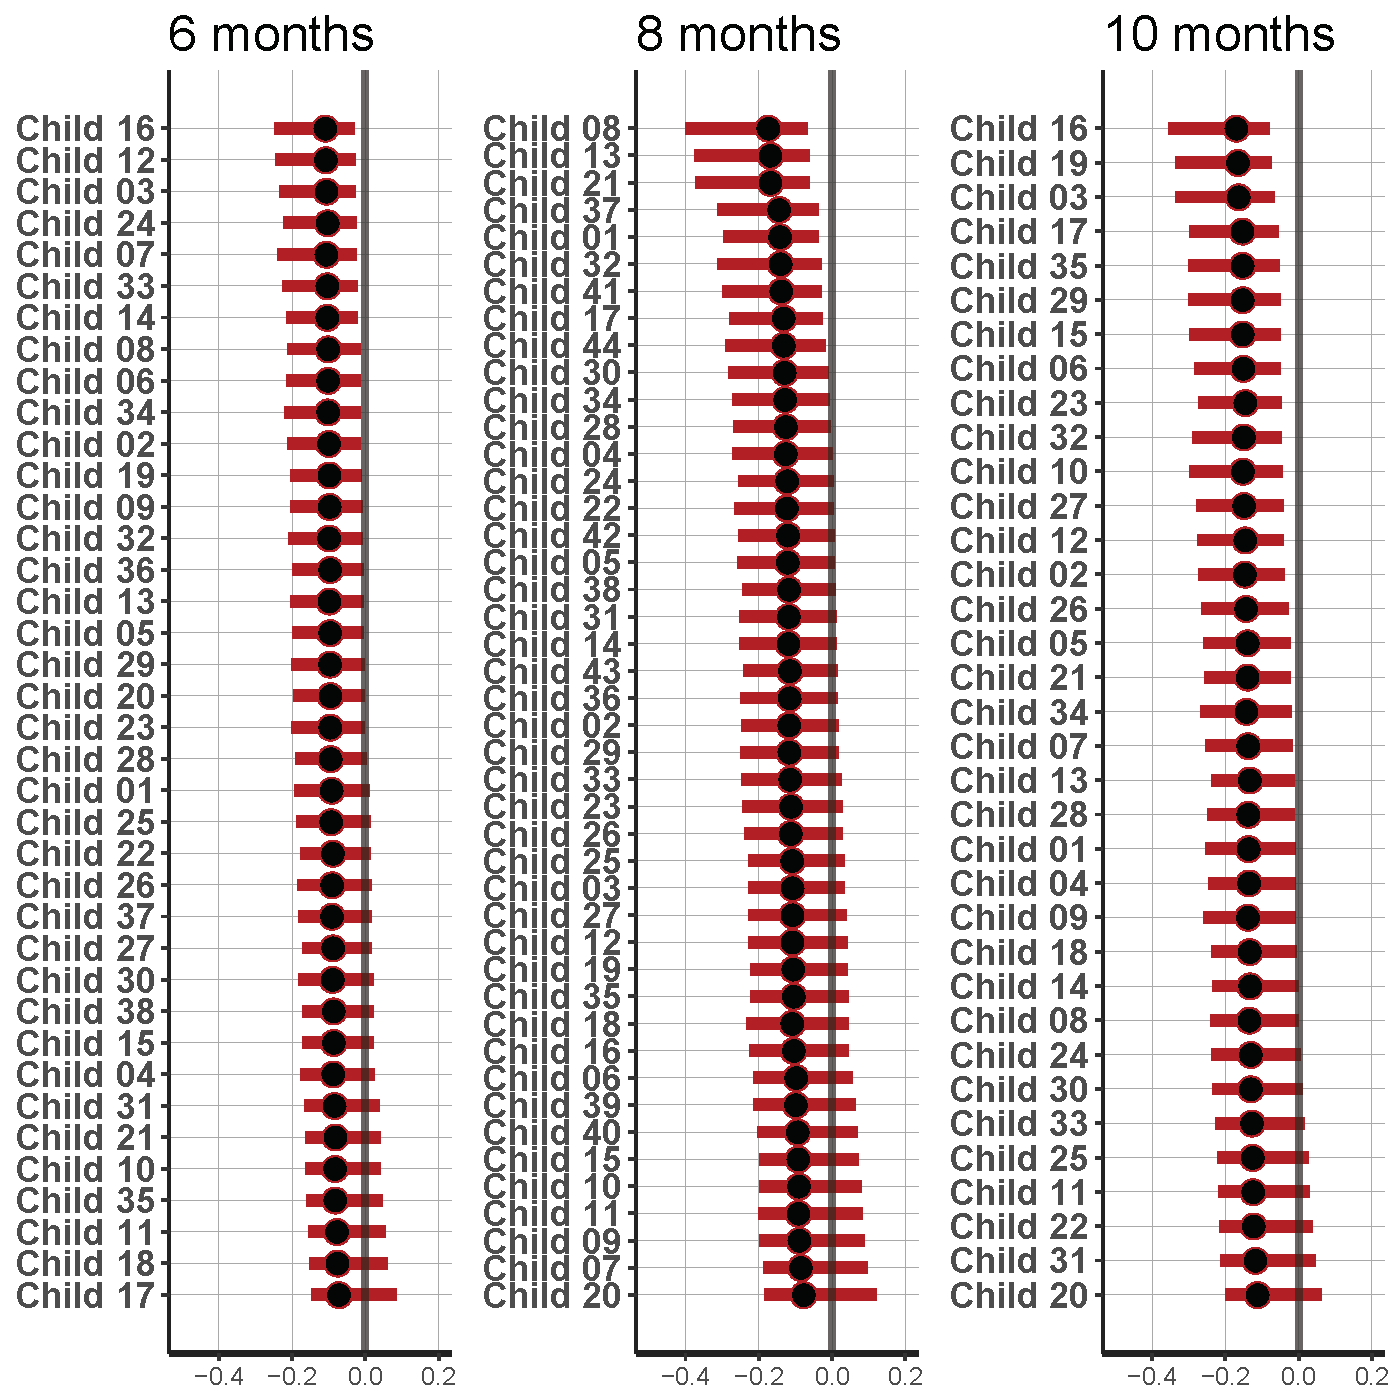
\includegraphics[width=0.9\linewidth]{figures/chapter_4/Figure5} 

}

\caption{Results of the hierarchical model for each individual per age group. The black dots represent the median; the red bars represent the 95\% Credibility Intervals.}\label{fig:ch04fig5}
\end{figure}

Figure \ref{fig:ch04fig5} shows the results of the hierarchical model for each individual per age group. Credibility Intervals for the 8-month-old infants show larger uncertainty for the estimates than for the other two age groups, especially the 6-month-olds. The group-estimated effect of condition, depicted in the left panel of Figure \ref{fig:ch04fig6}, increases with age. The estimated random effect for condition is largest in the 8-month-old group, which can be seen from the variance estimates in the right panel of Figure \ref{fig:ch04fig6}. Because the infants of the 8-month-old group differ more from one another than the infants in the other age groups, less shrinkage of estimates occurs and we remain more uncertain about their estimated condition effects. This outcome is visible in the larger credibility intervals for the infants in age group 8 compared to the other two age groups.

\begin{figure}

{\centering 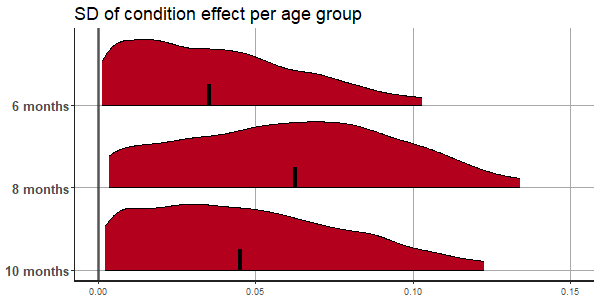
\includegraphics[width=0.9\linewidth]{figures/chapter_4/Figure6} 

}

\caption{Group estimates for condition effects and variation per age group.  The left panel shows the group estimates for condition effects. The right panel shows the standard deviation of the condition effect per age group. The densities, presented in red, represent the 95\% credibility interval.}\label{fig:ch04fig6}
\end{figure}

As part of the model assessment we conducted posterior predictive checks. These checks provide insight into the plausibility to the hypothesized and estimated model by drawing simulations from the posterior model. Figure \ref{fig:ch04fig7} shows how well the model fits the data of a particular child, in this case child 16 in age group 6. Simulations are based on the posterior parameter estimates for this specific child at each specific measurement, taking into account the child-specific estimated looking times for (non-)alternating trials, the child-specific condition effect and the child-specific autoregressive effect. The posterior predictive \(p\)-value (ppp) indicates the proportion of simulated values for this measurement that are smaller than the observed value. If `ppp' falls between 0.025 and 0.975 we conclude that our model provides an accurate prediction for this specific observation. Note that this specific child 16 is classified as non-discriminator and that all measurements are accurately captured by the model as shown by the blue bars in each histogram (Figure \ref{fig:ch04fig7}). For an example of a child classified as non-discriminator with less accurate model descriptions for the observed measurement see for instance child 17 from age group 10, measurements (trials) 5 and 7 (see \url{https://osf.io/ebrxy/}).

\begin{figure}

{\centering 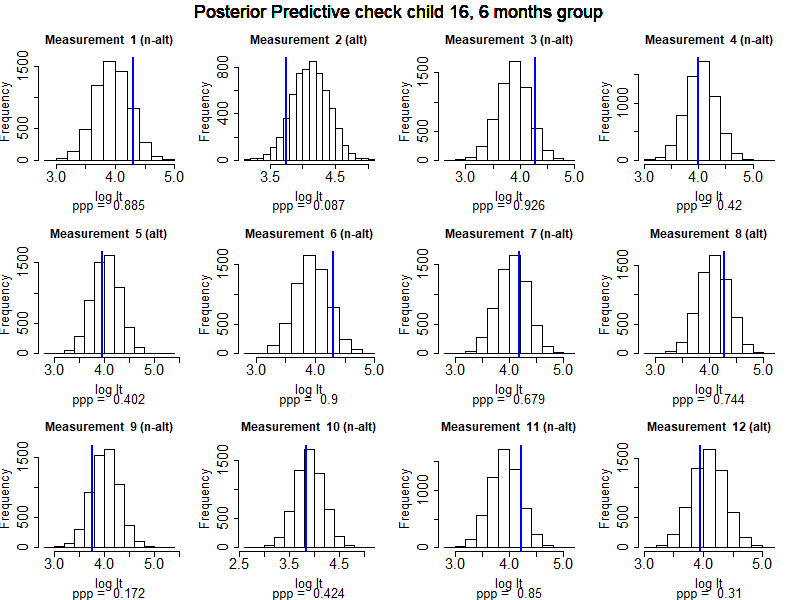
\includegraphics[width=0.9\linewidth]{figures/chapter_4/Figure7} 

}

\caption{Posterior predictive simulations for child 16 in age group 6 for all 12 observed trials. Each histogram contains 6000 simulated values for that particular observation of that specific child based on the posterior parameter estimates. The blue vertical line denotes the actually observed value for the specific measurement.}\label{fig:ch04fig7}
\end{figure}

To evaluate the effects of the hierarchical regression compared to modelling the individual regressions, we also ran Bayesian regression analyses with AR1 error structure without the multilevel structure. Figure \ref{fig:ch04fig8} shows the estimates with their uncertainty for the condition parameter for all infants in age group 6 (only); the other groups show similar patterns. The figure shows that including the hierarchical structure reduced the uncertainty of the estimates markedly.

\begin{figure}

{\centering 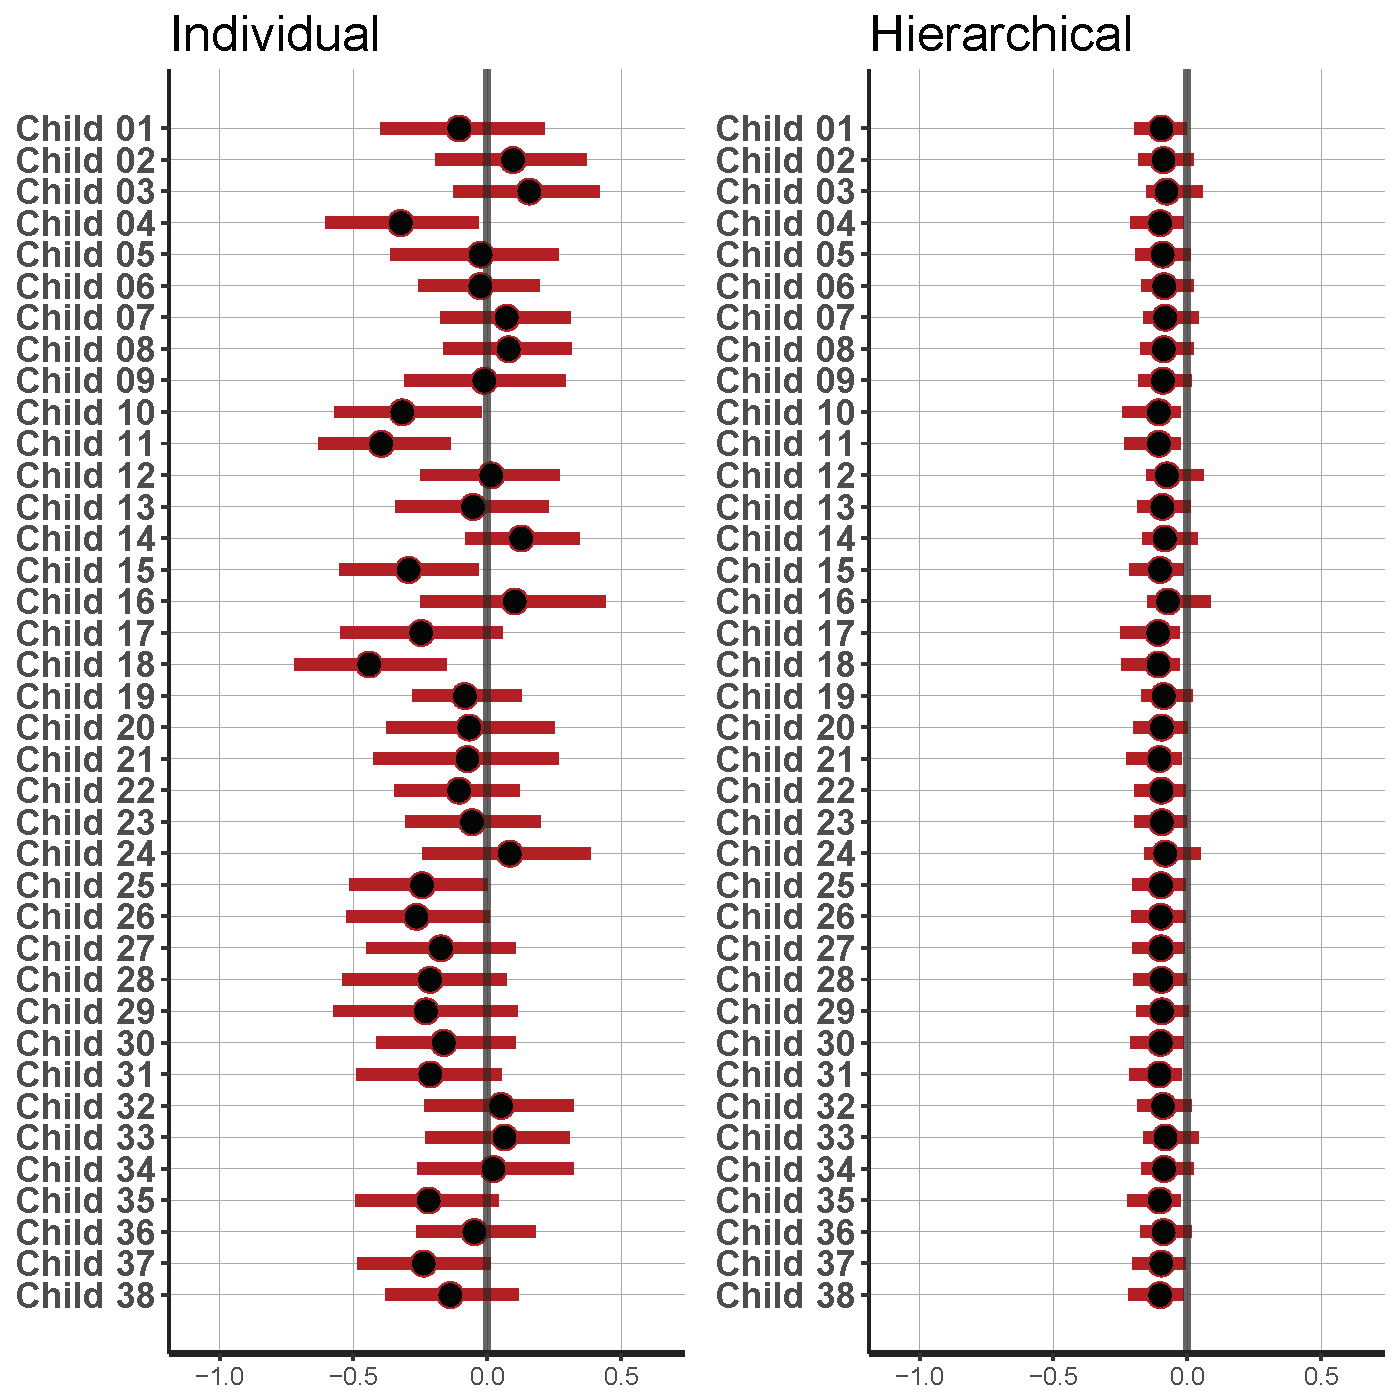
\includegraphics[width=0.9\linewidth]{figures/chapter_4/Figure8} 

}

\caption{Comparison of results of individual and hierarchical analyses for condition parameter of each infant in the 6-month-olds group. The Hierarchical model reduces the uncertainty (95\% CI represented by red bar) (median represented by the black dot) for the parameter estimates.}\label{fig:ch04fig8}
\end{figure}

Table \ref{tab:ch04tab4} displays the mean log-transformed looking time differences between the alternating and non-alternating trials for all individuals that did not include the value 0 in their 95\% CI for the condition effect in the hierarchical regression. These raw data show the direction of the average difference in looking time between alternating and non-alternating trials, as well as the magnitude of the average difference between trial types. As can be seen, both looking time difference directions are present, meaning that the data set includes infants with on average longer looks to alternating trials as well as infants with on average longer looks to non-alternating trials. In addition, Table \ref{tab:ch04tab4} shows that the magnitude of looking time differences between alternating and non-alternating trials shows considerable variation.

\begin{longtable}[]{@{}cccccc@{}}
\caption{\label{tab:ch04tab4} The Mean Looking Time Difference between Alternating and Non-Alternating Trials for the Infants whose Confidence Interval (95\%) did not cross the Value 0. The mean log-transformed looking time differences are presented.}\tabularnewline
\toprule
\begin{minipage}[b]{0.11\columnwidth}\centering
Subject\strut
\end{minipage} & \begin{minipage}[b]{0.09\columnwidth}\centering
Group\strut
\end{minipage} & \begin{minipage}[b]{0.18\columnwidth}\centering
Difference\strut
\end{minipage} & \begin{minipage}[b]{0.11\columnwidth}\centering
Subject\strut
\end{minipage} & \begin{minipage}[b]{0.11\columnwidth}\centering
Group\strut
\end{minipage} & \begin{minipage}[b]{0.21\columnwidth}\centering
Difference\strut
\end{minipage}\tabularnewline
\midrule
\endfirsthead
\toprule
\begin{minipage}[b]{0.11\columnwidth}\centering
Subject\strut
\end{minipage} & \begin{minipage}[b]{0.09\columnwidth}\centering
Group\strut
\end{minipage} & \begin{minipage}[b]{0.18\columnwidth}\centering
Difference\strut
\end{minipage} & \begin{minipage}[b]{0.11\columnwidth}\centering
Subject\strut
\end{minipage} & \begin{minipage}[b]{0.11\columnwidth}\centering
Group\strut
\end{minipage} & \begin{minipage}[b]{0.21\columnwidth}\centering
Difference\strut
\end{minipage}\tabularnewline
\midrule
\endhead
\begin{minipage}[t]{0.11\columnwidth}\centering
\strut
\end{minipage} & \begin{minipage}[t]{0.09\columnwidth}\centering
\emph{Age}\strut
\end{minipage} & \begin{minipage}[t]{0.18\columnwidth}\centering
\emph{alternating} -
\emph{nonalternating}\strut
\end{minipage} & \begin{minipage}[t]{0.11\columnwidth}\centering
\strut
\end{minipage} & \begin{minipage}[t]{0.11\columnwidth}\centering
\emph{Age}\strut
\end{minipage} & \begin{minipage}[t]{0.21\columnwidth}\centering
\emph{alternating} -
\emph{nonalternating}\strut
\end{minipage}\tabularnewline
\begin{minipage}[t]{0.11\columnwidth}\centering
child 02\strut
\end{minipage} & \begin{minipage}[t]{0.09\columnwidth}\centering
6\strut
\end{minipage} & \begin{minipage}[t]{0.18\columnwidth}\centering
-.10\strut
\end{minipage} & \begin{minipage}[t]{0.11\columnwidth}\centering
child 41\strut
\end{minipage} & \begin{minipage}[t]{0.11\columnwidth}\centering
8\strut
\end{minipage} & \begin{minipage}[t]{0.21\columnwidth}\centering
-.27\strut
\end{minipage}\tabularnewline
\begin{minipage}[t]{0.11\columnwidth}\centering
child 03\strut
\end{minipage} & \begin{minipage}[t]{0.09\columnwidth}\centering
6\strut
\end{minipage} & \begin{minipage}[t]{0.18\columnwidth}\centering
-.14\strut
\end{minipage} & \begin{minipage}[t]{0.11\columnwidth}\centering
child 44\strut
\end{minipage} & \begin{minipage}[t]{0.11\columnwidth}\centering
8\strut
\end{minipage} & \begin{minipage}[t]{0.21\columnwidth}\centering
-.07\strut
\end{minipage}\tabularnewline
\begin{minipage}[t]{0.11\columnwidth}\centering
child 05\strut
\end{minipage} & \begin{minipage}[t]{0.09\columnwidth}\centering
6\strut
\end{minipage} & \begin{minipage}[t]{0.18\columnwidth}\centering
-.03\strut
\end{minipage} & \begin{minipage}[t]{0.11\columnwidth}\centering
child 01\strut
\end{minipage} & \begin{minipage}[t]{0.11\columnwidth}\centering
10\strut
\end{minipage} & \begin{minipage}[t]{0.21\columnwidth}\centering
.12\strut
\end{minipage}\tabularnewline
\begin{minipage}[t]{0.11\columnwidth}\centering
child 06\strut
\end{minipage} & \begin{minipage}[t]{0.09\columnwidth}\centering
6\strut
\end{minipage} & \begin{minipage}[t]{0.18\columnwidth}\centering
.03\strut
\end{minipage} & \begin{minipage}[t]{0.11\columnwidth}\centering
child 02\strut
\end{minipage} & \begin{minipage}[t]{0.11\columnwidth}\centering
10\strut
\end{minipage} & \begin{minipage}[t]{0.21\columnwidth}\centering
.13\strut
\end{minipage}\tabularnewline
\begin{minipage}[t]{0.11\columnwidth}\centering
child 07\strut
\end{minipage} & \begin{minipage}[t]{0.09\columnwidth}\centering
6\strut
\end{minipage} & \begin{minipage}[t]{0.18\columnwidth}\centering
-.10\strut
\end{minipage} & \begin{minipage}[t]{0.11\columnwidth}\centering
child 03\strut
\end{minipage} & \begin{minipage}[t]{0.11\columnwidth}\centering
10\strut
\end{minipage} & \begin{minipage}[t]{0.21\columnwidth}\centering
-.09\strut
\end{minipage}\tabularnewline
\begin{minipage}[t]{0.11\columnwidth}\centering
child 08\strut
\end{minipage} & \begin{minipage}[t]{0.09\columnwidth}\centering
6\strut
\end{minipage} & \begin{minipage}[t]{0.18\columnwidth}\centering
-.01\strut
\end{minipage} & \begin{minipage}[t]{0.11\columnwidth}\centering
child 04\strut
\end{minipage} & \begin{minipage}[t]{0.11\columnwidth}\centering
10\strut
\end{minipage} & \begin{minipage}[t]{0.21\columnwidth}\centering
.25\strut
\end{minipage}\tabularnewline
\begin{minipage}[t]{0.11\columnwidth}\centering
child 09\strut
\end{minipage} & \begin{minipage}[t]{0.09\columnwidth}\centering
6\strut
\end{minipage} & \begin{minipage}[t]{0.18\columnwidth}\centering
-.02\strut
\end{minipage} & \begin{minipage}[t]{0.11\columnwidth}\centering
child 05\strut
\end{minipage} & \begin{minipage}[t]{0.11\columnwidth}\centering
10\strut
\end{minipage} & \begin{minipage}[t]{0.21\columnwidth}\centering
.11\strut
\end{minipage}\tabularnewline
\begin{minipage}[t]{0.11\columnwidth}\centering
child 12\strut
\end{minipage} & \begin{minipage}[t]{0.09\columnwidth}\centering
6\strut
\end{minipage} & \begin{minipage}[t]{0.18\columnwidth}\centering
-.05\strut
\end{minipage} & \begin{minipage}[t]{0.11\columnwidth}\centering
child 06\strut
\end{minipage} & \begin{minipage}[t]{0.11\columnwidth}\centering
10\strut
\end{minipage} & \begin{minipage}[t]{0.21\columnwidth}\centering
.09\strut
\end{minipage}\tabularnewline
\begin{minipage}[t]{0.11\columnwidth}\centering
child 13\strut
\end{minipage} & \begin{minipage}[t]{0.09\columnwidth}\centering
6\strut
\end{minipage} & \begin{minipage}[t]{0.18\columnwidth}\centering
.02\strut
\end{minipage} & \begin{minipage}[t]{0.11\columnwidth}\centering
child 07\strut
\end{minipage} & \begin{minipage}[t]{0.11\columnwidth}\centering
10\strut
\end{minipage} & \begin{minipage}[t]{0.21\columnwidth}\centering
.15\strut
\end{minipage}\tabularnewline
\begin{minipage}[t]{0.11\columnwidth}\centering
child 14\strut
\end{minipage} & \begin{minipage}[t]{0.09\columnwidth}\centering
6\strut
\end{minipage} & \begin{minipage}[t]{0.18\columnwidth}\centering
-.16\strut
\end{minipage} & \begin{minipage}[t]{0.11\columnwidth}\centering
child 08\strut
\end{minipage} & \begin{minipage}[t]{0.11\columnwidth}\centering
10\strut
\end{minipage} & \begin{minipage}[t]{0.21\columnwidth}\centering
.26\strut
\end{minipage}\tabularnewline
\begin{minipage}[t]{0.11\columnwidth}\centering
child 16\strut
\end{minipage} & \begin{minipage}[t]{0.09\columnwidth}\centering
6\strut
\end{minipage} & \begin{minipage}[t]{0.18\columnwidth}\centering
-.13\strut
\end{minipage} & \begin{minipage}[t]{0.11\columnwidth}\centering
child 09\strut
\end{minipage} & \begin{minipage}[t]{0.11\columnwidth}\centering
10\strut
\end{minipage} & \begin{minipage}[t]{0.21\columnwidth}\centering
.16\strut
\end{minipage}\tabularnewline
\begin{minipage}[t]{0.11\columnwidth}\centering
child 19\strut
\end{minipage} & \begin{minipage}[t]{0.09\columnwidth}\centering
6\strut
\end{minipage} & \begin{minipage}[t]{0.18\columnwidth}\centering
-.03\strut
\end{minipage} & \begin{minipage}[t]{0.11\columnwidth}\centering
child 10\strut
\end{minipage} & \begin{minipage}[t]{0.11\columnwidth}\centering
10\strut
\end{minipage} & \begin{minipage}[t]{0.21\columnwidth}\centering
.11\strut
\end{minipage}\tabularnewline
\begin{minipage}[t]{0.11\columnwidth}\centering
child 20\strut
\end{minipage} & \begin{minipage}[t]{0.09\columnwidth}\centering
6\strut
\end{minipage} & \begin{minipage}[t]{0.18\columnwidth}\centering
.19\strut
\end{minipage} & \begin{minipage}[t]{0.11\columnwidth}\centering
child 12\strut
\end{minipage} & \begin{minipage}[t]{0.11\columnwidth}\centering
10\strut
\end{minipage} & \begin{minipage}[t]{0.21\columnwidth}\centering
.20\strut
\end{minipage}\tabularnewline
\begin{minipage}[t]{0.11\columnwidth}\centering
child 23\strut
\end{minipage} & \begin{minipage}[t]{0.09\columnwidth}\centering
6\strut
\end{minipage} & \begin{minipage}[t]{0.18\columnwidth}\centering
.03\strut
\end{minipage} & \begin{minipage}[t]{0.11\columnwidth}\centering
child 13\strut
\end{minipage} & \begin{minipage}[t]{0.11\columnwidth}\centering
10\strut
\end{minipage} & \begin{minipage}[t]{0.21\columnwidth}\centering
-.02\strut
\end{minipage}\tabularnewline
\begin{minipage}[t]{0.11\columnwidth}\centering
child 24\strut
\end{minipage} & \begin{minipage}[t]{0.09\columnwidth}\centering
6\strut
\end{minipage} & \begin{minipage}[t]{0.18\columnwidth}\centering
.09\strut
\end{minipage} & \begin{minipage}[t]{0.11\columnwidth}\centering
child 14\strut
\end{minipage} & \begin{minipage}[t]{0.11\columnwidth}\centering
10\strut
\end{minipage} & \begin{minipage}[t]{0.21\columnwidth}\centering
.15\strut
\end{minipage}\tabularnewline
\begin{minipage}[t]{0.11\columnwidth}\centering
child 29\strut
\end{minipage} & \begin{minipage}[t]{0.09\columnwidth}\centering
6\strut
\end{minipage} & \begin{minipage}[t]{0.18\columnwidth}\centering
.11\strut
\end{minipage} & \begin{minipage}[t]{0.11\columnwidth}\centering
child 15\strut
\end{minipage} & \begin{minipage}[t]{0.11\columnwidth}\centering
10\strut
\end{minipage} & \begin{minipage}[t]{0.21\columnwidth}\centering
-.12\strut
\end{minipage}\tabularnewline
\begin{minipage}[t]{0.11\columnwidth}\centering
child 32\strut
\end{minipage} & \begin{minipage}[t]{0.09\columnwidth}\centering
6\strut
\end{minipage} & \begin{minipage}[t]{0.18\columnwidth}\centering
.06\strut
\end{minipage} & \begin{minipage}[t]{0.11\columnwidth}\centering
child 16\strut
\end{minipage} & \begin{minipage}[t]{0.11\columnwidth}\centering
10\strut
\end{minipage} & \begin{minipage}[t]{0.21\columnwidth}\centering
-.15\strut
\end{minipage}\tabularnewline
\begin{minipage}[t]{0.11\columnwidth}\centering
child 33\strut
\end{minipage} & \begin{minipage}[t]{0.09\columnwidth}\centering
6\strut
\end{minipage} & \begin{minipage}[t]{0.18\columnwidth}\centering
-.07\strut
\end{minipage} & \begin{minipage}[t]{0.11\columnwidth}\centering
child 17\strut
\end{minipage} & \begin{minipage}[t]{0.11\columnwidth}\centering
10\strut
\end{minipage} & \begin{minipage}[t]{0.21\columnwidth}\centering
-.04\strut
\end{minipage}\tabularnewline
\begin{minipage}[t]{0.11\columnwidth}\centering
child 34\strut
\end{minipage} & \begin{minipage}[t]{0.09\columnwidth}\centering
6\strut
\end{minipage} & \begin{minipage}[t]{0.18\columnwidth}\centering
-.04\strut
\end{minipage} & \begin{minipage}[t]{0.11\columnwidth}\centering
child 18\strut
\end{minipage} & \begin{minipage}[t]{0.11\columnwidth}\centering
10\strut
\end{minipage} & \begin{minipage}[t]{0.21\columnwidth}\centering
.14\strut
\end{minipage}\tabularnewline
\begin{minipage}[t]{0.11\columnwidth}\centering
child 36\strut
\end{minipage} & \begin{minipage}[t]{0.09\columnwidth}\centering
6\strut
\end{minipage} & \begin{minipage}[t]{0.18\columnwidth}\centering
.08\strut
\end{minipage} & \begin{minipage}[t]{0.11\columnwidth}\centering
child 19\strut
\end{minipage} & \begin{minipage}[t]{0.11\columnwidth}\centering
10\strut
\end{minipage} & \begin{minipage}[t]{0.21\columnwidth}\centering
-.23\strut
\end{minipage}\tabularnewline
\begin{minipage}[t]{0.11\columnwidth}\centering
child 01\strut
\end{minipage} & \begin{minipage}[t]{0.09\columnwidth}\centering
8\strut
\end{minipage} & \begin{minipage}[t]{0.18\columnwidth}\centering
-.24\strut
\end{minipage} & \begin{minipage}[t]{0.11\columnwidth}\centering
child 21\strut
\end{minipage} & \begin{minipage}[t]{0.11\columnwidth}\centering
10\strut
\end{minipage} & \begin{minipage}[t]{0.21\columnwidth}\centering
.03\strut
\end{minipage}\tabularnewline
\begin{minipage}[t]{0.11\columnwidth}\centering
child 08\strut
\end{minipage} & \begin{minipage}[t]{0.09\columnwidth}\centering
8\strut
\end{minipage} & \begin{minipage}[t]{0.18\columnwidth}\centering
-.36\strut
\end{minipage} & \begin{minipage}[t]{0.11\columnwidth}\centering
child 23\strut
\end{minipage} & \begin{minipage}[t]{0.11\columnwidth}\centering
10\strut
\end{minipage} & \begin{minipage}[t]{0.21\columnwidth}\centering
.14\strut
\end{minipage}\tabularnewline
\begin{minipage}[t]{0.11\columnwidth}\centering
child 13\strut
\end{minipage} & \begin{minipage}[t]{0.09\columnwidth}\centering
8\strut
\end{minipage} & \begin{minipage}[t]{0.18\columnwidth}\centering
-.15\strut
\end{minipage} & \begin{minipage}[t]{0.11\columnwidth}\centering
child 26\strut
\end{minipage} & \begin{minipage}[t]{0.11\columnwidth}\centering
10\strut
\end{minipage} & \begin{minipage}[t]{0.21\columnwidth}\centering
-.02\strut
\end{minipage}\tabularnewline
\begin{minipage}[t]{0.11\columnwidth}\centering
child 17\strut
\end{minipage} & \begin{minipage}[t]{0.09\columnwidth}\centering
8\strut
\end{minipage} & \begin{minipage}[t]{0.18\columnwidth}\centering
.19\strut
\end{minipage} & \begin{minipage}[t]{0.11\columnwidth}\centering
child 27\strut
\end{minipage} & \begin{minipage}[t]{0.11\columnwidth}\centering
10\strut
\end{minipage} & \begin{minipage}[t]{0.21\columnwidth}\centering
.12\strut
\end{minipage}\tabularnewline
\begin{minipage}[t]{0.11\columnwidth}\centering
child 20\strut
\end{minipage} & \begin{minipage}[t]{0.09\columnwidth}\centering
8\strut
\end{minipage} & \begin{minipage}[t]{0.18\columnwidth}\centering
.48\strut
\end{minipage} & \begin{minipage}[t]{0.11\columnwidth}\centering
child 28\strut
\end{minipage} & \begin{minipage}[t]{0.11\columnwidth}\centering
10\strut
\end{minipage} & \begin{minipage}[t]{0.21\columnwidth}\centering
.22\strut
\end{minipage}\tabularnewline
\begin{minipage}[t]{0.11\columnwidth}\centering
child 21\strut
\end{minipage} & \begin{minipage}[t]{0.09\columnwidth}\centering
8\strut
\end{minipage} & \begin{minipage}[t]{0.18\columnwidth}\centering
.04\strut
\end{minipage} & \begin{minipage}[t]{0.11\columnwidth}\centering
child 29\strut
\end{minipage} & \begin{minipage}[t]{0.11\columnwidth}\centering
10\strut
\end{minipage} & \begin{minipage}[t]{0.21\columnwidth}\centering
-.10\strut
\end{minipage}\tabularnewline
\begin{minipage}[t]{0.11\columnwidth}\centering
child 30\strut
\end{minipage} & \begin{minipage}[t]{0.09\columnwidth}\centering
8\strut
\end{minipage} & \begin{minipage}[t]{0.18\columnwidth}\centering
-.10\strut
\end{minipage} & \begin{minipage}[t]{0.11\columnwidth}\centering
child 32\strut
\end{minipage} & \begin{minipage}[t]{0.11\columnwidth}\centering
10\strut
\end{minipage} & \begin{minipage}[t]{0.21\columnwidth}\centering
.16\strut
\end{minipage}\tabularnewline
\begin{minipage}[t]{0.11\columnwidth}\centering
child 32\strut
\end{minipage} & \begin{minipage}[t]{0.09\columnwidth}\centering
8\strut
\end{minipage} & \begin{minipage}[t]{0.18\columnwidth}\centering
-.12\strut
\end{minipage} & \begin{minipage}[t]{0.11\columnwidth}\centering
child 34\strut
\end{minipage} & \begin{minipage}[t]{0.11\columnwidth}\centering
10\strut
\end{minipage} & \begin{minipage}[t]{0.21\columnwidth}\centering
.36\strut
\end{minipage}\tabularnewline
\begin{minipage}[t]{0.11\columnwidth}\centering
child 34\strut
\end{minipage} & \begin{minipage}[t]{0.09\columnwidth}\centering
8\strut
\end{minipage} & \begin{minipage}[t]{0.18\columnwidth}\centering
-.11\strut
\end{minipage} & \begin{minipage}[t]{0.11\columnwidth}\centering
child 35\strut
\end{minipage} & \begin{minipage}[t]{0.11\columnwidth}\centering
10\strut
\end{minipage} & \begin{minipage}[t]{0.21\columnwidth}\centering
.02\strut
\end{minipage}\tabularnewline
\begin{minipage}[t]{0.11\columnwidth}\centering
child 37\strut
\end{minipage} & \begin{minipage}[t]{0.09\columnwidth}\centering
8\strut
\end{minipage} & \begin{minipage}[t]{0.18\columnwidth}\centering
-.08\strut
\end{minipage} & \begin{minipage}[t]{0.11\columnwidth}\centering
\strut
\end{minipage} & \begin{minipage}[t]{0.11\columnwidth}\centering
\strut
\end{minipage} & \begin{minipage}[t]{0.21\columnwidth}\centering
\strut
\end{minipage}\tabularnewline
\bottomrule
\end{longtable}

\hypertarget{discussion}{%
\section{Discussion}\label{discussion}}

The primary aim of this study was to determine if speech discrimination performance can be reliably assessed for individual infants in a habituation design. This is crucial for understanding individual developmental trajectories and in addressing potential clinical questions. In order to do so we used the experimental design, hybrid visual fixation (HVF), and statistical approach, linear regression modeling with autoregressive error structure, reported in Houston et al. (\protect\hyperlink{ref-houston_assessing_2007}{2007}). Houston et al. (\protect\hyperlink{ref-houston_assessing_2007}{2007}) found that 80\% (8/10) of their 9-month-old participants discriminated the boodup - seepug contrast. Our study assessed individual native phoneme (/fa:p - /fe:p/) discrimination in Dutch infants aged 6, 8 and 10 months, using a slightly altered version of the HVF paradigm. When conducting the regression analysis that Houston et al. (\protect\hyperlink{ref-houston_assessing_2007}{2007}) applied, we found that only 12\% (14/117) of the infants discriminated the contrast. We were thus not able to replicate Houston et al. (\protect\hyperlink{ref-houston_assessing_2007}{2007})'s findings, using the same model as they did.

Houston et al. (\protect\hyperlink{ref-houston_assessing_2007}{2007}) did not correct for multiple testing, but when such a correction is applied (as we did), it did not make a difference for the findings of the Houston et al. (\protect\hyperlink{ref-houston_assessing_2007}{2007}) sample. For our study, however, the correction led to a reduction of the percentage of infants in whom discrimination could be attested to 3\% (from 12\%). Bayesian Hierarchical modeling provides both group and individual estimates using the same model and therefore has the advantage that it does not require correction for multiple testing. Using a hierarchical model with both the autoregressive effect (looking time decreases during test) and the inclusion of group information led to reduced uncertainty of the estimates of the condition effects (alternating versus non-alternating) at both the group and the individual level. The analysis returned a higher percentage (50\%) of infants that showed evidence of discrimination. Evidence of discrimination is defined as the 95\% credibility interval that does not include value 0 for the condition effect. For the 10-months-olds we found that 77\% discriminated between faap and feep, while 53\% of the 6-month-olds and only 27\% of the 8-month-olds did. These individual discrimination outcomes are still lower than expected. We expected that most infants would show evidence of discrimination, regardless of age and we predicted discrimination percentages comparable to those obtained by Houston et al. (\protect\hyperlink{ref-houston_assessing_2007}{2007}). Seventy-seven percent of the 10-months-old infants discriminated the contrast. This is comparable to findings of 9-month-olds in the study of Houston et al. (\protect\hyperlink{ref-houston_assessing_2007}{2007}). It is conceivable that the design (14 alternating and non-alternating test trials) is more suitable for the older than for the younger infants.

Two design differences between the study by Houston et al. (\protect\hyperlink{ref-houston_assessing_2007}{2007}) and ours could also account for the diverging results. First, Houston et al. (\protect\hyperlink{ref-houston_assessing_2007}{2007}) used a word contrast, boodup - seepug, which differs markedly from the phonemic contrast /fa:p - fe:p/ we used. The more conspicuous word contrast may have elicited a larger difference between alternating and nonalternating trials. Second, Houston et al. (\protect\hyperlink{ref-houston_assessing_2007}{2007}) used 14 test trials, two more non-alternating trials than we did. This might have caused a lower mean looking time to non-alternating trials, as infants' internal representation of the old (non-alternating) stimulus might become stronger during test, which is expected to result in a larger increase in looking time to new stimuli (Sokolov, \protect\hyperlink{ref-sokolov_perception_1963}{1963}). Still, infants of all age groups showed evidence of discrimination (Klerk et al., \protect\hyperlink{ref-de_klerk_lost_2019}{2019}, and Figure \ref{fig:ch04fig6} of this paper) and this does not seem to align with the lower percentage of infants significantly discriminating the contrast we observed in the current study. However, age-related enhancement of discrimination is shown by an increasing percentage of infants discriminating the contrast, which fits the theory of perceptual attunement (Maurer \& Werker, \protect\hyperlink{ref-maurer_perceptual_2014}{2014}; Tsuji \& Cristia, \protect\hyperlink{ref-tsuji_perceptual_2014}{2014}).

Our individual analyses are an exploratory extension of the individual analyses done by Houston et al. (\protect\hyperlink{ref-houston_assessing_2007}{2007}); we used Bayesian hierarchical modelling to assess if an infant can discriminate the two stimuli. The theoretical advantages of our approach have been discussed throughout the paper. The approach by Houston et al. (\protect\hyperlink{ref-houston_assessing_2007}{2007}) and our approach lead to different conclusions for many infants in our study. Strictly speaking, our decision rule, i.e., discrimination is attested if the 95\% CI does not include 0, is not an entirely proper method for hypothesis testing. Some shortcomings of forcing decision rules on parameter estimates are discussed in Lee (\protect\hyperlink{ref-lee_bayesian_2018}{2018}), where Bayes Factors are advocated. However, the application of Bayes Factors in the current setting would present serious challenges and there are arguments against them in general (Gelman et al., \protect\hyperlink{ref-gelman_bayesian_2013}{2013}). On the other hand, our approach is not unprecedented; Kruschke (\protect\hyperlink{ref-kruschke_bayesian_2013}{2013}), for example, used a similar approach as an alternative to t-tests, and Gelman \& Tuerlinckx (\protect\hyperlink{ref-gelman_type_2000}{2000}) show that this approach reduces the chance of Type S (sign) errors in comparison to the classical framework. The decision rule we used could be used to infer discrimination.

The Bayesian hierarchical model presents a more reliable statistical approach: If measurements contain (substantial) noise, this negatively affects the reliability of a measurement. That is, if we measure the same construct multiple times we obtain different results. If we are able to reduce the noise, our measurement becomes less variable and will measure the same construct in a more stable manner over multiple times. By including hierarchical structures in our model we can capture part of the noise in our estimated looking times (see Figure \ref{fig:ch04fig8}). The reduction of the noise leads to less variable representations of the measurements which can be seen as an improvement of the reliability of the measurements (Gelman et al., \protect\hyperlink{ref-gelman_why_2012}{2012}).

The current study aimed at assessing individual outcomes because looking time data is noisy and often challenging to interpret (Aslin \& Fiser, \protect\hyperlink{ref-aslin_methodological_2005}{2005}; Oakes, \protect\hyperlink{ref-oakes_using_2010}{2010}). Nevertheless, studies do attempt to interpret these individual variations by, for instance, examining followup data and in retrospect analyze the infant looking time data (e.g.~Newman et al., \protect\hyperlink{ref-newman_infants_2006}{2006}), which at group level give some insight in the relations between early perception skills and later language development (Cristia et al., \protect\hyperlink{ref-cristia_predicting_2014}{2014}). However, raw looking time data cannot be used to infer success or failure. In order to classify individuals as discriminators, data should be modelled and advanced statistical methods need to be applied. The method presented in this study allows us to classify individual infants as discriminators or non-discriminators. Moreover, the procedure allows us to investigate how well our model performs for each trial for each individual child using posterior predictive checks, an example can be seen in Figure \ref{fig:ch04fig7}. However, more research needs to be done to investigate replicability of the current study. Factors that will influence outcomes are, for example, sample size, as estimates will be more accurate with increased sample size, and the total number of data points per subject. Future research should also focus on the question whether classification as presented in this study is
indeed of clinical value: do infants classified as discriminators have better language performance measured at a later age?

Taken together, assessing individual discrimination performance with an autoregressive model per individual without correcting for multiple testing is not an approach to be favored. On the other hand, if multiple testing is corrected for, significant results rely on sample size, because with each infant that is added another test should be run. Sample size influences the corrected alpha-level, which is arbitrary. A model in which all these issues can be tackled is the Bayesian Hierarchical model: we can account for a decrease in looking time (autoregressive effect); it includes group information in the hierarchical model; it does not require correction for multiple testing, and it provides more confidence in classifying infants as being able to discriminate a stimulus contrast or not. Our findings thus provide a step forward in assessing infants' speech discrimination.

\hypertarget{ch04ethics}{%
\section*{Ethics Statement}\label{ch04ethics}}
\addcontentsline{toc}{section}{Ethics Statement}

Informed consent was obtained from the caregiver before testing and the caregiver was allowed to retract this consent and participation any time during testing. The authors declare that the research was conducted in accordance with APA ethical standards as well as The Netherlands Code of Conduct for Scientific Practice issued in 2004 (revised in 2018 by the Association of Universities in the Netherlands (VSNU)).

\hypertarget{ch04acknowledgments}{%
\section*{Acknowledgments}\label{ch04acknowledgments}}
\addcontentsline{toc}{section}{Acknowledgments}

We are grateful to the infants and their caregivers for participating. We would like to thank the student assistants Sule Kurtçebe, Tinka Versteegh, Lorijn Zaadnoordijk and Joleen Zuidema, who helped collecting data. We would like to thank Derek Houston for sharing some of his raw data with us (see Appendix \protect\hyperlink{ch05appendix}{A}). This research was funded by The Netherlands Organization for Scientific Research (NWO). Grants nr. 360-70-270, awarded to. F.N.K. Wijnen and nr. VIDI-452-14-006, awarded to R. van de Schoot.

\newpage

\hypertarget{ch05appendix}{%
\section*{Appendix A}\label{ch05appendix}}
\addcontentsline{toc}{section}{Appendix A}

\footnotesize

\begin{longtable}[]{@{}llllll@{}}
\caption{\label{tab:ch04tab5} Mean Listening Times per Condition (Alternating and Non-Alternating), Difference Score and \(p\) Value for Condition for each Infant. In the column \emph{p\_adj} the \(p\)-values are reported for condition (alternating vs.~nonalternating) in the autoregressive analyses of each infant. Houston (rows at the bottom) reports on raw looking time data received from Derek Houston (personal communication) which we were able to replicate with our model. Numbers in bold are significant (alpha level .05).}\tabularnewline
\toprule
Participant & Age & Condition & & Difference & Statistics\tabularnewline
\midrule
\endfirsthead
\toprule
Participant & Age & Condition & & Difference & Statistics\tabularnewline
\midrule
\endhead
& (months) & Alternating & Non-Alternating & Alt minus Non-alt & p\_adj\tabularnewline
\textbf{Child 10} & \textbf{6} & \textbf{4.05} & \textbf{3.74} & \textbf{0.31} & \textbf{.012}\tabularnewline
\textbf{Child 38} & \textbf{6} & \textbf{3.71} & \textbf{3.59} & \textbf{0.12} & \textbf{.022}\tabularnewline
Child 31 & 6 & 3.92 & 3.69 & 0.22 & .055\tabularnewline
Child 4 & 6 & 4.26 & 3.98 & 0.28 & .055\tabularnewline
Child 18 & 6 & 4.43 & 4.08 & 0.35 & .062\tabularnewline
Child 35 & 6 & 3.95 & 3.67 & 0.29 & .074\tabularnewline
Child 15 & 6 & 4.22 & 3.98 & 0.24 & .100\tabularnewline
Child 25 & 6 & 4.26 & 3.94 & 0.32 & .113\tabularnewline
Child 29 & 6 & 4.06 & 3.95 & 0.11 & .128\tabularnewline
Child 37 & 6 & 4.24 & 4.02 & 0.22 & .133\tabularnewline
Child 17 & 6 & 3.74 & 3.58 & 0.16 & .134\tabularnewline
Child 11 & 6 & 4.34 & 3.99 & 0.35 & .14\tabularnewline
Child 26 & 6 & 4.2 & 4.06 & 0.14 & .211\tabularnewline
Child 30 & 6 & 3.88 & 3.75 & 0.13 & .23\tabularnewline
Child 14 & 6 & 3.61 & 3.76 & -0.16 & .258\tabularnewline
Child 3 & 6 & 3.8 & 3.94 & -0.14 & .278\tabularnewline
Child 28 & 6 & 4.16 & 3.9 & 0.26 & .293\tabularnewline
Child 22 & 6 & 3.9 & 3.8 & 0.1 & .295\tabularnewline
Child 7 & 6 & 3.82 & 3.91 & -0.1 & .335\tabularnewline
Child 2 & 6 & 3.57 & 3.67 & -0.1 & .347\tabularnewline
Child 33 & 6 & 3.87 & 3.94 & -0.07 & .406\tabularnewline
Child 19 & 6 & 4.01 & 4.04 & -0.03 & .416\tabularnewline
Child 27 & 6 & 4.05 & 3.99 & 0.06 & .46\tabularnewline
Child 8 & 6 & 3.77 & 3.78 & -0.01 & .524\tabularnewline
Child 16 & 6 & 4.02 & 4.15 & -0.13 & .56\tabularnewline
Child 1 & 6 & 3.97 & 3.87 & 0.1 & .603\tabularnewline
Child 13 & 6 & 3.84 & 3.82 & 0.02 & .665\tabularnewline
Child 20 & 6 & 3.96 & 3.78 & 0.19 & .675\tabularnewline
Child 21 & 6 & 3.55 & 3.47 & 0.07 & .675\tabularnewline
Child 32 & 6 & 3.72 & 3.66 & 0.06 & .723\tabularnewline
Child 23 & 6 & 3.79 & 3.76 & 0.03 & .725\tabularnewline
Child 6 & 6 & 4.09 & 4.05 & 0.03 & .748\tabularnewline
Child 24 & 6 & 4.21 & 4.12 & 0.09 & .773\tabularnewline
Child 36 & 6 & 3.99 & 3.91 & 0.08 & .847\tabularnewline
Child 5 & 6 & 3.7 & 3.73 & -0.03 & .85\tabularnewline
Child 12 & 6 & 4.19 & 4.23 & -0.05 & .857\tabularnewline
Child 9 & 6 & 3.79 & 3.82 & -0.02 & .899\tabularnewline
Child 34 & 6 & 3.88 & 3.92 & -0.04 & .905\tabularnewline
\textbf{Child 9} & \textbf{8} & \textbf{4.42} & \textbf{3.7} & \textbf{0.72} & \textbf{.001}\tabularnewline
\textbf{Child 7} & \textbf{8} & \textbf{3.76} & \textbf{3.3} & \textbf{0.46} & \textbf{.001}\tabularnewline
\textbf{Child 20} & \textbf{8} & \textbf{3.97} & \textbf{3.49} & \textbf{0.48} & \textbf{.022}\tabularnewline
\textbf{Child 15} & \textbf{8} & \textbf{3.94} & \textbf{3.55} & \textbf{0.38} & \textbf{.031}\tabularnewline
Child 38 & 8 & 3.43 & 3.51 & -0.08 & .051\tabularnewline
Child 19 & 8 & 3.95 & 3.74 & 0.21 & .053\tabularnewline
Child 10 & 8 & 4.01 & 3.73 & 0.28 & .057\tabularnewline
Child 27 & 8 & 4.2 & 4 & 0.2 & .062\tabularnewline
Child 35 & 8 & 4.36 & 3.96 & 0.4 & .067\tabularnewline
Child 17 & 8 & 4.3 & 4.11 & 0.19 & .092\tabularnewline
Child 40 & 8 & 4.15 & 3.78 & 0.37 & .098\tabularnewline
Child 29 & 8 & 4.24 & 4.02 & 0.22 & .142\tabularnewline
Child 5 & 8 & 4.13 & 4 & 0.13 & .144\tabularnewline
Child 11 & 8 & 3.82 & 3.47 & 0.35 & .153\tabularnewline
Child 25 & 8 & 3.88 & 3.72 & 0.16 & .160\tabularnewline
Child 6 & 8 & 3.72 & 3.54 & 0.18 & .160\tabularnewline
Child 12 & 8 & 3.85 & 3.7 & 0.15 & .202\tabularnewline
Child 13 & 8 & 3.82 & 3.97 & -0.15 & .242\tabularnewline
Child 41 & 8 & 3.68 & 3.95 & -0.27 & .254\tabularnewline
Child 8 & 8 & 3.68 & 4.04 & -0.36 & .294\tabularnewline
Child 16 & 8 & 4.25 & 4 & 0.25 & .319\tabularnewline
Child 36 & 8 & 4.06 & 3.94 & 0.12 & .332\tabularnewline
Child 3 & 8 & 3.92 & 3.8 & 0.12 & .354\tabularnewline
Child 18 & 8 & 3.9 & 3.69 & 0.21 & .387\tabularnewline
Child 23 & 8 & 4.04 & 3.85 & 0.19 & .397\tabularnewline
Child 26 & 8 & 3.84 & 3.69 & 0.15 & .420\tabularnewline
Child 39 & 8 & 3.79 & 3.59 & 0.2 & .440\tabularnewline
Child 31 & 8 & 4.18 & 4.03 & 0.15 & .483\tabularnewline
Child 4 & 8 & 4.12 & 3.98 & 0.13 & .499\tabularnewline
Child 1 & 8 & 3.8 & 4.04 & -0.24 & .592\tabularnewline
Child 33 & 8 & 3.88 & 3.71 & 0.17 & .612\tabularnewline
Child 21 & 8 & 4.23 & 4.19 & 0.04 & .672\tabularnewline
Child 2 & 8 & 3.7 & 3.7 & 0.01 & .692\tabularnewline
Child 14 & 8 & 3.53 & 3.6 & -0.07 & .712\tabularnewline
Child 22 & 8 & 3.87 & 3.87 & 0 & .716\tabularnewline
Child 32 & 8 & 3.89 & 4.01 & -0.12 & .728\tabularnewline
Child 44 & 8 & 3.81 & 3.88 & -0.07 & .745\tabularnewline
Child 30 & 8 & 3.7 & 3.8 & -0.1 & .768\tabularnewline
Child 43 & 8 & 3.48 & 3.54 & -0.05 & .786\tabularnewline
Child 28 & 8 & 3.81 & 3.78 & 0.03 & .904\tabularnewline
Child 37 & 8 & 4.13 & 4.22 & -0.08 & .909\tabularnewline
Child 34 & 8 & 3.55 & 3.66 & -0.11 & .925\tabularnewline
Child 42 & 8 & 3.74 & 3.75 & -0.01 & .937\tabularnewline
Child 24 & 8 & 4.12 & 3.87 & 0.25 & .947\tabularnewline
\textbf{Child 20} & \textbf{10} & \textbf{4.14} & \textbf{3.52} & \textbf{0.62} & \textbf{.001}\tabularnewline
\textbf{Child 34} & \textbf{10} & \textbf{4.23} & \textbf{3.88} & \textbf{0.36} & \textbf{.003}\tabularnewline
\textbf{Child 22} & \textbf{10} & \textbf{4.15} & \textbf{3.66} & \textbf{0.49} & \textbf{.005}\tabularnewline
\textbf{Child 24} & \textbf{10} & \textbf{3.96} & \textbf{3.67} & \textbf{0.29} & \textbf{.014}\tabularnewline
\textbf{Child 30} & \textbf{10} & \textbf{3.85} & \textbf{3.53} & \textbf{0.32} & \textbf{.016}\tabularnewline
\textbf{Child 32} & \textbf{10} & \textbf{4.01} & \textbf{3.85} & \textbf{0.16} & \textbf{.018}\tabularnewline
\textbf{Child 31} & \textbf{10} & \textbf{4.04} & \textbf{3.54} & \textbf{0.5} & \textbf{.020}\tabularnewline
\textbf{Child 8} & \textbf{10} & \textbf{4.03} & \textbf{3.76} & \textbf{0.26} & \textbf{.043}\tabularnewline
Child 9 & 10 & 3.7 & 3.54 & 0.16 & .076\tabularnewline
Child 25 & 10 & 3.98 & 3.66 & 0.32 & .096\tabularnewline
Child 14 & 10 & 3.67 & 3.52 & 0.15 & .129\tabularnewline
Child 28 & 10 & 3.97 & 3.75 & 0.22 & .155\tabularnewline
Child 11 & 10 & 3.57 & 3.45 & 0.12 & .195\tabularnewline
Child 10 & 10 & 3.93 & 3.82 & 0.11 & .197\tabularnewline
Child 12 & 10 & 4.04 & 3.83 & 0.2 & .219\tabularnewline
Child 19 & 10 & 3.57 & 3.81 & -0.23 & .262\tabularnewline
Child 2 & 10 & 3.99 & 3.86 & 0.13 & .266\tabularnewline
Child 4 & 10 & 4.03 & 3.79 & 0.25 & .29\tabularnewline
Child 7 & 10 & 3.97 & 3.82 & 0.15 & .306\tabularnewline
Child 16 & 10 & 3.81 & 3.97 & -0.15 & .327\tabularnewline
Child 5 & 10 & 3.93 & 3.81 & 0.11 & .344\tabularnewline
Child 3 & 10 & 3.84 & 3.93 & -0.09 & .395\tabularnewline
Child 18 & 10 & 3.51 & 3.37 & 0.14 & .420\tabularnewline
Child 35 & 10 & 4.15 & 4.13 & 0.02 & .520\tabularnewline
Child 15 & 10 & 3.6 & 3.72 & -0.12 & .592\tabularnewline
Child 27 & 10 & 3.65 & 3.52 & 0.12 & .599\tabularnewline
Child 29 & 10 & 3.67 & 3.77 & -0.1 & .601\tabularnewline
Child 21 & 10 & 3.87 & 3.84 & 0.03 & .641\tabularnewline
Child 23 & 10 & 3.99 & 3.85 & 0.14 & .734\tabularnewline
Child 1 & 10 & 3.83 & 3.71 & 0.12 & .832\tabularnewline
Child 17 & 10 & 3.9 & 3.93 & -0.03 & .891\tabularnewline
Child 6 & 10 & 3.9 & 3.81 & 0.09 & .899\tabularnewline
Child 33 & 10 & 3.73 & 3.61 & 0.12 & .902\tabularnewline
Child 13 & 10 & 3.44 & 3.46 & -0.02 & .955\tabularnewline
Child 26 & 10 & 3.59 & 3.61 & -0.02 & .996\tabularnewline
\textbf{768} & \textbf{9 (Houston)} & \textbf{25800} & \textbf{8380} & \textbf{17420} & \textbf{.000}\tabularnewline
929 & 9 (Houston) & 11614 & 7843 & 3771 & .056\tabularnewline
668 & 9 (Houston) & 12425 & 13060 & -635 & .336\tabularnewline
762 & 9 (Houston) & 8671 & 6743 & 1928 & .529\tabularnewline
\bottomrule
\end{longtable}

\normalsize

\newpage

\hypertarget{ch05appendixB}{%
\section*{Appendix B}\label{ch05appendixB}}
\addcontentsline{toc}{section}{Appendix B}

\hypertarget{software}{%
\subsection{Software}\label{software}}

We used R version 3.4.3 (R Core Team, \protect\hyperlink{ref-r_core_team_r:_2017}{2017}\protect\hyperlink{ref-r_core_team_r:_2017}{b}) and rstan version 2.17.3 (Stan Development Team, \protect\hyperlink{ref-stan_development_team_rstan:_2018}{2018}\protect\hyperlink{ref-stan_development_team_rstan:_2018}{b}) to estimate the models. We used shinystan version 2.4.0 (Gabry, \protect\hyperlink{ref-gabry_shinystan:_2018}{2018}) to asses model convergence. The packages ggplot2 version 2.2.1 (Wickham et al., \protect\hyperlink{ref-R-ggplot2}{2019}) and gridExtra version 2.3 (Auguie, \protect\hyperlink{ref-R-gridExtra}{2017}) were used in creating our figures and the package foreign version 0.8-69 (R Core Team, \protect\hyperlink{ref-r_core_team_foreign:_2017}{2017}\protect\hyperlink{ref-r_core_team_foreign:_2017}{a}) was used to load the data into R.

\hypertarget{priors}{%
\subsection{Priors}\label{priors}}

We specified half-cauchy priors with location of 0 and scale 2.5 on the variance parameters in accordance with recommendations by Gelman (\protect\hyperlink{ref-gelman_prior_2006}{2006}\protect\hyperlink{ref-gelman_prior_2006}{b}). All other parameters are modelled with uninformative priors given the scale of the data, namely normal priors with a mean of 0 and a standard deviation of 100.

\hypertarget{estimation-and-convergence}{%
\subsection{Estimation and Convergence}\label{estimation-and-convergence}}

We ran 4 chains using 1000 warmup samples and 2500 iterations each. We looked at several indicators to check if our model had converged and if the model was appropriate. The \(\hat{R}\) (\textless{} 1.01), Monte Carlo standard error (\textless{} 5\%) and effective sample size (\textgreater10\%) did not display problematic signs for any of the parameters. No divergent transitions were found and the energy diagnostic for the Hamiltonian Monte Carlo looked fine (Betancourt, \protect\hyperlink{ref-betancourt_conceptual_2017}{2017}).

\hypertarget{posterior-predictive-check}{%
\subsection{Posterior predictive check}\label{posterior-predictive-check}}

To see if the model was appropriate for the data we performed posterior predictive checks for each observation for each child. That is, we simulated data using the estimated model and looked if the original data would be surprising given the model. If there were few discrepancies between the model generated data and the original data the model was assumed to be appropriate. An example of such posterior predictive checks can be seen in Figure \ref{fig:ch04fig9}. For a pdf including all posterior predictive checks see the document ``Posterior\_Predictives.pdf'' in the data Archive on the Open Science Framework (OSF) webpage for this study at \url{https://osf.io/ebrxy/}. Only 3.3\% of the observations did not pass this check and there did not seem to be a pattern in which observations did not pass the check. We therefore conclude that the model described the data well.

\hypertarget{sensitivity-analysis}{%
\subsection{Sensitivity Analysis}\label{sensitivity-analysis}}

Figure \ref{fig:ch04fig10} shows the effects for the condition parameter estimates if we change the priors on the group SD parameters. We compare a uniform (0, Inf), a half Cauchy (0, 2.5) an inverse gamma (0.1, 0.1) and an inverse gamma (0.5, 0.5) prior. We see that the variation for the individuals stays about the same for the uniform and Cauchy prior but increases a bit if we use the inverse gamma (0.1, 0.1) and somewhat more if we use the inverse gamma (0.5, 0.5) prior. This is due to a prior data conflict for the inverse gamma priors and the data. The data are on the log10 scale and thus we obtain small values with small SD estimates. The estimates are so small that their values are extremely unlikely given the inverse gamma prior specifications. (smaller than 1\% chance for inverse gamma (0.1, 0.1) and smaller than 0.001\% for inverse gamma (0.5, 0.5)). These priors thus artificially increase variance between individuals as you see in the figure and are not uninformative for this data set. A visual representation of the priors and the lack of support of the inverse gamma priors on parameter space with very small values can be seen in Figures \ref{fig:ch04fig11}. The Cauchy and uniform prior are uninformative given the scale of the data but are not in disagreement with the data. They cause stable results over different choices thus encouraging us to trust the results from the analyses with the half Cauchy(0, 2.5) prior.

\begin{figure}[H]

{\centering 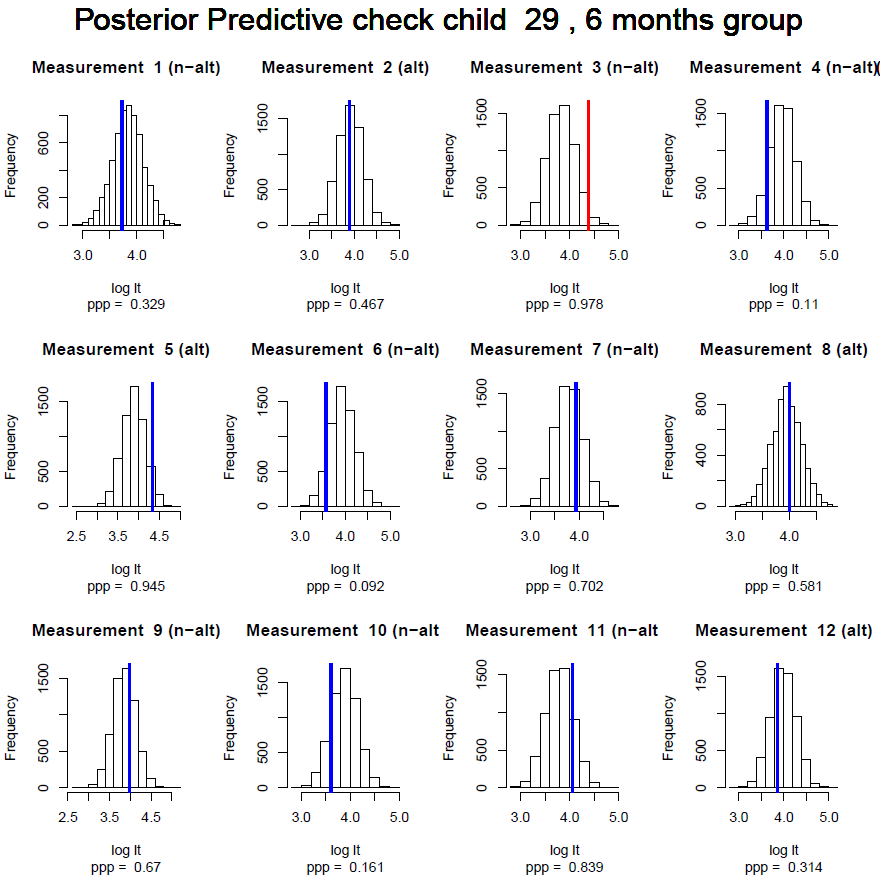
\includegraphics[width=0.9\linewidth]{figures/chapter_4/Figure9} 

}

\caption{Example of posterior predictive check. 1500 Samples are generated based on the model estimates for each measurement for each individual. The original observation is marked with a blue line if it falls within the 95\% interval of the observations and with red if it falls outside. If the model is a good model the observed data should not be surprising given the model. As such, if the model is good we should expect few observations that we cannot explain and thus few 'red' lines in the histograms. }\label{fig:ch04fig9}
\end{figure}

\begin{figure}

{\centering 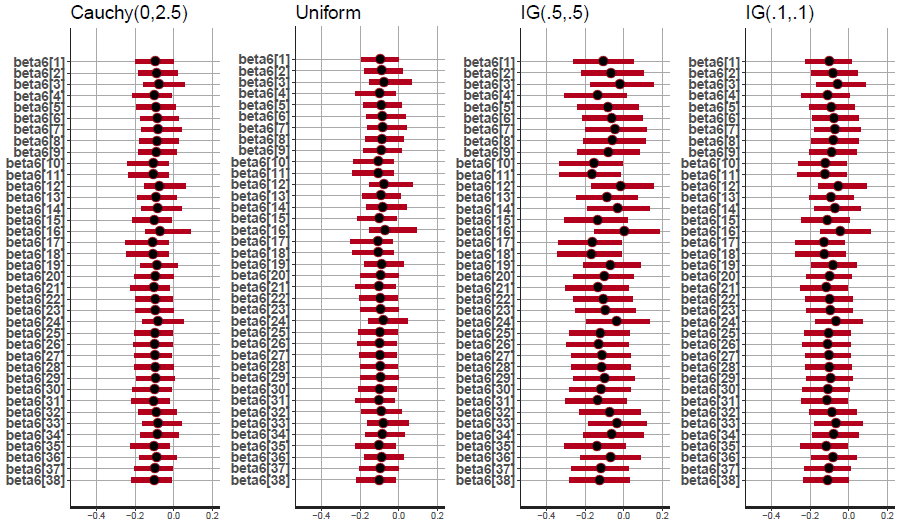
\includegraphics[width=0.85\linewidth]{figures/chapter_4/Figure10} 

}

\caption{Results of the sensitivity analyses regarding the effects of the choice of the prior on the group standard deviation parameters  on the condition parameter in which we a interested for this study.}\label{fig:ch04fig10}
\end{figure}

\begin{figure}

{\centering 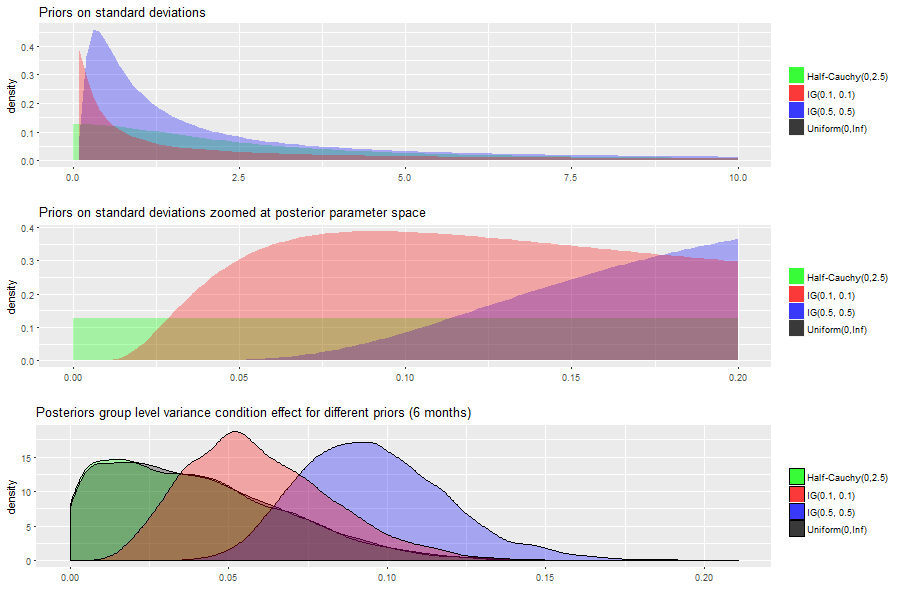
\includegraphics[width=0.85\linewidth]{figures/chapter_4/Figure11} 

}

\caption{Visualization of the priors used in the sensitivity analysis, also zoomed at the posterior parameter space that is relevant and we also present the resulting posterior distributions if these priors are used.}\label{fig:ch04fig11}
\end{figure}

\hypertarget{Burns}{%
\chapter{The importance of collaboration in Bayesian analyses with small samples}\label{Burns}}

\chaptermark{THE IMPORTANCE OF COLLABORATION}
\thispagestyle{empty}

\blfootnote{This chapter is accepted as Veen, D. \& Egberts, M. R. (2020). The importance of collaboration in Bayesian analyses with small samples. In R. Van de Schoot \& M. Miočević (Eds.), \textit{Small sample size solutions: A guide for applied researchers and practitioners}: Routledge.\\
\indent DV and ME wrote and revised this chapter together. DV conducted the statistical analyses. DV and ME interpreted the results together.}

\hypertarget{abstract-3}{%
\section*{Abstract}\label{abstract-3}}
\addcontentsline{toc}{section}{Abstract}

\small

This chapter addresses Bayesian estimation with (weakly) informative priors as a solution for small sample size issues. Special attention is paid to the problems that may arise in the analysis process, showing that Bayesian estimation should not be considered a quick solution for small sample size problems in complex models. The analysis steps are described and illustrated with an empirical example for which the planned analysis goes awry. Several solutions are presented for the problems that arise, and the chapter shows that different solutions can result in different posterior summaries and substantive conclusions. Therefore, statistical solutions should always be evaluated in the context of the substantive research question. This emphasizes the need for a constant interaction and collaboration between applied researchers and statisticians.

\normalsize
\newpage

\hypertarget{ch05introduction}{%
\section{Introduction}\label{ch05introduction}}

Complex statistical models, such as Structural Equation Models (SEMs), generally require large sample sizes (Tabachnick, Fidell, \& Ullman, \protect\hyperlink{ref-tabachnick_using_2007}{2007}; Wang \& Wang, \protect\hyperlink{ref-wang_structural_2012}{2012}). In practice, a large enough sample cannot always be easily obtained. Still, some research questions can only be answered with complex statistical models. Fortunately, solutions exist to overcome estimation issues with small sample sizes for complex models, see Smid et al. (\protect\hyperlink{ref-smid_bayesian_2019}{2019}\protect\hyperlink{ref-smid_bayesian_2019}{b}) for a systematic review comparing frequentist and Bayesian approaches . The current chapter addresses one of these solutions, namely Bayesian estimation with informative priors. In the process of Bayesian estimation, the WAMBS-checklist (When-to-Worry-and-How-to-Avoid-the-Misuse-of-Bayesian-Statistics; Depaoli \& Van de Schoot, \protect\hyperlink{ref-depaoli_improving_2017}{2017}) is a helpful tool; see also Schoot, Veen, Smeets, Winter, \& Depaoli (\protect\hyperlink{ref-van_de_schoot_tutorial_2020}{2020}). However, problems may arise in Bayesian analyses with informative priors, and whereas these problems are generally recognized in the field, they are not always described or solved in existing tutorials, statistical handbooks or example papers. This chapter offers an example of issues arising in the estimation of a Latent Growth Model (LGM) with a distal outcome using Bayesian methods with informative priors and a small data set of young children with burn injuries and their mothers. Moreover, we introduce two additional tools for diagnosing estimation issues: divergent transitions and the effective sample size of the posterior parameter samples, available in Stan (Stan Development Team, \protect\hyperlink{ref-stan_development_team_rstan:_2018}{2018}\protect\hyperlink{ref-stan_development_team_rstan:_2018}{b}) which makes use of an advanced Hamiltonian Monte Carlo (HMC) algorithm called the No-U-Turn-Sampler (NUTS: Hoffman \& Gelman, \protect\hyperlink{ref-hoffman_no-u-turn_2014}{2014}). These diagnostics can be used in addition to the checks described in the WAMBS checklist.

In the following sections, we briefly introduce LGMs and address the role of sample size, followed by an empirical example for which we present an analysis plan. Next, we show the process of adjusting the analysis in response to estimation problems. We show that different solutions can differentially impact the posterior summaries and substantive conclusions. This chapter highlights the importance of collaboration between substantive experts and statisticians when an initial analysis plan goes awry.

\hypertarget{latent-growth-models-with-small-sample-sizes}{%
\section{Latent Growth Models with small sample sizes}\label{latent-growth-models-with-small-sample-sizes}}

Latent Growth Models (LGMs) include repeated measurements of observed variables, and allow researchers to examine change over time in the construct of interest. LGMs can be extended to include distal outcomes and covariates (see Figure \ref{fig:ch05fig1}). One of the benefits of specifying an LGM as a structural equation model (SEM), as opposed to a multilevel model as discussed in Hox \& McNeish (\protect\hyperlink{ref-hox_small_2020}{2020}), is that growth can be specified as a non-monotonic or even non-linear function. For instance, we can specify an LGM in which part of the growth process is fixed and another part is estimated from the data. In Figure \ref{fig:ch05fig1}, two constraints on the relationships between the latent slope and measurement occasions are freed for two waves, thereby estimating \(\lambda_{22}\) and \(\lambda_{23}\) from the data. As a result, we allow individuals to differ in the way their manifest variables change from the first to the last measurement.

\begin{figure}

{\centering 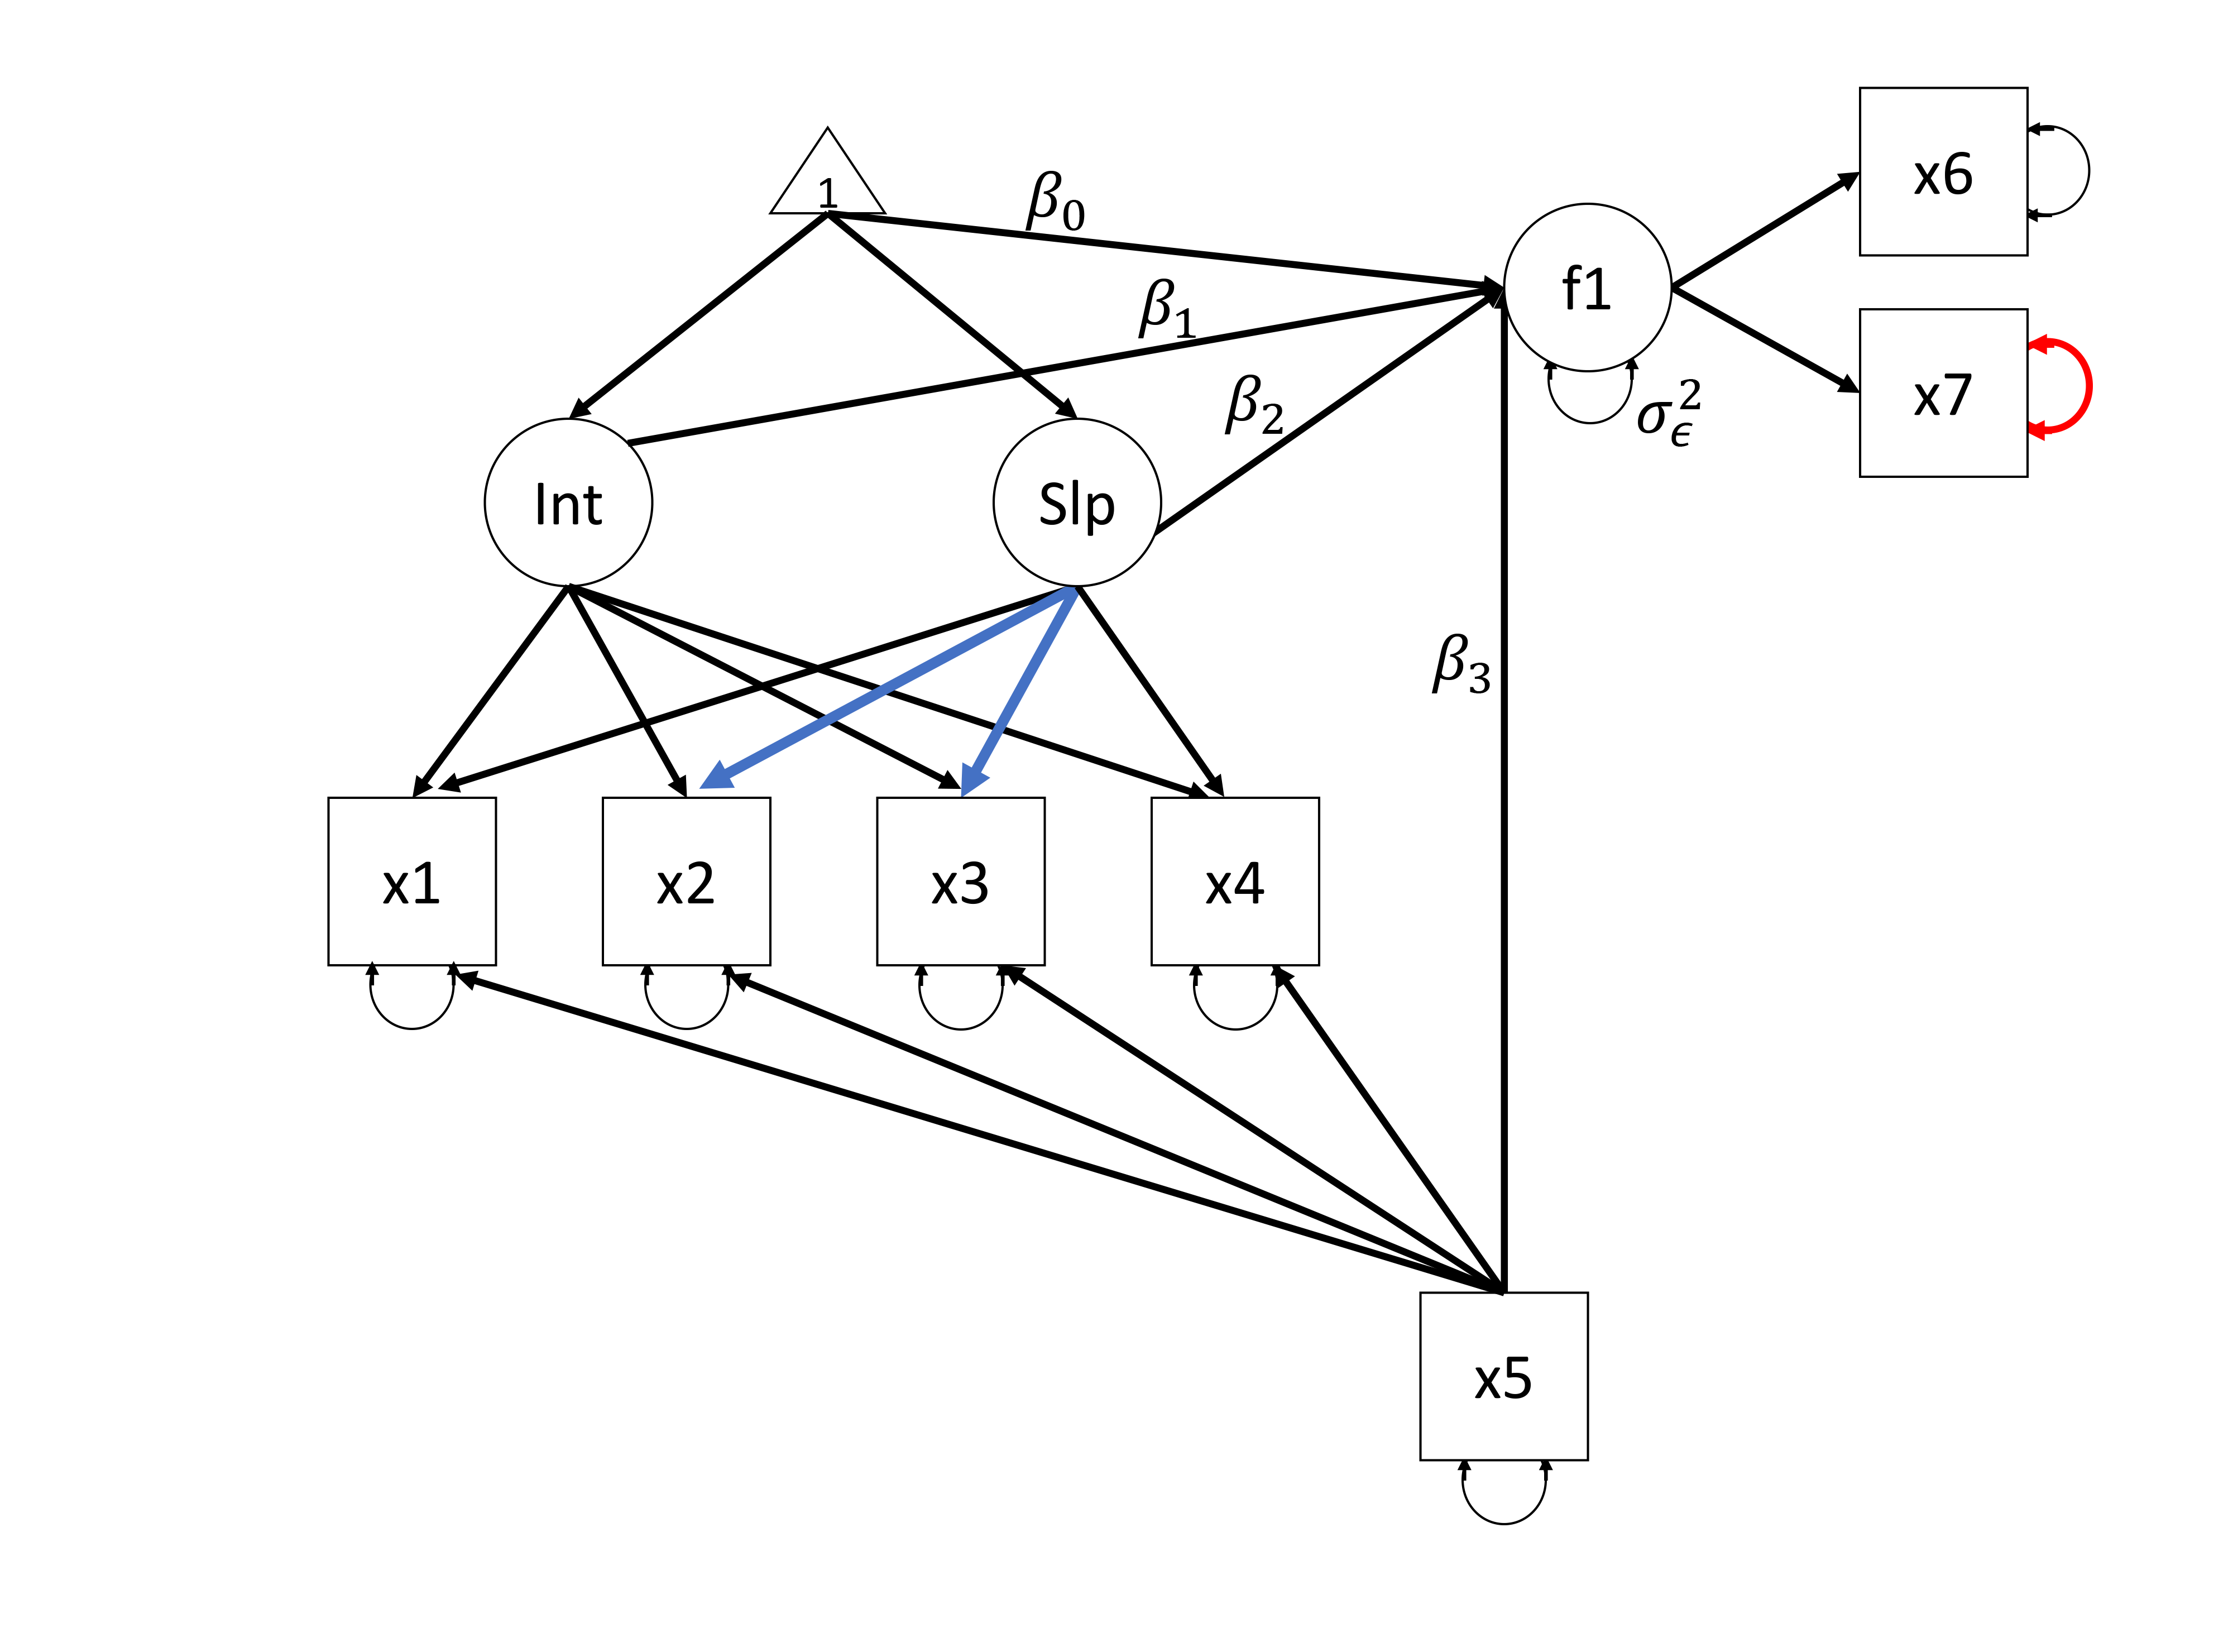
\includegraphics[width=0.8\linewidth]{figures/chapter_5/Figure1} 

}

\caption{The Latent Growth Model as used in the empirical example. The parameters of interest are the intercept of the latent factor f1 ($\beta_0$), f1 regressed on the latent intercept ($\beta_1$), the latent slope ($\beta_2$) and x5 ($\beta_3$) and the residual variance of the latent factor f1 ($\sigma_\epsilon^2$). The two blue factor loadings indicate freely estimated relationships for $\lambda_{22}$ and $\lambda_{23}$ (respectively). The red residual variance parameter ($\theta_{77}$) is highlighted throughout the empirical example. }\label{fig:ch05fig1}
\end{figure}

One drawback of LGMs, however, is that such models generally require large sample sizes. The more restrictions we place on a model, the fewer parameters there are to estimate, and the smaller the required sample size. The restrictions placed should, however, be in line with theory and research questions. Small sample sizes can cause problems such as high bias and low coverage (Hox \& Maas, \protect\hyperlink{ref-hox_accuracy_2001}{2001}), nonconvergence or improper solutions such as negative variance estimates (Wang \& Wang, \protect\hyperlink{ref-wang_structural_2012}{2012}, Chapter 7), and the question is how large should the sample size be to avoid these issues. Several simulation studies using maximum likelihood estimation have provided information on required sample sizes for SEM in general, and LGM specifically. To get an indication of the required sample size, we can use some rather arbitrary rules of thumb. Anderson \& Gerbing (\protect\hyperlink{ref-anderson_structural_1988}{1988}) recommend N = 100-150 for SEM in general. Hertzog, Oertzen, Ghisletta, \& Lindenberger (\protect\hyperlink{ref-hertzog_evaluating_2008}{2008}) investigated the power of LGM to detect individual differences in rate of change (i.e., the variance of the latent slope in LGMs). This is relevant for the model in Figure \ref{fig:ch05fig1} because the detection of these differences is needed if the individual rate of change over time (individual parameter estimates for the latent slope) is suitable to be used as a predictor in a regression analysis. In favorable simulation conditions (high Growth Curve Reliability, high correlation between intercept and slope, and many measurement occasions), maximum likelihood estimation has sufficient power to detect individual differences in change with N = 100. However, in unfavorable conditions even a sample size of 500 did not result in enough power to detect individual differences in change. Additionally, the model in the simulation studies by Hertzog and colleagues contained fewer parameters when compared to the LGM model used in the current chapter, thus suggesting that running the model in this chapter would require even larger sample sizes than those recommended by Hertzog and colleagues.

Bayesian estimation is often suggested as a solution for problems encountered in SEM with small sample sizes because it does not rely on the central limit theorem. A recent review examined the performance of Bayesian estimation in comparison to frequentist estimation methods for SEM in small samples on the basis of previously published simulation studies (Smid et al., \protect\hyperlink{ref-smid_bayesian_2019}{2019}\protect\hyperlink{ref-smid_bayesian_2019}{b}). It was concluded that Bayesian estimation could be regarded as a valid solution for small sample problems in terms of reducing bias and increasing coverage only when thoughtful priors were specified. In general, naive (i.e., flat or uninformative) priors resulted in high levels of bias. These findings highlight the importance of thoughtfully including prior information when using Bayesian estimation in the context of small samples. Specific simulation studies for LGMs can be found in papers by (McNeish, \protect\hyperlink{ref-mcneish_using_2016}{2016}\protect\hyperlink{ref-mcneish_using_2016}{a}, \protect\hyperlink{ref-mcneish_using_2016-1}{2016}\protect\hyperlink{ref-mcneish_using_2016-1}{b}; Smid et al., \protect\hyperlink{ref-smid_predicting_2019}{2019}\protect\hyperlink{ref-smid_predicting_2019}{a}; Van De Schoot, Broere, Perryck, Zondervan-Zwijnenburg, \& Van Loey, \protect\hyperlink{ref-van_de_schoot_analyzing_2015}{2015}; Zondervan-Zwijnenburg, Depaoli, Peeters, \& Schoot, \protect\hyperlink{ref-zondervan-zwijnenburg_pushing_2018}{2018}).

In general, it is difficult to label a sample size as small or large, and this can only be done with respect to the complexity of the model. In the remainder of this chapter we use the example of the extensive and quite complex LGM that can be seen in Figure \ref{fig:ch05fig1}. We show that with a sample that is small with respect to the complexity of this model, issues arise in the estimation process even with Bayesian estimation with thoughtful priors. Moreover, we provide details on diagnostics, debugging of the analysis and the search for appropriate solutions. We show the need for both statistical and content expertise to make the most of a complicated situation.

\newpage

\hypertarget{empirical-example-analysis-plan}{%
\section{Empirical example: Analysis plan}\label{empirical-example-analysis-plan}}

In practice, there are instances in which only small sample data are available, for example in the case of specific and naturally small or difficult to access populations. In these cases, collecting more data is not an option, and simplifying research questions and statistical models is also undesirable because this will not lead to an appropriate answer to the intended research questions. In this section we introduce an empirical example for which only a small data set was available, and at the same time the research question required the complicated model in Figure \ref{fig:ch05fig1}.

\hypertarget{research-question-model-specification-and-an-overview-of-data}{%
\subsection{Research question, model specification and an overview of data}\label{research-question-model-specification-and-an-overview-of-data}}

The empirical example comprises a longitudinal study of child and parental adjustment after a pediatric burn event. Pediatric burn injuries can have long-term consequences for the child's health-related quality of life (HRQL), in terms of physical, psychological and social functioning. In addition, a pediatric burn injury is a potentially traumatic event for parents, and parents may experience posttraumatic stress symptoms (PTSS; i.e., symptoms of re-experiencing, avoidance and arousal) as a result. Parents' PTSS could also impact the child's long-term HRQL. It is important to know whether the initial level of parental PTSS after the event or the development of symptoms is a better predictor of long-term child HRQL, since this may provide information about the appropriate timing of potential interventions. Therefore, the research question of interest was how the initial level and the development of mothers' posttraumatic stress symptoms (PTSS) over time predict the child's long-term health-related quality of life (HRQL).

In terms of statistical modelling, the research question required an LGM to model PTSS development and a measurement model for the distal outcome, namely, the child's HRQL. The full hypothesized model and the main parameters of interest, i.e.~the regression coefficients of the predictors for the child's HRQL, \(\beta_0\) for the intercept, \(\beta_1\) for HRQL regressed on the latent intercept, \(\beta_2\) for HRQL regressed on the latent slope, \(\beta_3\) for HRQL regressed on the covariate, percentage of Total Body Surface Area (TBSA) burned, and the residual variance \(\sigma_\epsilon^2\), are displayed in Figure \ref{fig:ch05fig1}.

Mothers reported on PTSS at four time points (up to 18 months) after the burn injury by filling out the Impact of Event Scale (IES; Horowitz, Wilner, \& Alvarez, \protect\hyperlink{ref-horowitz_impact_1979}{1979}). The total IES score from each of the four time points was used in the LGM. Eighteen months postburn, mothers completed the Health Outcomes Burn Questionnaire (HOBQ; Kazis et al., \protect\hyperlink{ref-kazis_development_2002}{2002}), which consists of 10 subscales. Based on a confirmatory factor analysis, these subscales were divided into three factors, i.e., Development, Behavior and Concern factors. For illustrative reasons, we only focus on the Behavior factor in the current chapter which was measured by just two manifest variables. TBSA was used to indicate burn severity; this is the proportion of the body that is affected by second- or third-degree burns and it was used as a covariate. For more detailed information about participant recruitment, procedures, and measurements see (Bakker, Van der Heijden, Van Son, \& Van Loey, \protect\hyperlink{ref-bakker_course_2013}{2013}).

Data from only 107 families was available. Even though data were collected in multiple burn centers across the Netherlands and Belgium over a prolonged period of time (namely 3 years), obtaining this sample size was already a challenge because of two main reasons. Firstly, the incidence of pediatric burns is relatively low. Yearly, around 160 children between the ages of 0 and 4 years old require hospitalization in a specialized Dutch burn center (Baar, Vloemans, Beerthuizen, Middelkoop, \& R3, \protect\hyperlink{ref-van_baar_epidemiologie_2015}{2015}). Secondly, the acute hospitalization period in which families were recruited to participate is extremely stressful. Participating in research in this demanding and emotional phase may be perceived as an additional burden by parents.

Still, we aimed to answer a research question that required the complex statistical model displayed in Figure \ref{fig:ch05fig1}. Therefore, we used Bayesian estimation with weakly informative priors to overcome the issues of small sample size estimation with ML-estimation, for which the model shown in Figure \ref{fig:ch05fig1} resulted in negative variance estimates.

\hypertarget{specifying-and-understanding-priors}{%
\subsection{Specifying and understanding priors}\label{specifying-and-understanding-priors}}

The specification of the priors is one of the essential elements of Bayesian analysis, especially when the sample size is small. Given the complexity of the LGM model relative to the sample size, prior information was incorporated to facilitate the estimation of the model (i.e., step 1 of the WAMBS-checklist). In addition to careful consideration of the plausible parameter space, we used previous results to inform the priors in our current model (Egberts, Van de Schoot, Geenen, \& Van Loey, \protect\hyperlink{ref-egberts_parents_2017}{2017}).

The prior for the mean of the latent intercept (\(\alpha_1\)) could be regarded as informative with respect to the location specification. The location parameter, or mean of the normally distributed prior \(N(\mu_0, \sigma_0^2)\), was based on the results of a previous study (Egberts et al., \protect\hyperlink{ref-egberts_parents_2017}{2017}, Table 1) and set at 26. If priors are based on information from previously published studies, it is important to reflect on the exchangeability of the prior and current study, see for instance Miočević, Levy, \& Savord (\protect\hyperlink{ref-miocevic_role_2020}{2020}). Exchangeability would indicate that the samples are drawn from the same population and a higher prior certainty can be used. To evaluate exchangeability, the characteristics of the sample and the data collection procedure were evaluated. Both studies used identical questionnaires and measurement intervals, and the data were collected in exactly the same burn centers. The main difference between the samples was the age of the children (i.e., age range in the current sample: 8 months-4 years; age range in the previous sample: 8-18 years), and related to that, the age of the mothers also differed (i.e., mean age in the current sample: 32 years; mean age in the previous sample: 42 years). Although generally, child age has not been associated with parents' PTSS after medical trauma (e.g., Landolt, Vollrath, Ribi, Gnehm, \& Sennhauser, \protect\hyperlink{ref-landolt_incidence_2003}{2003}), the two studies are not completely exchangeable as a results of the age difference. Therefore, additional uncertainty about the value of the parameter was specified by selecting a relatively high prior variance (see Table \ref{tab:ch05tab1}).

The priors for the regression coefficients are related to the expected scale of their associated parameters. For \(\beta_1\) a \(N(0,4)\) prior was specified, thereby allocating the most density mass on the plausible parameter space. Therefore, given the scale of the instruments used, and the parametrization of the factor score model, the latent factor scores can take on values between zero and 100. A regression coefficient of -4 or 4 would be extremely implausible. If our expected value of 26 is accurate for the intercept, this would change our predicted factor score by -104 or 104, respectively. This would constitute a change larger than the range of the construct.
For \(\beta_2\) in contrast, a \(N(0, 2500)\) prior was specified because small latent slope values, near the prior group mean of the latent slope of zero, should be allowed to have large impacts on the latent factor scores. For instance, a slope value of 0.1 could be associated with a drop of 50 in HRQL, resulting in a coefficient of -500. Figure \ref{fig:ch05fig2} shows what would have happened to the prior predictive distributions for the latent factor scores if a N(0,2500) prior was specified for \(\beta_1\) instead of the \(N(0, 4)\) prior, keeping all other priors constant. The prior predictive densities for the factor scores in panel B of Figure \ref{fig:ch05fig2} place far too much support on parts of the parameter space that are impossible. The factor scores can only take on values between zero and 100 in our model specification. For more information on prior predictive distributions, see for instance Schoot et al. (\protect\hyperlink{ref-van_de_schoot_tutorial_2020}{2020}).

\begin{figure}[H]

{\centering \includegraphics[width=0.9\linewidth]{figures/chapter_5/Figure2} 

}

\caption{The effect of changing a single prior in the model specification on the prior predictive distributions of the Latent Factor Scores. The prior for $\beta_1$ is changed from weakly informative (panel A; $N(0,4)$) to uninformative (panel B; $N(0,2500)$). }\label{fig:ch05fig2}
\end{figure}

\newpage

\footnotesize

\begin{longtable}[]{@{}ccc@{}}
\caption{\label{tab:ch05tab1} Priors and justification for all priors that are used in the analysis. \(N(.,.)\) is normal distribution with mean and variance \(N(\mu_0,\sigma_0^2)\), \(HN(\mu_0, \sigma_0^2)\) is half-normal distribution encompassing only the positive part of the parameter space, \(U(.,.)\) is uniform distribution with a lower bound and an upper bound. In Stan code the normal distribution is specified using a mean and standard deviation \(N\mu_0, \sigma_0)\), not a mean and variance \(N(\mu_0, \sigma_0^2)\). This is what causes the differences between the code in the data archive and this table.}\tabularnewline
\toprule
\begin{minipage}[b]{0.29\columnwidth}\centering
Parameter\strut
\end{minipage} & \begin{minipage}[b]{0.16\columnwidth}\centering
Prior\strut
\end{minipage} & \begin{minipage}[b]{0.45\columnwidth}\centering
Justification\strut
\end{minipage}\tabularnewline
\midrule
\endfirsthead
\toprule
\begin{minipage}[b]{0.29\columnwidth}\centering
Parameter\strut
\end{minipage} & \begin{minipage}[b]{0.16\columnwidth}\centering
Prior\strut
\end{minipage} & \begin{minipage}[b]{0.45\columnwidth}\centering
Justification\strut
\end{minipage}\tabularnewline
\midrule
\endhead
\begin{minipage}[t]{0.29\columnwidth}\centering
group mean of the latent
intercept (\(\alpha_1\))\strut
\end{minipage} & \begin{minipage}[t]{0.16\columnwidth}\centering
\(N(26, 400)\)\strut
\end{minipage} & \begin{minipage}[t]{0.45\columnwidth}\centering
Previous article on different
cohort (Egberts et al., \protect\hyperlink{ref-egberts_parents_2017}{2017}, Table 1)\strut
\end{minipage}\tabularnewline
\begin{minipage}[t]{0.29\columnwidth}\centering
group standard deviation
of the latent intercept
(\(\sigma_{Int}\))\strut
\end{minipage} & \begin{minipage}[t]{0.16\columnwidth}\centering
\(HN(0, 400)\)\strut
\end{minipage} & \begin{minipage}[t]{0.45\columnwidth}\centering
Allows values to cover entire
parameter space for IES\strut
\end{minipage}\tabularnewline
\begin{minipage}[t]{0.29\columnwidth}\centering
group mean of the latent
slope (\(\alpha_2\))\strut
\end{minipage} & \begin{minipage}[t]{0.16\columnwidth}\centering
\(N(0, 4)\)\strut
\end{minipage} & \begin{minipage}[t]{0.45\columnwidth}\centering
Allows values to cover entire
parameter space for IES\strut
\end{minipage}\tabularnewline
\begin{minipage}[t]{0.29\columnwidth}\centering
group standard deviation
of the latent slope
(\(\sigma_{slope}\))\strut
\end{minipage} & \begin{minipage}[t]{0.16\columnwidth}\centering
\(HN(0, 1)\)\strut
\end{minipage} & \begin{minipage}[t]{0.45\columnwidth}\centering
Allows values to cover entire
parameter space for IES\strut
\end{minipage}\tabularnewline
\begin{minipage}[t]{0.29\columnwidth}\centering
\(x1-x4\) regressed on
\(x5\) (\(\beta_{ies}\))\strut
\end{minipage} & \begin{minipage}[t]{0.16\columnwidth}\centering
\(N(0, 4)\)\strut
\end{minipage} & \begin{minipage}[t]{0.45\columnwidth}\centering
Allows values to cover entire
parameter space for IES\strut
\end{minipage}\tabularnewline
\begin{minipage}[t]{0.29\columnwidth}\centering
group mean relation IES
3 months (\(x2\)) regressed
on slope
(\(\mu_{\lambda_{22}}\))\strut
\end{minipage} & \begin{minipage}[t]{0.16\columnwidth}\centering
\(N(3, 25)\)\strut
\end{minipage} & \begin{minipage}[t]{0.45\columnwidth}\centering
Centered at 3 which would be the
constraint in a linear LGM.
Allowed to vary between individuals
to allow for between-person
differences in the way manifest
variables change from the first
to the last measurement\strut
\end{minipage}\tabularnewline
\begin{minipage}[t]{0.29\columnwidth}\centering
group mean relation
IES 12 months (\(x3\))
regressed on slope
(\(\mu_{\lambda_{23}}\))\strut
\end{minipage} & \begin{minipage}[t]{0.16\columnwidth}\centering
\(N(12, 25)\)\strut
\end{minipage} & \begin{minipage}[t]{0.45\columnwidth}\centering
Centered at 12 which would be the
constraint in a linear LGM.
Allowed to vary between individuals
to allow for between-person
differences in the way manifest
variables change from the first
to the last measurement.\strut
\end{minipage}\tabularnewline
\begin{minipage}[t]{0.29\columnwidth}\centering
group standard deviation
relation IES 3 months
(\(x2\)) regressed on slope
(\(\sigma_{\lambda_{22}}\))\strut
\end{minipage} & \begin{minipage}[t]{0.16\columnwidth}\centering
\(HN(0, 6.25)\)\strut
\end{minipage} & \begin{minipage}[t]{0.45\columnwidth}\centering
Allows for large and small
between-person differences in the
way manifest variables change from
the first to the last measurement.\strut
\end{minipage}\tabularnewline
\begin{minipage}[t]{0.29\columnwidth}\centering
group standard deviation
relation IES 12 months
(\(x3\)) regressed on slope
(\(\sigma_{\lambda_{23}}\))\strut
\end{minipage} & \begin{minipage}[t]{0.16\columnwidth}\centering
\(HN(0, 6.25)\)\strut
\end{minipage} & \begin{minipage}[t]{0.45\columnwidth}\centering
Allows for large and small
between-person differences in the
way manifest variables change from
the first to the last measurement.\strut
\end{minipage}\tabularnewline
\begin{minipage}[t]{0.29\columnwidth}\centering
All residual standard
deviations \(x1-x4\)
(\(\sigma_{\epsilon_{ies}}\))\strut
\end{minipage} & \begin{minipage}[t]{0.16\columnwidth}\centering
\(HN(0, 100)\)\strut
\end{minipage} & \begin{minipage}[t]{0.45\columnwidth}\centering
Allows values to cover entire
parameter space for the observed
variables\strut
\end{minipage}\tabularnewline
\begin{minipage}[t]{0.29\columnwidth}\centering
Intercepts factor
regressions (\(\beta_0\))\strut
\end{minipage} & \begin{minipage}[t]{0.16\columnwidth}\centering
\(N(50, 2500)\)\strut
\end{minipage} & \begin{minipage}[t]{0.45\columnwidth}\centering
Covers full factor score parameter
space centered at middle\strut
\end{minipage}\tabularnewline
\begin{minipage}[t]{0.29\columnwidth}\centering
Factors regressed on
Level (\(\beta_1\))\strut
\end{minipage} & \begin{minipage}[t]{0.16\columnwidth}\centering
\(N(0, 4)\)\strut
\end{minipage} & \begin{minipage}[t]{0.45\columnwidth}\centering
Allows values to cover entire
parameter space for the factor scores\strut
\end{minipage}\tabularnewline
\begin{minipage}[t]{0.29\columnwidth}\centering
Factors regressed on
Shape (\(\beta_2\))\strut
\end{minipage} & \begin{minipage}[t]{0.16\columnwidth}\centering
\(N(0, 2500)\)\strut
\end{minipage} & \begin{minipage}[t]{0.45\columnwidth}\centering
Allows values to cover entire
parameter space for the factor scores\strut
\end{minipage}\tabularnewline
\begin{minipage}[t]{0.29\columnwidth}\centering
Factors regressed on
TBSA (\(\beta_3\))\strut
\end{minipage} & \begin{minipage}[t]{0.16\columnwidth}\centering
\(N(0, 4)\)\strut
\end{minipage} & \begin{minipage}[t]{0.45\columnwidth}\centering
Allows values to cover entire
parameter space for the factor scores\strut
\end{minipage}\tabularnewline
\begin{minipage}[t]{0.29\columnwidth}\centering
Residual standard
deviation factors
(\(\sigma_\epsilon\))\strut
\end{minipage} & \begin{minipage}[t]{0.16\columnwidth}\centering
\(HN(0, 100)\)\strut
\end{minipage} & \begin{minipage}[t]{0.45\columnwidth}\centering
Allows values to cover entire
parameter space for the residuals\strut
\end{minipage}\tabularnewline
\bottomrule
\end{longtable}

\normalsize

\newpage

\hypertarget{empirical-example-conducting-the-analysis}{%
\section{Empirical example: Conducting the analysis}\label{empirical-example-conducting-the-analysis}}

Based on theoretical considerations, we specified the model as shown in Figure \ref{fig:ch05fig1} using the priors as specified in Table \ref{tab:ch05tab1}. We used Stan (Carpenter et al., \protect\hyperlink{ref-carpenter_stan:_2017}{2017}) via RStan (Stan Development Team, \protect\hyperlink{ref-stan_development_team_rstan:_2018}{2018}\protect\hyperlink{ref-stan_development_team_rstan:_2018}{b}) to estimate the model and we used the advanced version of the Hamiltonian Monte Carlo (HMC) algorithm called the No-U-Turn sampler (NUTS; Hoffman \& Gelman, \protect\hyperlink{ref-hoffman_no-u-turn_2014}{2014}). To run the model, we used the following code which by default ran the model using four chains with 2000 MCMC iterations of which 1000 are warmup samples:

\begin{Shaded}
\begin{Highlighting}[]
\NormalTok{fit_default <-}\StringTok{ }\KeywordTok{sampling}\NormalTok{(model, }\DataTypeTok{data =} \KeywordTok{list}\NormalTok{(}\DataTypeTok{X =}\NormalTok{ X, I, K, }
                                           \DataTypeTok{run_estimation =} \DecValTok{1}\NormalTok{),}
                        \DataTypeTok{seed =} \DecValTok{11}\NormalTok{,  }\DataTypeTok{show_messages =} \OtherTok{TRUE}\NormalTok{) }
\end{Highlighting}
\end{Shaded}

For reproducibility purposes, the OSF webpage \href{https://osf.io/am7pr/}{(https://osf.io/am7pr/)} includes all annotated Rstan code and the data.

Upon completion of the estimation, we received the following warnings from Rstan indicating severe issues with the estimation procedure:

\begin{verbatim}
Warning messages:
1: There were 676 divergent transitions after warmup. 
Increasing adapt_delta above 0.8 may help. See:
http://mc-stan.org/misc/warnings.html#divergent-transitions-after-warmup 
2: There were 16 transitions after warmup that exceeded the 
maximum treedepth. Increase max_treedepth above 10. See
http://mc-stan.org/misc/warnings.html#maximum-treedepth-exceeded 
3: There were 4 chains where the estimated 
Bayesian Fraction of Missing Information was low. 
See http://mc-stan.org/misc/warnings.html#bfmi-low 
4: Examine the pairs() plot to diagnose sampling problems
\end{verbatim}

Fortunately, the warning messages also pointed to online resources with more detailed information about the problems. In what follows, we describe two diagnostics to detect issues in the estimation procedure: divergent transitions (this section) and the effective sample size of the MCMC algorithm (next section).

The most important warning message is about divergent transitions (warning message 1). The appearance of divergent transitions is a strong indicator that the posterior results as shown in column 1 of Table \ref{tab:ch05tab3} cannot be trusted (Stan Development Team, \protect\hyperlink{ref-stan_development_team_stan_2019}{2019}, Chapter 14). For detailed, highly technical information on this diagnostic, see Betancourt (\protect\hyperlink{ref-betancourt_diagnosing_2016}{2016}). Very loosely formulated, the occurrence of many divergent transitions indicates that there is something going wrong in drawing MCMC samples from the posterior. When the estimator moves from one iteration to the next, it does so using a particular step size. The larger steps the estimator can take between iterations, the more effectively it can explore the parameter space of the posterior distribution (compare Figure \ref{fig:ch05fig3}A with \ref{fig:ch05fig3}B). When a divergent transition occurs, the step size is too large to efficiently explore part of the posterior distribution and the sampler runs into problems when transitioning from one iteration to the next, (see Figure \ref{fig:ch05fig3}C). The Stan Development Team uses the following analogy to provide some intuition for the problem:

\begin{quote}
``For some intuition, imagine walking down a steep mountain. If you take too big of a step you will fall, but if you can take very tiny steps you might be able to make your way down the mountain, albeit very slowly. Similarly, we can tell Stan to take smaller steps around the posterior distribution, which (in some but not all cases) can help avoid these divergences.''

Stan Development Team (\protect\hyperlink{ref-stan_development_team_brief_2018}{2018}\protect\hyperlink{ref-stan_development_team_brief_2018}{a})
\end{quote}

The posterior results for the parameters of interest (\(\beta_0, \beta_1, \beta_2, \beta_3, \sigma_\epsilon\)) are shown in Table \ref{tab:ch05tab3}, column 1. Note that these results cannot be trusted and should not be interpreted because of the many divergent transitions. Divergent transitions can sometimes be resolved by simply taking smaller steps (see next section), which increases computational time.



\begin{figure}

{\centering 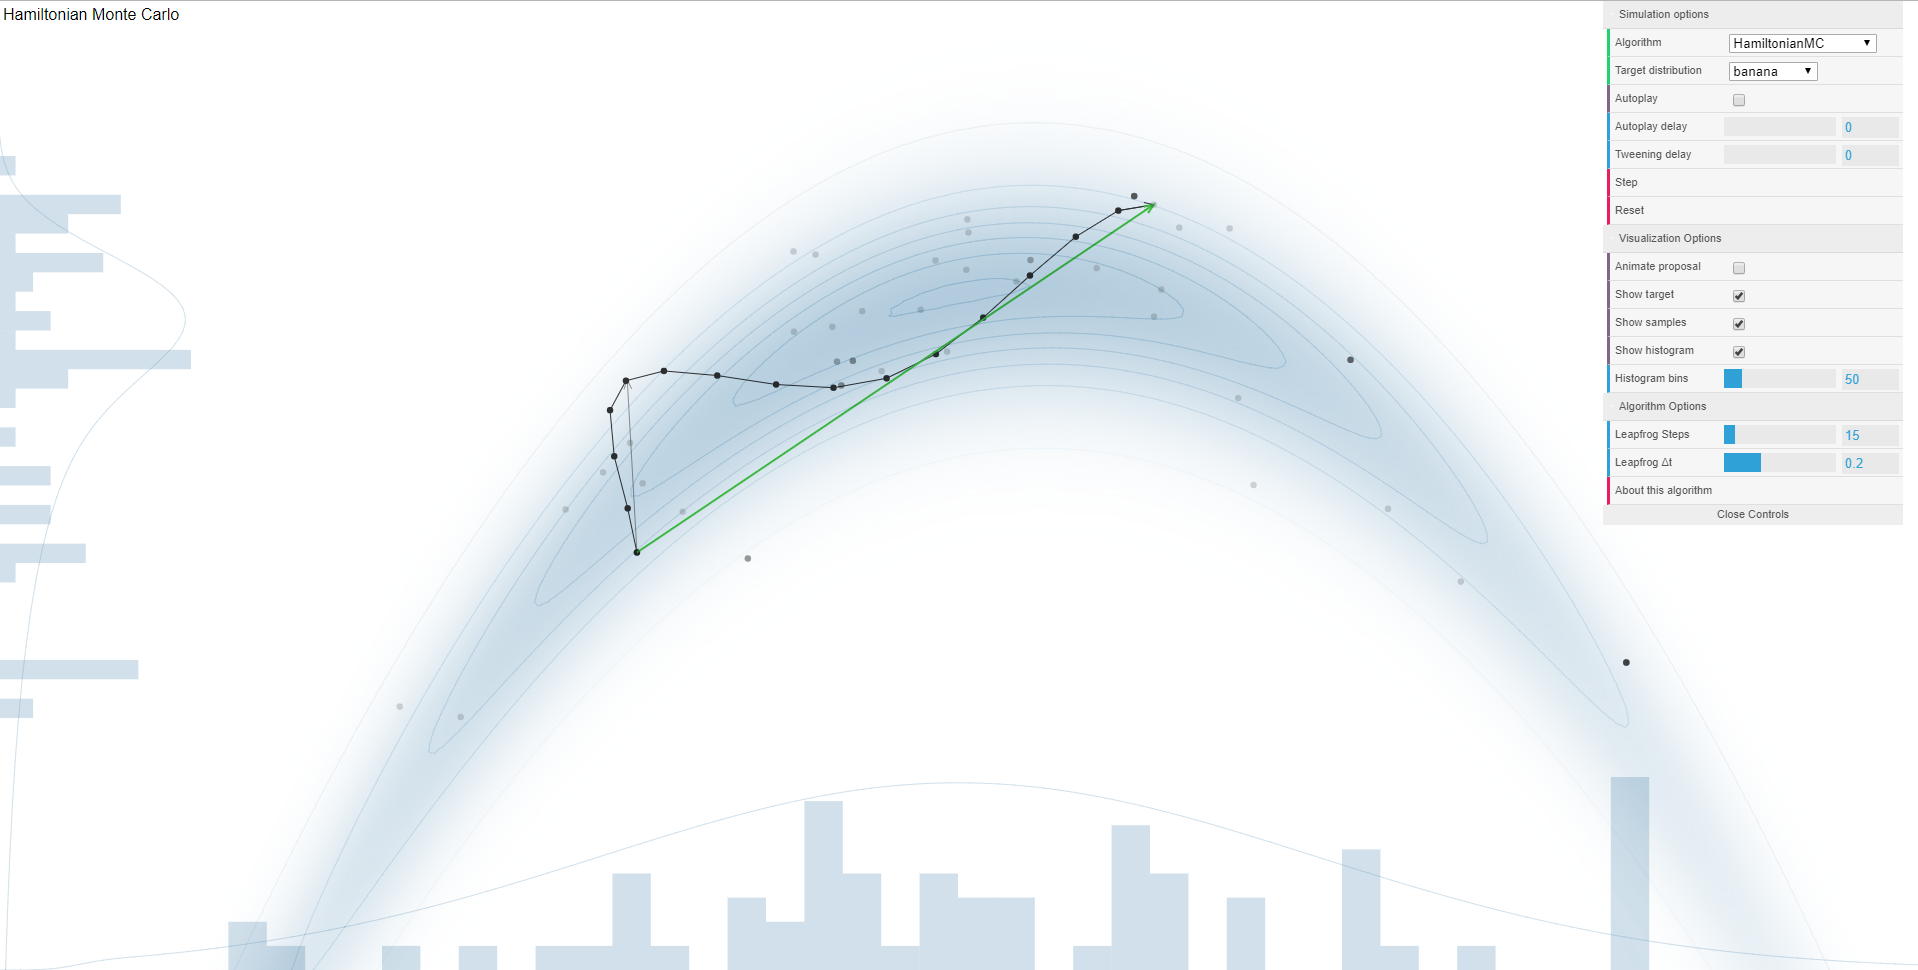
\includegraphics[width=0.7\linewidth]{C:/Users/Administrator/Dropbox/Werk/PhD UU/Dissertation/figures/chapter_5/Figure3/Figure3A} 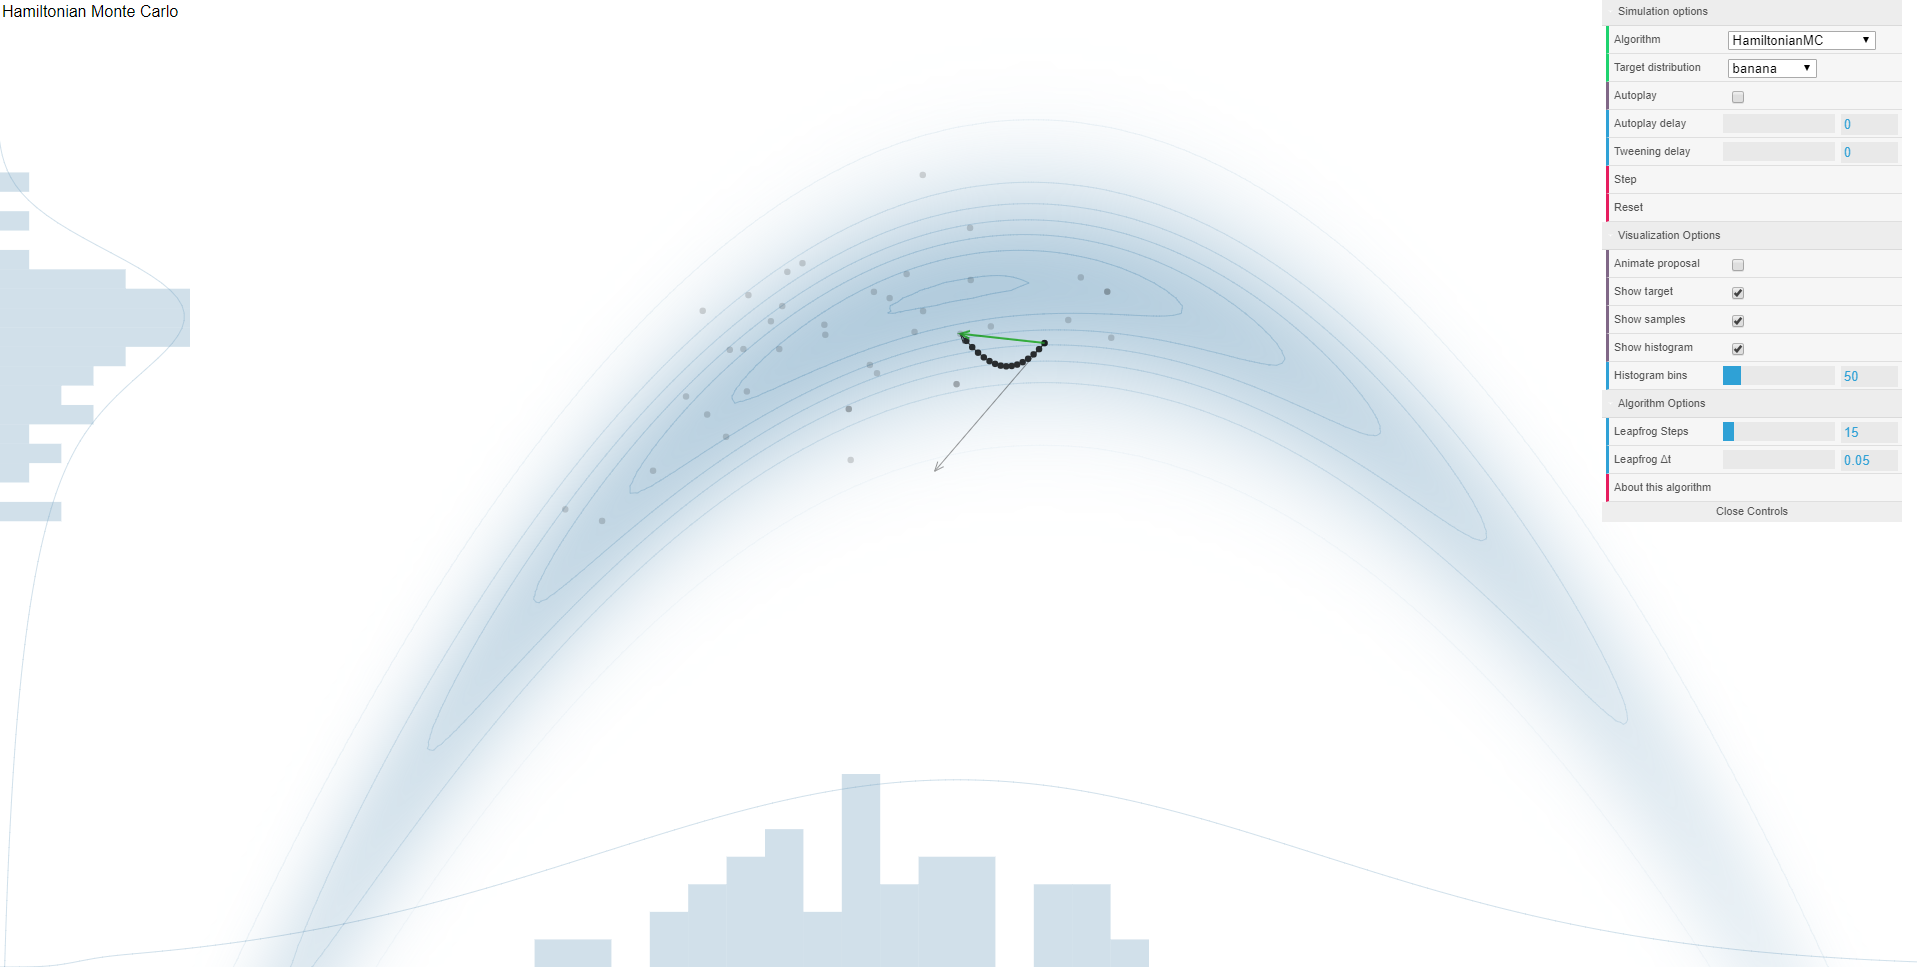
\includegraphics[width=0.7\linewidth]{C:/Users/Administrator/Dropbox/Werk/PhD UU/Dissertation/figures/chapter_5/Figure3/Figure3B} 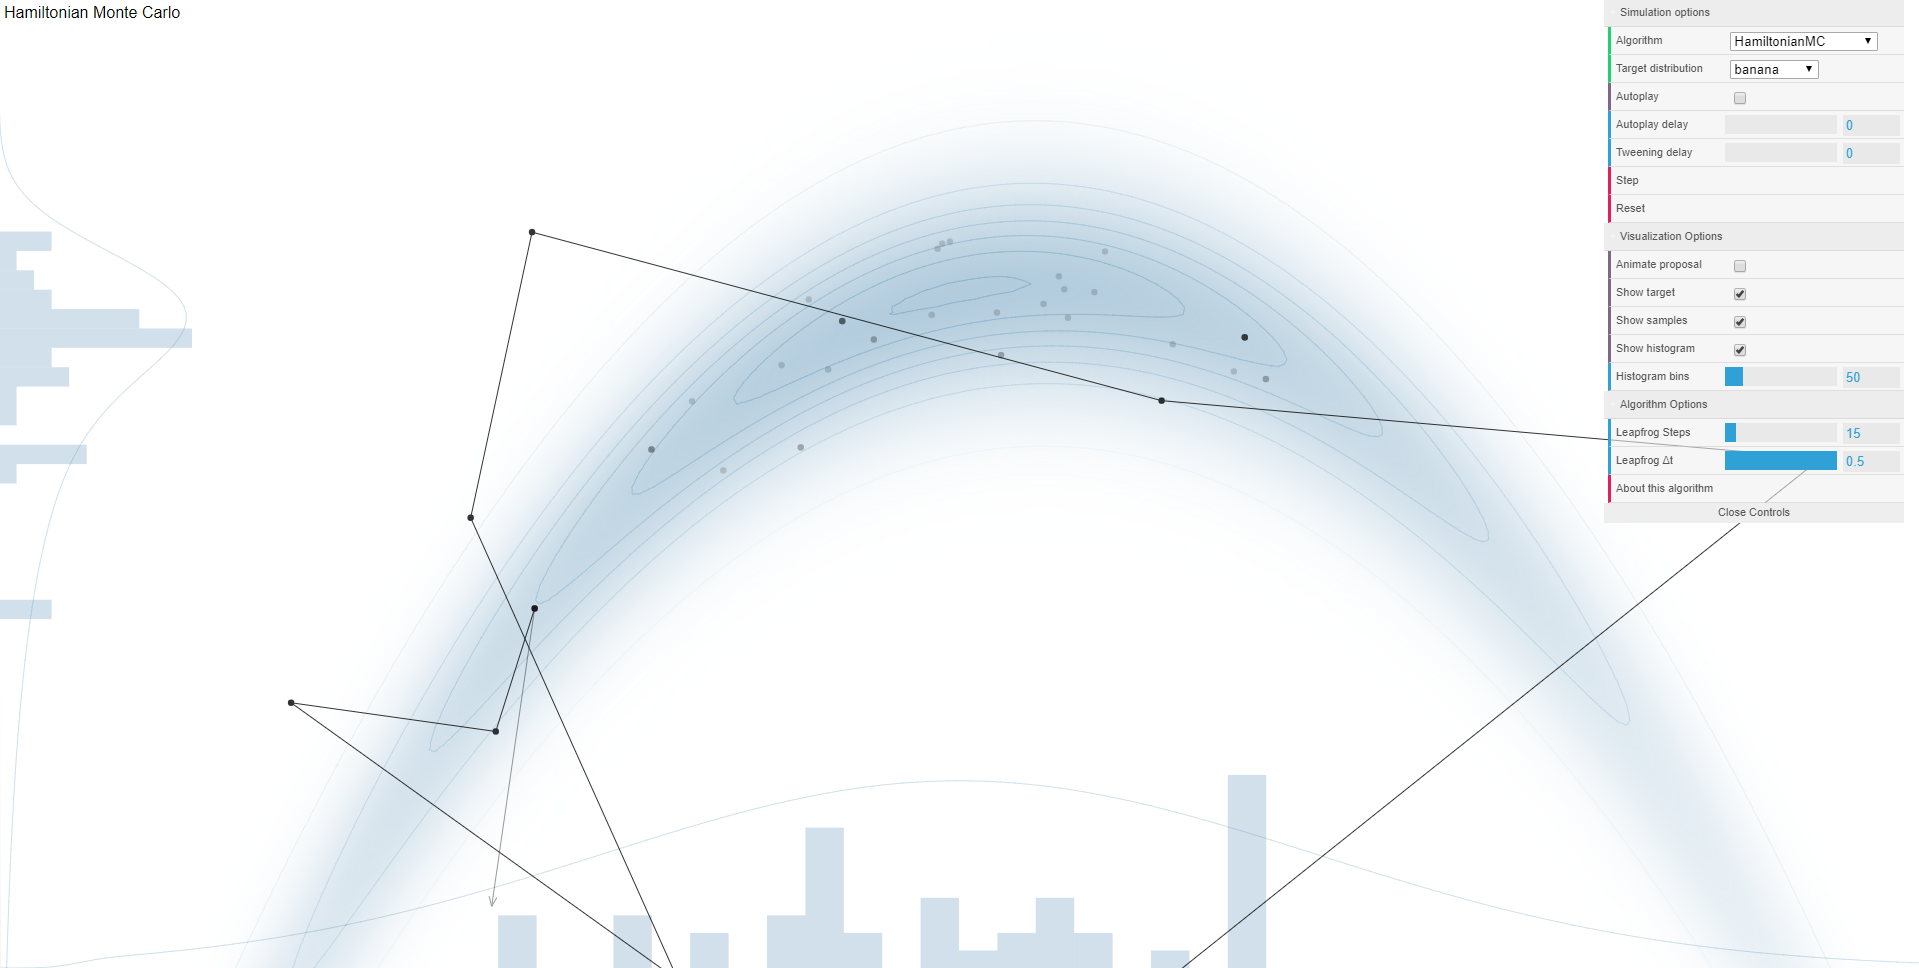
\includegraphics[width=0.7\linewidth]{C:/Users/Administrator/Dropbox/Werk/PhD UU/Dissertation/figures/chapter_5/Figure3/Figure3C} 

}

\caption{Effect of decreasing the step size of the HMC on the efficiency of the exploration of the posterior distribution (Panel A and B). The green arrow shows the step between two consecutive iterations. Panel A uses a large step size and swiftly samples from both posterior distributions, one of which is a normal distribution and one of which a common distributional form for variance parameters. Panel B, in contrast, needs more time to sample from both distributions and describe them accurately because the steps are a lot smaller in between iterations. Panel C shows an example of a divergent transition, which is indicative of problems with the sampling algorithm. These screenshots come from an application developed by Feng (\protect\hyperlink{ref-feng_markov-chain_2016}{2016}) that provides insight into different Bayesian sampling algorithms and their behavior for different shapes of posterior distributions.}\label{fig:ch05fig3}
\end{figure}

\hypertarget{debugging}{%
\section{Debugging}\label{debugging}}

The occurrence of divergent transitions can also be an indication of more serious issues with the model or with a specific parameter. One of the ways to find out which parameter might be problematic is to inspect how efficiently the sampler sampled from the posterior of each parameter. The efficiency of the sampling process can be expressed as the Effective Sample Size (ESS) for each parameter, where sample size does not refer to the data but to the samples taken from the posterior. In the default setting we saved 1000 of these samples per chain, so in total we obtained 4000 MCMC samples for each parameter. However, these MCMC samples are related to each other, which can be expressed by the degree of autocorrelation (point 5 on the WAMBS checklist in Chapter 3). ESS expresses how many independent MCMC samples are equivalent to the autocorrelated MCMC samples that were drawn. If a small ESS for a certain parameter is obtained, there is little information available to construct the posterior distribution of that parameter. This will also manifest itself in the form of autocorrelation and non-smooth histograms of posteriors. For more details on ESS and how RStan calculates it, see the Stan Reference Manual (Stan Development Team, \protect\hyperlink{ref-stan_development_team_stan_2019}{2019}).

In Table \ref{tab:ch05tab2} we provide the ESS for \(\alpha_1, \beta_1, \theta_{77}\) and the factor score of mother and child pair no. 33 (denoted by \(fs_{33}\)).\(fs_{33}\) was estimated efficiently and the ESS was 60\% of the number of MCMC samples, followed by \(\alpha_1\) (14\%) and \(\beta_1\) (11\%). \(\theta_{77}\), in contrast, had an ESS of only 0.5\% of the number of MCMC samples indicating an equivalence of only 20 MCMC samples had been used to construct the posterior distribution. There is no clear cut-off value for the ESS, although it is obvious that higher values are better and that 20 is very low. The default diagnostic threshold used in the R package shinystan (Gabry, \protect\hyperlink{ref-gabry_shinystan:_2018}{2018}), used for interactive visual and numerical diagnostics, is set to 10\%.

The effects of ESS on the histograms of these four parameters can be seen in Figure \ref{fig:ch05fig4} which shows a smooth distribution for \(fs_{33}\) but not for \(\theta_{77}\). Based on the ESS and the inspection of Figure \ref{fig:ch05fig4}, the residual variance parameter \(\theta_{77}\) was estimated with the lowest efficiency and probably exhibited the most issues in model estimation.

\blandscape

\begin{longtable}[]{@{}ccccccc@{}}
\caption{\label{tab:ch05tab2} Examples of Effective Sample Size (ESS) per parameter for the different model and estimation settings we used. Each column represents a different model, and each row represents a different variable. We report ESS with the corresponding percentage of the total number of iterations that was used to estimate that particular model in brackets. Note that with the highly efficient NUTS sampling algorithm a higher efficiency can be obtained compared to independent MC samples (Stan Development Team, \protect\hyperlink{ref-stan_development_team_stan_2019}{2019}, Chapter 15).}\tabularnewline
\toprule
\begin{minipage}[b]{0.08\columnwidth}\centering
Parameter\strut
\end{minipage} & \begin{minipage}[b]{0.13\columnwidth}\centering
Model with default
estimation settings\strut
\end{minipage} & \begin{minipage}[b]{0.14\columnwidth}\centering
Model with small
step size in
estimation setting\strut
\end{minipage} & \begin{minipage}[b]{0.10\columnwidth}\centering
Alternative I:
Remove perfect
HRQL scores\strut
\end{minipage} & \begin{minipage}[b]{0.11\columnwidth}\centering
Alternative II:
\(IG(0.5, 0.5)\)
prior for
\(\theta_{77}\)\strut
\end{minipage} & \begin{minipage}[b]{0.12\columnwidth}\centering
Alternative III:
Replace factor
score with \(x7\)\strut
\end{minipage} & \begin{minipage}[b]{0.12\columnwidth}\centering
Alternative IV:
Possible increase
of variance in
latent factor\strut
\end{minipage}\tabularnewline
\midrule
\endfirsthead
\toprule
\begin{minipage}[b]{0.08\columnwidth}\centering
Parameter\strut
\end{minipage} & \begin{minipage}[b]{0.13\columnwidth}\centering
Model with default
estimation settings\strut
\end{minipage} & \begin{minipage}[b]{0.14\columnwidth}\centering
Model with small
step size in
estimation setting\strut
\end{minipage} & \begin{minipage}[b]{0.10\columnwidth}\centering
Alternative I:
Remove perfect
HRQL scores\strut
\end{minipage} & \begin{minipage}[b]{0.11\columnwidth}\centering
Alternative II:
\(IG(0.5, 0.5)\)
prior for
\(\theta_{77}\)\strut
\end{minipage} & \begin{minipage}[b]{0.12\columnwidth}\centering
Alternative III:
Replace factor
score with \(x7\)\strut
\end{minipage} & \begin{minipage}[b]{0.12\columnwidth}\centering
Alternative IV:
Possible increase
of variance in
latent factor\strut
\end{minipage}\tabularnewline
\midrule
\endhead
\begin{minipage}[t]{0.08\columnwidth}\centering
\(fs_{33}\)\strut
\end{minipage} & \begin{minipage}[t]{0.13\columnwidth}\centering
2390 (60\%)\strut
\end{minipage} & \begin{minipage}[t]{0.14\columnwidth}\centering
9843 (123\%)\strut
\end{minipage} & \begin{minipage}[t]{0.10\columnwidth}\centering
2219 (55\%)\strut
\end{minipage} & \begin{minipage}[t]{0.11\columnwidth}\centering
1307 (33\%)\strut
\end{minipage} & \begin{minipage}[t]{0.12\columnwidth}\centering
-\strut
\end{minipage} & \begin{minipage}[t]{0.12\columnwidth}\centering
2485 (62\%)\strut
\end{minipage}\tabularnewline
\begin{minipage}[t]{0.08\columnwidth}\centering
\(\alpha_1\)\strut
\end{minipage} & \begin{minipage}[t]{0.13\columnwidth}\centering
575 (14\%)\strut
\end{minipage} & \begin{minipage}[t]{0.14\columnwidth}\centering
1000 (13\%)\strut
\end{minipage} & \begin{minipage}[t]{0.10\columnwidth}\centering
655 (16\%)\strut
\end{minipage} & \begin{minipage}[t]{0.11\columnwidth}\centering
145 (4\%)\strut
\end{minipage} & \begin{minipage}[t]{0.12\columnwidth}\centering
227 (6\%)\strut
\end{minipage} & \begin{minipage}[t]{0.12\columnwidth}\centering
611 (15\%)\strut
\end{minipage}\tabularnewline
\begin{minipage}[t]{0.08\columnwidth}\centering
\(\beta_1\)\strut
\end{minipage} & \begin{minipage}[t]{0.13\columnwidth}\centering
424 (11\%)\strut
\end{minipage} & \begin{minipage}[t]{0.14\columnwidth}\centering
1966 (25\%)\strut
\end{minipage} & \begin{minipage}[t]{0.10\columnwidth}\centering
487 (12\%)\strut
\end{minipage} & \begin{minipage}[t]{0.11\columnwidth}\centering
647 (16\%)\strut
\end{minipage} & \begin{minipage}[t]{0.12\columnwidth}\centering
58 (1\%)\strut
\end{minipage} & \begin{minipage}[t]{0.12\columnwidth}\centering
1004 (25\%)\strut
\end{minipage}\tabularnewline
\begin{minipage}[t]{0.08\columnwidth}\centering
\(\theta_{77}\)\strut
\end{minipage} & \begin{minipage}[t]{0.13\columnwidth}\centering
20 (0.5\%)\strut
\end{minipage} & \begin{minipage}[t]{0.14\columnwidth}\centering
12 (0.2\%)\strut
\end{minipage} & \begin{minipage}[t]{0.10\columnwidth}\centering
9 (0.2\%)\strut
\end{minipage} & \begin{minipage}[t]{0.11\columnwidth}\centering
33 (0.8\%)\strut
\end{minipage} & \begin{minipage}[t]{0.12\columnwidth}\centering
-\strut
\end{minipage} & \begin{minipage}[t]{0.12\columnwidth}\centering
46 (1.2\%)\strut
\end{minipage}\tabularnewline
\bottomrule
\end{longtable}

\elandscape

To investigate if there were systematic patterns in the divergences, we plotted the samples of the parameters \(fs_{33}\) and \(\theta_{77}\) against the log posterior (denoted by \(lp\)) (see Figure \ref{fig:ch05fig5}). \(lp\) is, very loosely formulated, an indication of the likelihood of the data given all posterior parameters. \(lp\) is sampled for each MCMC iteration as just another parameter. Note that, in contrast to log-likelihoods, \(lp\) cannot be used for model comparison. Plots such as those in Figure \ref{fig:ch05fig5} can point us to systematic patterns for the divergent transitions, which would indicate that a particular part of the parameter space is hard to explore. In Figure \ref{fig:ch05fig5}A it can be seen that for \(fs_{33}\), which did not exhibit problems in terms of ESS, the divergent transitions are more or less randomly distributed across the posterior parameter space. Also, the traceplot and histogram for \(fs_{33}\) would pass the WAMBS-checklist on initial inspection. There is one hotspot around the value of -1700 for the \(lp\) where a cluster of divergent transitions occurs. This is also visible in the traceplot, where it can be seen that one of the chains is stuck and fails to efficiently explore the parameter space shown as an almost horizontal line for many iterations. On closer inspection, a similar behavior in one of the chains could be seen for \(fs_{33}\) as well.

In Figure \ref{fig:ch05fig5}B it can be seen that for \(\theta_{77}\), which exhibited problems in terms of ESS, the divergent transitions occur mainly in a very specific part of the posterior parameter space, i.e., many divergent transitions occur close to zero. This also shows up in the traceplot, where for several iterations the sampler could not move away from zero. This indicates that our sampling algorithm ran into problems when exploring the possibility that \(\theta_{77}\) might be near zero. Note that a similar issue arises in one chain around the value of 2.5 for many iterations, resulting in a hot spot which corresponds to the deviant chain for \(lp\). Perhaps an additional parameter could be found which explains the issues concerning this systematic pattern of divergent transitions. For now, we continued with a focus on \(\theta_{77}\).

The first solution, also offered in the warning message provided by Stan, was to force Stan to use a smaller step size by increasing the \emph{adapt\_delta} setting of the estimator. We also deal with the second warning by increasing \emph{max\_treedepth}, although this is related to efficiency and not an indication of model error and validity issues. To make sure we could still explore the entire posterior parameter space, we extended the number of iterations post warmup to 2000 for each chain (\texttt{iter\ –\ warmup} in the code below). We used the following R code:

\begin{Shaded}
\begin{Highlighting}[]
\NormalTok{fit_small_step <-}\StringTok{ }\KeywordTok{sampling}\NormalTok{(model, }
                           \DataTypeTok{data=}\KeywordTok{list}\NormalTok{(}\DataTypeTok{X =}\NormalTok{ X, I, K, }\DataTypeTok{run_estimation =} \DecValTok{1}\NormalTok{),}
                           \DataTypeTok{control=}\KeywordTok{list}\NormalTok{(}\DataTypeTok{adapt_delta =} \FloatTok{.995}\NormalTok{,}
                                        \DataTypeTok{max_treedepth =} \DecValTok{16}\NormalTok{),}
                           \DataTypeTok{warmup =} \DecValTok{3000}\NormalTok{, }\DataTypeTok{iter =} \DecValTok{5000}\NormalTok{, }\DataTypeTok{seed =} \DecValTok{11235813}\NormalTok{) }
\end{Highlighting}
\end{Shaded}

We inspected the ESS for the same parameters again, which can be seen in Table \ref{tab:ch05tab2}. The problems seem to occur for the \(\theta_{77}\) parameter again, and it has even decreased in efficiency. We compared the posterior for \(\theta_{77}\) and \(lp\) between the default estimation settings and the estimation settings forcing a smaller step size in Figure \ref{fig:ch05fig6}. The smaller step sizes have decreased the number of divergent transitions to almost zero. Also, they enabled more exploration of posterior parameter values near zero. However, the posterior distribution still showed signs of problematic exploration given the strange pattern of MCMC samples close to 0.5 (see step 6 of the WAMBS checklist; do posterior estimates make substantive sense?). Apparently, the solution offered by the Rstan warning message to decrease the step size, which often solves the issue of obtaining divergent transitions, failed to provide an efficient result in this case. Thus the posterior estimates in Table \ref{tab:ch05tab3}, column 2 still cannot be trusted. In the next section, we briefly explore different solutions that might help us to obtain trustworthy results.

\begin{figure}

{\centering 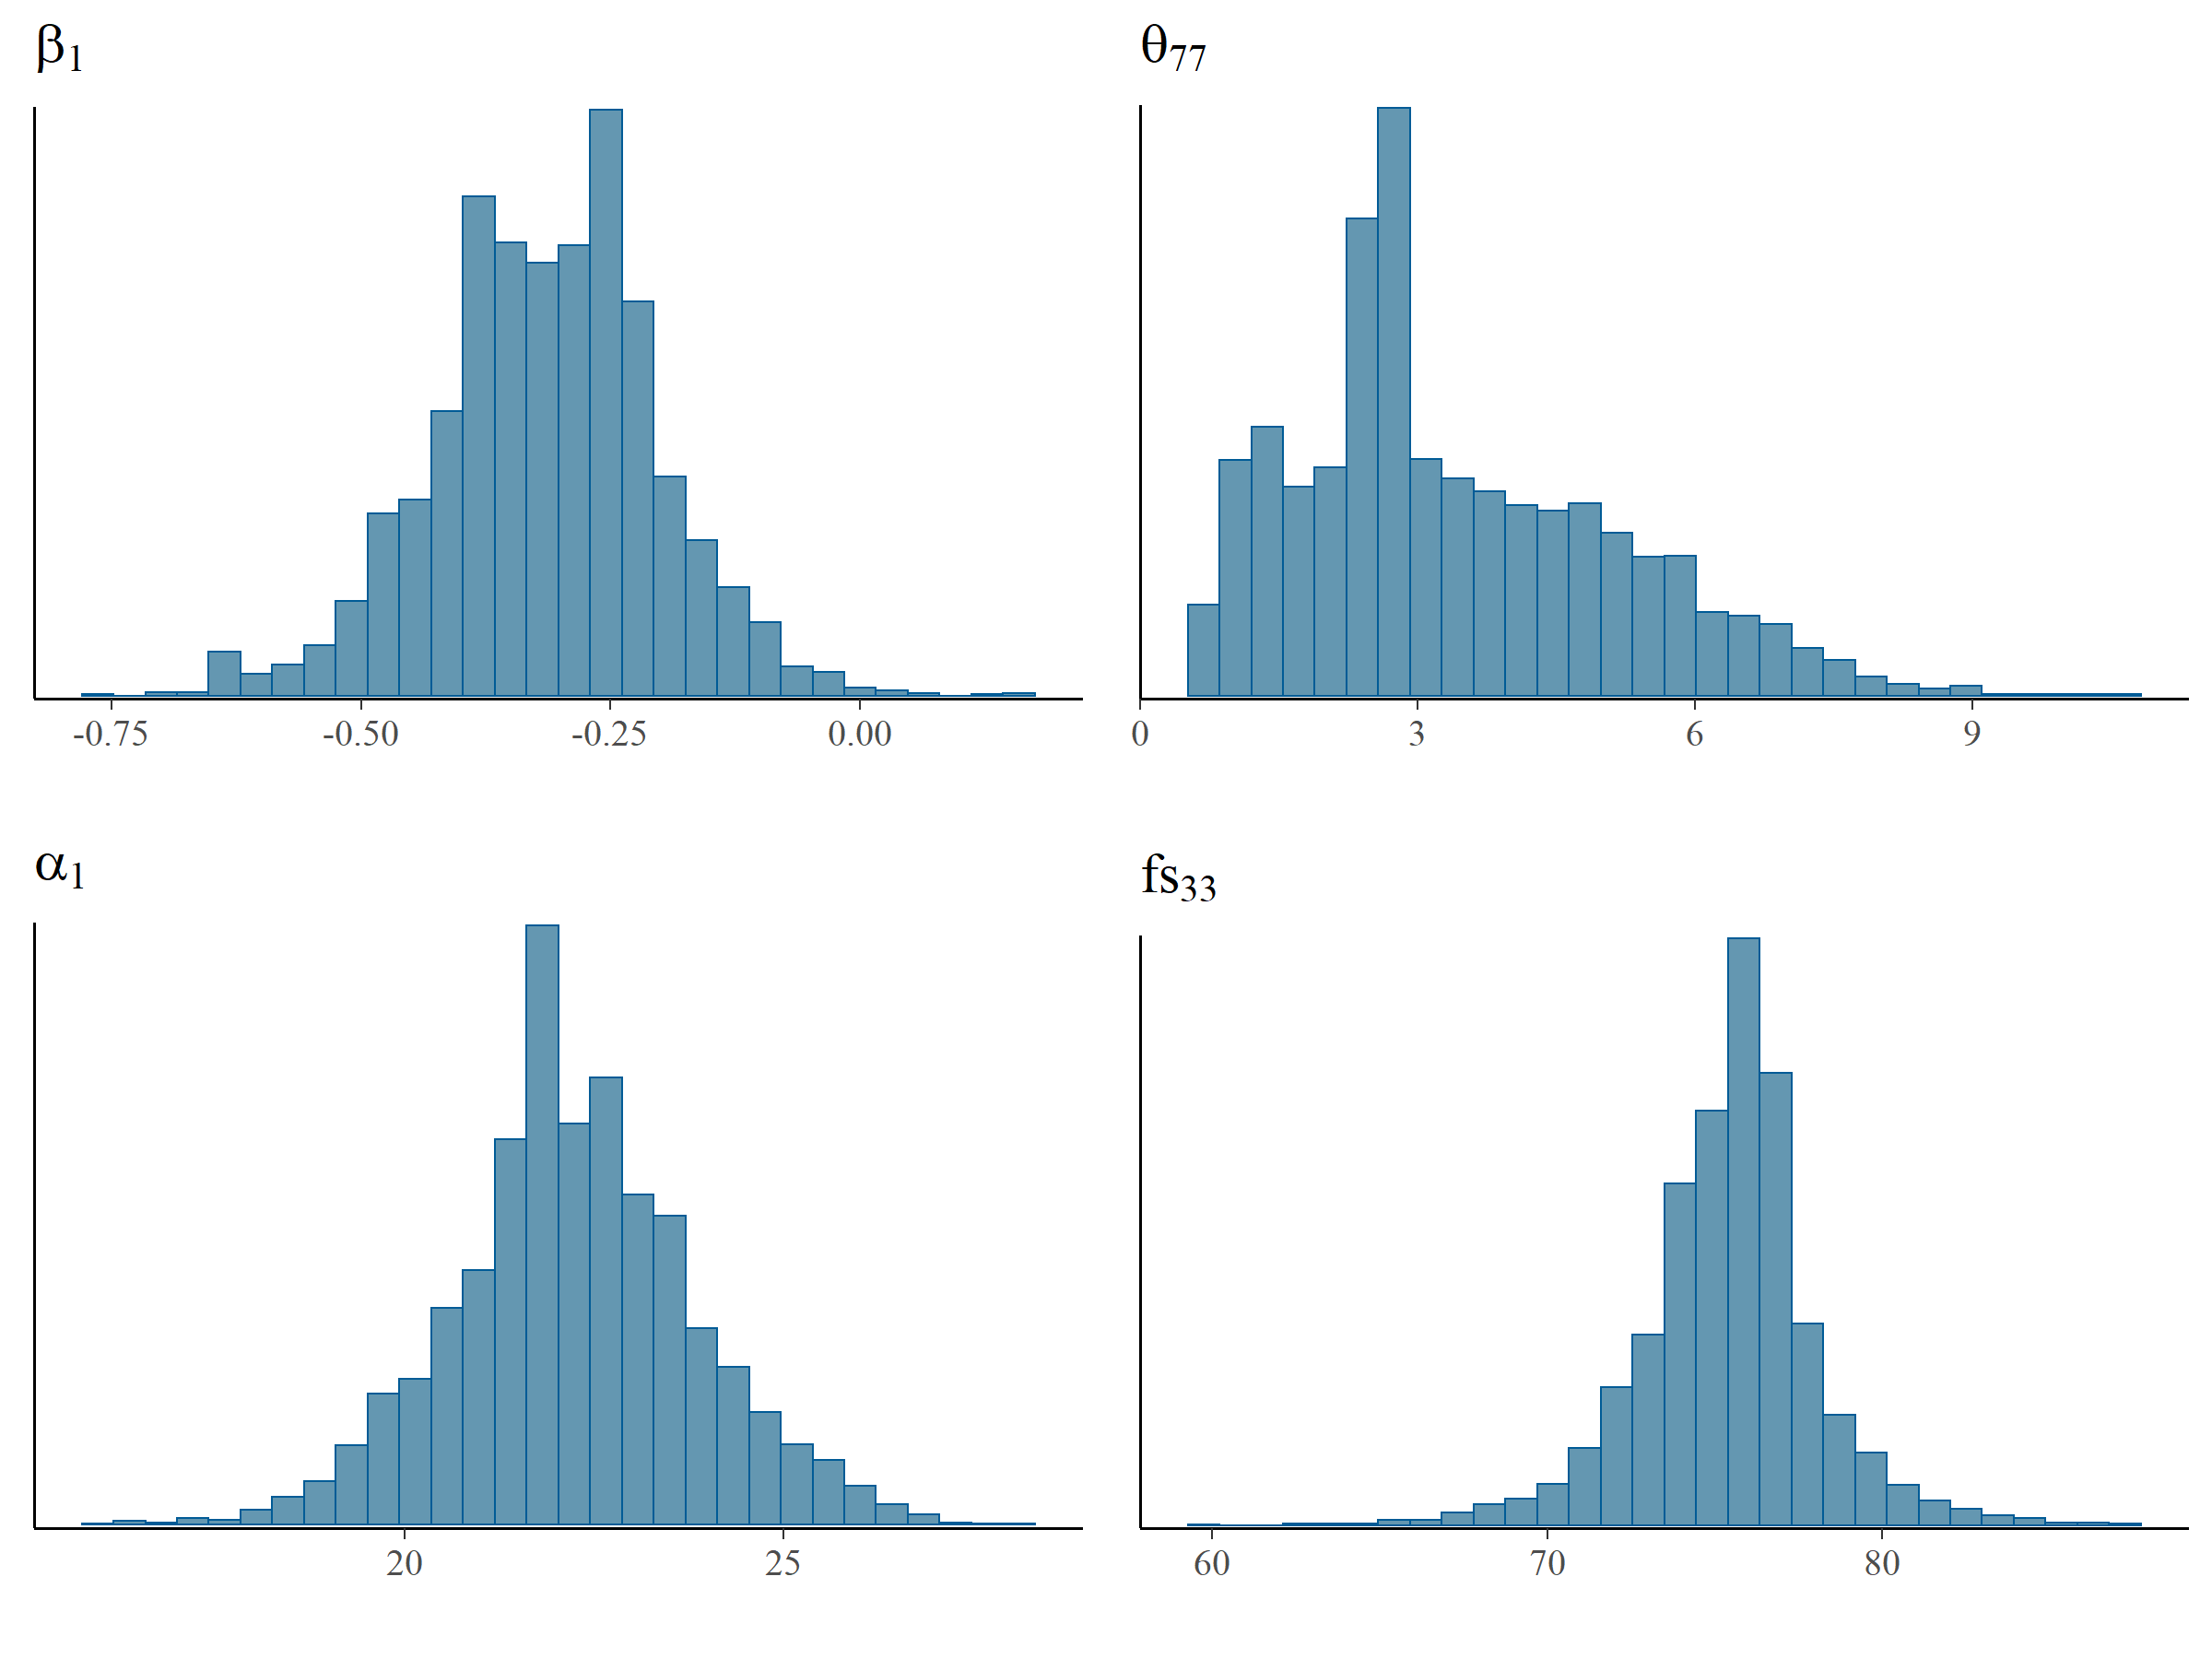
\includegraphics[width=0.7\linewidth]{figures/chapter_5/Figure4} 

}

\caption{Histograms of MCMC samples for $\alpha_1, \beta_1, \theta_{77}$ and $fs_{33}$. $\theta_{77}$ has a non-smooth histogram, which indicates low ESS while the smooth histogram for $fs_{33}$ is indicative of higher ESS.}\label{fig:ch05fig4}
\end{figure}

\newpage

\begin{figure}[H]

{\centering 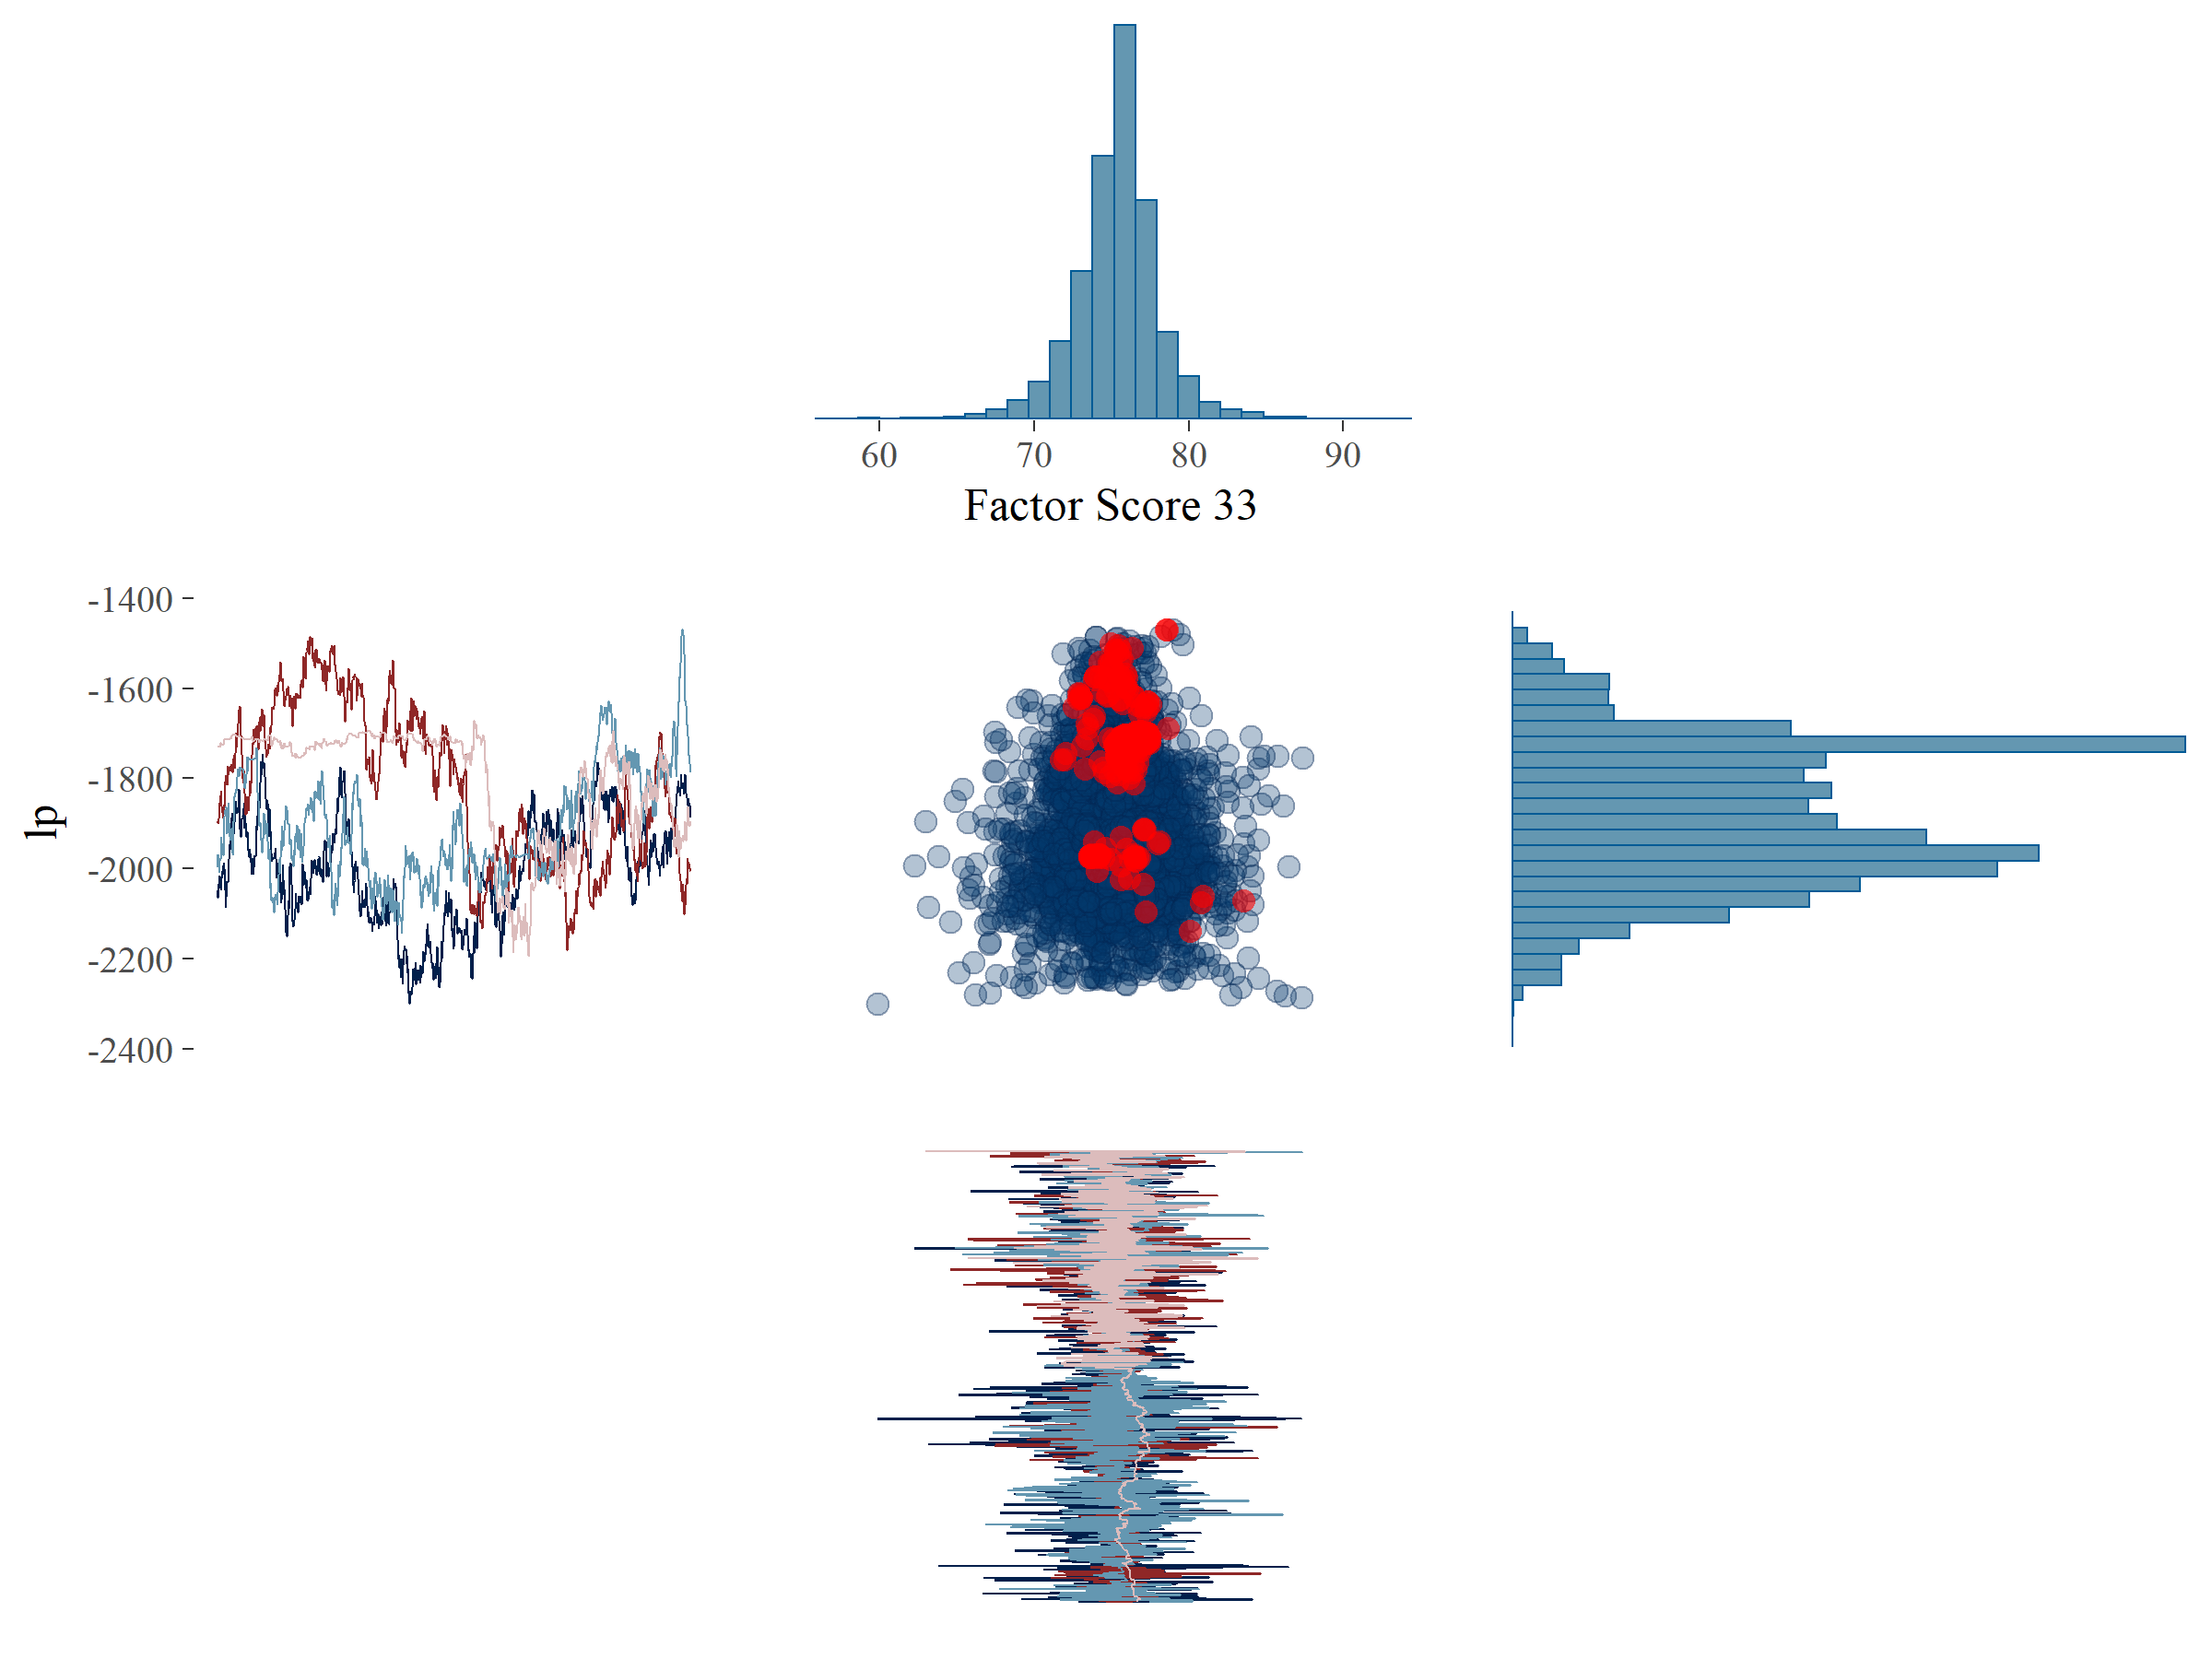
\includegraphics[width=0.9\linewidth]{C:/Users/Administrator/Dropbox/Werk/PhD UU/Dissertation/figures/chapter_5/Figure5/Figure5a} 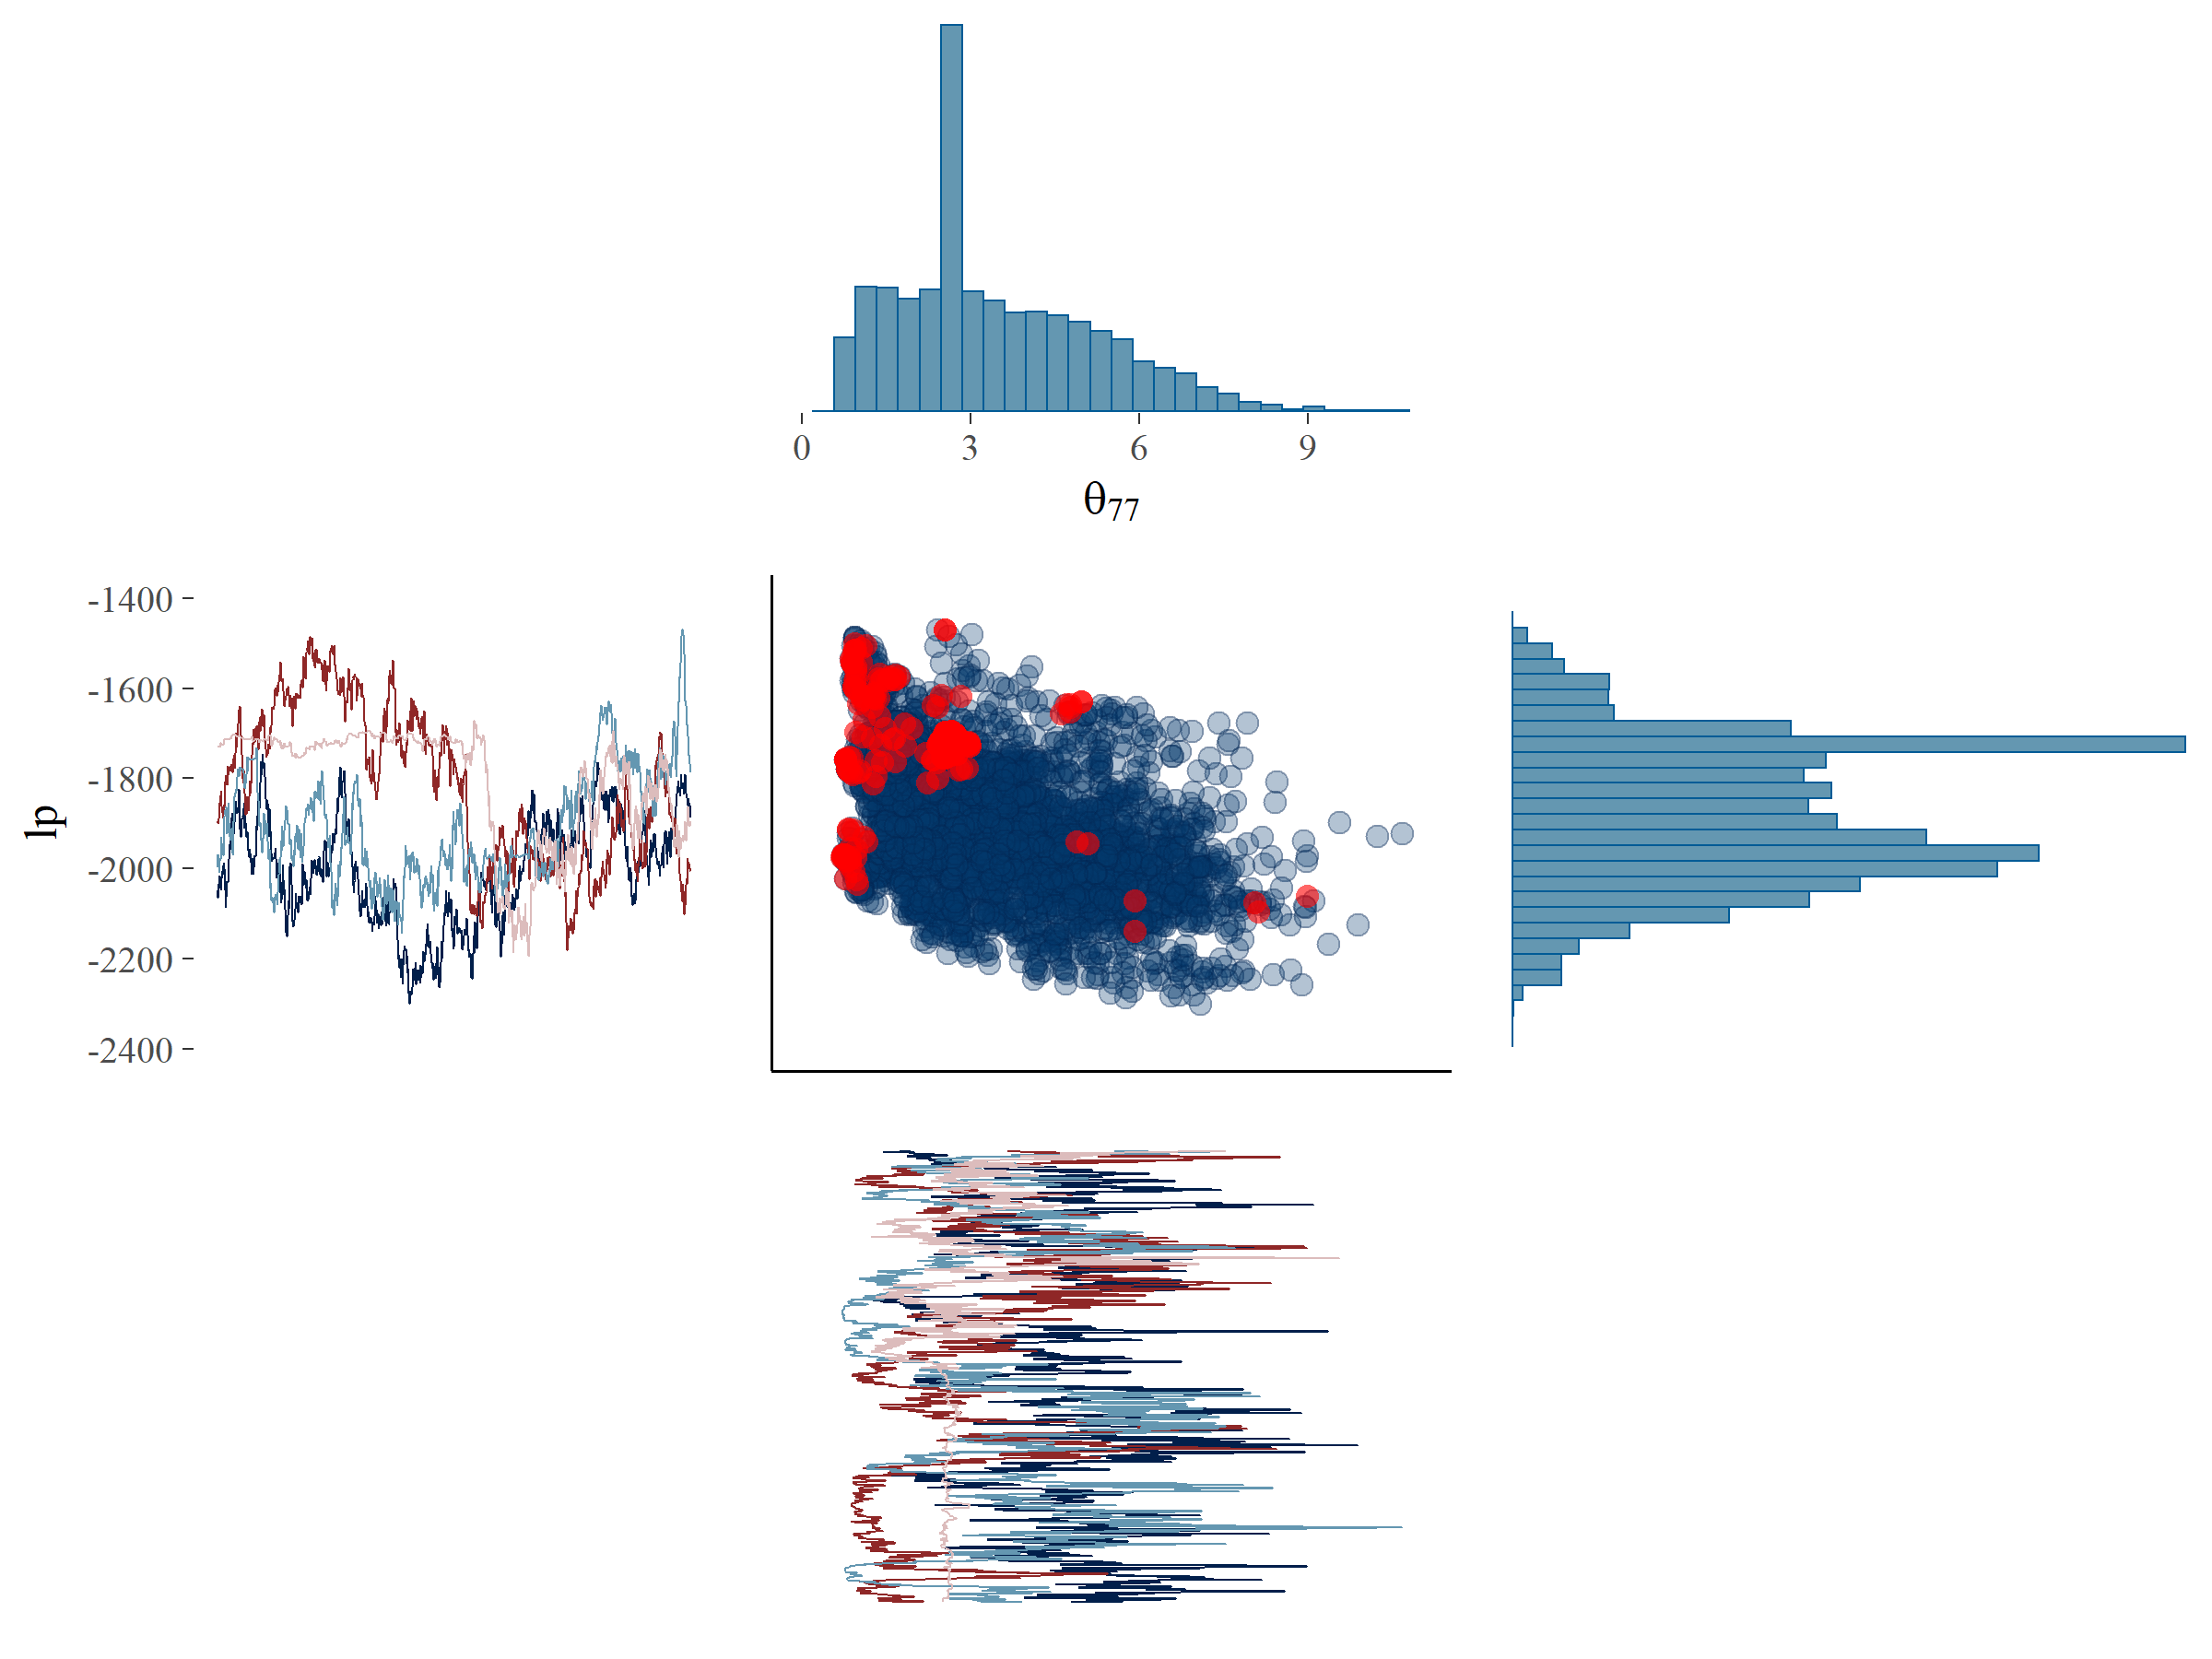
\includegraphics[width=0.9\linewidth]{C:/Users/Administrator/Dropbox/Werk/PhD UU/Dissertation/figures/chapter_5/Figure5/Figure5b} 

}

\caption{Plot of the posterior samples of $lp$ (y-axis) against $fs_{33}$ (x-axis, panel A) and $\theta_{77}$ (x-axis, panel B) with divergent transitions marked by red dots. Additionally, the histograms and trace plots of the corresponding parameters have been placed on the margins.}\label{fig:ch05fig5}
\end{figure}

\begin{figure}

{\centering 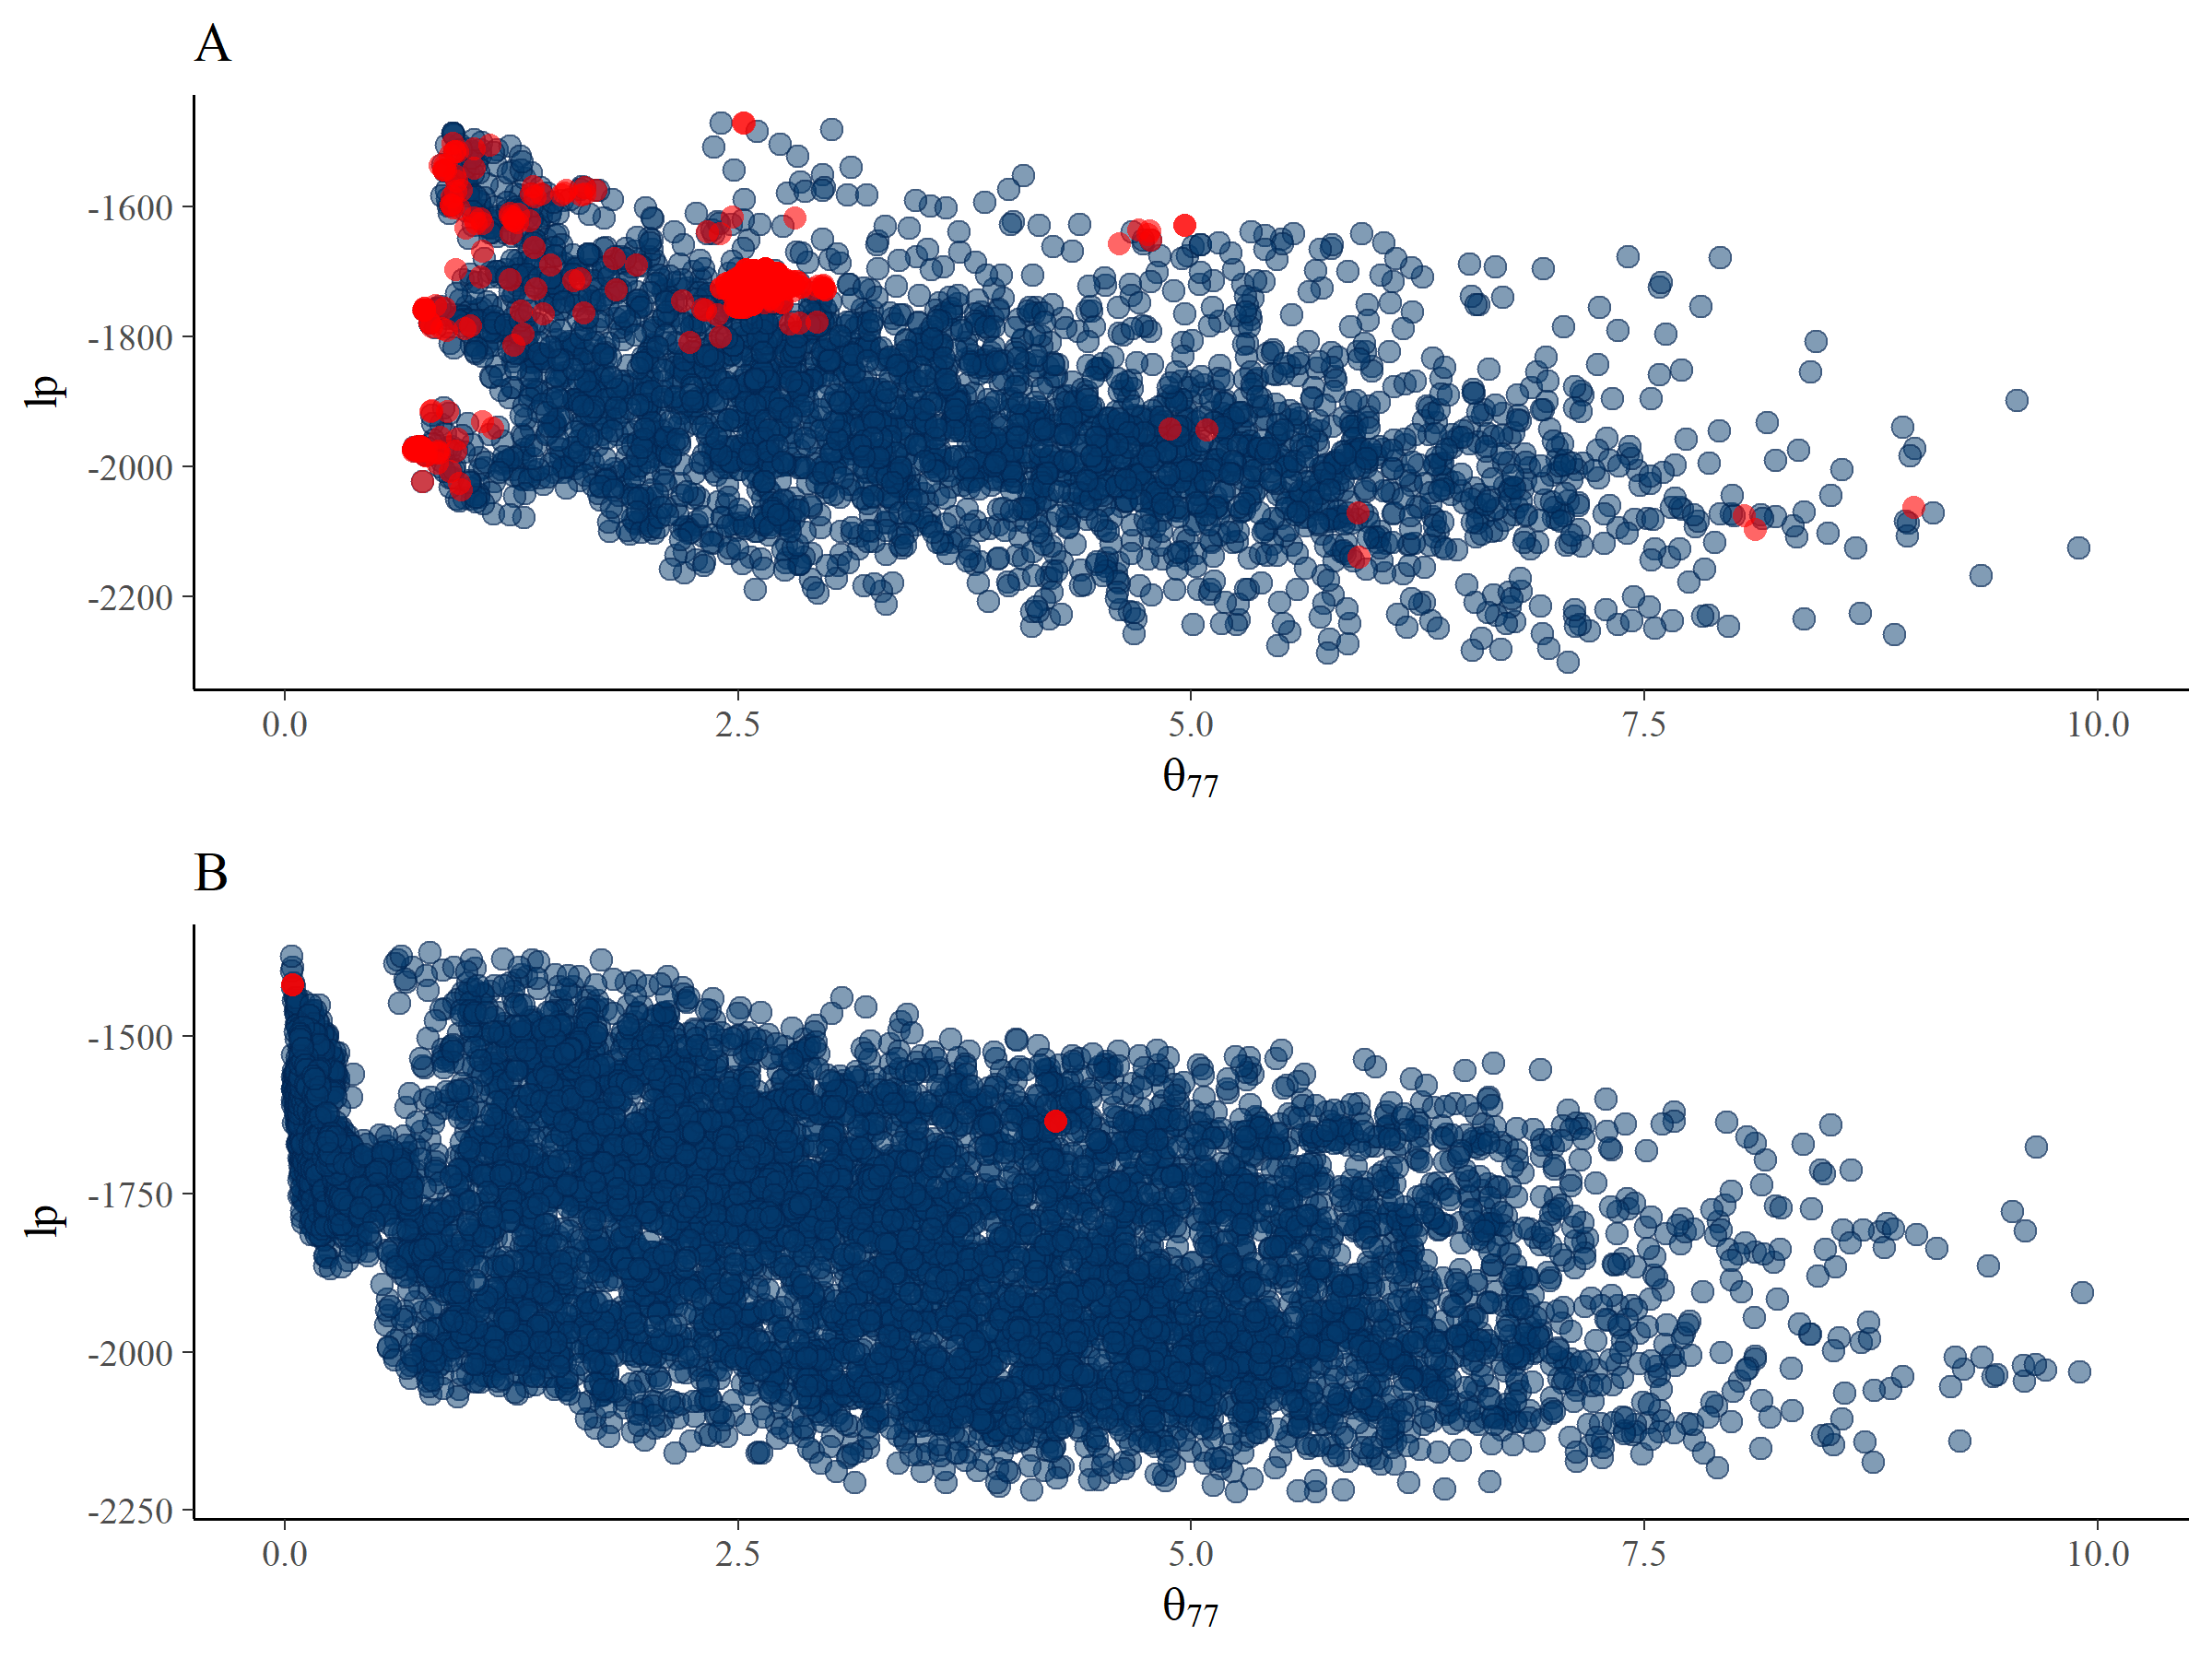
\includegraphics[width=0.8\linewidth]{figures/chapter_5/Figure6} 

}

\caption{Plots of the posterior samples of $lp$ against $\theta_{77}$ for the default estimation settings (panel A) and the estimation settings that have been forced to take smaller step sizes (panel B). Divergent transitions are indicated by red dots. }\label{fig:ch05fig6}
\end{figure}

\hypertarget{moving-forward-alternative-models}{%
\section{Moving forward: Alternative Models}\label{moving-forward-alternative-models}}

At this stage in the analysis process we continue to face difficulties with obtaining trustworthy posterior estimates due to divergent transitions. After exploring a smaller step size in the previous section, there are multiple options that can be considered and these can be based on statistical arguments, substantive theoretical arguments or, ideally, on both. Some statistical options can be sought in terms of the reparameterization of the model (Gelman, \protect\hyperlink{ref-gelman_parameterization_2004}{2004}), that is, the reformulation of the same model in an alternative form, for instance by using non-centered parametrizations in hierarchical models (Betancourt \& Girolami, \protect\hyperlink{ref-betancourt_hamiltonian_2015}{2015}). This needs to be done carefully and with consideration of the effects on prior implications and posterior estimates. The optimal course of action will differ from one situation to another, and we show five arbitrary ways of moving forward, but all require adjustments to the original analysis plan. We considered the following options:
1. Subgroup removal: We removed 32 cases that scored perfectly, i.e.~a score of 100, on the manifest variable \(x7\). This would potentially solve issues with the residual variance of \(x7\) (\(\theta_{77}\)).
2. Changing one of the priors: We specified a different prior on \(\theta_{77}\), namely, an Inverse Gamma (\(IG(0.5,0.5)\)) instead of a Half-Normal (\(HN(0,100)\)) (see: Van De Schoot et al., \protect\hyperlink{ref-van_de_schoot_analyzing_2015}{2015}). The IG prior forced the posterior distribution away from zero. If \(\theta_{77}\) was zero, this implies that \(x7\) is a perfect indicator of the latent variable. Since a perfect indicator is unlikely, we specified a prior that excludes this possibility.
3. Changing the distal outcome: We replaced the latent distal outcome with the manifest variable \(x7\). \(\theta_{77}\) estimates contained values of zero, which would indicate that x7 is a good or perfect indicator and could serve as a proxy for the latent variable. Replacing the latent factor with a single manifest indicator reduces the complexity of the model.
4. A possible increase of variance in the distal latent factor score: we removed cases that exhibited little variation between the scores on \(x6\) and \(x7\).

We ran the model using these four adjustments (see the OSF webpage for details). Table \ref{tab:ch05tab3} presents the posterior results of these additional analyses and an assessment of the extent to which the alternatives required adjustments to the original research question. The first three alternative solutions still contained divergent transitions and consequently the results could not be trusted. The fourth alternative solution did not result in divergent transitions. The ESS of the fourth alternative solution was still low, both in terms of the percentage of iterations and in absolute value (see Table \ref{tab:ch05tab2}). Although the low ESS in terms of percentage may not be resolved, the absolute ESS can be raised by increasing the total number of iterations. Even though we could draw conclusions using results from the fourth alternative solution, the rather arbitrary removal of cases changed the original research question. We investigated, and thus generalized to, a different population compared to the original analysis plan. Using an alternative model or a subset of the data could provide a solution to estimation issues. However, this could impact our substantive conclusions, e.g., see \(\beta_1\) in Table \ref{tab:ch05tab3}, for which the 95\% credibility interval in the fourth alternative contained zero, in contrast to credibility intervals for this parameter obtained using other alternative solutions. As substantive conclusions can be impacted by the choices we make, the transparency of the research process is crucial.

\blandscape

\footnotesize

\begin{longtable}[]{@{}ccccccc@{}}
\caption{\label{tab:ch05tab3} Results for the parameters of interest in the different models that we estimated. The mean parameter values are reported with the 95\% credibility intervals in brackets. The extent to which we need to adjust analytic strategy is assessed by the authors, DV for statistical input, and ME as the content specialist on this research area. Note that alternative III changes the actual model such that Figure \ref{fig:ch05fig1} is not an accurate representation anymore.}\tabularnewline
\toprule
\begin{minipage}[b]{0.11\columnwidth}\centering
Parameter\strut
\end{minipage} & \begin{minipage}[b]{0.12\columnwidth}\centering
Model with default
estimation settings\strut
\end{minipage} & \begin{minipage}[b]{0.13\columnwidth}\centering
Model with small
step size in
estimation setting\strut
\end{minipage} & \begin{minipage}[b]{0.11\columnwidth}\centering
Alternative I:
Remove perfect
HRQL scores\strut
\end{minipage} & \begin{minipage}[b]{0.11\columnwidth}\centering
Alternative II:
\(IG(0.5, 0.5)\)
prior for
\(\theta_{77}\)\strut
\end{minipage} & \begin{minipage}[b]{0.11\columnwidth}\centering
Alternative III:
Replace factor
score with \(x7\)\strut
\end{minipage} & \begin{minipage}[b]{0.12\columnwidth}\centering
Alternative IV:
Possible increase
of variance in
latent factor\strut
\end{minipage}\tabularnewline
\midrule
\endfirsthead
\toprule
\begin{minipage}[b]{0.11\columnwidth}\centering
Parameter\strut
\end{minipage} & \begin{minipage}[b]{0.12\columnwidth}\centering
Model with default
estimation settings\strut
\end{minipage} & \begin{minipage}[b]{0.13\columnwidth}\centering
Model with small
step size in
estimation setting\strut
\end{minipage} & \begin{minipage}[b]{0.11\columnwidth}\centering
Alternative I:
Remove perfect
HRQL scores\strut
\end{minipage} & \begin{minipage}[b]{0.11\columnwidth}\centering
Alternative II:
\(IG(0.5, 0.5)\)
prior for
\(\theta_{77}\)\strut
\end{minipage} & \begin{minipage}[b]{0.11\columnwidth}\centering
Alternative III:
Replace factor
score with \(x7\)\strut
\end{minipage} & \begin{minipage}[b]{0.12\columnwidth}\centering
Alternative IV:
Possible increase
of variance in
latent factor\strut
\end{minipage}\tabularnewline
\midrule
\endhead
\begin{minipage}[t]{0.11\columnwidth}\centering
\(\beta_0\)\strut
\end{minipage} & \begin{minipage}[t]{0.12\columnwidth}\centering
66.28
{[}39.58, 83.68{]}\strut
\end{minipage} & \begin{minipage}[t]{0.13\columnwidth}\centering
66.83
{[}38.89, 84.12{]}\strut
\end{minipage} & \begin{minipage}[t]{0.11\columnwidth}\centering
65.56
{[}48,78, 75.83{]}\strut
\end{minipage} & \begin{minipage}[t]{0.11\columnwidth}\centering
62.10
{[}30.95, 83.52{]}\strut
\end{minipage} & \begin{minipage}[t]{0.11\columnwidth}\centering
69.76
{[}39.04, 93.51{]}\strut
\end{minipage} & \begin{minipage}[t]{0.12\columnwidth}\centering
64.46
{[}47.21, 78.71{]}\strut
\end{minipage}\tabularnewline
\begin{minipage}[t]{0.11\columnwidth}\centering
\(\beta_1\)\strut
\end{minipage} & \begin{minipage}[t]{0.12\columnwidth}\centering
-0.32
{[}-0.55, -0.10{]}\strut
\end{minipage} & \begin{minipage}[t]{0.13\columnwidth}\centering
-0.31
{[}-0.53, -0.09{]}\strut
\end{minipage} & \begin{minipage}[t]{0.11\columnwidth}\centering
-0.23
{[}-0.44, -0.01{]}\strut
\end{minipage} & \begin{minipage}[t]{0.11\columnwidth}\centering
-0.32
{[}-0.53, -0.10{]}\strut
\end{minipage} & \begin{minipage}[t]{0.11\columnwidth}\centering
-0.40
{[}-0.67, -0.11{]}\strut
\end{minipage} & \begin{minipage}[t]{0.12\columnwidth}\centering
-0.22
{[}-0.51, 0.10{]}\strut
\end{minipage}\tabularnewline
\begin{minipage}[t]{0.11\columnwidth}\centering
\(\beta_2\)\strut
\end{minipage} & \begin{minipage}[t]{0.12\columnwidth}\centering
-31.87
{[}-74.80, -7.63{]}\strut
\end{minipage} & \begin{minipage}[t]{0.13\columnwidth}\centering
-31.46
{[}-76.41, -7.42{]}\strut
\end{minipage} & \begin{minipage}[t]{0.11\columnwidth}\centering
-19.39
{[}-44.93, -7.47{]}\strut
\end{minipage} & \begin{minipage}[t]{0.11\columnwidth}\centering
-39.16
{[}-92,18,-7.81\strut
\end{minipage} & \begin{minipage}[t]{0.11\columnwidth}\centering
-47.06
{]} {[}-96.94, -12\strut
\end{minipage} & \begin{minipage}[t]{0.12\columnwidth}\centering
-35.66
.19{]} {[}-64.16, -15.30{]}\strut
\end{minipage}\tabularnewline
\begin{minipage}[t]{0.11\columnwidth}\centering
\(\beta_3\)\strut
\end{minipage} & \begin{minipage}[t]{0.12\columnwidth}\centering
-0.61
{[}-0.92, -0.31{]}\strut
\end{minipage} & \begin{minipage}[t]{0.13\columnwidth}\centering
-0.62
{[}-0.93, -0.31{]}\strut
\end{minipage} & \begin{minipage}[t]{0.11\columnwidth}\centering
-0.40
{[}-0.67, -0.14{]}\strut
\end{minipage} & \begin{minipage}[t]{0.11\columnwidth}\centering
-0,61
{[}-0,93, -0,30{]}\strut
\end{minipage} & \begin{minipage}[t]{0.11\columnwidth}\centering
-0.78
{[}-1.16, -0.41{]}\strut
\end{minipage} & \begin{minipage}[t]{0.12\columnwidth}\centering
-0.53
{[}-1.02, -0.06{]}\strut
\end{minipage}\tabularnewline
\begin{minipage}[t]{0.11\columnwidth}\centering
\(\sigma_\epsilon\)\strut
\end{minipage} & \begin{minipage}[t]{0.12\columnwidth}\centering
8.36
{[}3.77, 10.88{]}\strut
\end{minipage} & \begin{minipage}[t]{0.13\columnwidth}\centering
7.93
{[}2.92, 10.77{]}\strut
\end{minipage} & \begin{minipage}[t]{0.11\columnwidth}\centering
4.76
{[}0.54, 8.29{]}\strut
\end{minipage} & \begin{minipage}[t]{0.11\columnwidth}\centering
7.40
{[}1.98, 10.87{]}\strut
\end{minipage} & \begin{minipage}[t]{0.11\columnwidth}\centering
10.06
{[}3.73, 13.74{]}\strut
\end{minipage} & \begin{minipage}[t]{0.12\columnwidth}\centering
6.63
{[}2.07, 10.63{]}\strut
\end{minipage}\tabularnewline
\begin{minipage}[t]{0.11\columnwidth}\centering
Divergent
transitions
present\strut
\end{minipage} & \begin{minipage}[t]{0.12\columnwidth}\centering
YES\strut
\end{minipage} & \begin{minipage}[t]{0.13\columnwidth}\centering
YES\strut
\end{minipage} & \begin{minipage}[t]{0.11\columnwidth}\centering
YES\strut
\end{minipage} & \begin{minipage}[t]{0.11\columnwidth}\centering
YES\strut
\end{minipage} & \begin{minipage}[t]{0.11\columnwidth}\centering
YES\strut
\end{minipage} & \begin{minipage}[t]{0.12\columnwidth}\centering
NO\strut
\end{minipage}\tabularnewline
\begin{minipage}[t]{0.11\columnwidth}\centering
To what extent
do we need to
adjust analytic
strategy?\strut
\end{minipage} & \begin{minipage}[t]{0.12\columnwidth}\centering
Not at all\strut
\end{minipage} & \begin{minipage}[t]{0.13\columnwidth}\centering
Not at all\strut
\end{minipage} & \begin{minipage}[t]{0.11\columnwidth}\centering
Substantially;
we generalize
to a different
(known)
population.\strut
\end{minipage} & \begin{minipage}[t]{0.11\columnwidth}\centering
Negligible;
theory behind
research
question
remains the
same.\strut
\end{minipage} & \begin{minipage}[t]{0.11\columnwidth}\centering
Substantially;
data-driven
change of model
(replacing
measurement model
with a single
manifest
variable).\strut
\end{minipage} & \begin{minipage}[t]{0.12\columnwidth}\centering
Substantially;
we generalize
to a different
(unknown)
population.\strut
\end{minipage}\tabularnewline
\bottomrule
\end{longtable}

\elandscape

\hypertarget{conclusion}{%
\section{Conclusion}\label{conclusion}}

Bayesian estimation with (weakly) informative priors is suggested as a solution to deal with small sample size issues. The current chapter illustrated the process of conducting Bayesian estimation with (weakly) informative priors along with the potential problems that can arise. The WAMBS-checklist was a helpful tool in this process, and we propose supplementing the checklist steps with an inspection of the effective number of samples taken using MCMC. As we have shown, a low ESS can point toward specific parameters to investigate, which is especially useful for complex models with many parameters, as investigating each parameter individually would be time-consuming. We recommend using advanced statistical software (such as stan) because the implemented algorithms (e.g., HMC or NUTS) can have a positive impact on the ESS, and estimates of ESS are readily available. Moreover, the use of advanced algorithms such as HMC or NUTS provides additional diagnostic information about the estimation in the form of divergent transitions, which can be used in addition to the WAMBS-checklist.

The empirical example showed that even Bayesian estimation with informative priors has limits in terms of its performance for complex models with small sample sizes. Thus, using a Bayesian analysis should not be considered a `quick fix'. Careful consideration of the analysis steps and the intermediate results is imperative. Different solutions can differentially impact the posterior parameter estimates and thereby the substantive conclusions, and there is a need for constant interaction and collaboration between applied researchers, who formulate the research questions, and the statisticians, who possess the statistical and methodological knowledge.

\hypertarget{acknowledgements}{%
\section{Acknowledgements}\label{acknowledgements}}

Both authors were supported by the Netherlands Organization for Scientific Research (grant number NWO-VIDI-452-14-006). This work was a result of the collaborative efforts of our project team, including Dr.~Nancy van Loey and prof. Dr.~Rens van de Schoot. The synthetic data used in the empirical example were based on a study funded by the Dutch Burns Foundation (Grant No.~07.107). We thank all participating parents and the research team in the burn centers in the Netherlands and Belgium.

\hypertarget{elicitlgm}{%
\chapter{Expert Elicitation in the Social Sciences: The case of Posttraumatic Stress Symptoms Development in Children with Burn Injuries}\label{elicitlgm}}

\chaptermark{ELICITATION IN THE SOCIAL SCIENCES}
\thispagestyle{empty}

\blfootnote{This chapter is submitted for publication as Veen, D., Egberts, M. R., Van Loey, N. E. E. \& Van de Schoot, R. \textit{Expert Elicitation in the Social Sciences: The case of Posttraumatic Stress Symptoms Development in Children with Burn Injuries} \\
\indent All authors have been involved in the design of the study and the elicitation procedure. DV programmed the elicitation software. ME arranged the elicitation meetings with the experts. DV and ME conducted all elicitation procedures together. DV wrote and revised the paper with contributions and feedback provided by ME, NvL and RvdS.}

\hypertarget{abstract-4}{%
\section*{Abstract}\label{abstract-4}}
\addcontentsline{toc}{section}{Abstract}

\small

Experts provide an alternative source of information to classical data collection methods such as surveys. They can provide additional insight into problems, supplement existing data or provide insights when classical data collection is troublesome. In this paper we explore the (dis)similarities between expert judgements and data collected by traditional data collection methods regarding the development of Posttraumatic Stress Symptoms (PTSS) in children with burn injuries. By means of an elicitation procedure the experts' domain expertise are formalized and represented in the form of probability distributions. The method is used to obtain beliefs from 14 experts, including nurses and psychologists, and those beliefs are contrasted with questionnaire data collected by Egberts, Van de Schoot, Geenen, \& Van Loey (\protect\hyperlink{ref-egberts_mother_2018}{2018}) on the same issue. The individual and aggregated expert judgements are contrasted with the questionnaire data by means of Kullback-Leibler divergences. The aggregated judgements of the group that mainly includes psychologists resembles the questionnaire data more than almost all individual experts.

\normalsize
\newpage

\hypertarget{ch06introduction}{%
\section{Introduction}\label{ch06introduction}}

Expert elicitation entails the extraction of information from experts and the translation of this information into a probabilistic representation and there are many reasons to elicit expert knowledge. For instance to supplement existing data using priors that are informed by expert knowledge (Schoot, Sijbrandij, et al., \protect\hyperlink{ref-van_de_schoot_bayesian_2018}{2018}). Alternatively, some data have information gaps that can be filled by means of expert judgements (Dodd, Yuen, Sismanidis, Seddon, \& Jenkins, \protect\hyperlink{ref-dodd_global_2017}{2017}; Fischer et al., \protect\hyperlink{ref-fischer_estimating_2013}{2013}) or when data are present expert judgements can serve as a quality control for the data (Veen, Stoel, Schalken, Mulder, \& Schoot, \protect\hyperlink{ref-veen_using_2018}{2018}). Elicitation can also be used for forecasting purposes (Murphy \& Winkler, \protect\hyperlink{ref-murphy_subjective_1974}{1974}, \protect\hyperlink{ref-murphy_probability_1984}{1984}) or when there is no data available at all (Hald et al., \protect\hyperlink{ref-hald_world_2016}{2016}; Ho \& Smith, \protect\hyperlink{ref-ho_volcanic_1997}{1997}). The use of expert knowledge is widespread across many disciplines. To give some examples, Dodd et al. (\protect\hyperlink{ref-dodd_global_2017}{2017}) elicited expert based estimates for case-fatality ratios in HIV-positive children with tuberculosis who did not receive treatment. Barons et al. (\protect\hyperlink{ref-barons_eliciting_2018}{2018}) describe the use of expert judgements to create decision support systems with an example in food security and Dewispelare, Herren, \& Clemen (\protect\hyperlink{ref-dewispelare_use_1995}{1995}) describe expert elicitation in relation to the long-term behavior of high-level nuclear waste repositories. For numerous other examples on elicitation practices see for instance Chapter 10 of O'Hagan et al. (\protect\hyperlink{ref-ohagan_uncertain_2006}{2006}) listing applications in sales, medicine, nuclear industry, veterinary science and many more. Alternatively, examples using a specific elicitation tool are given in Gosling (\protect\hyperlink{ref-gosling_shelf:_2018}{2018}), or see Cooke \& Goossens (\protect\hyperlink{ref-cooke_tu_2008}{2008}) who describe a data base of over 67,000 elicited judgements.

Recently, there is a growing interest in the use of expert elicitation in the social sciences. Where Van de Schoot et al. (\protect\hyperlink{ref-van_de_schoot_systematic_2017}{2017}) only found two cases that reported the use of expert opinions to inform priors in 25 years of Bayesian statistics in psychology, this trend might slowly be changing. Gronau, Ly, \& Wagenmakers (\protect\hyperlink{ref-gronau_informed_2019}{2019}) elicited expert judgements on effects sizes such that these could be used in informed Bayesian t-tests, in their example related to a replication study in the field of psychology. Lek \& Van de Schoot (\protect\hyperlink{ref-lek_development_2018}{2018}) elicited prior distribution from teachers concerning the math abilities of their students. Zondervan-Zwijnenburg et al. (\protect\hyperlink{ref-zondervan-zwijnenburg_application_2017}{2017}\protect\hyperlink{ref-zondervan-zwijnenburg_application_2017}{b}) elicited expert judgements on the correlation between cognitive potential and academic performance. Moreover, methods are being developed to facilitate expert elicitation in a flexible manner such that experts are guided in the elicitation process (Veen et al., \protect\hyperlink{ref-veen_proposal_2017}{2017}).

Whatever the reasons of the elicitation, the goal is to get an accurate representation of the experts' beliefs and associated (un)certainty and enable the representation of the experts' domain knowledge in terms of a probability distribution. Overconfidence of experts is one of the crucial issues in expert elicitation (O'Hagan et al., \protect\hyperlink{ref-ohagan_uncertain_2006}{2006}), resulting in elicited probability distributions with little uncertainty. In the seminal work of O'Hagan et al. (\protect\hyperlink{ref-ohagan_uncertain_2006}{2006}) feedback is named as the most natural way to improve the accuracy of elicited beliefs and interactive software as almost essential for the effective use of feedback. This is corroborated by Goldstein \& Rothschild (\protect\hyperlink{ref-goldstein_lay_2014}{2014}) who found that visual feedback can increase even laypeople's intuitions about probability distributions. Over a decade has passed since the advice by O'Hagan et al. (\protect\hyperlink{ref-ohagan_uncertain_2006}{2006}) and many have followed the advice. Elicitation software can be split into more general and more custom variations. Some more general frameworks are, for instance, ElicitN which was developed by Fisher et al. (\protect\hyperlink{ref-fisher_software_2012}{2012}) for the elicitation of count data. Truong, Heuvelink, \& Gosling (\protect\hyperlink{ref-truong_web-based_2013}{2013}) made a web-based tool for the elicitation of variogram estimates which describe a degree of spacial dependence. The elicitator was developed for indirect elicitation, creating a scenario based elicitation (James, Choy, \& Mengersen, \protect\hyperlink{ref-james_elicitator:_2010}{2010}; Low-Choy, James, Murray, \& Mengersen, \protect\hyperlink{ref-low-choy_elicitator:_2012}{2012}). Morris et al. (\protect\hyperlink{ref-morris_web-based_2014}{2014}) developed MATCH which is based on the R package SHELF (Oakley, \protect\hyperlink{ref-R-SHELF}{2019}) and which is a very general elicitation tool that allows multiple elicitation methods to be used interactively to elicit single parameters. Garthwaite, Al-Awadhi, Elfadaly, \& Jenkinson (\protect\hyperlink{ref-garthwaite_prior_2013}{2013}) developed an elicitation procedure for generalized linear and piecewise-linear models, Runge, Scherbaum, Curtis, \& Riggelsen (\protect\hyperlink{ref-runge_interactive_2013}{2013}) for seismic-hazard analysis and Elfadaly \& Garthwaite (\protect\hyperlink{ref-elfadaly_eliciting_2017}{2017}) for eliciting Dirichlet and Gaussian copula prior distributions. Sometimes more customized software is developed for specific elicitation settings (e.g.~Bojke et al., \protect\hyperlink{ref-bojke_eliciting_2010}{2010}; Haakma, Steuten, Bojke, \& IJzerman, \protect\hyperlink{ref-haakma_belief_2014}{2014}; Hampson, Whitehead, Eleftheriou, \& Brogan, \protect\hyperlink{ref-hampson_bayesian_2014}{2014}; Hampson et al., \protect\hyperlink{ref-hampson_elicitation_2015}{2015}). The use of software, customized or not, to increase the accuracy of the elicited beliefs is now common practice.

In this paper we present an elicitation methodology especially designed for eliciting parameters of a Latent Growth Curve Model (LGM) regarding the development of Posttraumatic Stress Symptoms (PTSS) in children with burn injuries. LGMs are commonly used to analyze longitudinal data, especially in the social sciences (e.g.~Buist, Dekovic, Meeus, \& Van Aken, \protect\hyperlink{ref-buist_developmental_2002}{2002}; Catts, Bridges, Little, \& Tomblin, \protect\hyperlink{ref-catts_reading_2008}{2008}; Orth, Robins, \& Widaman, \protect\hyperlink{ref-orth_life-span_2012}{2012}). These models include repeated measurements of observed variables, and allow researchers to examine change or development over time in the construct of interest. For extensive explanations of LGMs see Duncan \& Duncan (\protect\hyperlink{ref-duncan_introduction_2004}{2004}), Little (\protect\hyperlink{ref-little_longitudinal_2013}{2013}), and Little, Bovaird, \& Slegers (\protect\hyperlink{ref-little_methods_2006}{2006}). Because the incidence of severe burn injuries in school-aged children and adolescents is relatively low, obtaining a sufficient sample to estimate LGMs is challenging. Nevertheless, to gain knowledge on the development of posttraumatic stress symptoms in this group of children, these types of models are favored over simpler models. Expert elicitation might provide and alternative, or supplement, to data collection for cases like our motivating example where traditional data is sparse.

The main aim of this paper is to compare domain expertise, expressed by experts in an elicitation setting, to data on the same topic collected by means of traditional data collection methods. Comparing experts' domain knowledge to traditional data collection methods can provide unique insights into the topic of interest and the perception thereof. In the remainder of this paper we first describe the methodology that is used to elicit the expert judgements. The methodology is an extension of the Five-Step Method (Veen et al., \protect\hyperlink{ref-veen_proposal_2017}{2017}), adapted to elicited multiple parameters. We elicit expert judgements from 14 experts, including nurses and psychologists. Thereafter, we compare individual expert judgements, aggregated group level expert judgements, and data collected by mean of traditional methods with one another and reflect on the elicitation procedure. Finally, we conclude the paper with a discussion section including recommendations for future research. All related materials for this study, including code and data, can be found on the Open Science Framework (OSF) webpage for this project at \url{https://osf.io/y5evf/}.

\hypertarget{methods}{%
\section{Methods}\label{methods}}

In the first section we describe the motivating example for this study. In the next section we elaborate on the elicitation procedure and software that has been developed. Finally, we describe the sample of experts (\(N=14\)) participating in the elicitation study. The study receive ethical approval from our internal Ethics Committee of the Faculty of Social and Behavioural Sciences of Utrecht University. The letter of approval can be found in the data archive on the \href{https://osf.io/y5evf/}{OSF website for this project}.

\hypertarget{motivating-example}{%
\subsection{Motivating Example}\label{motivating-example}}

The motivating example for this paper is the development of Posttraumatic Stress Symptoms (PTSS) in children after a burn event. In a prospective study on child and parent adjustment after pediatric burns, data on these symptoms were collected in three Dutch and four Belgian burn centers. Children aged 8-18 years old were eligible to participate in the study if they had been hospitalized for more than 24 hours and if the percentage total body surface area (TBSA) burned was at least 1\%. In Egberts et al. (\protect\hyperlink{ref-egberts_mother_2018}{2018}), a more detailed description of the overall study and sample can be found here. This sample consists of 100 children that reported on their symptoms of traumatic stress within the first month after the burn event (T1), and subsequently at 3 (T2) months post-burn. For the purpose of the current study, we also included the measures obtained 12 months (T3) post-burn. Children filled out the Children's Responses to Trauma Inventory (CRTI, revised version; Alisic, Eland, \& Kleber (\protect\hyperlink{ref-alisic_childrens_2006}{2006})). This measure assesses four symptom clusters of posttraumatic stress, including intrusion (e.g., repetitive, intrusive recollections of the trauma), avoidance (e.g., avoiding conversations of the event), arousal (e.g., difficulty concentrating), and other child-specific responses (e.g., feelings of guilt). Further details on this measure can be found in Alisic, Eland, Huijbregts, \& Kleber (\protect\hyperlink{ref-alisic_manual_2011}{2011}).

As the current study includes three measurements of PTSS at different time points a straightforward model to analyse the development of PTSS symptoms is an LGM. Figure \ref{fig:ch06fig1} provides a visual representation of an LGM for this motivating example. The model is parameterized such that the latent intercept provides an estimate for PTSS in the first month after the burn event. The latent slope describes the change in PTSS one year post-burn. Parameterizing the slope by year instead of per month is done to ease the reasoning in the elicitation procedure. Furthermore, the scale of the PTSS scores has been standardized for the data of the prospective study and for the elicitation study. The scores can fall between 0-100. A zero score means that none of the symptoms of any of the clusters of posttraumatic stress are present. A score of 100 means that all symptoms from all clusters are present to their maximum extent. A standardized cut-off value of 42 was used to indicate clinical relevance of symptoms and corresponds to the cut-off value provided in the CRTI manual.

\begin{figure}

{\centering 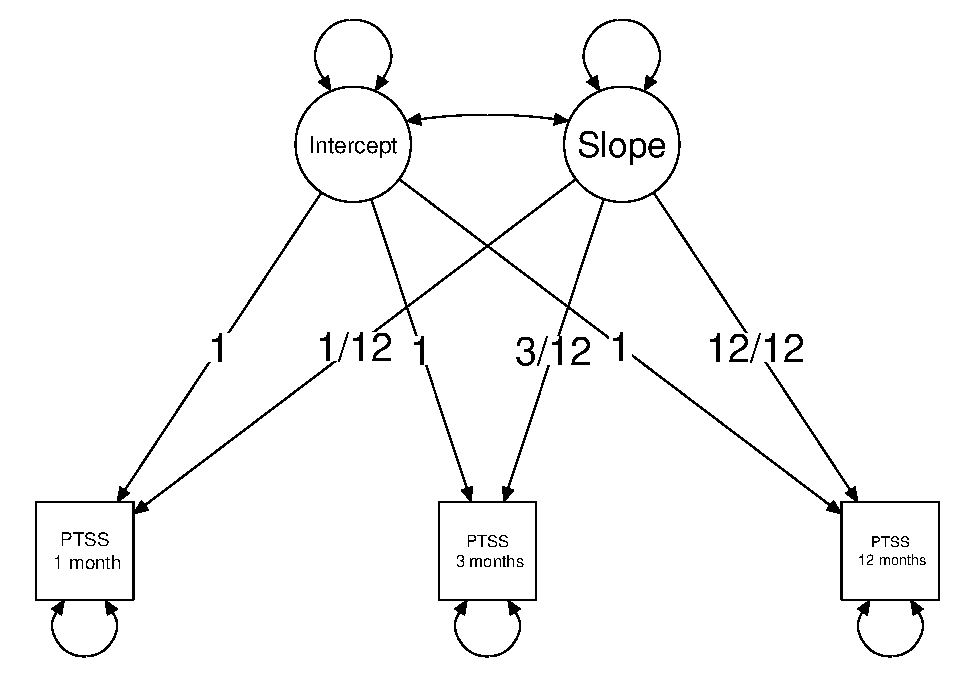
\includegraphics[width=0.5\linewidth]{Dissertation_Duco_Veen_files/figure-latex/ch06fig1-1} 

}

\caption{Visual representation of a Latent Growth Curve Model with three observed time points for PTSS. }\label{fig:ch06fig1}
\end{figure}

\hypertarget{expert-elicitation-1}{%
\subsection{Expert Elicitation}\label{expert-elicitation-1}}

To optimally prepare the experts within the limited time that was allocated for each elicitation a short introduction was presented by the researchers conducting the elicitation (DV \& ME), hereafter named the facilitators. The facilitators presented the experts with a brief overview of what expert elicitation is, what it can be used for and how to interpret the probability distributions that are used to represent their beliefs. Thereafter, to familiarize the experts with the elicitation procedure itself, an example elicitation for an unrelated topic was presented to the experts using the same elicitation tool. After the example elicitation the facilitators introduced the specifics related to the motivating example and the actual elicitation. The population, measurement scale, CRTI with the relevant symptom clusturs, and research question were introduced and experts were invited to ask questions to clarify any part of the procedure. Once the experts stated that they were ready to continue with the elicitation they were requested to sign the informed consent letter, which they received prior to the elicitation. If they agreed, they also agreed to the recording of the elicitation procedure. The experts were requested to reason aloud during the elicitation. The recordings were transcribed to provide additional insights in the elicitation procedure and possible differences between experts. The experts carried out the elicitation procedure using the software that is described next.

The software and procedure in this study was based on the Five-Step Method, developed by Veen et al. (\protect\hyperlink{ref-veen_proposal_2017}{2017}), with a slight adaptation to elicit multiple parameters instead of a single parameter. The Five-Step Method decomposes the elicitation process in multiple smaller steps, providing visual feedback at each stage of the elicitation procedure. By decomposing the elicitation task and providing visual feedback the procedures aims to reduce bias, for instance from overconfidence. The software has been developed in the form of a shiny web application (Chang et al., \protect\hyperlink{ref-R-shiny}{2019}). Using shiny to develop elicitation tools is not uncommon, see for instance Hampson et al. (\protect\hyperlink{ref-hampson_bayesian_2014}{2014}), Hampson et al. (\protect\hyperlink{ref-hampson_elicitation_2015}{2015}) and the original Five-Step Method by Veen et al. (\protect\hyperlink{ref-veen_proposal_2017}{2017}). In what follows we describe the Five-Step Method as implemented for this specific study, note that steps 3 and 4 were repeated for each parameter.

\textbf{Step 1.} Ten individual PTSS trajectories were elicited for an LGM. These individual trajectories should be representative for the population. From these individual trajectories we could deduce information on the point estimates for the average intercept and average slope parameters. This first step is called indirect elicitation because no statement is required directly concerning the parameters of interest. Figure \ref{fig:ch06fig2} provides a visual representation of step one.

\textbf{Step 2.} Feedback was provided on the average trajectory that was based upon the ten individual trajectories that the expert provided. The expert could accept this as the average trajectory, and thereby accept point estimate for the average intercept and slope, or the expert could adjust their input in step one. Figure \ref{fig:ch06fig3} provides a visual representation of step two.

\textbf{Step 3.} The experts provided a reasonable lowerbound and upperbound for the point estimates of the group mean intercept and the group mean slope that were obtained using steps one and two. The lowerbound and upperbound were used to determine the scale and shape of the probability distribution that was used to represent the experts' beliefs. This is called direct elicitation because the experts provided information directly related to the parameters of interest.

\textbf{Step 4.} Feedback was provided on the probability distribution that was used to represent the experts' beliefs. Figure \ref{fig:ch06fig4} provides a visual representation of steps 3 and 4 with respect to the average intercept, top panel, and the average slope, bottom panel. Both single parameter feedback was provided, in the form of a probability distribution, as well as the effect on the implied average trajectory. The experts could accept the representation of their beliefs or adjust their input in step three.

\textbf{Step 5.} The experts were shown a summary page on the elicitation, see Figure \ref{fig:ch06fig5}. If the experts accepted the representation of their beliefs the probability distributions were now ready to be saved and used in the analyses.

\hypertarget{sample-of-experts}{%
\subsection{Sample of Experts}\label{sample-of-experts}}

Fourteen experts participated in the elicitation study. Experts from all three Dutch burn centers were included. These experts had different professions, including (child) psychologists, pediatric nurses, specialized nurses for burn injuries, and nurses with an additional masters degree (MSc). During the process of obtaining this degree, these nurses worked together closely with psychologist and observed their work. Because reporting the individual expert professions would remove almost all anonymity, we ensured that no elicited probability distributions can be associated with individual experts and therefore categorized the experts into two groups. The first group consisted of experts who have obtained an MSc degree (\(N=7\)) and the second group consisted of experts who have not (\(N=7\)). As the former group mostly consisted of psychologists or experts who have undergone at least some education in psychology we shall refer to this group as the psychologists. The later group consisted mostly of nurses with a variety of additional specializations and we shall refer to this group as the nurses. The groups we elicited judgements from are considered large enough for elicitation studies. Cooke \& Goossens (\protect\hyperlink{ref-cooke_procedures_1999}{1999}) recommend to use the largest possible number of experts, but at least four. We were able to include seven experts in both groups of experts.

\newpage

\begin{figure}

{\centering 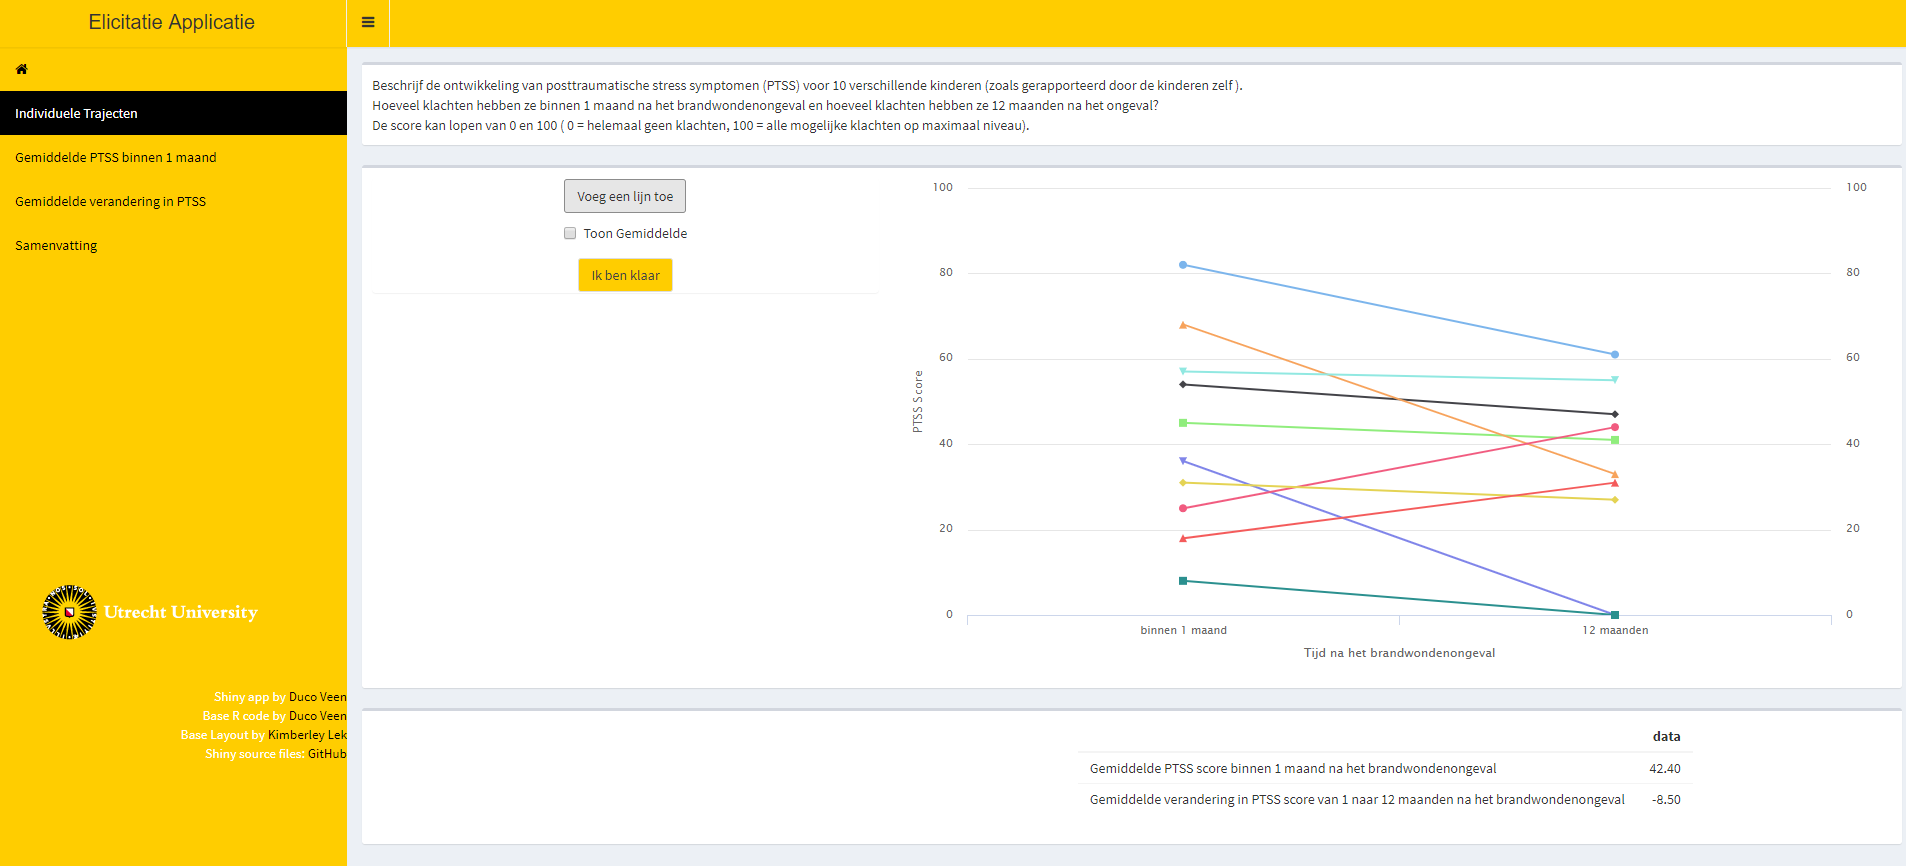
\includegraphics[width=0.9\linewidth]{figures/chapter_6/Figure2b} 

}

\caption{Step one of the elicitation procedure. Trajectories of PTSS development were elicited for 10 individuals that are representatitve for the population. From these trajectories point estiamtes for the average intercept and the average slope were obtained.}\label{fig:ch06fig2}
\end{figure}

\vspace*{2cm}

\begin{figure}

{\centering 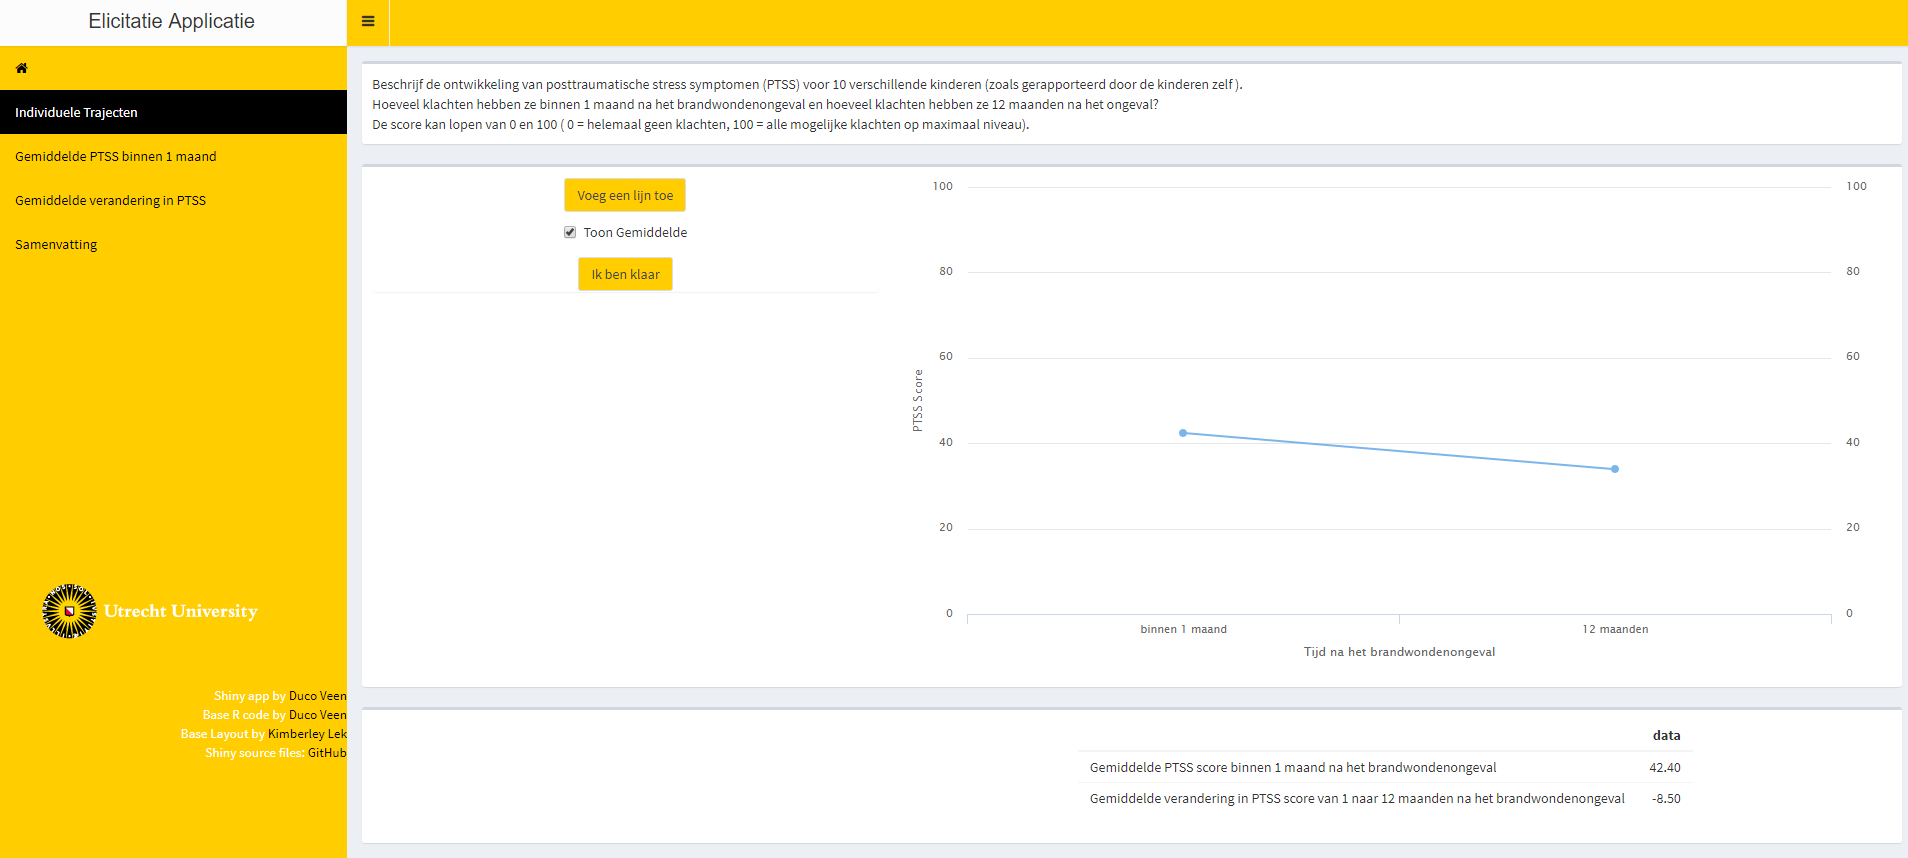
\includegraphics[width=0.9\linewidth]{figures/chapter_6/Figure3} 

}

\caption{Step two in the elicitation procedure, providing visual feedback on the extracted average trajectory based upon the experts' provided individual trajectories.}\label{fig:ch06fig3}
\end{figure}

\newpage

\begin{figure}[H]

{\centering 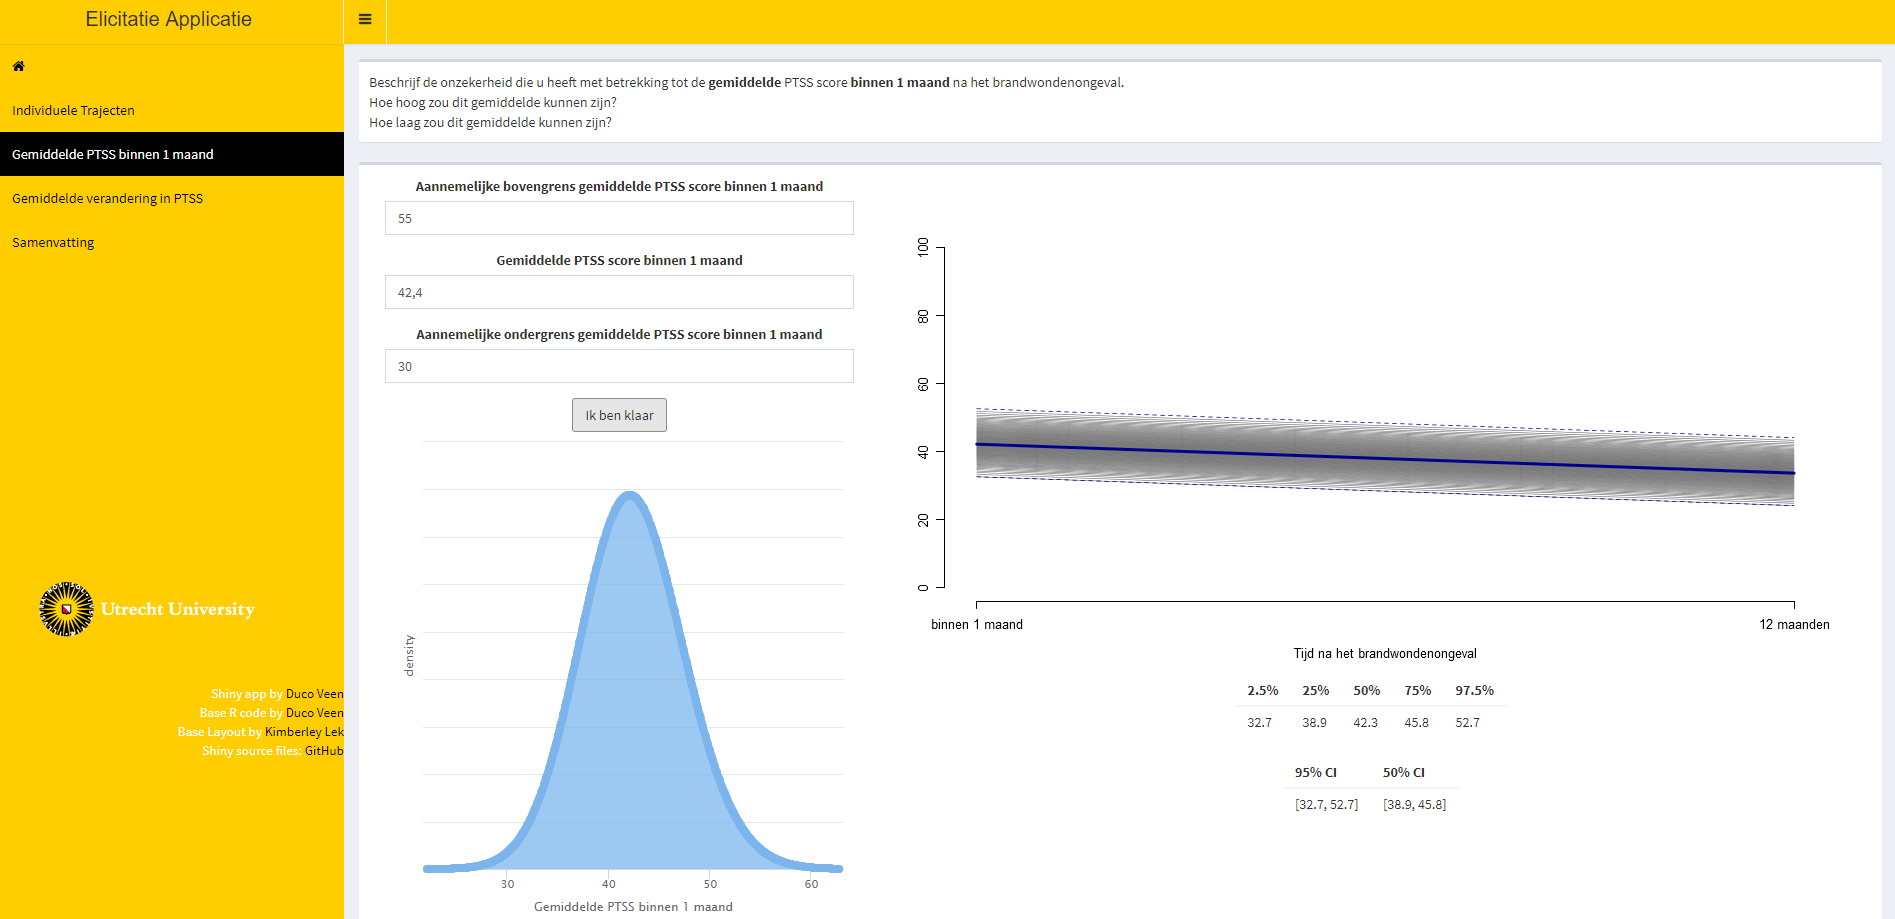
\includegraphics[width=0.9\linewidth]{figures/chapter_6/Figure4a} 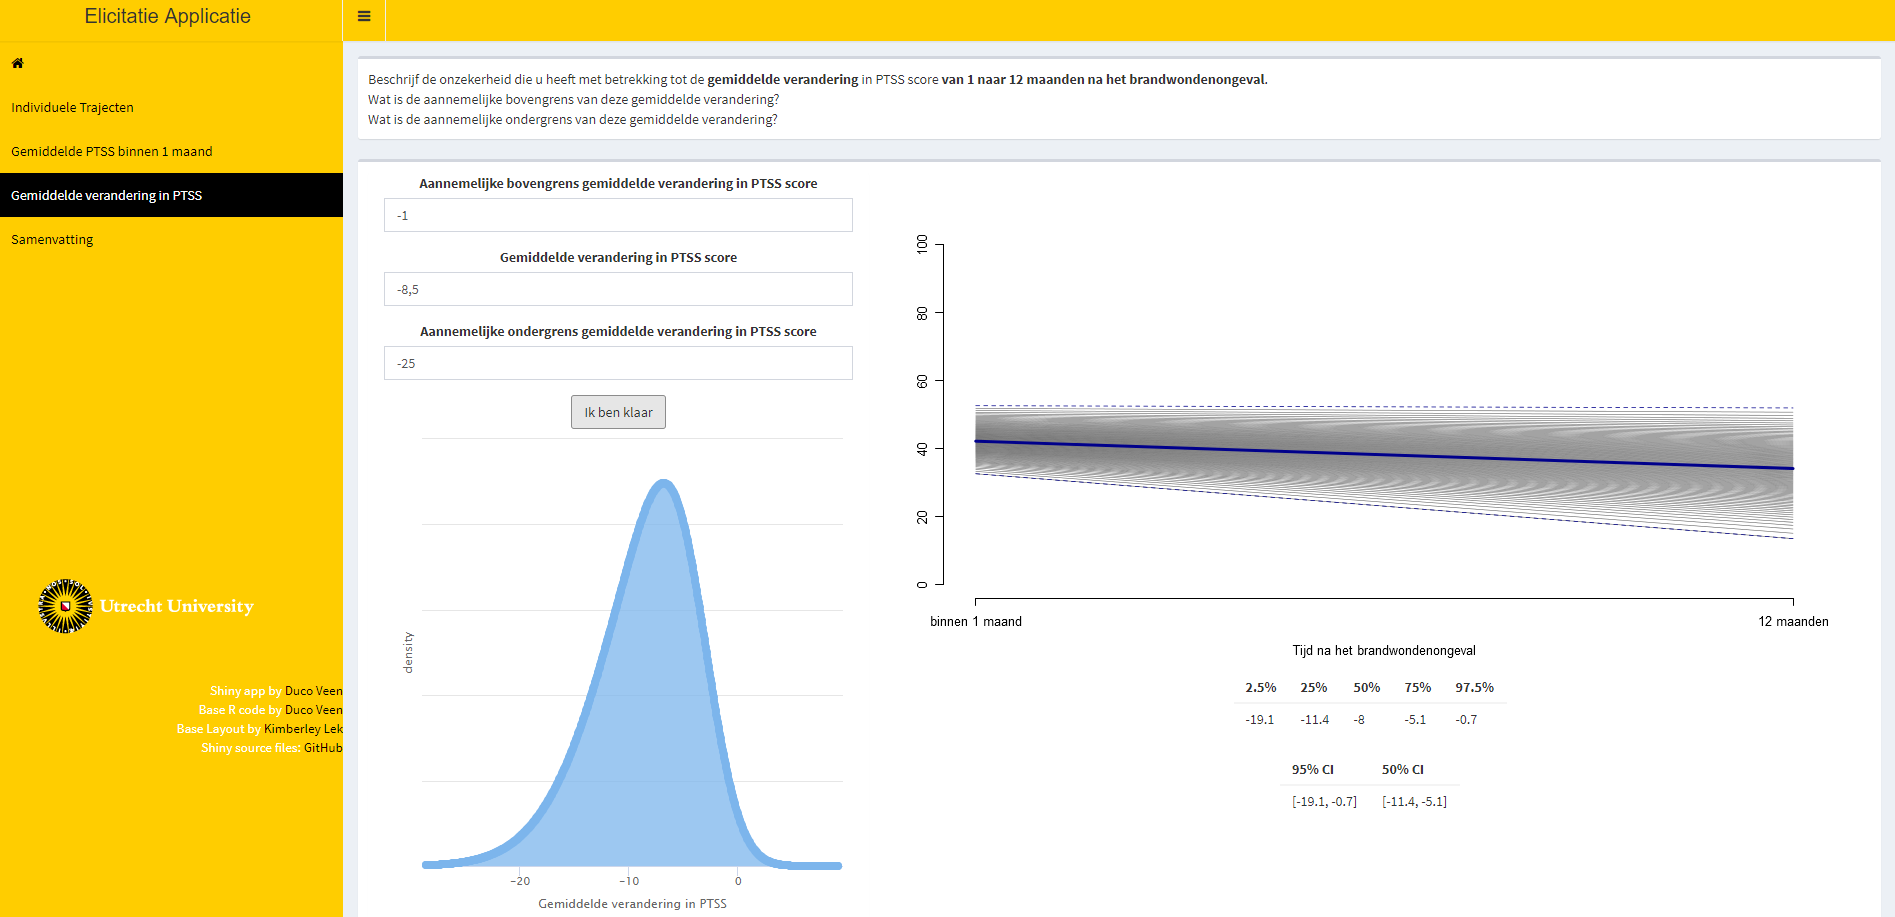
\includegraphics[width=0.9\linewidth]{figures/chapter_6/Figure4b} 

}

\caption{Steps three and four of elicitation procedure for the average intercept, top panel, and the average slope, bottom panel. The input that was required for step three was provided in the fields on the top left of the tab in the elicitation software. The single parameter feedback was provided on the bottom left of the tab, displaying the fitted distribution with respect to that parameter. The effect on the implied average trajectory was displayed on the right hand side of the tab. The average trajectory that was accepted in step two is diplayed and a gray band has been added around this average trajectory that represents the 95\% Credibility Interval (CI) for the average trajectory. In the top panel only the uncerainty with respect to the intercept was added to the average trajectory, in the bottom panel the uncertainty with respect to both the interecept and the slope was added.}\label{fig:ch06fig4}
\end{figure}

\begin{figure}[H]

{\centering 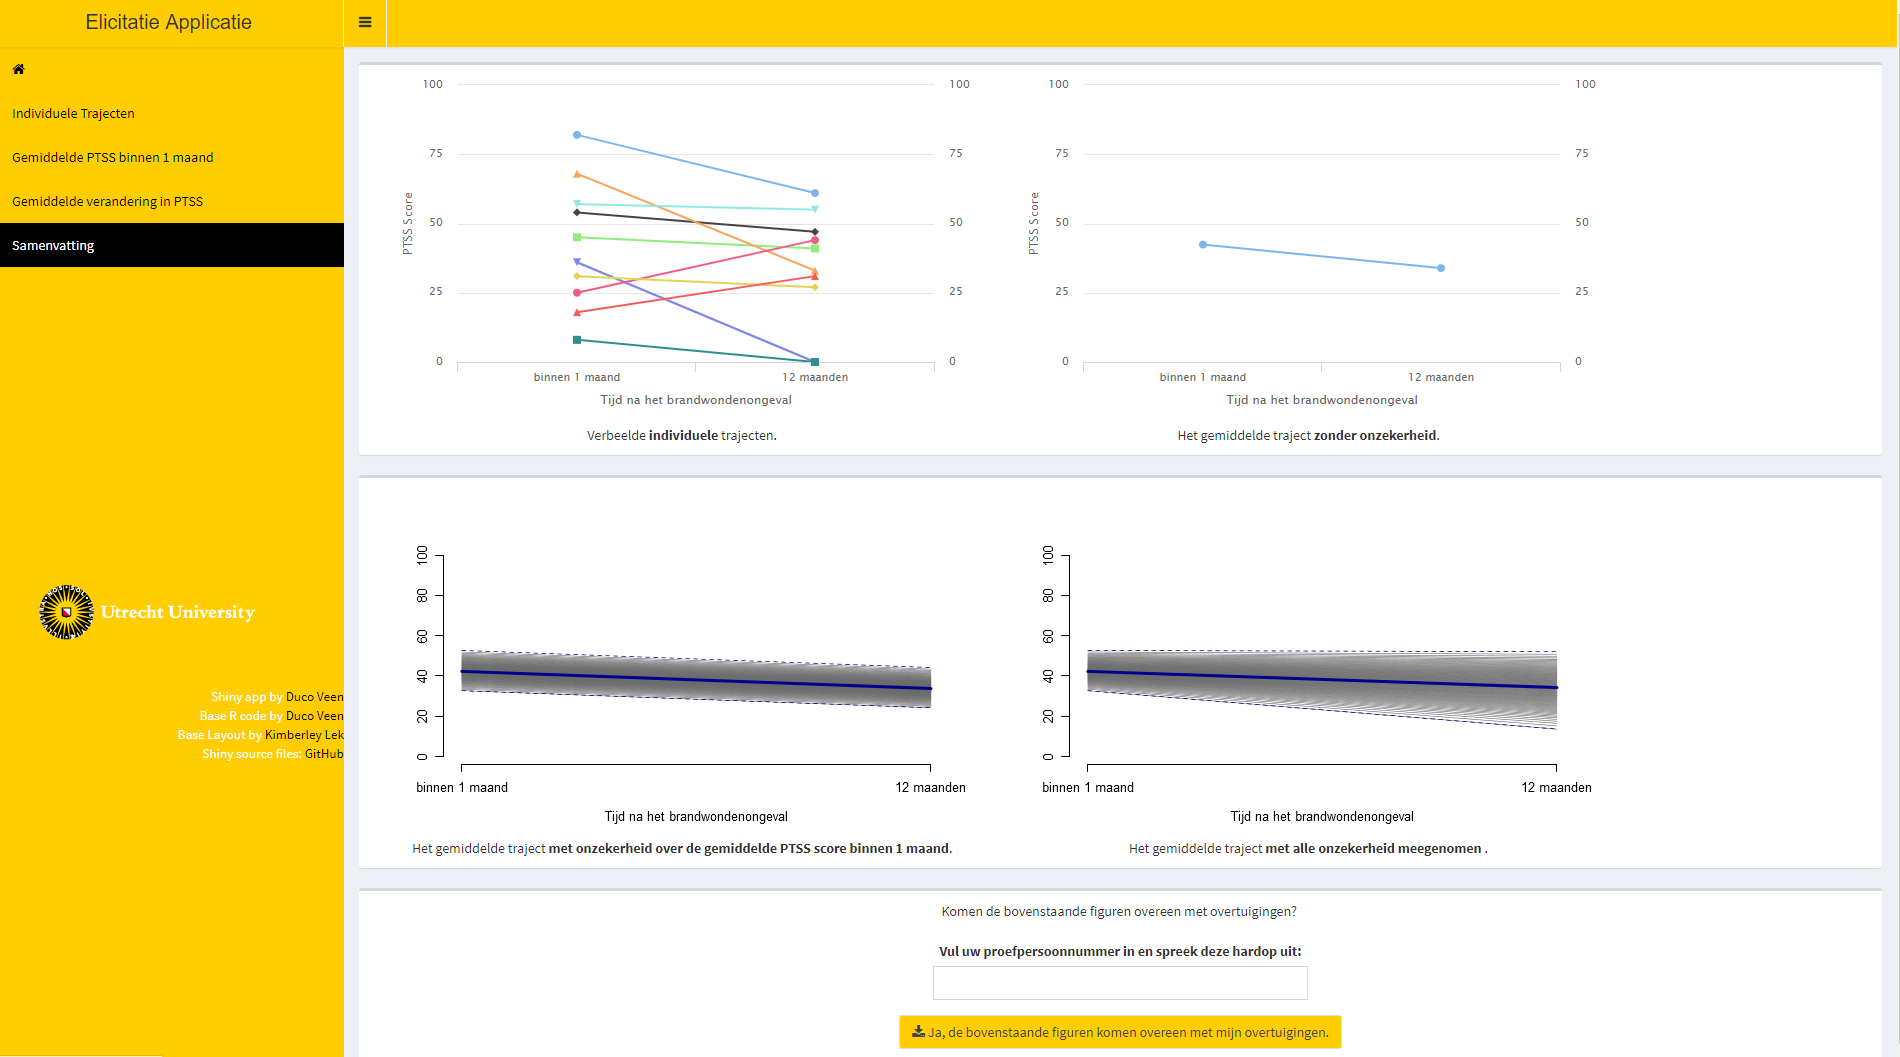
\includegraphics[width=0.9\linewidth]{figures/chapter_6/Figure5} 

}

\caption{Summary page of the elicitation procedure. The top left plot within the page displayed all individual trajectories that the expert specified. The top right plot displayed the average trajectory that was obtained based on those individual trajectories. The bottom left plot displayed the average trajectory with uncertainty (95\% CI) concerning the intercept value taken into account. The bottom right plot displayed the average trajectory with uncertainty (95\% CI) concerning both the intercept value and the slope value taken into account.}\label{fig:ch06fig5}
\end{figure}

\hypertarget{results-4}{%
\section{Results}\label{results-4}}

This section first covers a descriptive part on the expert judgements. We report the priors that the experts provided, the mixture priors that can be made from these expert judgements on an aggregated and group distinct level. Thereafter we report prior-data (dis)agreement measures for all individual expert judgements and the mixture distributions. These prior-data (dis)agreements are based upon the data that was collected in the prospective study by Egberts et al. (\protect\hyperlink{ref-egberts_mother_2018}{2018}). Finally, we report notable results from the audio recordings. Note that the quantitative results, analyses and an overview of individual expert judgements can be found via the OSF webpage for this project at \url{https://osf.io/y5evf/}. The transcripts of the audio recordings include many identifying characteristics with respect to both the experts and patients they described during the elicitation and to preserve privacy these are not available. This is in accordance with the ethical approval agreement.

\hypertarget{individual-and-group-expert-judgements}{%
\subsection{Individual and Group Expert Judgements}\label{individual-and-group-expert-judgements}}

All 14 expert judgement had been elicited allowing them to specify a skewed normal distribution parameterized according to Burkner (\protect\hyperlink{ref-burkner_parameterization_2019}{2019}). In Figure \ref{fig:ch06fig6} all the elicited individual expert distributions can be found as well as the mixture distributions\footnote{Note that the mixtures are based on normal approximations of the elicited skewed normal distributions due to computational instability of the mixture distributions when skewed normal expert priors where used.} for all experts, the psychologists group and the nurses group regarding both the mean intercept and the mean slope of PTSS development. From Figure \ref{fig:ch06fig6} it can be seen that the experts judgements differed quite substantially. Especially concerning the development of PTSS as expressed by the slope parameter we can see that actually expert disagreed on the direction of the effect and with a lot of confidence. When we look at the groups of experts an interesting pattern emerges. If we combine the expert judgements of the psychologists and the nurses into their respective groups the nurses turn out to have a substantially different view from the psychologists. Not only did the nurses' judgements express a higher initial amount of PTSS to be present in the population on average, their combined view also expressed that these initial PTSS scores are quite likely to increase on average over time. The psychologists in contrast assigned almost no probability to an increase in the average PTSS score over the time period of a year, see Figure \ref{fig:ch06fig7} for a closer look.

\hypertarget{prior-data-disagreement}{%
\subsection{Prior-Data (dis)Agreement}\label{prior-data-disagreement}}

To assess the (dis)agreement of experts' judgements with the data from the prospective study by Egberts et al. (\protect\hyperlink{ref-egberts_mother_2018}{2018}) we used Kullback-Leibler (KL) divergences (Kullback \& Leibler, \protect\hyperlink{ref-kullback_information_1951}{1951}) between the posterior distribution that is based upon the data and an uninformative benchmark prior and the individual and aggregated expert judgements. Using information theoretical distance measures to asses prior-data (dis)agreement in this manner has previously been discussed by for instance Bousquet (\protect\hyperlink{ref-bousquet_diagnostics_2008}{2008}), Lek \& Van De Schoot (\protect\hyperlink{ref-lek_how_2019}{2019}), and Veen et al. (\protect\hyperlink{ref-veen_using_2018}{2018}). KL-divergences provide us with an indication of how much information is lost is we approximate distribution \(\pi_1\) by another distribution \(\pi_2\). A higher divergence indicates a higher loss of information. In this case \(\pi_1\) will be the posterior distribution based upon the data and an uninformative benchmark prior, to which we refer as the reference posterior. We approximate the reference posterior with the elicited prior distributions and report the loss of information. For an overview of the priors that are used to compute the reference posterior see Figure \ref{fig:ch06fig8} and in Figure \ref{fig:ch06fig9} the reference posteriors for the group mean latent intercept and slope are visualized.

In addition to comparing the expert priors to the benchmark posterior we added two other comparisons to create a frame of reference. Two benchmark situations are added and their loss of information is calculated. In the situation of benchmark 1 we would take some information regarding the measurement instrument into account. The scale of the measurement instrument was standardized such that values are between 0 and 100, therefore a \(U(0, 100)\) prior on the group mean intercept would cover all possible parameter values. With the parameterization such that the final time measurement implies a change of one times the individuals latent slope parameter, taking the standardized scale into account a \(U(-100, 100)\) prior on the latent slope covers all possible parameter values and declares them equally possible. For benchmark 2 we take an extremely conservative approach and take two \(N(0, 10^8)\) priors on the latent group mean intercept and slope.

The KL-divergences are reported in \ref{tab:ch06tab1} and are the numerical representation of the loss of information that occurs by approximating the reference posteriors distributions from Figure \ref{fig:ch06fig9} by the distributions that can be seen in Figure \ref{fig:ch06fig7} for the experts priors. It seems that there are quite some experts that are in disagreement with the collected data from Egberts et al. (\protect\hyperlink{ref-egberts_mother_2018}{2018}). There are some individuals, notably experts 9 and 13, that provide a very similar view to the collected data, whilst some experts provide a similar view with respect to one of the two parameters, e.g.~experts 3 and 6. It is notable that the group of psychologists in particular and the group of experts as a whole show less loss of information with respect than the data than most experts on both parameters. Finally, what is noteworthy is that benchmark 1, which has no preference for any part of the parameter space covered by the measurement instrument, resembles the data more than most experts and more than the nurses as a group.

\hypertarget{audio-recordings}{%
\subsection{Audio Recordings}\label{audio-recordings}}

The following observations were noteworthy in the transcripts of the audio recordings. All psychologists referred back to the concept of PTSS specifically during the elicitation procedure. In the group of nurses we found a lot of mentioning of stress, but only two nurses actually referred back to PTSS specifically. Three psychologists reflected on the linearity assumption of the model and noted that non-linear trajectories often occur. Five of the nurses expressed sentiments that the more severe cases came to mind more easily and therefore might be over represented in their beliefs. Only one psychologists expressed a similar statement. Thee experts, one psychologist and two nurses, actively reflected on the visual feedback and adjusted their input in the elicitation tool based on this. One experts, a nurse, stated that although they were sure about the direction of the trajectory they felt unsure about the associated numerical representation. Finally, one expert, a nurse, repeatedly mentioned that they found the task hard to do.

\begin{figure}[H]

{\centering 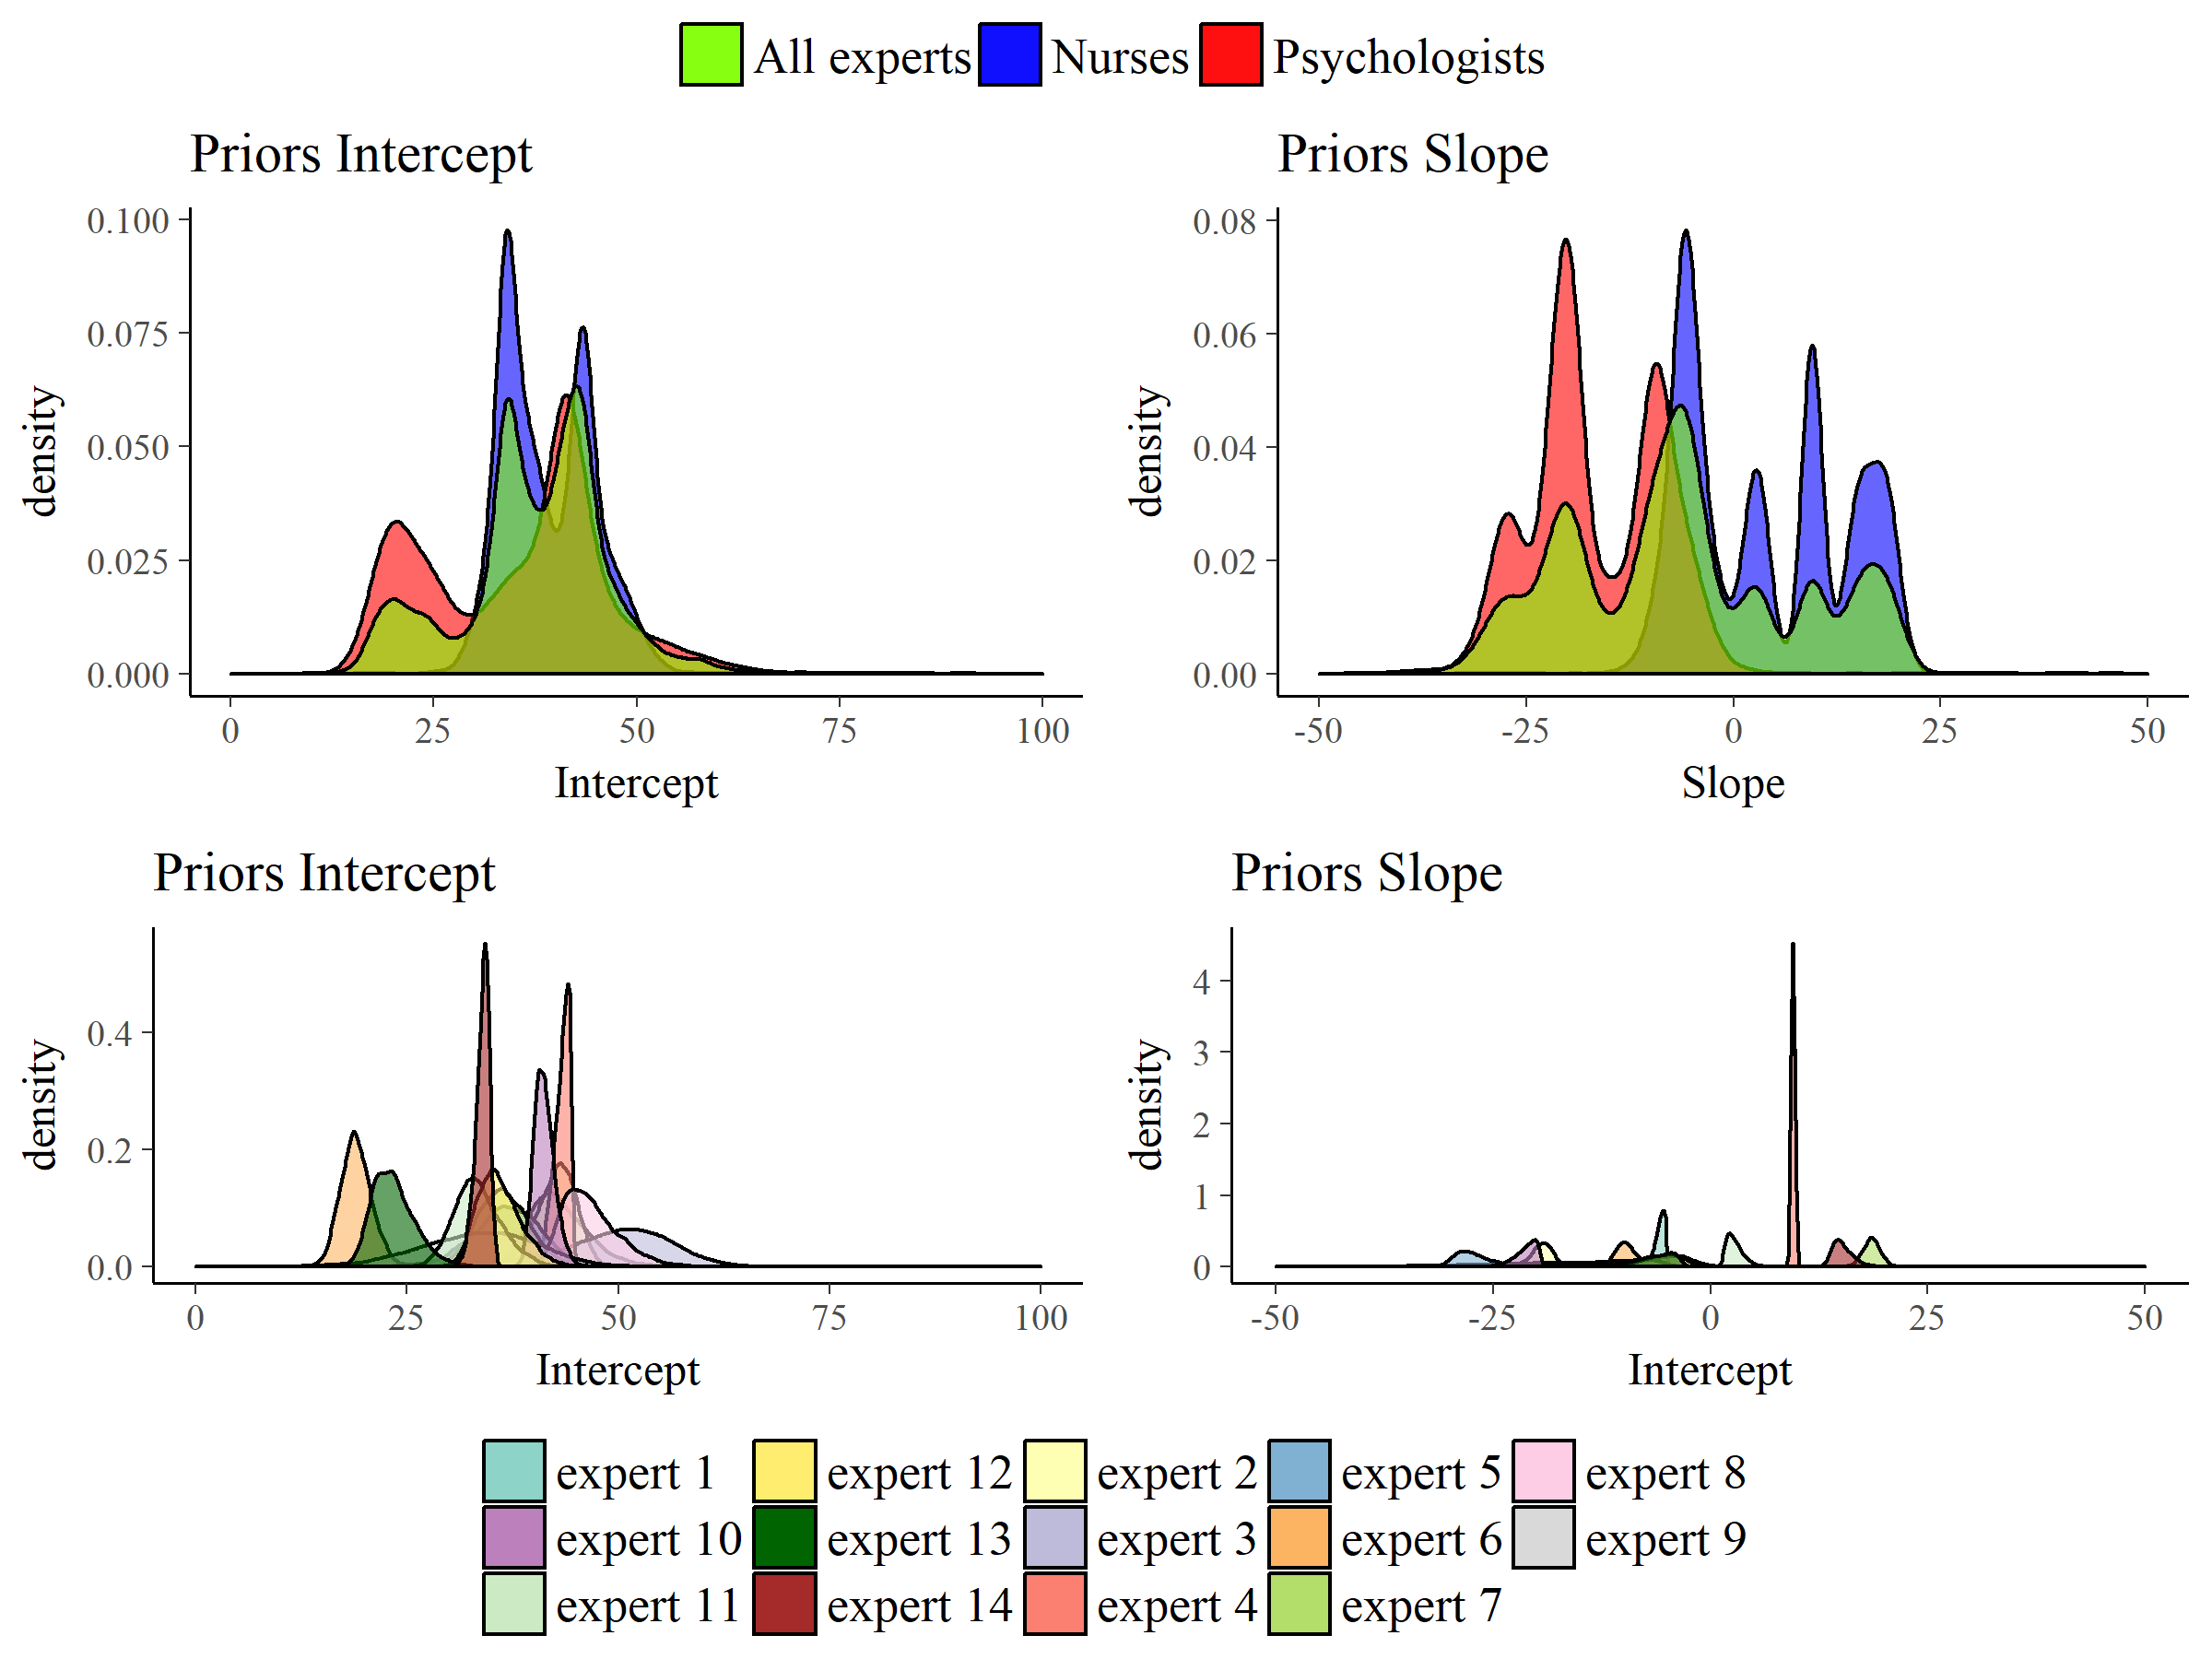
\includegraphics[width=1\linewidth]{figures/chapter_6/all_priors} 

}

\caption{Elicited prior distributions from all experts and the associated mixture priors for all experts, the psychologists group and the nurses group regarding both the mean intercept and the mean slope of PTSS development.}\label{fig:ch06fig6}
\end{figure}

\begin{figure}[H]

{\centering 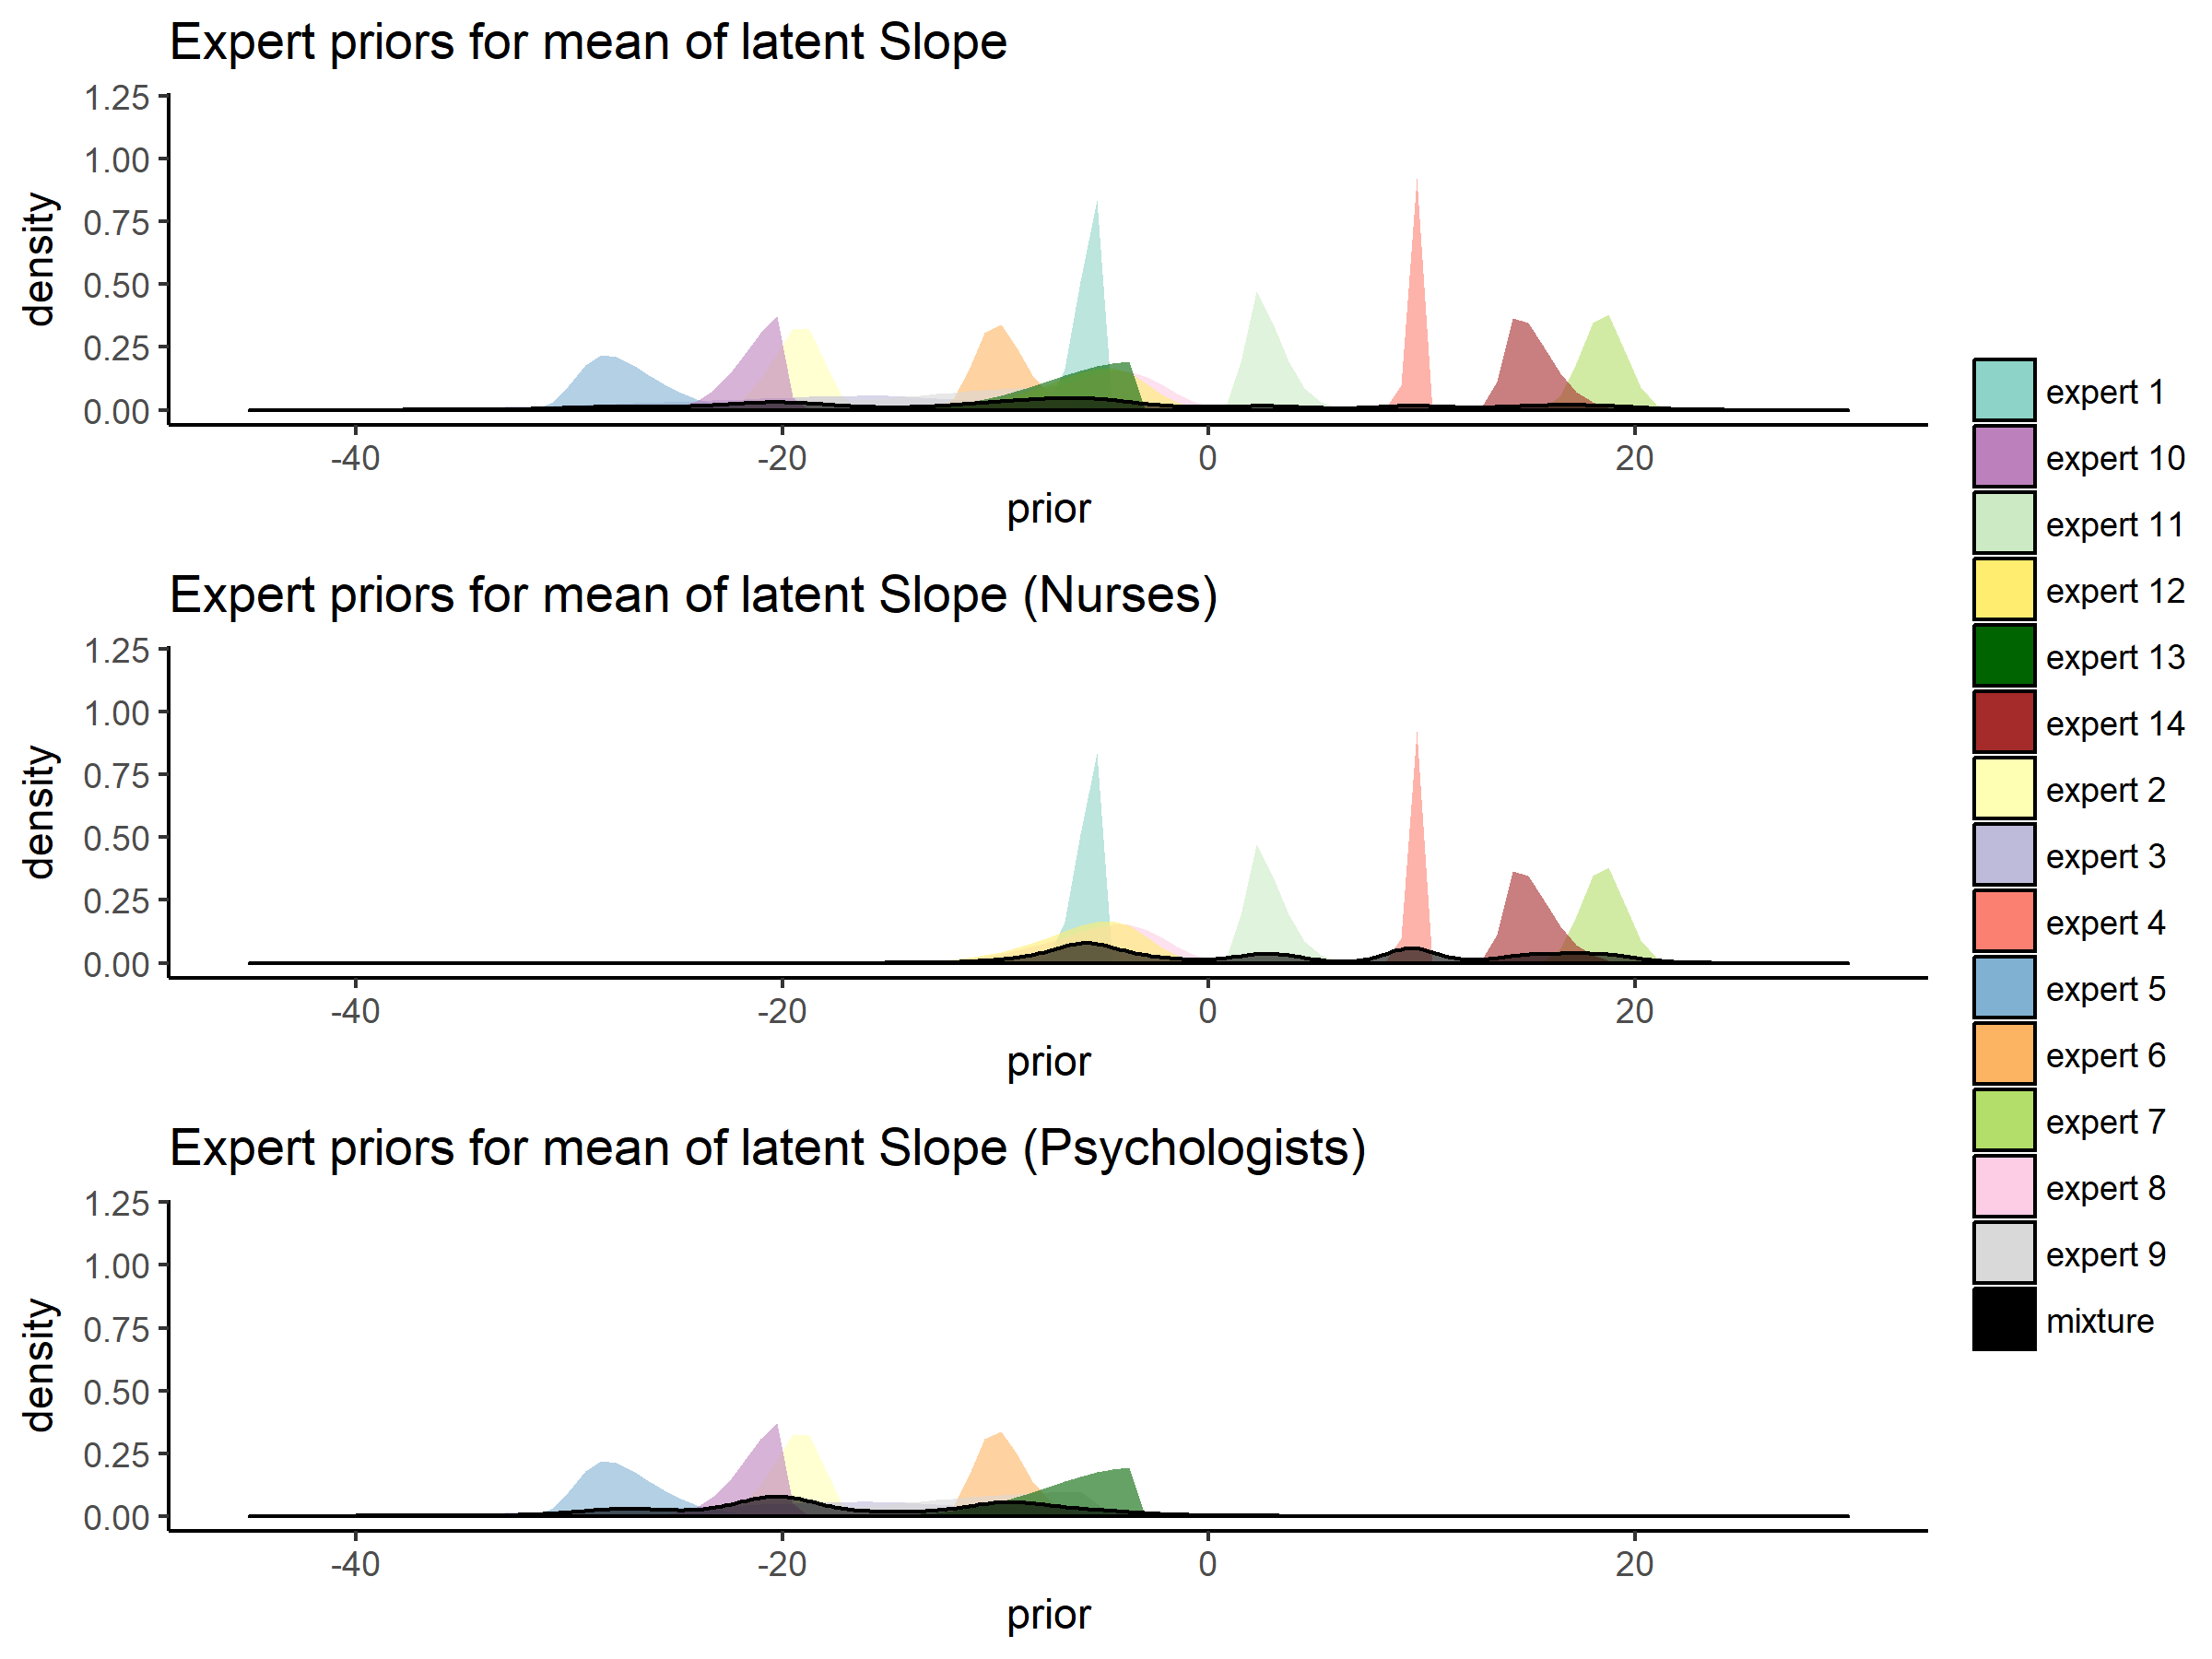
\includegraphics[width=0.85\linewidth]{figures/chapter_6/priors_experts_slope} 

}

\caption{Elicited prior distributions from all experts and the associated mixture priors for all experts, the psychologists group and the nurses group regarding the mean slope of PTSS development. There was a notable difference in expert judgements between the psychologists and the nurses groups.}\label{fig:ch06fig7}
\end{figure}



\begin{figure}[H]

{\centering 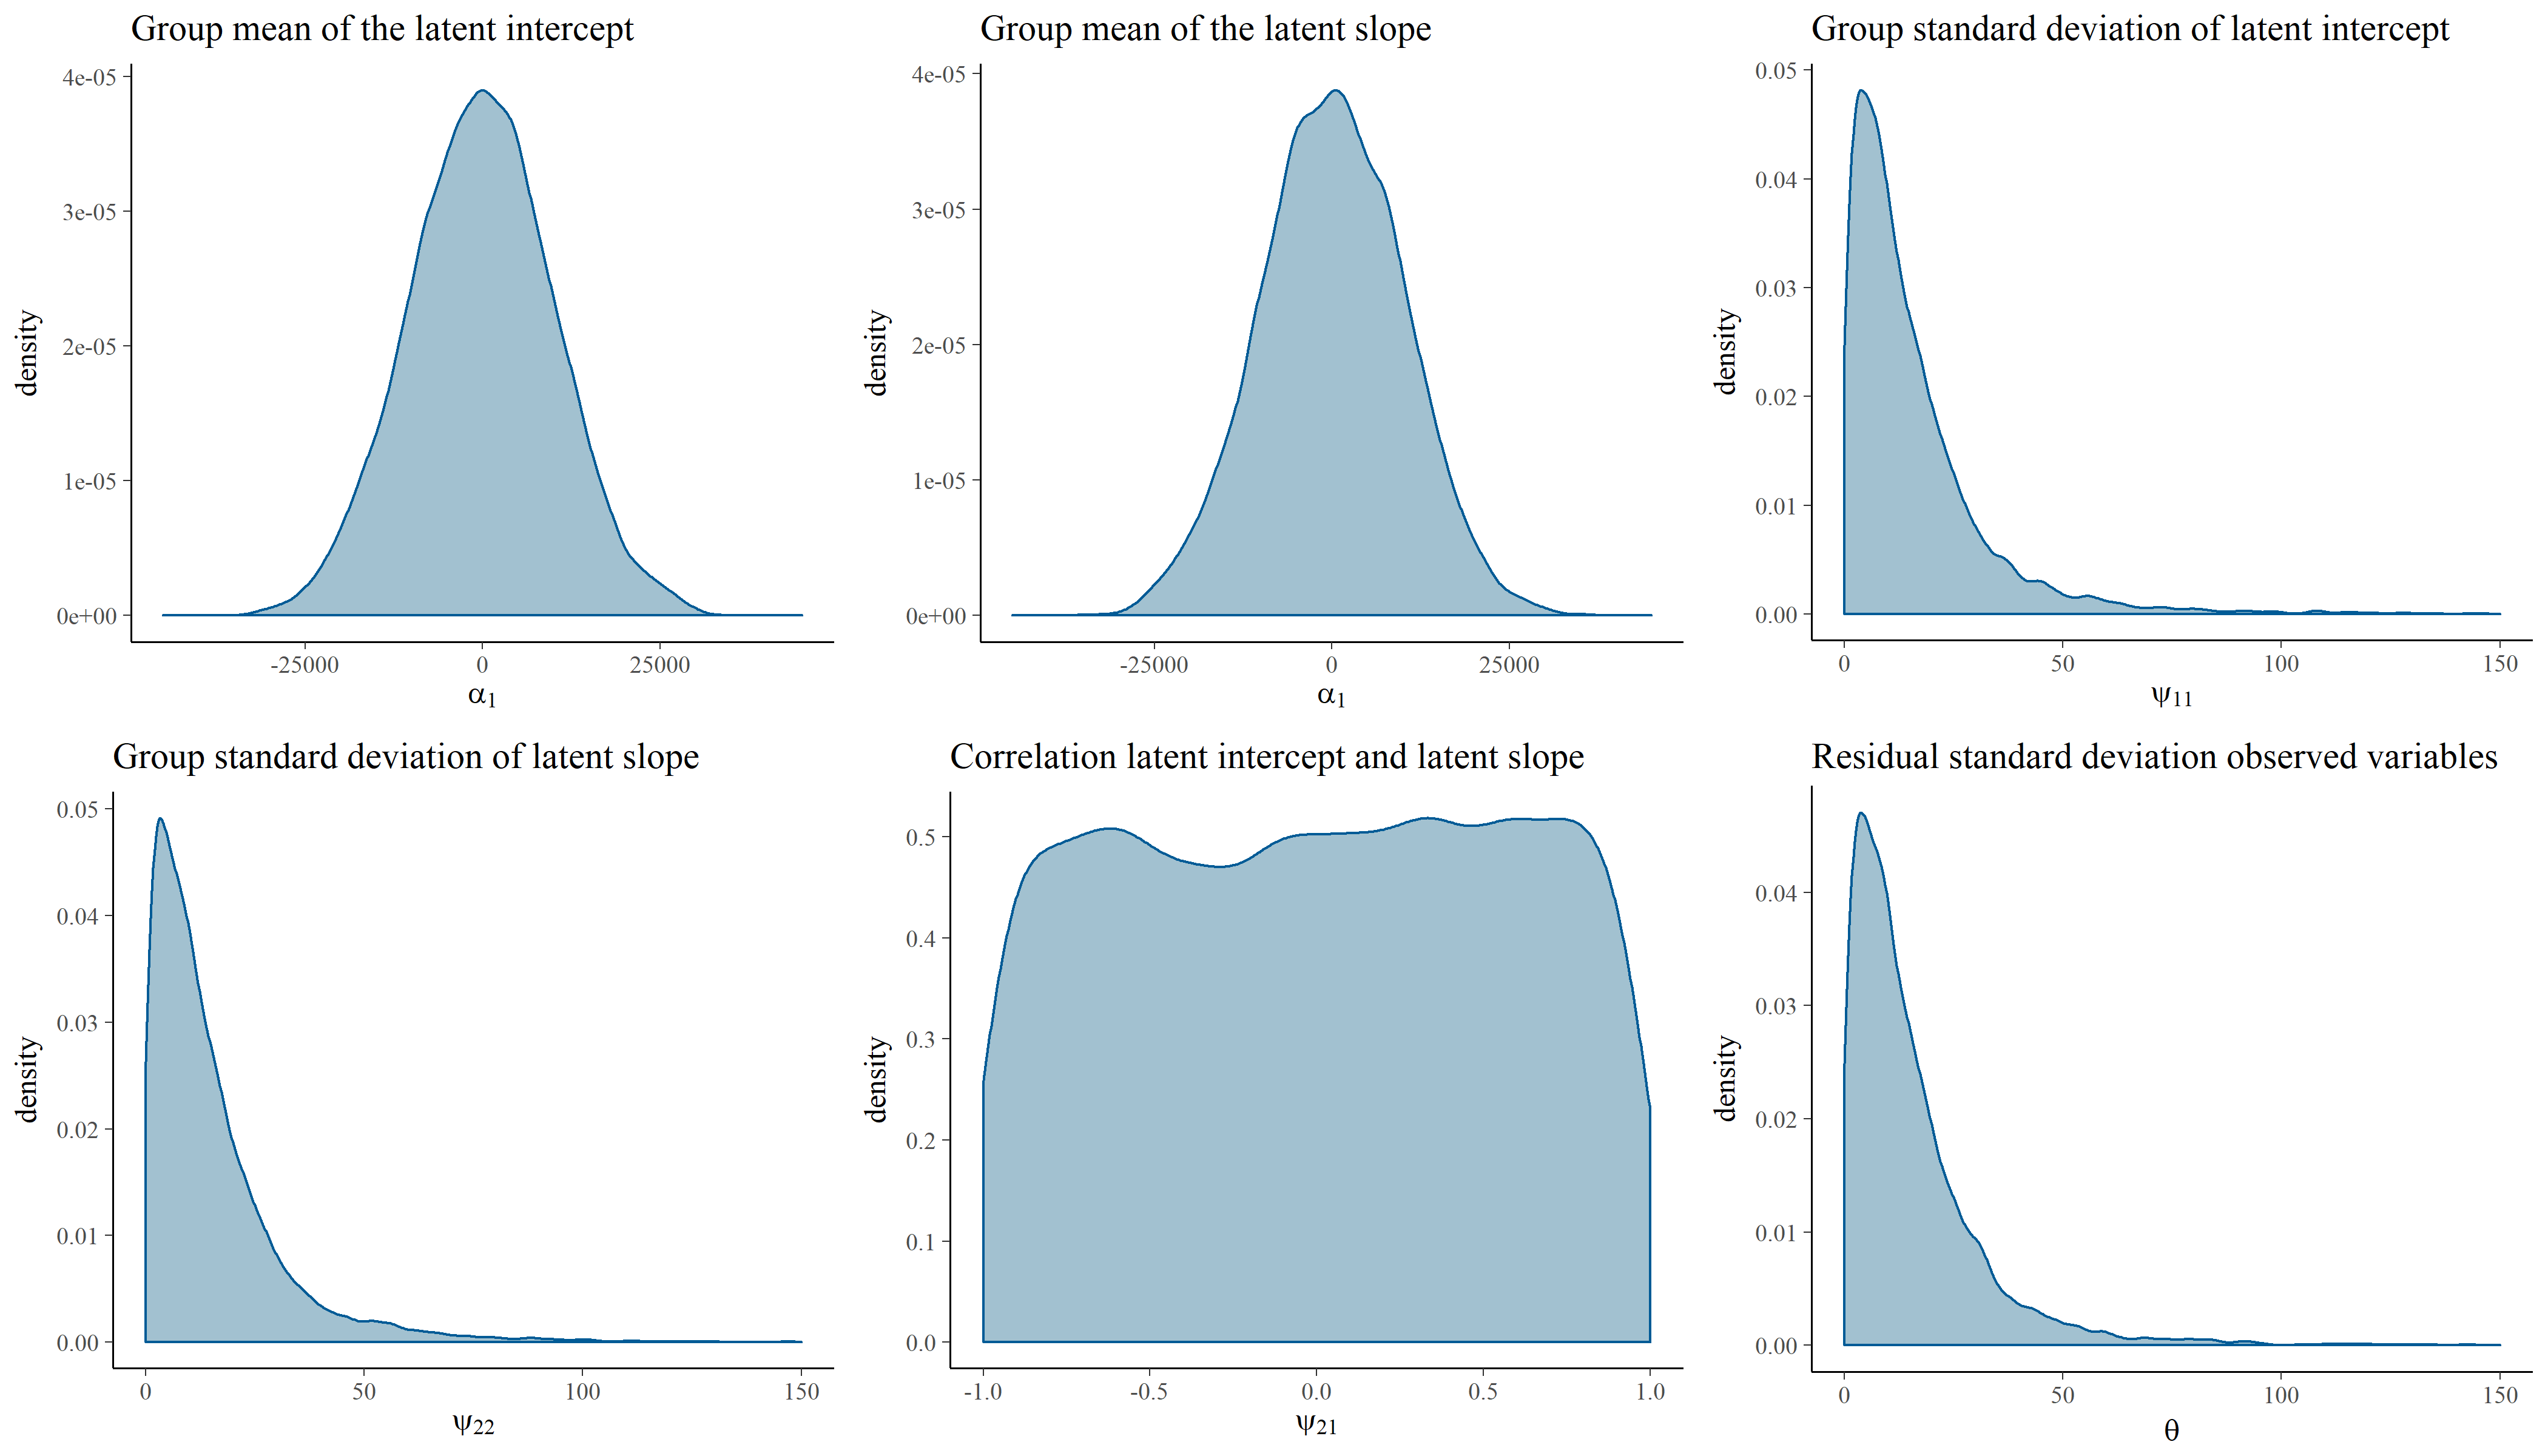
\includegraphics[width=1\linewidth]{figures/chapter_6/priors_reference} 

}

\caption{Visual representation of the prior distributions that are used to obtain the reference posterior. The prior distributions are \(\alpha_1 \sim N(0, 10^8)\), \(\alpha_2 \sim N(0, 10^8)\), \(\psi_{11} \sim half-t(3, 0, 196)\), \(\psi_{22} \sim half-t(3, 0, 196)\), \(\psi_{21} \sim U(-1, 1)\), and \(\theta \sim half-t(3, 0, 196)\).}\label{fig:ch06fig8}
\end{figure}



\begin{figure}[H]

{\centering 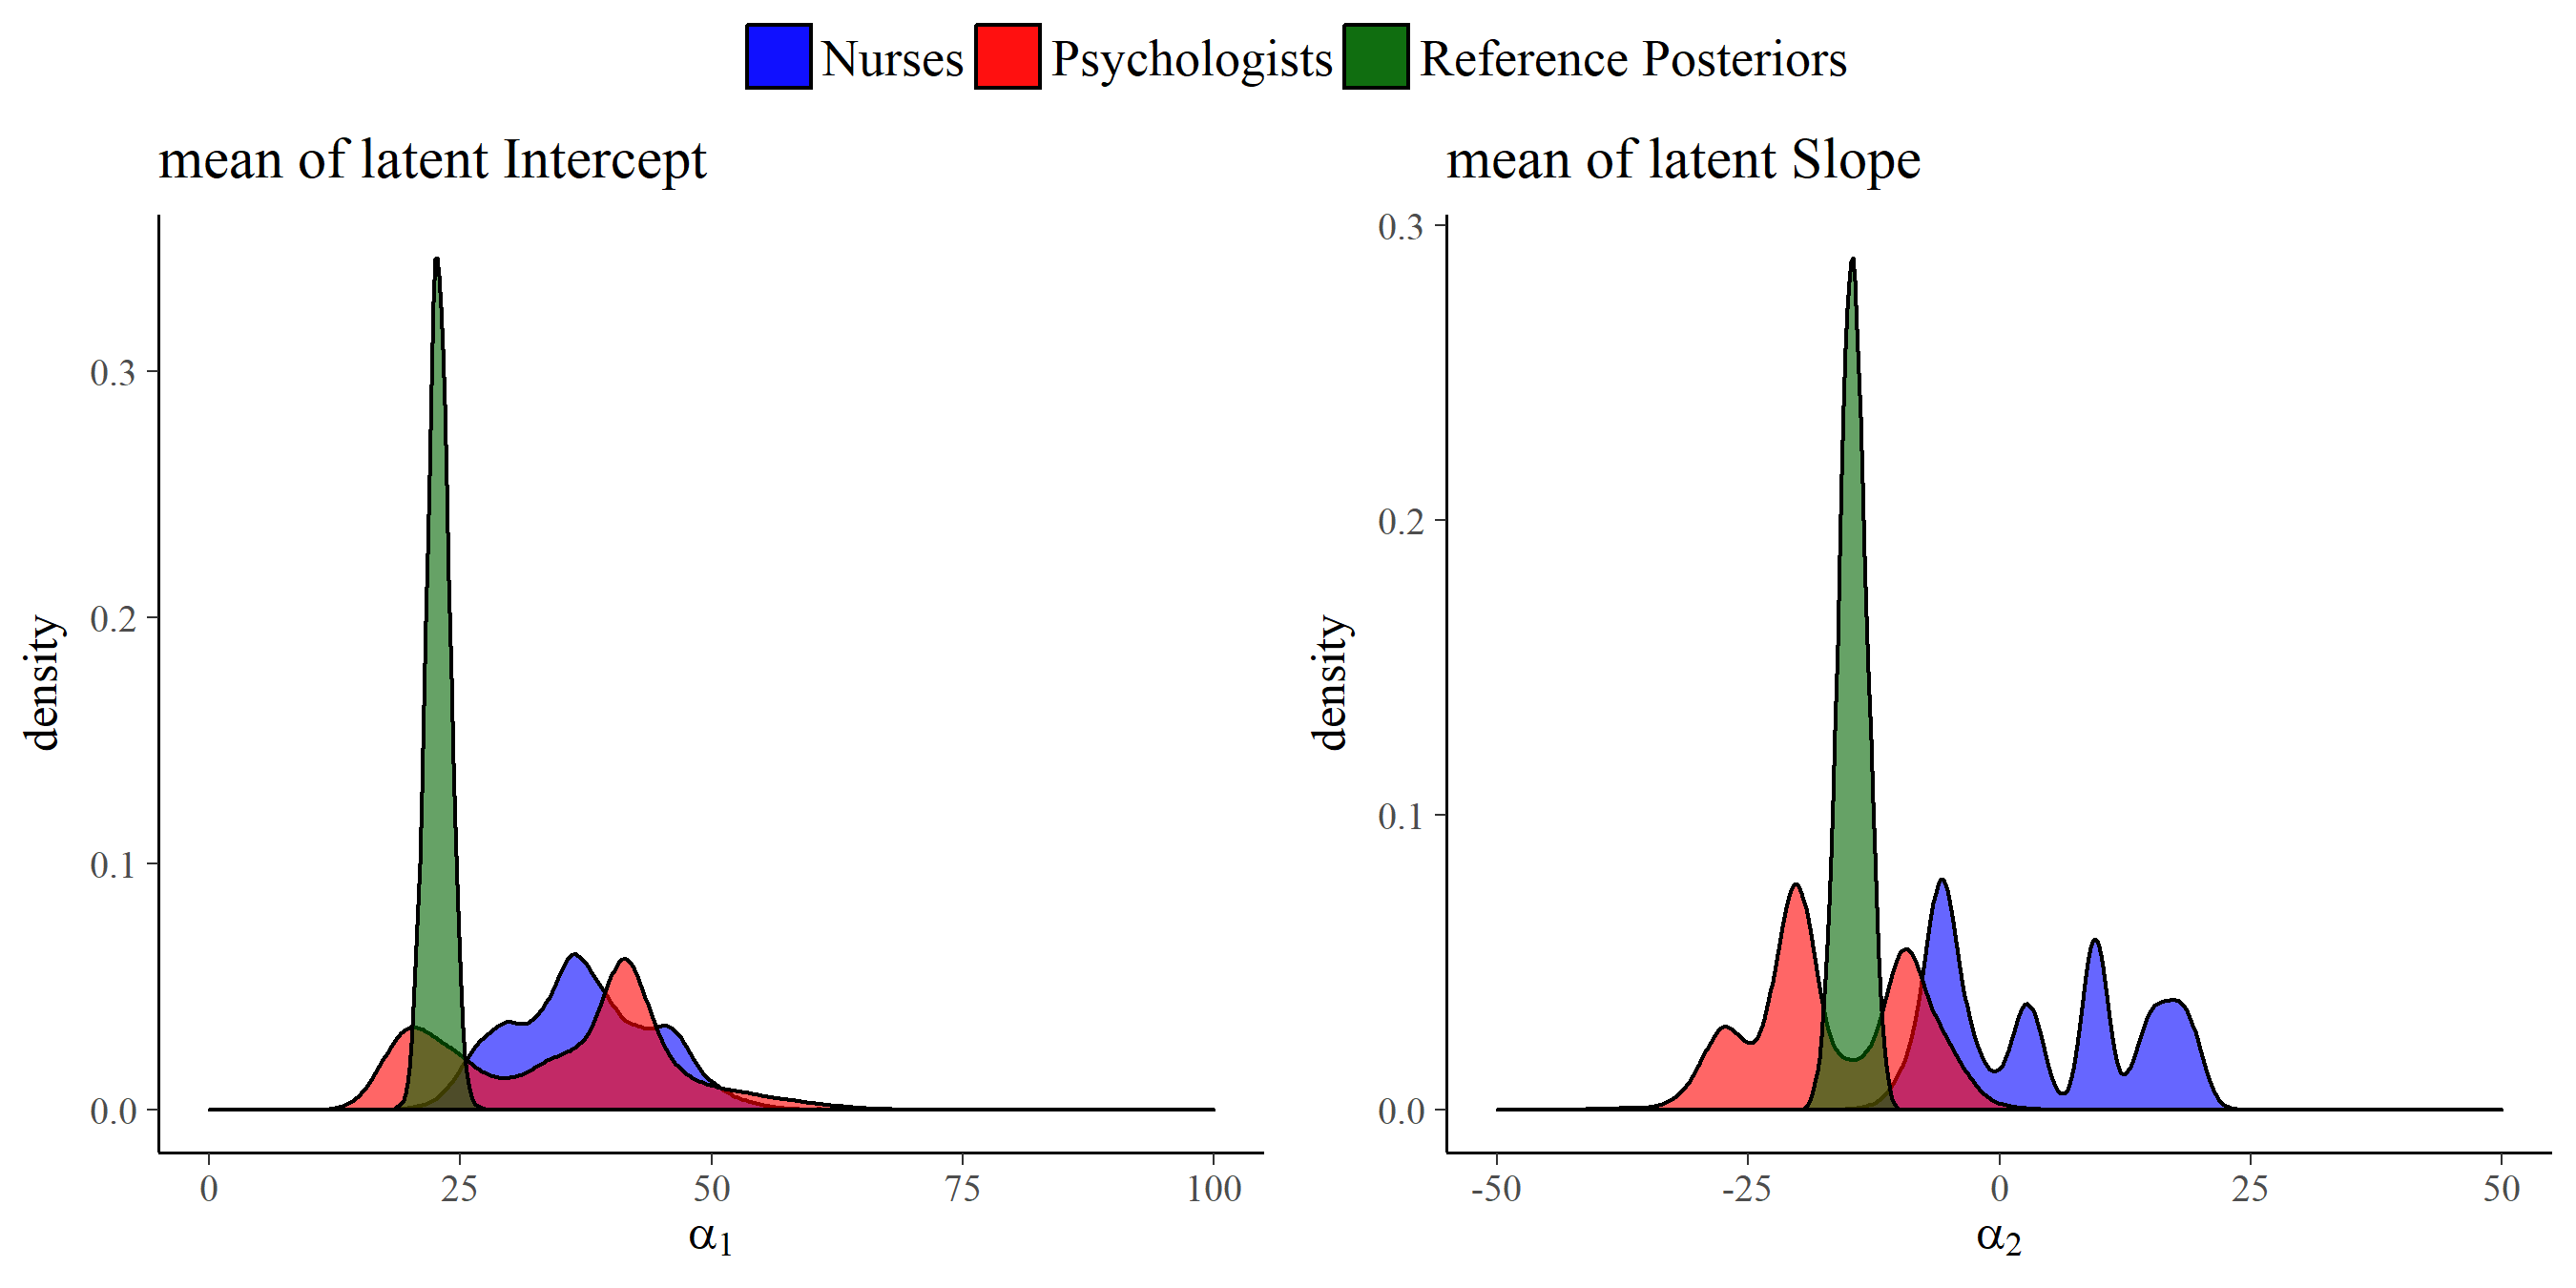
\includegraphics[width=1\linewidth]{figures/chapter_6/experts_vs_reference} 

}

\caption{Visual representation of the reference posterior distributions for the group mean of latent intercept and slope with the group expert priors for the parameters. The reference posteriors are approximately distributed \(\alpha_1 \sim N(22.7, 1.3)\), and \(\alpha_2 \sim N(-14.6, 1.9)\).}\label{fig:ch06fig9}
\end{figure}

\begin{table}

\caption{\label{tab:ch06tab1}Kullback-Leibler divergences for all individual and mixture priors to the reference posterior.}
\centering
\begin{tabular}[t]{lrr}
\toprule
  & Intercept & Slope\\
\midrule
Benchmark 1 & 3.04 & 3.56\\
Benchmark 2 & 8.56 & 8.39\\
Nurses & 8.19 & 5.88\\
Psychologists & 1.99 & 2.18\\
All & 2.72 & 2.63\\
\addlinespace
Expert 1 & 42.87 & 59.18\\
Expert 2 & 45.16 & 25.87\\
Expert 3 & 6.71 & 1.23\\
Expert 4 & 72.86 & 55.38\\
Expert 5 & 5.66 & 98.32\\
\addlinespace
Expert 6 & 2.10 & 22.17\\
Expert 7 & 79.20 & 59.61\\
Expert 8 & 46.97 & 4.37\\
Expert 9 & 2.48 & 1.28\\
Expert 10 & 43.74 & 67.55\\
\addlinespace
Expert 11 & 12.78 & 64.56\\
Expert 12 & 99.94 & 4.88\\
Expert 13 & 0.35 & 3.62\\
Expert 14 & 75.00 & 74.11\\
\bottomrule
\end{tabular}
\end{table}

\hypertarget{discussion-1}{%
\section{Discussion}\label{discussion-1}}

We were able to elicit expert judgements with respect to the development of PTSS in young burn victims from 14 experts and contrasted this with data collected in a traditional way by means of a questionnaire. This study demonstrated differences in views between experts. On an individual basis the experts were particularly in disagreement with regards to the change of PTSS one year post-burn. Many experts do not overlap with each other in their beliefs when we look at the elicited probability distributions for the slope parameter. The expert judgements not only differed from one individual to the next, but it may be that there is a relationship between the experts' role in the post-burn treatment process and their view on the childrens' development of PTSS. The two groups of experts notably differed in the aggregated elicited judgements. Moreover, the aggregated judgements of the psychologists seemed to align with the data collected by Egberts et al. (\protect\hyperlink{ref-egberts_mother_2018}{2018}) whilst the nurses judgements seemed to differ.

With respect to the differences between the two groups of experts the most remarkable difference was found with respect to the slope parameter. The aggregated views of the groups of experts result in distributions with more uncertainty compared to the individual experts' beliefs. The dispersed views of the experts put together ensure coverage of a larger part of the parameters space than the individual expert judgements do. Interestingly, the more uncertain distributions still clearly present a separation of the views regarding the development of PTSS in young burn victims between the nurses expert group on the one hand and the psychologists expert group and the data collected by Egberts et al. (\protect\hyperlink{ref-egberts_mother_2018}{2018}) on the other hand. The aggregated judgements from the psychologists assigned almost no probability to the group average PTSS increasing one year post-burn. The aggregated judgements from the nurses, in contrast, assigned a lot of probability to an increase of the group average PTSS one year post-burn. As there is no grounded truth that we cannot conclude which views are a better or worse representation. However, the results do indicate that the nurses and the psychologists are not in agreement on what happens with respect to the development of PTSS in young burn victims. The audio recordings of the elicitation settings provided a possible explanation for this important distinction. All psychologists at some point during the elicitation referred to, or specifically mentioned, the construct of PTSS. The group of nurses mentioned several sources of distress but only two nurses actually referred back to PTSS, one of which also judged the one year post-burn PTSS to decrease. As burn victims indeed can experience other sources of distress, e.g.~related to the development of scar tissue or operations they have to undergo, nurses might have convoluted PTSS symptoms with other patient symptoms. This could also explain why the aggregated nurses' view judged the initial PTSS level to be higher for the group average than the aggregated psychologists' view. Overall, the differences might reflect the fact that psychologists are trained to diagnose and treat PTSS, whereas nurses are primarily concerned with procedural and physical care for the patient, and are not responsible for diagnosing and treating PTSS.

Besides differences between the nurses and the psychologists we also found a substantial difference between the reference posteriors, that provided a representation of the data from Egberts et al. (\protect\hyperlink{ref-egberts_mother_2018}{2018}), and the aggregated nurses prior. In Figure \ref{fig:ch06fig9} it can be seen that the psychologists' views overlapped with the reference posteriors. The nurses' views however did almost not overlap with reference posteriors. This could also numerically be assessed, as was done with the KL-divergences in Table \ref{tab:ch06tab1}. Because the aggregated nurses prior had little overlap with the reference posteriors the Benchmark 1 priors, uniform priors that takes the information of the measurement instrument into account, outperformed this group in terms of loss of information. This implies the data collected by Egberts et al. (\protect\hyperlink{ref-egberts_mother_2018}{2018}) was better approximated by an uninformed expression of the measurement properties of the questionnaire than by the nurses' group prior. The children in the study by Egberts et al. (\protect\hyperlink{ref-egberts_mother_2018}{2018}) expressed a lower quantity of PTSS in their self-reported questionnaires compared to the nurses' expert judgements on PTSS symptoms for this populations. There can be several explanations for this discrepancy, first the questionnaire might have resulted in underreporting of symptoms, a view also expressed by one of the experts. In line with this, Egberts et al. (\protect\hyperlink{ref-egberts_mother_2018}{2018}) found that mothers gave higher ratings of their child's PTSS compared to the children themselves, although mothers' ratings also appeared to be influenced by their own symptoms of PTSS. Also, fathers did not report higher ratings of PTSS compared to their children. Alternatively, the discrepancy could be explained by the elicitation of the expert judgements. Especially the nurses group reported higher PTSS levels compared to the self-reports and the previously mentioned convolution of symptoms and lack of specific knowledge about PTSS might be a cause for this observation. In the recordings of the elicitation settings we found another possible cause. Five of the nurses expressed sentiments that the more severe cases came to mind more easily and therefore might be overrepresented in their beliefs. This is a clear expression of the well known availability heuristic (Tversky \& Kahneman, \protect\hyperlink{ref-tversky_availability:_1973}{1973}) that can cause biases in elicitation studies (O'Hagan et al., \protect\hyperlink{ref-ohagan_uncertain_2006}{2006}). In the psychologists group only a single expert expressed a similar remark. The availability heuristic, if not remedied, might cause the discrepancy between the reference posteriors and the expert judgements.

The study showed that providing visual feedback on the representation of the experts' beliefs can lead to adjustments by the experts to their input such that obvious incorrect representations of the experts' beliefs are remedied. Unfortunately it is not possible to validate that the representation of the experts' beliefs is actually the ``true'' beliefs of the expert (Colson \& Cooke, \protect\hyperlink{ref-colson_expert_2018}{2018}; O'Hagan et al., \protect\hyperlink{ref-ohagan_uncertain_2006}{2006}). However, one of the main reasons to use elicitation software is to ameliorate the effects of heuristics and biases by getting experts to actively reflect on the probability distribution that will be used to represent their beliefs. In the recordings three experts actively reflect on their distributions and adjust them based on the visual feedback and for this the purpose the elicitation software seems to have worked well. Nevertheless, it seems from our current study that even with the graphical feedback, some experts might still suffer from overconfidence, see Figure \ref{fig:ch06fig6}. Expert 11, for instance, stated \emph{``\ldots{} of course, I have a lot of uncertainty anyway.''}. However, this does not seem reflected in the elicited distribution which has a 99\% CI for the latent intercept {[}27.2, 41.7{]} and the latent slope {[}1.2, 5.9{]}. As the experts were only available to us for a limited time we did not provide a specialized training aimed at elicitation and overcoming heuristics associated with elicitation tasks which might be a limitation for the current study, and the associated (individual level) results.

This study indicated that aggregating expert judgements could potentially mitigate the severity of the individual biases, as one thereby relies less on single, possibly overconfident, experts. The aggregation of all experts' judgements, or only the psychologists' judgements, lead to less discrepancy between the traditionally collected data and the elicited beliefs than mostly any individual expert and the benchmarks. Aggregating or pooling of expert judgements into a single distribution is common in elicitation studies and can be done in several manners. In our current study we used opinion pooling with equal weights (O'Hagan et al., \protect\hyperlink{ref-ohagan_uncertain_2006}{2006}, Chapter 9). Alternatively, there is much literature on how expert judgements could be weighted in the aggregation of views. The classical model (Cooke, \protect\hyperlink{ref-cooke_experts_1991}{1991}, Chapter 12) is one of the foremost examples of this. In the classical approach calibration questions are used to assess the experts. Based on the calibration questions experts' judgements on the target question, or question of interest, are weighted to together form the groups weighted prior beliefs. The calibration questions should be related to the question of interest and their answers should be known but not to the experts (Colson \& Cooke, \protect\hyperlink{ref-colson_expert_2018}{2018}). It is recommended to have at least eight to ten calibration questions if dealing with continuous variables (Cooke, \protect\hyperlink{ref-cooke_experts_1991}{1991}, Chapter 12). The experts are elicited concerning the question of interest and the calibration questions. Their answers on the calibration questions are evaluated against the known true values and the experts are rated on their informativeness and accuracy (Colson \& Cooke, \protect\hyperlink{ref-colson_expert_2018}{2018}; Cooke, \protect\hyperlink{ref-cooke_experts_1991}{1991}). The ratings of the weighting components is based upon the idea of KL-divergences (O'Hagan et al., \protect\hyperlink{ref-ohagan_uncertain_2006}{2006}, Chapter 9) such as we used to compare the experts' judgements against the collected data on the question of interest directly. As far as we know there have not been any studies using the classical approach in the social sciences. Finding calibration questions turns out to be a hard problem, as knowing the true answer to these questions is required. We described the KL-divergence between the target question and the experts' judgements, but calibrating experts based on these weight would be putting emphasis on the traditionally collected data twice. As the traditionally collected data might suffer from biases too, consider for instance the total survey error framework (Groves et al., \protect\hyperlink{ref-groves_survey_2011}{2011}, Chapter 2) including nonresponse error and measurement error, this double emphasis might not be desirable. Instead, our equal weights aggregation approach relied on the inclusion of experts with balance in views and diversity in backgrounds (Cooke \& Goossens, \protect\hyperlink{ref-cooke_procedures_1999}{1999}).

In conclusion, it is possible to express the experts' domain knowledge as prior distributions using the described methodology and compare these elicited distributions to traditionally collected data. The individual expert judgements in general show quite some discrepancy in comparison to traditionally collected data, although there are notable exceptions to this. When taking the mixtures of the groups of experts the discrepancy becomes less pronounced, very much so for the psychologists group. The psychologists mixture prior has less KL-divergence than mostly any individual expert and notably less KL-divergence than benchmark 1, the uniform prior that takes the information of the measurement instrument into account. The expert judgements add information to the research area and exploring (dis)similarities between expert judgements and traditional data open up two exciting avenues for future research. First, the collection of data on the experts that might be predictive for the amount of KL-divergence they exhibit with respect to traditionally collected data. Second, the organisation of a Delphi like setting with all experts after the individual judgements are collected and compared with traditional data. The group setting can provide insights into the reasons behind the discrepancies between traditional collected data, individual experts and groups of experts. Predicting and explaining (dis)similarities between experts judgements and traditional data such as results of questionnaires can be a potential new line of research for the social sciences.

\newpage

\hypertarget{conflicts-of-interest}{%
\section*{Conflicts of Interest}\label{conflicts-of-interest}}
\addcontentsline{toc}{section}{Conflicts of Interest}

The authors declare that the research was conducted in the absence of any commercial or financial relationships that could be construed as a potential conflict of interest.

\hypertarget{ethics-statement}{%
\section*{Ethics Statement}\label{ethics-statement}}
\addcontentsline{toc}{section}{Ethics Statement}

This study was carried out in accordance with the recommendations of the internal Ethics Committee of the Faculty of Social and Behavioural Sciences of Utrecht University, with written informed consent from all subjects. All subjects gave written informed consent in accordance with the Declaration of Helsinki. The protocol was approved by the internal Ethics Committee of the Faculty of Social and Behavioural Sciences of Utrecht University.

\hypertarget{acknowledgements-1}{%
\section*{Acknowledgements}\label{acknowledgements-1}}
\addcontentsline{toc}{section}{Acknowledgements}

The authors are grateful to all experts for their invested time and energy.

\hypertarget{funding}{%
\section*{Funding}\label{funding}}
\addcontentsline{toc}{section}{Funding}

This work was supported by Grant NWO-VIDI-452-14-006 from the Netherlands Organization for Scientific Research. None of the funders or sponsors of this research had any role in the design and conduct of the study; collection, management, analysis, and interpretation of data; preparation, review, or approval of the manuscript; or decision to submit the manuscript for publication.

\hypertarget{thesisdiscussion}{%
\chapter{Discussion}\label{thesisdiscussion}}

\chaptermark{DISCUSSION}
\thispagestyle{empty}

The \protect\hyperlink{introduction}{introduction of this thesis} started by explaining Bayesian statistics as a way of updating information. I start this discussion by reflecting on the example that I used in Chapter \protect\hyperlink{introduction}{1}, discussing the importance of (hidden) assumptions, and I relate this to possible differences between experts and data. I consider different roles that expert knowledge can play in research, and under what conditions I think those roles could be appropriate. Finally, I give consideration to what seems a natural future direction for (my) research; decision making.

\hypertarget{hidden-assumptions}{%
\section{Hidden assumptions}\label{hidden-assumptions}}

In Chapter \protect\hyperlink{introduction}{1} the example of coin tosses is used to introduce the concept of Bayesian statistics, even though in the remainder of this thesis the normal distribution is used in the analyses. Why then, not explain Bayesian statistics using the normal distribution? The main reason is that the coin tossing example requires a single parameter \(\theta\), resulting in a straight-forward single-parameter model. Two parameters should be considered with respect to the normal distribution: the mean (\(\mu\)) and variance (\(\sigma^2\)). This makes explanations more complex and the interactions between the two parameter might not make for an intuitive initial framework. Many text books decide to first explain the situation in which either \(\mu\) or \(\sigma^2\) is fixed (e.g.~Albert, \protect\hyperlink{ref-albert_bayesian_2009}{2009}; Gelman et al., \protect\hyperlink{ref-gelman_bayesian_2013}{2013}; Kaplan, \protect\hyperlink{ref-kaplan_bayesian_2014}{2014}; Kruschke, \protect\hyperlink{ref-kruschke_doing_2010}{2010}; Lynch, \protect\hyperlink{ref-lynch_introduction_2007}{2007}; Ntzoufras, \protect\hyperlink{ref-ntzoufras_bayesian_2011}{2011}; Press, \protect\hyperlink{ref-press_subjective_2009}{2009}). This decision is taken consciously, which is illustrated by the following comments.

\begin{quote}
``For the purpose of mathematical derivation, we make the unrealistic assumption
that the prior distribution is either a spike on \(\sigma\) or a spike on \(\mu\).''

Kruschke (\protect\hyperlink{ref-kruschke_doing_2010}{2010}) p.~322
\end{quote}

\begin{quote}
``Perhaps a more realistic situation that arises in practice is when the
mean and variance of the normal distribution are unknown''

Kaplan (\protect\hyperlink{ref-kaplan_bayesian_2014}{2014}) p.~28
\end{quote}

\newpage

\begin{quote}
``In reality, we typically do not know \(\sigma^2\) any more than we know \(\mu\),
and thus we have two quantities of interest that we should be updating with
new information''

Lynch (\protect\hyperlink{ref-lynch_introduction_2007}{2007}) p.~65
\end{quote}

There is nothing wrong with explaining a simplistic version first. One reason not to do so is because an explanation with this `unrealistic' or `hidden' assumption might not make for proper intuition. In general, the more complex models become, the more complex specifying prior information becomes. Almost never is the specification of prior information as easy as in the examples in Chapter \protect\hyperlink{introduction}{1} concerning the coin flips and the Beta distribution that has a natural interpretation in that case. Moreover, in multiparameter models the priors interact with one another to say something about the data that you might expect. Priors on certain parameters by themselves might look reasonable, but together they can sometimes imply very implausible situations about reality. Simulating fake data, or looking at implied predictive distributions as done in Chapter \protect\hyperlink{Burns}{5}, can help identify these problems (Gabry, Simpson, Vehtari, Betancourt, \& Gelman, \protect\hyperlink{ref-gabry_visualization_2019}{2019}; Schoot et al., \protect\hyperlink{ref-van_de_schoot_tutorial_2020}{2020}). Moreover, recent work points to interpretation challenges for the prior if context of the likelihood is not taken into account (Gelman et al., \protect\hyperlink{ref-gelman_prior_2017}{2017}), or information about an experiment is ignored (Kennedy, Simpson, \& Gelman, \protect\hyperlink{ref-kennedy_experiment_2019}{2019}). Note in relation to this, how in the hierarchical model of Chapter \protect\hyperlink{Hierarchical}{4}, priors on the individual level are essentially based on the estimated group level effects, which includes information from both the prior and the likelihood. All this reflection on assumptions is not to criticize explanations in textbooks or articles. The point is made to highlight that the choices that are made with respect to the models and priors are highly influential for results and interpretations, and being explicit about them is a minimal requirement.

\hypertarget{expert-knowledge}{%
\section{Expert Knowledge}\label{expert-knowledge}}

Being transparent about models, priors and choices is related to the issue of eliciting expert knowledge. As mentioned in the introduction of Chapter \protect\hyperlink{DAC1}{3}, when conducting an elicitation experts are forced to use a representation system that belongs to the statistical realm. They are forced to use the same parametric representation as the statistical model. For non-trivial problems, statistical models can become complex quickly. If expert knowledge is elicited with the purpose of being used as a prior distribution in a statistical model, the implicit assumption is made that the expert adheres to the same model as statistically specified. This can be a rather strict assumption, in which confidence will decrease when models become more complex.

In this dissertation in Chapters \protect\hyperlink{DAC1}{3} and \protect\hyperlink{elicitlgm}{6} we focus on the comparison of experts' elicited distributions among one another and their contrast with respect to what traditional data implies given our statistical model. If discrepancies occur between the two this can be highly informative and it need not be that one or the other is at fault and wrong. The discrepancies are so interesting because the differences can occur due to different implied models. When discussing with experts why their beliefs diverge from one another, or from the traditional data, we can learn subtle differences in the implied models that experts use. The information obtained using experts-data (dis)agreements methodology might inform us to specify slightly different statistical models or include other variables in our statistical models. In the long run, if the experts learn from the data, and the model is refined based on expert knowledge, we can expect both sources of information to converge.

Note that I reflect here on cases where we do have data, not on cases where expert knowledge is used when no data is available. Obviously in those cases we do not have the luxury of comparing multiple sources of information. It is often more desirable to have any information, for instance provided by experts, than no information. In this scenario it is even more essential to have quality checks available to evaluate experts' expertise. As discussed in Chapter \protect\hyperlink{elicitlgm}{6}, the classical method is a much used procedure in this instance (Cooke, \protect\hyperlink{ref-cooke_experts_1991}{1991}, Chapter 12). The lack of suitable calibration questions for many social scientific research topics makes this method, at least for now, unfeasible in those settings. Moreover, the work presented in this dissertation is not a substitute for asking calibration questions, but should be viewed as an additional area of research.

In cases where calibration is possible, updating the elicited experts' beliefs with new data in a full Bayesian framework can certainly be considered. In cases where calibration is not an option, I would rather contrast expert knowledge as an alternative source of information than update it with traditionally collected data. The two alternative ways of incorporating information in prior distributions that were discussed in Chapter \protect\hyperlink{introduction}{1}, using previous research and logical constraints, seem more defensible than elicited expert priors without calibration. Especially the use of priors describing plausible parameter space seems no more than logical. In Chapters \protect\hyperlink{DAC1}{3} and \protect\hyperlink{elicitlgm}{6} we use uniform priors as benchmarks that could be considered in line with Laplace's (1749-1827) principle of insufficient reason. It seems that these might be more in line with the data in the proposed statistical model than some experts' beliefs. Whatever the reason, and whichever source of information is right, when using Kullback-Leibler divergences that assign truth status to the traditional data, the `ignorant' benchmarks examples resonate the following idea:

\begin{quote}
``Ignorance is preferable to error and he is less remote from the truth who
beliefs noting than he who believes what is wrong.''

Thomas Jefferson (1781)
\end{quote}

\hypertarget{taking-a-decision}{%
\section{Taking a decision}\label{taking-a-decision}}

I began this thesis by stating that all of us have to make decisions whilst facing uncertainty and incomplete information. In addition, I stated that Bayesian statistics offers a way to describe our state of knowledge in terms of probability. In this thesis we have indeed concerned ourselves mainly with obtaining prior, and estimating posterior, distributions of probability. We have contrasted sources of information, seeing this as an opportunity to learn and improve our knowledge and models. In short, we have concerned ourselves in this thesis with ways to systematically organize uncertainty and incomplete information, but not yet with the decision making process that should naturally follow from this.

Two approaches that are often used in science to make a decision, or come to a conclusion, are model selection and hypothesis testing. Model selection is a very useful concept to refine our theory and models. However, it does not always lead to a decision. Hypothesis testing is more naturally focused at making decisions, e.g.~can we reject the hypothesis that there is no effect? It seems, however, to be a rather unhelpful restriction to single out one value and contemplate the issue with respect to that value. Indeed, Bayesian estimation can be seen as a case in which we test an infinite number of hypotheses concerning which values are most likely for parameters (Jaynes, \protect\hyperlink{ref-jaynes_probability_2003}{2003}, Chapter 4). Moving beyond simple one dimensional questions to decisions that determine a course of action, it seems straightforward that we need to consider more than just an existence of an effect or not. Consider such questions as; do we implement a certain intervention in schools or not? Or should I get a certain type of insurance? To determine a course of action we need to be able to assess which choice seems most preferable out the options that are open to us. This cannot be assessed unless we assign value judgement to certain outcomes and take costs into account. Is raising the IQ of children by 1 point on average worth the investment if that means that we have to cut funding to hospitals by the same amount? Does the good outweigh the bad? That is the relevant question, not: should we change the way we teach at schools because an experiment provided us with \(p<.05\) for a hypothesis stating that both methods of teaching were exactly equal? The following words express this sentiment in a delightful way:

\begin{quote}
``You cannot decide what to do today until you have decided what to do with the tomorrows that today's decisions might bring.''

Lindley (\protect\hyperlink{ref-lindley_understanding_2013}{2013}), p.~249
\end{quote}

To extend the framework of Bayesian estimation into the field of decision making seems natural via the concepts of utility and loss. Given that a model has been found that seems reasonable, e.g.~via model selection, the inference solutions obtained by applying probability theory only provide us with a state of knowledge concerning parameters, it does not tell us what to do with that information (Jaynes, \protect\hyperlink{ref-jaynes_probability_2003}{2003}, Chapter 13). Utility or loss functions can be defined and maximized to determine which decision is optimal (Goldstein, \protect\hyperlink{ref-goldstein_subjective_2006}{2006}; Jaynes, \protect\hyperlink{ref-jaynes_probability_2003}{2003}, Chapter 13). Moreover, if sequential decisions should be taken, a decision tree should be made taking all information up to each point into account (Gelman et al., \protect\hyperlink{ref-gelman_bayesian_2013}{2013}, Chapter 9; Lindley, \protect\hyperlink{ref-lindley_understanding_2013}{2013}, Chapter 10). Utility can be defined very transparently, but it is not free of subjective value judgement (Jaynes, \protect\hyperlink{ref-jaynes_probability_2003}{2003}, Chapter 13). For a wonderful example that illustrates this, see Jaynes (\protect\hyperlink{ref-jaynes_probability_2003}{2003}), p.~400 - 402 on the differences in rationale and utility of insurance, viewed from the standpoints of the insurance agency, a poor person, a rich person, and a rich person with an aversion to risk. For a full decision analysis of different strategies in the context of risk reduction of lung cancer in relation to household environmental risk of exposure to radon gas, see Gelman et al. (\protect\hyperlink{ref-gelman_bayesian_2013}{2013}) p.~246-256.

In no way am I saying that assigning utility and loss functions are easy concepts. Moreover, I will not claim to have the wisdom at this point to undertake such an elaborate evaluation and ensure wise decisions. However, if I had to take a decision on what to peruse next academically, using what I have learned from working on this dissertation, I would peruse decision making. But only after I reflected on what tomorrows today's decision would bring, given the uncertain and incomplete information that I have.

\pagestyle{headings}

\makeatletter
\renewcommand\chaptermark[1]{%
    \markboth{\MakeUppercase{#1}}{}
}
\makeatother

\hypertarget{nederlandse-samenvatting}{%
\chapter*{Nederlandse Samenvatting}\label{nederlandse-samenvatting}}
\addcontentsline{toc}{chapter}{Nederlandse Samenvatting}

%
    \markboth{\MakeUppercase{NEDERLANDSE SAMENVATTING}}{}

\thispagestyle{empty}

\markboth{NEDERLANDSE SAMENVATTING}{NEDERLANDSE SAMENVATTING}

Iedereen moet beslissingen maken op basis van incomplete en onzekere informatie. Om ons te helpen de beschikbare informatie te organiseren en interpreteren maken we gebruik van statistiek. Bayesiaanse statistiek is een veelgebruikt conceptueel raamwerk dat kan helpen om de geschikte stappen te bepalen voor de toekomst. Dit statistische raamwerk is een kernonderdeel van deze dissertatie en wordt in alle hoofdstukken gebruikt.

Bayesiaanse statistiek bied de mogelijkheid om de huidige staat van kennis te beschrijven in termen van waarschijnlijkheid (Jaynes, \protect\hyperlink{ref-jaynes_bayesian_1996}{1996}). Meer dan dat, het kan worden gezien als een extensie van logica (Jaynes, \protect\hyperlink{ref-jaynes_probability_2003}{2003}). Het beschrijft bovendien hoe we zouden moeten leren van nieuwe informatie (Lindley, \protect\hyperlink{ref-lindley_understanding_2013}{2013}). Bayesiaanse statistiek stelt dat we kansverdelingen kunnen gebruiken om onze huidige staat van kennis over een parameter te beschrijven. Dit kunnen we doen voordat we nieuwe data observeren, dan heet dit een \emph{a priori} kansverdeling, ofwel voorkennis. Nadat we nieuwe data hebben geobserveerd werken we onze beschrijving van de staat van kennis bij tot een zogeheten \emph{a posteriori} kansverdeling.

Doordat voorkennis wordt uitgedrukt in termen van kansverdelingen bied dit de mogelijkheid om hier op verschillende manieren invulling aan te geven. Zo kan vorig onderzoek worden meegenomen waarbij rekening gehouden kan worden met systematische verschillen tussen beide onderzoeken als dat nodig is (Spiegelhalter et al., \protect\hyperlink{ref-spiegelhalter_bayesian_2004}{2004}, Hoofdstuk 4). Ook logische kennis kan worden mee genomen. Bijvoorbeeld dat er geen negatieve waarden kunnen zijn als temperatuur in Kelvin wordt gemeten of dat de het aantal deeltjes in de lucht, gemeten bij luchtvervuiling onderzoek in een stad, niet zoveel kan zijn dat er helemaal niet gewoond kan worden. Daarnaast kan worden gedacht aan het uitdrukken van expert kennis in termen van kansverdelingen, dit vraagt echter een vertalingsproces wat wel elicitatie wordt genoemd.

In deze dissertatie wordt besproken hoe verschillende bronnen van voorkennis gebruikt kunnen worden en afgezet zouden kunnen worden tegen traditionele informatie bronnen in de sociale wetenschappen zoals survey onderzoek. In het specifiek gaat aandacht uit naar de elicitatie van expert kennis.

In Hoofdstuk \protect\hyperlink{introduction}{1} staat een uitgebreide versie van de uitleg die hierboven gegeven wordt aangaande Bayesiaanse statistiek, voorkennis en expert elicitatie. Daarnaast is een Engelse beschrijving te vinden van de inhoud van de hoofdstukken van deze dissertatie zoals deze ook hieronder in het Nederlands volgt.

In Hoofdstuk \protect\hyperlink{fivestep}{2} stellen we een elicitatie methodologie voor om over een enkele parameter kennis uit te drukken. Traditioneel wordt dit gedaan door experts te vragen kun kennis uit te drukken in kwantielen van kansverdelingen waarna op basis van die informatie een passende kansverdeling wordt bepaald. Niet alle experts hebben evenveel statistische training gehad of voelen zich even comfortabel bij het uitdrukken van hun kennis in termen van kwantielen. Daarom stellen wij een methode voor die hier niet op gebaseerd is en experts in meerdere stappen helpt bij het uitdrukken van hun kennis in een kansverdeling. Bij elke stap wordt visuele feedback gegeven doormiddel van speciaal ontwikkelde software. We evalueren de voorgestelde methode doormiddel van een haalbaarheidsstudie, een validatie studie voor de eerste stappen in de methode en een voorbeeld van een volledige elicitatie studie.

In Hoofdstuk \protect\hyperlink{DAC1}{3} bekijken we hoe expert kennis, als alternatieve bron van informatie, gecontrasteerd kan worden met traditionele data. De methode biedt gelijktijdig een manier om expert te rangschikken op basis van technieken die geleend zijn uit de informatie theorie. Wij gebruiken het concept relatieve entropie, of Kullback-Leibler afstand, wat de hoeveelheid verlies van informatie uitdrukt als een bepaalde verdeling wordt benaderd door een andere verdeling. Voor diegene die bekend zijn met model selectie, Akaike's Information Criterion is een benadering van deze afstand (Burnham \& Anderson, \protect\hyperlink{ref-burnham_model_2002}{2002}, Hoofdstuk 2).

In Hoofdstuk \protect\hyperlink{Hierarchical}{4} wordt een andere manier uitgelicht om informatie aan een model toe te voegen. We introduceren Bayesiaanse hiërarchische modellen in het veld van spraak discriminatie analyse bij zuigelingen. Deze techniek is niet nieuw van zichzelf maar is tot op heden niet gebruikt in dit veld. Met deze modellen kunnen individuele analyses worden verzorgt binnen de context van een groepsstructuur. Door de groepsstructuur in acht te nemen kunnen we het meeste halen uit de, op individuele basis, kleine data sets met veel ruis. De methode schat of individuen veel op elkaar lijken, of niet, en neemt dit mee in de schatting van de individuele effecten. In essentie wordt de groepsinformatie gebruikt als voorkennis voor de individuele analyses waarbij deze voorkennis sterker is, en meer invloed heeft, als individuen meer op elkaar lijken.

In Hoofdstuk \protect\hyperlink{Burns}{5} reflecteren we op problemen die voor kunnen komen bij het schatten van steeds gecompliceerdere modellen. We laten zien dat geavanceerde software voorzichtig gebruikt moet worden en de resultaten van de analyses nauwkeurig geïnspecteerd dienen te worden. We geven een voorbeeld van een analyse waarin niet alles volgens plan verloopt. Er wordt geïllustreerd welke waarschuwingen en signalen de software en de \emph{a-posteriori} kansverdelingen afgeven als er problemen ontstaan. Daarnaast worden mogelijke oplossingen aangedragen en wordt beschreven hoe de pijnpunten in de combinatie van het model, de data en de voorkennis gevonden kunnen worden.

In Hoofdstuk \protect\hyperlink{elicitlgm}{6} combineren we de vorige hoofdstukken. We nemen een complexer model en vragen experts naar hun kennis betreffende dit model. De elicitatie methode uit Hoofdstuk \protect\hyperlink{fivestep}{2} wordt aangepast om parameters van een hiërarchische model (zoals gebruik in Hoofdstukken \protect\hyperlink{Hierarchical}{4} en \protect\hyperlink{Burns}{5}) te kunnen uitvragen. In het specifiek gaat het in dit hoofdstuk om een Latente Groei Curve model dat de ontwikkeling van Posttraumatische stress symptomen beschrijft bij kinderen met brandwonden. De informatie theoretische constructen uit hoofdstuk \protect\hyperlink{DAC1}{3} worden gebruikt om (groepen) experts te vergelijken met elkaar en met traditioneel verzamelde data.

In Hoofdstuk \protect\hyperlink{thesisdiscussion}{7} reflecteer ik op het werk en de uitleg die gegeven is in de hoofdstukken van deze dissertatie, inclusief de introductie.

\hypertarget{dankwoord}{%
\chapter*{Dankwoord}\label{dankwoord}}
\addcontentsline{toc}{chapter}{Dankwoord}

%
    \markboth{\MakeUppercase{DANKWOORD}}{}

\thispagestyle{empty}
\markboth{DANKWOORD}{DANKWOORD}

Allereerst wil ik mijn ouders bedanken. Bart en Anne, jullie onvoorwaardelijke liefde, mijn hele leven lang al, betekend alles voor mij. Er zijn zeker ook minder leuke tijden geweest, maar altijd stonden jullie voor mij klaar en zochten jullie naar wat het beste voor mij zou zijn. Ook als dat betekende dat jullie me letterlijk naar de andere kant van de wereld moesten laten gaan in de slechte tijden. Ik heb bovendien het geluk dat jullie niet alleen goede en fijne ouders voor mij zijn geweest, ik kan het tegenwoordig ook nog eens ontzettend goed met jullie vinden. Ik hoop dat we nog heel lang van elkaars gezelschap kunnen genieten!

Aan Jeanette Reefman en Oscar Westers. Zonder jullie beide had ik waarschijnlijk nooit de middelbare school afgemaakt, laat staan dat ik nu mijn PhD had kunnen behalen. Bedankt voor alle hulp op een moment dat ik het erg goed kon gebruiken. Jullie hebben een ontzettend grote en positieve impact op mijn leven gehad.

Rens, bedankt voor alles. Ik had niet gedacht werken leuk te zullen vinden maar het is onder jou begeleiding een geweldige tijd gebleken. Ik heb heel veel van je geleerd, niet alleen inhoudelijk maar ook hoe je politiek en zakelijk allerlei situaties beter kan aanpakken. Dit zal mij in de toekomst zeker heel veel helpen. Daarnaast waardeer ik heel erg je enthousiasme, maar vooral ook je zorgzame benadering. Je probeert te pushen als het kan, af te remmen als het nodig is en oog te houden voor de zo belangrijke werk-prive balans in het leven van degene die je begeleid. We hebben straks nog een paar maanden om wat leuke projecten samen te doen, maar waar ik ook in de toekomst beland, hoop ik dat we elkaar weer tegenkomen. Het was een waar genoegen met je samen te werken en je als baas te hebben.

Nancy en Gerko, wat fijn dat jullie mijn copromotoren wouden zijn ondanks het late moment in het project. Gerko, als assistent in je summerschool leerde ik tijdens het lesgeven een hoop bij en bovendien is het gewoon ontzettend gezellig met je kletsen, over statistiek, of wat dan ook. Nancy, zonder jou inzichten zouden we niet in staat zijn geweest om de elicitatie methoden te ontwikkelen zoals we dat gedaan hebben. Bedankt voor je immer enthousiaste input. Dan wil ik ook nog Diederick bedanken die mij in het begin veel heeft geleerd over communicatie: wie is je publiek? Kees, niet alleen bedankt voor alle gezelligheid en dat je een ontzettend fijne collega was, ik heb ook enorm veel geleerd over statistiek en programmeren van jou. Marthe, bedankt voor de ontzettend fijne samenwerkingen. Het was zowel gezellig als heel prettig met je samenwerken. Maartje, bedankt voor de fijne samenwerking en gezellige koppen koffie. Jean-Paul, bedankt dat je mij enthousiast hebt gemaakt voor statistiek tijdens mijn bachelor opdracht, master en studentassistentschap.

\newpage

Bob, thank you so much for inviting me to visit you. Not only have I learned so much from you and everyone at Columbia, you have been more welcoming than I could ever have expected and you have made my stay a lot of fun. To Mitzi, Matthijs, Jenna, Charles, Lauren, Jonah and all others who have been so kind and friendly. Thank you for the wonderful time that I have had in New York.

Alex, Roelof en Cato, ondanks alle hierboven genoemde namen zijn jullie zeker mijn eerste docenten geweest. Ik heb zoveel geleerd door altijd bij jullie aan te willen haken en mee te willen doen in jullie discussies. Ik zeg het misschien niet vaak genoeg, maar ik houd heel veel van jullie. Ard, Armelle en Ingrid, bedankt dat jullie zo'n fijne schoonfamilie zijn voor mij, maar vooral dat jullie mijn broers en zus zo gelukkig maken.

Voor mijn paranimfen. Bart, er wordt ons weleens verweten net een getrouwd stel te zijn. Misschien is dat na al die jaren samen wonen en zoveel tijd samen doorbrengen ook wel niet zo gek. Ik kan alles bij je kwijt en je staat altijd voor me klaar. We hebben veel plezier samen en voeren altijd discussies over alles, van politiek tot aan voetbal. Je bent mijn beste maat. Roelof, je bent al even genoemd bij de familie, maar je bent meer voor mij dan een broer. Je bent al sinds kleins af aan mijn vriend. Je gaf me wiskunde les toen ik op de basisschool zat, je bent mijn trainer geweest, je kwam ophalen van school op vrijdagen om te kaarten, eerst in pico daarna in Camelot. Alle vakanties die we samen hebben doorgebracht, alle jaren samen in Enschede en nu in Utrecht. Ik ben ontzettend trots op de fijne persoon die jij geworden bent en gelukkig dat je in mijn leven bent.

Voor mijn vrienden, ik prijs mezelf erg gelukkig met de vele fijne mensen in mijn leven. Er zoveel meer dat ik tegen jullie zou willen zeggen, maar misschien wel het belangrijkste: jullie verrijken mijn leven enorm.

Om te beginnen met mijn oudste vrienden, Eric en Stijn Jonasse. In het begin van onze studententijden is het contact wat minder geweest, maar wat ben ik blij dat het daarna weer meer is geworden. Eric, door de enorme open gesprekken met jou leer ik nog altijd over mezelf en over de wereld om mij heen. Stijn, toen ik terug kwam op het stedelijk kwam ik bij jou in de klas. Sinds die dag kan ik bij jou altijd terecht voor een intellectuele uitdaging. Of we die nou combineren met een wandeling, museum bezoek, een (strategisch) spel spelen of een profielwerkstuk samen schrijven. Rianne, na elkaar jaren niet gezien te hebben kwamen we elkaar toevallig weer tegen op een feestje. Ik geniet ontzettend van het uren lange kletsen met je sindsdien, elke keer weer.

Simon, Mats, Thomas, Mick, Guus en Leon. Een onafhankelijke jaarclub met mensen bij wie ik nooit in dezelfde stad heb gewoond (Simon en Leon) en die allemaal een paar jaar ouder zijn dan ikzelf. Ik kijk nog altijd een beetje tegen jullie op en prijs mijzelf keer op keer gelukkig dat ik deel uit mag maken van jullie leven, want wat zijn jullie individueel en als een groep een ontzettend fijne mensen. Altijd in voor gekkigheid, serieuze gesprekken of discussies en onzin verhalen. Ik hoop dat we nog vaak op weekendjes weg kunnen gaan. Zo niet, dan reis ik met liefde stad en land af om jullie op te zoeken, van Lent tot 's Gravendeel, van Nijmegen tot Rotterdam, van Voorburg tot Zeist.

\newpage

Op woensdag 23 September 2009 ging ik kamerzoeken. In de avond kreeg ik een telefoontje: kom je wonen op Villa Drakensteijn? We gaan dit weekend op huisweekend, ga je dan ook gelijk mee? Kom je dan morgen ook vast een drankje mee drinken? Ja graag. Ja graag. Ja graag. Op dat weekend doken we een studio in en werd er een drakenlied geschreven dat begint als volgt:

\emph{Daar was je dan, veranderde ons leven} \newline
\emph{Een prominent studentenhuis,} \newline
\emph{Voor elke draak een welkom thuis} \newline
\emph{Een hechte band dat is ons streven.}

Ik had geen idee hoe waar dit zou blijken. Stijn de Vrijer, mes que un amic. Jaren hebben we samen gewoond en hoe vaak we wel niet samen op vakantie zijn geweest weet ik ondertussen niet eens meer. Jelle, ondanks dat je in Barcelona woont hebben we elkaar vaak en op veel plekken kunnen zien tot mijn grote plezier. Bovendien is een eerdere draft van Hoofdstuk \protect\hyperlink{Burns}{5} geschreven in jullie tuin terwijl ik op jullie huis mocht passen, waarvoor bedankt. Birgit, Jantine, Nora, Susan, Martijn, Joep, Jord, Mitchel, Else, Irene, en alle andere draken. Jullie hebben mijn leven veranderd en absoluut ten goede.

Roel bedankt voor alle leuke, en verbazingwekkend genoeg soms ook sportieve, dagen. Want naast de gezellige biertjes, spelletjes en vakantie zijn we ook vaak samen wezen zwemmen, tennissen en fitnessen. Inken, Maarten, wat zijn jullie beide ontzettend fijne personen. Waar we ook rondhangen, wat we ook doen, het is altijd een waar genoegen. Voor alle onbenoemde Pythianen, bedankt voor alle mooie tijden die we al hebben gehad en die zeker ook nog gaan komen.

Jeroen, Sjoerd en Wouter. Elke keer weer is een weekje in de bergen met jullie een absoluut hoogtepunt in mijn jaar. Ondertussen zien we elkaar ook meer buiten de wintersporten om en daar ben ik heel blij mee.

Anne, je bent voor mij meer een vriendin geworden dan een collega, je enorme enthousiasme altijd is een genot.

Voor al mijn collega's, werken is veel leuker dan ik had verwacht en jullie zijn daar een groot gedeelte van de reden voor. Corine en Sanne, bedankt voor jaren van gezelligheid op de kamer. Ik ben bijna altijd met een lach naar werk gegaan en dat ik bij jullie op de kamer zat heeft daar zeker aan bijgedragen. Kimberley, Mariëlle, Fayette, Lientje, Oisin, Erik-Jan, Ayoub, Karlijn, Hidde, Jeroen, Sjoerd, Irene, Flip en alle andere leuke, fijne en gezellige collega's bedankt voor alle fijne jaren. Tot slot, Kevin, bedankt dat je alles altijd regelt en mee denkt naar de handigste oplossingen. Mede dankzij jou kan ik nog een paar maanden blijven op deze fijne afdeling.

\hypertarget{curriculum-vitae}{%
\chapter*{Curriculum Vitae}\label{curriculum-vitae}}
\addcontentsline{toc}{chapter}{Curriculum Vitae}

%
    \markboth{\MakeUppercase{CURRICULUM VITAE}}{}

\thispagestyle{empty}
\markboth{CURRICULUM VITAE}{CURRICULUM VITAE}

\addtocontents{toc}{\setcounter{tocdepth}{-10}}

Duco Veen was born on March 13, 1990, in Zutphen, the Netherlands. In 2014 he obtained his BSc. in Psychology from the University of Twente. In 2016 he completed the research master Methodology and Statistics in the behavioral, social and biomedical sciences and obtained his MSC. from Utrecht University, Cum Laude.

In august of 2016, Duco started as a PhD candidate at the department of Methodology \& Statistics of Utrecht University. During his PhD, he gave a dozen oral presentations by invitation or at conferences. He also presented posters at four conferences, notably winning the EADP/ERU Best Poster Award at the 18\textsuperscript{th} European Conference on Developmental Psychology. He has taught in several bachelor, pre-master and summerschool courses at Utrecht University and taught internationally at the South Africa Stats Camp Training Seminar at Hammanskraal, South Africa. Early 2019, Duco spend two months as a Visiting Researcher with the Stan Development Team at Columbia University, New York.

As of December 2019, Duco holds a post-doctoral position at Utrecht University to assist in setting up a collaborative effort on artificial intelligence for health between four major Dutch academic institutions.

\hypertarget{academic-publications}{%
\section*{Academic Publications}\label{academic-publications}}
\addcontentsline{toc}{section}{Academic Publications}

\begin{itemize}
\item
  \textbf{Veen D.}, \& Klugkist, I., (2019) Standard Errors, Priors, and Bridge Sampling: A Discussion of Liu et al.~\emph{Journal of the Korean Statistical Society.} 48(4), 515-517.
\item
  de Klerk, M., \textbf{Veen, D.}, Wijnen, F. \& de Bree, E. (2019). A Step Forward: Bayesian Hierarchical Modelling as a Tool in Assessment of Individual Discrimination Performance. \emph{Infant Behavior and Development}. 57, 101345. Doi: 10.1016/j.infbeh.2019.101345
\item
  Meershoek, A.J.A., de Vries, E.E., \textbf{Veen, D.}, den Ruijter, H.M., \& de Borst, G.J. (2019).
  Meta‐analysis of the outcomes of treatment of internal carotid artery near occlusion. \emph{British Journal of Surgery}, 106(6), 665-671.
\item
  \textbf{Veen, D.}, Stoel, D., Schalken, N., Mulder, K., \& van de Schoot, R. (2019). Correction: Veen, D.; Stoel, D.; Schalken, N.; Mulder, K.; Van de Schoot, R. Using the Data Agreement Criterion to Rank Experts' Beliefs. Entropy 2018, 20, 592. \emph{Entropy}, 21(3), 307.
\item
  \textbf{Veen, D.}, Stoel, D., Schalken, N., Mulder, K., \& van de Schoot, R. (2018). Using the Data Agreement Criterion to Rank Experts' Beliefs. \emph{Entropy}, 20(8). Doi: 10.3390/e20080592
\item
  Fox, J-P, \textbf{Veen, D.}, \& Klotzke, K. (2018). Generalized Linear Mixed Models for Randomized Responses. \emph{Methodology}. \url{http://dx.doi.org/10.1027/1614-2241/a000153}
\item
  \textbf{Veen, D.}, Stoel ,D., Zondervan-Zwijnenburg, M. \& van de Schoot, R. (2017) Proposal for a Five-Step Method to Elicit Expert Judgment. \emph{Frontiers in Psychology} 8:2110. doi: 10.3389/fpsyg.2017.02110
\end{itemize}

\hypertarget{book-chapters}{%
\section*{Book Chapters}\label{book-chapters}}
\addcontentsline{toc}{section}{Book Chapters}

\begin{itemize}
\item
  \textbf{Veen, D.}, \& Egberts, M. R. (2020). The importance of collaboration in Bayesian analyses with small samples. In R. Van de Schoot \& M. Miočević (Eds.), \emph{Small sample size solutions: A guide for applied researchers and practitioners.} Routledge.
\item
  Van de Schoot, R., \textbf{Veen, D.}, Smeets, L., Winter, S. D., \& Depaoli, S. (2020). A tutorial on using the WAMBS-checklist to avoid the misuse of Bayesian statistics. In R. Van de Schoot \& M. Miočević (Eds.), \emph{Small sample size solutions: A guide for applied researchers and practitioners.} Routledge.
\end{itemize}

\hypertarget{technical-reports}{%
\section*{Technical Reports}\label{technical-reports}}
\addcontentsline{toc}{section}{Technical Reports}

\begin{itemize}
\tightlist
\item
  Luyten, H., \textbf{Veen, D.} \& Meelissen, M.R.M. (2015). De relatie tussen leerling- en schoolkenmerken en digitale geletterdheid van 14-jarigen: secundaire analyses op de data van ICILS-2013. Enschede: Universiteit Twente.
\end{itemize}

\hypertarget{manuscripts-under-review}{%
\section*{Manuscripts under review}\label{manuscripts-under-review}}
\addcontentsline{toc}{section}{Manuscripts under review}

\begin{itemize}
\item
  \textbf{Veen, D.}, Egberts, M. R., van Loey, N. E. E., \& van de Schoot, R. (2019) \emph{Expert Elicitation in the Social Sciences: The case of Posttraumatic Stress Symptoms Development in Children with Burn Injuries}.
\item
  van de Schoot, R., Winter, S., Griffioen, E., Grimmelikhuijsen, S., Arts, I., \textbf{Veen, D.}, \& Tummers, L. (2019). \emph{Using Questionable Research Practices to Survive in Academia}.
\end{itemize}

\hypertarget{grants}{%
\section*{Grants}\label{grants}}
\addcontentsline{toc}{section}{Grants}

\begin{itemize}
\tightlist
\item
  Education Incentive Funds - €14,300. (2017). evelopment of Shiny applications for educational purposes. Miocevic, M., Aarts, E., Klaassen, F., Lek, K.M., Mulder, K.T., Namesnik, K.T., \textbf{Veen, D.}, Zondervan-Zwijnenburg, M.A.J.
\end{itemize}

\hypertarget{awards}{%
\section*{Awards}\label{awards}}
\addcontentsline{toc}{section}{Awards}

\begin{itemize}
\tightlist
\item
  The EADP/ERU Best Poster Award. (2017). Received for the poster presented at the 18th European Conference on Developmental Psychology, Utrecht, the Netherlands.
\end{itemize}

\addtocontents{toc}{\setcounter{tocdepth}{1}}

\hypertarget{ref}{%
\chapter*{References}\label{ref}}
\addcontentsline{toc}{chapter}{References}

%
    \markboth{\MakeUppercase{REFERENCES}}{}

\thispagestyle{empty}
\markboth{REFERENCES}{REFERENCES}

\hypertarget{refs}{}
\leavevmode\hypertarget{ref-akaike_information_1973}{}%
Akaike, H. (1973). Information theory as an extension of the maximum likelihood principle. In \emph{Second international symposium on information theory} (pp. 267--281). Budapest, Hungary: Akademiai Kaido.

\leavevmode\hypertarget{ref-albert_bayesian_2009}{}%
Albert, J. (2009). \emph{Bayesian computation with R}. Springer Science \& Business Media.

\leavevmode\hypertarget{ref-alisic_manual_2011}{}%
Alisic, E., Eland, J., Huijbregts, R., \& Kleber, R. (2011). Manual of the children's responses to trauma inventory - revised edition.{[}Handleiding bij de schokverwerkingslijst voor kinderen-herziene versie{]}. \emph{Diemen/Utrecht, the Netherlands: Institute for Psychotrauma in Collaboration with Utrecht University and University Medical Center Utrecht}.

\leavevmode\hypertarget{ref-alisic_childrens_2006}{}%
Alisic, E., Eland, J., \& Kleber, R. (2006). Children's Responses to Trauma Inventory-Revised Version {[}Schokverwerkingslijst Voor Kinderen-Herziene Versie{]}. \emph{Zaltbommel/Utrecht, the Netherlands: Institute for Psychotrauma in Collaboration with Utrecht University and University Medical Center Utrecht}.

\leavevmode\hypertarget{ref-altvater-mackensen_learning_2015}{}%
Altvater-Mackensen, N., \& Grossmann, T. (2015). Learning to match auditory and visual speech cues: Social influences on acquisition of phonological categories. \emph{Child Development}, \emph{86}(2), 362--378.

\leavevmode\hypertarget{ref-anderson_structural_1988}{}%
Anderson, J. C., \& Gerbing, D. W. (1988). Structural equation modeling in practice: A review and recommended two-step approach. \emph{Psychological Bulletin}, \emph{103}(3), 411.

\leavevmode\hypertarget{ref-aslin_methodological_2005}{}%
Aslin, R. N., \& Fiser, J. (2005). Methodological challenges for understanding cognitive development in infants. \emph{Trends in Cognitive Sciences}, \emph{9}(3), 92--98.

\leavevmode\hypertarget{ref-aspinall_quantifying_2013}{}%
Aspinall, W. P., \& Cooke, R. M. (2013). Quantifying scientific uncertainty from expert judgement elicitation. In \emph{Risk and uncertainty assessment for natural hazards} (p. 64). Cambridge University Press Cambridge, UK.

\leavevmode\hypertarget{ref-R-gridExtra}{}%
Auguie, B. (2017). \emph{GridExtra: Miscellaneous functions for "grid" graphics}. Retrieved from \url{https://CRAN.R-project.org/package=gridExtra}

\leavevmode\hypertarget{ref-van_baar_epidemiologie_2015}{}%
Baar, Vloemans, Beerthuizen, Middelkoop, \& R3, N. B. R. (2015). Epidemiologie.

\leavevmode\hypertarget{ref-bakker_course_2013}{}%
Bakker, A., Van der Heijden, P. G., Van Son, M. J., \& Van Loey, N. E. (2013). Course of traumatic stress reactions in couples after a burn event to their young child. \emph{Health Psychology}, \emph{32}(10), 1076.

\leavevmode\hypertarget{ref-barber_bayesian_2012}{}%
Barber, D. (2012). \emph{Bayesian reasoning and machine learning}. Cambridge University Press.

\leavevmode\hypertarget{ref-barons_eliciting_2018}{}%
Barons, M. J., Wright, S. K., \& Smith, J. Q. (2018). Eliciting probabilistic judgements for integrating decision support systems. In L. C. Dias, A. Morton, \& J. Quigley (Eds.), \emph{Elicitation} (pp. 445--478). Springer.

\leavevmode\hypertarget{ref-beach_intuitive_1968}{}%
Beach, L. R., \& Scopp, T. S. (1968). Intuitive statistical inferences about variances. \emph{Organ. Behav. Hum. Perform}, \emph{3}, 109--123. doi:\href{https://doi.org/10.1016/0030-5073(68)90001-9}{10.1016/0030-5073(68)90001-9}

\leavevmode\hypertarget{ref-benjamini_controlling_1995}{}%
Benjamini, Y., \& Hochberg, Y. (1995). Controlling the false discovery rate: A practical and powerful approach to multiple testing. \emph{Journal of the Royal Statistical Society: Series B (Methodological)}, \emph{57}(1), 289--300.

\leavevmode\hypertarget{ref-berger_case_2006}{}%
Berger, J. (2006). The case for objective Bayesian analysis. \emph{Bayesian Analysis}, \emph{1}(3), 385--402.

\leavevmode\hypertarget{ref-berger_estimating_1989}{}%
Berger, J. O., \& Bernardo, J. M. (1989). Estimating a product of means: Bayesian analysis with reference priors. \emph{Journal of the American Statistical Association}, \emph{84}(405), 200--207.

\leavevmode\hypertarget{ref-berger_formal_2009}{}%
Berger, J. O., Bernardo, J. M., \& Sun, D. (2009). The formal definition of reference priors. \emph{The Annals of Statistics}, \emph{37}(2), 905--938.

\leavevmode\hypertarget{ref-bernardo_reference_1979}{}%
Bernardo, J. M. (1979). Reference posterior distributions for Bayesian inference. \emph{Journal of the Royal Statistical Society. Series B (Methodological)}, 113--147.

\leavevmode\hypertarget{ref-bernardo_bayesian_1994}{}%
Bernardo, J. M., \& Smith, A. F. (1994). \emph{Bayesian theory}. New York, NY: John Wiley \& Sons, LTD.

\leavevmode\hypertarget{ref-betancourt_diagnosing_2016}{}%
Betancourt, M. (2016). Diagnosing Suboptimal Cotangent Disintegrations in Hamiltonian Monte Carlo. \emph{arXiv Preprint arXiv:1604.00695}.

\leavevmode\hypertarget{ref-betancourt_conceptual_2017}{}%
Betancourt, M. (2017). A conceptual introduction to Hamiltonian Monte Carlo. \emph{arXiv Preprint arXiv:1701.02434}.

\leavevmode\hypertarget{ref-betancourt_hamiltonian_2015}{}%
Betancourt, M., \& Girolami, M. (2015). Hamiltonian Monte Carlo for hierarchical models. \emph{Current Trends in Bayesian Methodology with Applications}, \emph{79}, 30.

\leavevmode\hypertarget{ref-bistline_energy_2014}{}%
Bistline, J. E. (2014). Energy technology expert elicitations: An application to natural gas turbine efficiencies. \emph{Technological Forecasting and Social Change}, \emph{86}, 177--187.

\leavevmode\hypertarget{ref-bloom_taxonomy_1956}{}%
Bloom, B. S., Engelhart, M. D., Furst, E. J., Hill, W. H., \& Krathwohl, D. R. (1956). \emph{Taxonomy of educational objectives: Handbook 1: Cognitive domain}. New York, NY: David McKay Co Inc.

\leavevmode\hypertarget{ref-bojke_eliciting_2010}{}%
Bojke, L., Claxton, K., Bravo-Vergel, Y., Sculpher, M., Palmer, S., \& Abrams, K. (2010). Eliciting distributions to populate decision analytic models. \emph{Value in Health}, \emph{13}(5), 557--564.

\leavevmode\hypertarget{ref-bolsinova_using_2017}{}%
Bolsinova, M., Hoijtink, H., Vermeulen, J. A., \& Beguin, A. (2017). Using expert knowledge for test linking. \emph{Psychological Methods}, \emph{22}(4), 705.

\leavevmode\hypertarget{ref-bousquet_diagnostics_2008}{}%
Bousquet, N. (2008). Diagnostics of prior-data agreement in applied Bayesian analysis. \emph{Journal of Applied Statistics}, \emph{35}(9), 1011--1029.

\leavevmode\hypertarget{ref-brier_verification_1950}{}%
Brier, G. W. (1950). Verification of forecasts expressed in terms of probability. \emph{Monthey Weather Review}, \emph{78}(1), 1--3.

\leavevmode\hypertarget{ref-buist_developmental_2002}{}%
Buist, K. L., Dekovic, M., Meeus, W., \& Van Aken, M. A. (2002). Developmental patterns in adolescent attachment to mother, father and sibling. \emph{Journal of Youth and Adolescence}, \emph{31}(3), 167--176.

\leavevmode\hypertarget{ref-burkner_parameterization_2019}{}%
Burkner, P.-C. (2019). Parameterization of Response Distributions in brms. Retrieved from \url{https://cran.r-project.org/web/packages/brms/vignettes/brms_families.html}

\leavevmode\hypertarget{ref-burnham_model_2002}{}%
Burnham, K. P., \& Anderson, D. R. (2002). \emph{Model selection and multimodel inference: A practical information-theoretic approach}. Springer Science \& Business Media.

\leavevmode\hypertarget{ref-carpenter_stan:_2017}{}%
Carpenter, B., Gelman, A., Hoffman, M. D., Lee, D., Goodrich, B., Betancourt, M., \ldots{} Riddell, A. (2017). Stan: A probabilistic programming language. \emph{Journal of Statistical Software}, \emph{76}(1).

\leavevmode\hypertarget{ref-catts_reading_2008}{}%
Catts, H. W., Bridges, M. S., Little, T. D., \& Tomblin, J. B. (2008). Reading achievement growth in children with language impairments. \emph{Journal of Speech, Language, and Hearing Research}.

\leavevmode\hypertarget{ref-R-shiny}{}%
Chang, W., Cheng, J., Allaire, J., Xie, Y., \& McPherson, J. (2019). \emph{Shiny: Web application framework for r}. Retrieved from \url{https://CRAN.R-project.org/package=shiny}

\leavevmode\hypertarget{ref-cohen_coefficient_1960}{}%
Cohen, J. (1960). A coefficient of agreement for nominal scales. \emph{Educational and Psychological Measurement}, \emph{20}(1), 37--46.

\leavevmode\hypertarget{ref-colombo_infant_2009}{}%
Colombo, J., \& Mitchell, D. W. (2009). Infant visual habituation. \emph{Neurobiology of Learning and Memory}, \emph{92}(2), 225--234.

\leavevmode\hypertarget{ref-colson_expert_2018}{}%
Colson, A. R., \& Cooke, R. M. (2018). Expert elicitation: Using the classical model to validate experts` judgments. \emph{Review of Environmental Economics and Policy}, \emph{12}(1), 113--132.

\leavevmode\hypertarget{ref-cooke_experts_1991}{}%
Cooke, R. M. (1991). \emph{Experts in uncertainty: Opinion and subjective probability in science}. Oxford University Press on Demand.

\leavevmode\hypertarget{ref-cooke_tu_2008}{}%
Cooke, R. M., \& Goossens, L. H. J. (2008). TU Delft expert judgment data base. \emph{Reliability Engineering \& System Safety}, \emph{93}(5), 657--674.

\leavevmode\hypertarget{ref-cooke_procedures_1999}{}%
Cooke, R. M., \& Goossens, L. J. H. (1999). \emph{Procedures guide for structured expert judgment}. Brussels: Commission of the European Communities.

\leavevmode\hypertarget{ref-cristia_fine-grained_2011}{}%
Cristia, A. (2011). Fine-grained variation in caregivers'/s/predicts their infants'/s/category. \emph{The Journal of the Acoustical Society of America}, \emph{129}(5), 3271--3280.

\leavevmode\hypertarget{ref-cristia_predicting_2014}{}%
Cristia, A., Seidl, A., Junge, C., Soderstrom, M., \& Hagoort, P. (2014). Predicting individual variation in language from infant speech perception measures. \emph{Child Development}, \emph{85}(4), 1330--1345.

\leavevmode\hypertarget{ref-cristia_test-retest_2016}{}%
Cristia, A., Seidl, A., Singh, L., \& Houston, D. (2016). Test-retest reliability in infant speech perception tasks. \emph{Infancy}, \emph{21}(5), 648--667.

\leavevmode\hypertarget{ref-depaoli_improving_2017}{}%
Depaoli, S., \& Van de Schoot, R. (2017). Improving transparency and replication in Bayesian statistics: The WAMBS-Checklist. \emph{Psychological Methods}, \emph{22}(2), 240.

\leavevmode\hypertarget{ref-dewispelare_use_1995}{}%
Dewispelare, A. R., Herren, L. T., \& Clemen, R. T. (1995). The use of probability elicitation in the high-level nuclear waste regulation program. \emph{International Journal of Forecasting}, \emph{11}(1), 5--24.

\leavevmode\hypertarget{ref-deza_encyclopedia_2009}{}%
Deza, M. M., \& Deza, E. (2009). Encyclopedia of distances. In \emph{Encyclopedia of Distances} (pp. 1--583). Springer.

\leavevmode\hypertarget{ref-diamond_expert_2014}{}%
Diamond, I. R., Grant, R. C., Feldman, B. M., Tomlinson, G. A., Pencharz, P. B., Ling, S. C., \ldots{} Wales, P. W. (2014). Expert Beliefs Regarding Novel Lipid-Based Approaches to Pediatric Intestinal Failure-Associated Liver Disease. \emph{Journal of Parenteral and Enteral Nutrition}, \emph{38}(6), 702--710.

\leavevmode\hypertarget{ref-cambridge_english_dictionary_expert_2019}{}%
Dictionary, C. E. (2019). Expert meaning in the Cambridge English Dictionary. Retrieved from \url{https://dictionary.cambridge.org/dictionary/english/expert}

\leavevmode\hypertarget{ref-dijkstra_universal_2011}{}%
Dijkstra, C., \& Fikkert, J. (2011). Universal Constraints on the Discrimination of Place of Articulation? Asymmetries in the Discrimination of 'paan'and 'taan' by 6-month-old Dutch Infants.

\leavevmode\hypertarget{ref-dirac_principles_1947}{}%
Dirac, P. A. M. (1947). \emph{The principles of quantum mechanics}. Oxford: CLARENDON PRESS.

\leavevmode\hypertarget{ref-dodd_global_2017}{}%
Dodd, P. J., Yuen, C. M., Sismanidis, C., Seddon, J. A., \& Jenkins, H. E. (2017). The global burden of tuberculosis mortality in children: A mathematical modelling study. \emph{The Lancet Global Health}, \emph{5}(9), e898--e906.

\leavevmode\hypertarget{ref-drescher_toward_2013}{}%
Drescher, M., Perera, A. H., Johnson, C. J., Buse, L., Drew, C., \& Burgman, M. (2013). Toward rigorous use of expert knowledge in ecological research. \emph{Ecosphere}, \emph{4}(7), 1--26.

\leavevmode\hypertarget{ref-duncan_introduction_2004}{}%
Duncan, T. E., \& Duncan, S. C. (2004). An introduction to latent growth curve modeling. \emph{Behavior Therapy}, \emph{35}(2), 333--363.

\leavevmode\hypertarget{ref-egberts_parents_2017}{}%
Egberts, M. R., Van de Schoot, R., Geenen, R., \& Van Loey, N. E. (2017). Parents' posttraumatic stress after burns in their school-aged child: A prospective study. \emph{Health Psychology}, \emph{36}(5), 419.

\leavevmode\hypertarget{ref-egberts_mother_2018}{}%
Egberts, M. R., Van de Schoot, R., Geenen, R., \& Van Loey, N. E. (2018). Mother, father and child traumatic stress reactions after paediatric burn: Within-family co-occurrence and parent-child discrepancies in appraisals of child stress. \emph{Burns}, \emph{44}(4), 861--869.

\leavevmode\hypertarget{ref-elfadaly_eliciting_2017}{}%
Elfadaly, F. G., \& Garthwaite, P. H. (2017). Eliciting Dirichlet and Gaussian copula prior distributions for multinomial models. \emph{Statistics and Computing}, \emph{27}(2), 449--467.

\leavevmode\hypertarget{ref-feng_markov-chain_2016}{}%
Feng, C. (2016). The Markov-chain Monte Carlo Interactive Gallery. Retrieved from \url{https://chi-feng.github.io/mcmc-demo/}

\leavevmode\hypertarget{ref-fernandez_bayesian_1998-1}{}%
Fernandez, C., \& Steel, M. (1998). On Bayesian modeling of fat tails and skewness. \emph{Journal of the American Statistical Association}, \emph{93}(441), 359--371.

\leavevmode\hypertarget{ref-fernandez_bayesian_1998}{}%
Fernández, C., \& Steel, M. F. (1998). On Bayesian modeling of fat tails and skewness. \emph{Journal of the American Statistical Association}, \emph{93}(441), 359--371.

\leavevmode\hypertarget{ref-de_finetti_theory_1974}{}%
Finetti, B. de. (1974). \emph{Theory of Probability} (Vol. 1 and 2). New York, NY: Wiley.

\leavevmode\hypertarget{ref-fischer_estimating_2013}{}%
Fischer, K., Lewandowski, D., \& Janssen, M. (2013). Estimating unknown parameters in haemophilia using expert judgement elicitation. \emph{Haemophilia}, \emph{19}(5), e282--e288.

\leavevmode\hypertarget{ref-fischhoff_debiasing_1982}{}%
Fischhoff, B. (1982). Debiasing. In \emph{Judgment under Uncertainty: Heuristics and Biases} (pp. 422--444). Cambridge: Cambridge University Press.

\leavevmode\hypertarget{ref-fisher_software_2012}{}%
Fisher, R., O'Leary, R. A., Low-Choy, S., Mengersen, K., \& Caley, M. J. (2012). A software tool for elicitation of expert knowledge about species richness or similar counts. \emph{Environmental Modelling \& Software}, \emph{30}, 1--14.

\leavevmode\hypertarget{ref-fu_bayesian_2015}{}%
Fu, S., Celeux, G., Bousquet, N., \& Couplet, M. (2015). Bayesian inference for inverse problems occurring in uncertainty analysis. \emph{International Journal for Uncertainty Quantification}, \emph{5}(1).

\leavevmode\hypertarget{ref-fu_adaptive_2017}{}%
Fu, S., Couplet, M., \& Bousquet, N. (2017). An adaptive kriging method for solving nonlinear inverse statistical problems. \emph{Environmetrics}, \emph{28}(4).

\leavevmode\hypertarget{ref-gabry_shinystan:_2018}{}%
Gabry, J. (2018). \emph{Shinystan: Interactive Visual and Numerical Diagnostics and Posterior Analysis for Bayesian Models}. Retrieved from \url{https://CRAN.R-project.org/package=shinystan}

\leavevmode\hypertarget{ref-gabry_visualization_2019}{}%
Gabry, J., Simpson, D., Vehtari, A., Betancourt, M., \& Gelman, A. (2019). Visualization in Bayesian workflow. \emph{Journal of the Royal Statistical Society: Series A (Statistics in Society)}, \emph{182}(2), 389--402.

\leavevmode\hypertarget{ref-garthwaite_prior_2013}{}%
Garthwaite, P. H., Al-Awadhi, S. A., Elfadaly, F. G., \& Jenkinson, D. J. (2013). Prior distribution elicitation for generalized linear and piecewise-linear models. \emph{Journal of Applied Statistics}, \emph{40}(1), 59--75.

\leavevmode\hypertarget{ref-gelman_parameterization_2004}{}%
Gelman, A. (2004). Parameterization and Bayesian modeling. \emph{Journal of the American Statistical Association}, \emph{99}(466), 537--545.

\leavevmode\hypertarget{ref-gelman_multilevel_2006}{}%
Gelman, A. (2006a). Multilevel (hierarchical) modeling: What it can and cannot do. \emph{Technometrics}, \emph{48}(3), 432--435.

\leavevmode\hypertarget{ref-gelman_prior_2006}{}%
Gelman, A. (2006b). Prior distributions for variance parameters in hierarchical models (comment on article by Browne and Draper). \emph{Bayesian Analysis}, \emph{1}(3), 515--534.

\leavevmode\hypertarget{ref-gelman_bayesian_2013}{}%
Gelman, A., Carlin, J. B., Stern, H. S., Dunson, D. B., Vehtari, A., \& Rubin, D. B. (2013). \emph{Bayesian data analysis}. CRC press.

\leavevmode\hypertarget{ref-gelman_why_2012}{}%
Gelman, A., Hill, J., \& Yajima, M. (2012). Why we (usually) don't have to worry about multiple comparisons. \emph{Journal of Research on Educational Effectiveness}, \emph{5}(2), 189--211.

\leavevmode\hypertarget{ref-gelman_inference_1992}{}%
Gelman, A., \& Rubin, D. B. (1992). Inference from iterative simulation using multiple sequences. \emph{Statistical Science}, 457--472.

\leavevmode\hypertarget{ref-gelman_prior_2017}{}%
Gelman, A., Simpson, D., \& Betancourt, M. (2017). The prior can often only be understood in the context of the likelihood. \emph{Entropy}, \emph{19}(10), 555.

\leavevmode\hypertarget{ref-gelman_type_2000}{}%
Gelman, A., \& Tuerlinckx, F. (2000). Type S error rates for classical and Bayesian single and multiple comparison procedures. \emph{Computational Statistics}, \emph{15}(3), 373--390.

\leavevmode\hypertarget{ref-goldstein_lay_2014}{}%
Goldstein, D. G., \& Rothschild, D. (2014). Lay understanding of probability distributions. \emph{Judgment \& Decision Making}, \emph{9}(1).

\leavevmode\hypertarget{ref-goldstein_subjective_2006}{}%
Goldstein, M. (2006). Subjective Bayesian analysis: Principles and practice. \emph{Bayesian Analysis}, \emph{1}(3), 403--420.

\leavevmode\hypertarget{ref-gore_biostatistics_1987}{}%
Gore, S. (1987). Biostatistics and the medical research council. \emph{Med. Res. Council News}, \emph{35}, 19--20.

\leavevmode\hypertarget{ref-gosling_shelf:_2018}{}%
Gosling, J. P. (2018). SHELF: The Sheffield elicitation framework. In \emph{Elicitation} (pp. 61--93). Springer.

\leavevmode\hypertarget{ref-gronau_informed_2019}{}%
Gronau, Q. F., Ly, A., \& Wagenmakers, E.-J. (2019). Informed Bayesian t-tests. \emph{The American Statistician}, 1--14.

\leavevmode\hypertarget{ref-gronau_bridgesampling:_2017}{}%
Gronau, Q. F., \& Singmann, H. (2017). \emph{Bridgesampling: Bridge Sampling for Marginal Likelihoods and Bayes Factors}. Retrieved from \url{https://CRAN.R-project.org/package=bridgesampling}

\leavevmode\hypertarget{ref-groves_survey_2011}{}%
Groves, R. M., Fowler Jr, F. J., Couper, M. P., Lepkowski, J. M., Singer, E., \& Tourangeau, R. (2011). \emph{Survey methodology} (Vol. 561). John Wiley \& Sons.

\leavevmode\hypertarget{ref-haakma_belief_2014}{}%
Haakma, W., Steuten, L. M., Bojke, L., \& IJzerman, M. J. (2014). Belief elicitation to populate health economic models of medical diagnostic devices in development. \emph{Applied Health Economics and Health Policy}, \emph{12}(3), 327--334.

\leavevmode\hypertarget{ref-hadorn_useof_2014}{}%
Hadorn, D., Kvizhinadze, G., Collinson, L., \& Blakely, T. (2014). Useof expert knowledge elicitation to estimate parameters in health economic decision models. \emph{International Journal of Technology Assessment in Health Care}, \emph{30}(4), 461--468.

\leavevmode\hypertarget{ref-hald_world_2016}{}%
Hald, T., Aspinall, W., Devleesschauwer, B., Cooke, R., Corrigan, T., Havelaar, A. H., \ldots{} Angulo, F. J. (2016). World Health Organization estimates of the relative contributions of food to the burden of disease due to selected foodborne hazards: A structured expert elicitation. \emph{PloS One}, \emph{11}(1), e0145839.

\leavevmode\hypertarget{ref-hampson_bayesian_2014}{}%
Hampson, L. V., Whitehead, J., Eleftheriou, D., \& Brogan, P. (2014). Bayesian methods for the design and interpretation of clinical trials in very rare diseases. \emph{Statistics in Medicine}, \emph{33}(24), 4186--4201.

\leavevmode\hypertarget{ref-hampson_elicitation_2015}{}%
Hampson, L. V., Whitehead, J., Eleftheriou, D., Tudur-Smith, C., Jones, R., Jayne, D., \ldots{} Caldas, A. (2015). Elicitation of expert prior opinion: Application to the MYPAN trial in childhood polyarteritis nodosa. \emph{PLoS One}, \emph{10}(3), e0120981.

\leavevmode\hypertarget{ref-hertzog_evaluating_2008}{}%
Hertzog, C., Oertzen, T. von, Ghisletta, P., \& Lindenberger, U. (2008). Evaluating the power of latent growth curve models to detect individual differences in change. \emph{Structural Equation Modeling: A Multidisciplinary Journal}, \emph{15}(4), 541--563.

\leavevmode\hypertarget{ref-ho_volcanic_1997}{}%
Ho, C.-H., \& Smith, E. I. (1997). Volcanic hazard assessment incorporating expert knowledge: Application to the Yucca Mountain region, Nevada, USA. \emph{Mathematical Geology}, \emph{29}(5), 615--627.

\leavevmode\hypertarget{ref-hoffman_no-u-turn_2014}{}%
Hoffman, M. D., \& Gelman, A. (2014). The No-U-Turn sampler: Adaptively setting path lengths in Hamiltonian Monte Carlo. \emph{Journal of Machine Learning Research}, \emph{15}(1), 1593--1623.

\leavevmode\hypertarget{ref-hofstatter_uber_1939}{}%
Hofstatter, P. R. (1939). Uber die schatzung von gruppeneigenschaften. \emph{Z. Psychol.}, \emph{145}, 1--44.

\leavevmode\hypertarget{ref-horn_speech_2007}{}%
Horn, D. L., Houston, D. M., \& Miyamoto, R. T. (2007). Speech discrimination skills in deaf infants before and after cochlear implantation. \emph{Audiological Medicine}, \emph{5}(4), 232--241.

\leavevmode\hypertarget{ref-horowitz_impact_1979}{}%
Horowitz, M., Wilner, N., \& Alvarez, W. (1979). Impact of Event Scale: A measure of subjective stress. \emph{Psychosomatic Medicine}, \emph{41}(3), 209--218.

\leavevmode\hypertarget{ref-houston_assessing_2007}{}%
Houston, D. M., Horn, D. L., Qi, R., Ting, J. Y., \& Gao, S. (2007). Assessing speech discrimination in individual infants. \emph{Infancy}, \emph{12}(2), 119--145.

\leavevmode\hypertarget{ref-houston-price_distinguishing_2004}{}%
Houston-Price, C., \& Nakai, S. (2004). Distinguishing novelty and familiarity effects in infant preference procedures. \emph{Infant and Child Development: An International Journal of Research and Practice}, \emph{13}(4), 341--348.

\leavevmode\hypertarget{ref-hox_accuracy_2001}{}%
Hox, J. J., \& Maas, C. J. (2001). The accuracy of multilevel structural equation modeling with pseudobalanced groups and small samples. \emph{Structural Equation Modeling}, \emph{8}(2), 157--174.

\leavevmode\hypertarget{ref-hox_small_2020}{}%
Hox, J. J., \& McNeish, D. (2020). Small samples in multilevel modeling. In \emph{Small sample size solutions: A guide for applied researchers and practitioners}. Routledge.

\leavevmode\hypertarget{ref-irony_noninformative_1997}{}%
Irony, T., \& Singpurwalla, N. (1997). Noninformative priors do not exist: A discussion with jose m. Bernardo. \emph{Journal of Statistical Inference and Planning}, \emph{65}(1), 159--189.

\leavevmode\hypertarget{ref-james_elicitator:_2010}{}%
James, A., Choy, S. L., \& Mengersen, K. (2010). Elicitator: An expert elicitation tool for regression in ecology. \emph{Environmental Modelling \& Software}, \emph{25}(1), 129--145.

\leavevmode\hypertarget{ref-jaynes_rationale_1982}{}%
Jaynes, E. T. (1982). On the rationale of maximum-entropy methods. \emph{Proceedings of the IEEE}, \emph{70}(9), 939--952.

\leavevmode\hypertarget{ref-jaynes_bayesian_1996}{}%
Jaynes, E. T. (1996). Bayesian Methods: General Background. In (pp. 1--25). University of Calgary: Cambridge University Press. Retrieved from \url{http://web.archive.org/web/20160110215954/http://bayes.wustl.edu/etj/articles/general.background.pdf}

\leavevmode\hypertarget{ref-jaynes_probability_2003}{}%
Jaynes, E. T. (2003). \emph{Probability theory: The logic of science}. Cambridge university press.

\leavevmode\hypertarget{ref-jeffreys_invariant_1946}{}%
Jeffreys, H. (1946). An invariant form for the prior probability in estimation problems. \emph{Proceedings of the Royal Society of London. Series A, Mathematical and Physical Sciences}, 453--461.

\leavevmode\hypertarget{ref-jeffreys_theory_1961}{}%
Jeffreys, H. (1961). \emph{Theory of probability}. London, UK: Oxford University Press.

\leavevmode\hypertarget{ref-johnson_methods_2010}{}%
Johnson, S. R., Tomlinson, G. A., Hawker, G. A., Granton, J. T., \& Feldman, B. M. (2010). Methods to elicit beliefs for Bayesian priors: A systematic review. \emph{Journal of Clinical Epidemiology}, \emph{63}(4), 355--369.

\leavevmode\hypertarget{ref-johnson_valid_2010}{}%
Johnson, S. R., Tomlinson, G. A., Hawker, G. A., Granton, J. T., Grosbein, H. A., \& Feldman, B. M. (2010). A valid and reliable belief elicitation method for Bayesian priors. \emph{Journal of Clinical Epidemiology}, \emph{63}(4), 370--383.

\leavevmode\hypertarget{ref-junge_early_2014}{}%
Junge, C., \& Cutler, A. (2014). Early word recognition and later language skills. \emph{Brain Sciences}, \emph{4}(4), 532--559.

\leavevmode\hypertarget{ref-kadane_application_1994}{}%
Kadane, J. (1994). An application of robust Bayesian analysis to a medical experiment. \emph{Journal of Statistical Planning and Inference}, \emph{40}(2-3), 221--232.

\leavevmode\hypertarget{ref-kaplan_bayesian_2014}{}%
Kaplan, D. (2014). \emph{Bayesian statistics for the social sciences}. Guilford Publications.

\leavevmode\hypertarget{ref-kass_bayes_1995}{}%
Kass, R. E., \& Raftery, A. E. (1995). Bayes factors. \emph{Journal of the American Statistical Association}, \emph{90}(430), 773--795.

\leavevmode\hypertarget{ref-kass_selection_1996}{}%
Kass, R. E., \& Wasserman, L. (1996). The selection of prior distributions by formal rules. \emph{Journal of the American Statistical Association}, \emph{91}(435), 1343--1370.

\leavevmode\hypertarget{ref-kazis_development_2002}{}%
Kazis, L. E., Liang, M. H., Lee, A., Ren, X. S., Phillips, C. B., Hinson, M., \ldots{} Goodwin, C. W. (2002). The development, validation, and testing of a health outcomes burn questionnaire for infants and children 5 years of age and younger: American Burn Association/Shriners Hospitals for Children. \emph{The Journal of Burn Care \& Rehabilitation}, \emph{23}(3), 196--207.

\leavevmode\hypertarget{ref-kennedy_experiment_2019}{}%
Kennedy, L., Simpson, D., \& Gelman, A. (2019). The experiment is just as important as the likelihood in understanding the prior: A cautionary note on robust cognitive modelling. \emph{arXiv Preprint arXiv:1905.10341}.

\leavevmode\hypertarget{ref-de_klerk_lost_2019}{}%
Klerk, M. de, Bree, E. de, Kerkhoff, A., \& Wijnen, F. (2019). Lost and Found: Decline and Reemergence of Non-Native Vowel Discrimination in the First Year of Life. \emph{Language Learning and Development}, \emph{15}(1), 14--31.

\leavevmode\hypertarget{ref-koch_intraclass_2004}{}%
Koch, G. G. (2004). Intraclass correlation coefficient. \emph{Encyclopedia of Statistical Sciences}, \emph{6}.

\leavevmode\hypertarget{ref-kruschke_doing_2010}{}%
Kruschke, J. (2010). \emph{Doing Bayesian data analysis: A tutorial with R and BUGS}. Academic Press.

\leavevmode\hypertarget{ref-kruschke_bayesian_2013}{}%
Kruschke, J. K. (2013). Bayesian estimation supersedes the t test. \emph{Journal of Experimental Psychology: General}, \emph{142}(2), 573.

\leavevmode\hypertarget{ref-kullback_information_1951}{}%
Kullback, S., \& Leibler, R. A. (1951). On information and sufficiency. \emph{The Annals of Mathematical Statistics}, \emph{22}(1), 79--86.

\leavevmode\hypertarget{ref-landolt_incidence_2003}{}%
Landolt, M. A., Vollrath, M., Ribi, K., Gnehm, H. E., \& Sennhauser, F. H. (2003). Incidence and associations of parental and child posttraumatic stress symptoms in pediatric patients. \emph{Journal of Child Psychology and Psychiatry}, \emph{44}(8), 1199--1207.

\leavevmode\hypertarget{ref-lathrop_perceived_1967}{}%
Lathrop, R. G. (1967). Perceived variability. \emph{Journal of Experimental Psychology}, \emph{73}, 498--502. doi:\href{https://doi.org/10.1037/h0024344}{10.1037/h0024344}

\leavevmode\hypertarget{ref-lee_bayesian_2018}{}%
Lee, M. D. (2018). Bayesian methods in cognitive modeling. \emph{Stevens' Handbook of Experimental Psychology and Cognitive Neuroscience}, \emph{5}, 1--48.

\leavevmode\hypertarget{ref-lek_development_2018}{}%
Lek, K., \& Van de Schoot, R. (2018). Development and evaluation of a digital expert elicitation method aimed at fostering elementary school teachers' diagnostic competence. In (Vol. 3, p. 82). Frontiers.

\leavevmode\hypertarget{ref-lek_how_2019}{}%
Lek, K., \& Van De Schoot, R. (2019). How the Choice of Distance Measure Influences the Detection of Prior-Data Conflict. \emph{Entropy}, \emph{21}(5), 446.

\leavevmode\hypertarget{ref-lindley_understanding_2013}{}%
Lindley, D. V. (2013). \emph{Understanding uncertainty}. John Wiley \& Sons.

\leavevmode\hypertarget{ref-little_longitudinal_2013}{}%
Little, T. D. (2013). \emph{Longitudinal structural equation modeling}. Guilford press.

\leavevmode\hypertarget{ref-little_methods_2006}{}%
Little, T. D., Bovaird, J. A., \& Slegers, D. W. (2006). Methods for the analysis of change. \emph{Handbook of Personality Development}, 181--211.

\leavevmode\hypertarget{ref-liu_bayes_2008}{}%
Liu, C. C., \& Aitkin, M. (2008). Bayes factors: Prior sensitivity and model generalizability. \emph{Journal of Mathematical Psychology}, \emph{52}(6), 362--375.

\leavevmode\hypertarget{ref-liu_bilingual_2015}{}%
Liu, L., \& Kager, R. (2015). Bilingual exposure influences infant VOT perception. \emph{Infant Behavior and Development}, \emph{38}, 27--36.

\leavevmode\hypertarget{ref-liu_perception_2016}{}%
Liu, L., \& Kager, R. (2016). Perception of a native vowel contrast by Dutch monolingual and bilingual infants: A bilingual perceptual lead. \emph{International Journal of Bilingualism}, \emph{20}(3), 335--345.

\leavevmode\hypertarget{ref-low-choy_elicitator:_2012}{}%
Low-Choy, S., James, A., Murray, J., \& Mengersen, K. (2012). Elicitator: A user-friendly, interactive tool to support scenario-based elicitation of expert knowledge. In \emph{Expert knowledge and its application in landscape ecology} (pp. 39--67). Springer.

\leavevmode\hypertarget{ref-lynch_introduction_2007}{}%
Lynch, S. M. (2007). \emph{Introduction to applied Bayesian statistics and estimation for social scientists}. Springer Science \& Business Media.

\leavevmode\hypertarget{ref-mason_development_2017}{}%
Mason, A. J., Gomes, M., Grieve, R., Ulug, P., Powell, J. T., \& Carpenter, J. (2017). Development of a practical approach to expert elicitation for randomised controlled trials with missing health outcomes: Application to the IMPROVE trial. \emph{Clinical Trials}, \emph{14}(4), 357--367.

\leavevmode\hypertarget{ref-maurer_perceptual_2014}{}%
Maurer, D., \& Werker, J. F. (2014). Perceptual narrowing during infancy: A comparison of language and faces. \emph{Developmental Psychobiology}, \emph{56}(2), 154--178.

\leavevmode\hypertarget{ref-mcneish_using_2016}{}%
McNeish, D. (2016a). On using Bayesian methods to address small sample problems. \emph{Structural Equation Modeling: A Multidisciplinary Journal}, \emph{23}(5), 750--773.

\leavevmode\hypertarget{ref-mcneish_using_2016-1}{}%
McNeish, D. (2016b). Using data-dependent priors to mitigate small sample bias in latent growth models: A discussion and illustration using M plus. \emph{Journal of Educational and Behavioral Statistics}, \emph{41}(1), 27--56.

\leavevmode\hypertarget{ref-melvin_home_2017}{}%
Melvin, S. A., Brito, N. H., Mack, L. J., Engelhardt, L. E., Fifer, W. P., Elliott, A. J., \& Noble, K. G. (2017). Home environment, but not socioeconomic status, is linked to differences in early phonetic perception ability. \emph{Infancy}, \emph{22}(1), 42--55.

\leavevmode\hypertarget{ref-miocevic_role_2020}{}%
Miočević, M., Levy, R., \& Savord, A. (2020). The Role of Exchangeability in Sequential Updating of Findings from Small Sample Studies. In \emph{Small sample size solutions: A guide for applied researchers and practitioners}. Routledge.

\leavevmode\hypertarget{ref-molfese_predicting_2000}{}%
Molfese, D. L. (2000). Predicting dyslexia at 8 years of age using neonatal brain responses. \emph{Brain and Language}, \emph{72}(3), 238--245.

\leavevmode\hypertarget{ref-morey_philosophy_2016}{}%
Morey, R. D., Romeijn, J.-W., \& Rouder, J. N. (2016). The philosophy of Bayes factors and the quantification of statistical evidence. \emph{Journal of Mathematical Psychology}, \emph{72}, 6--18.

\leavevmode\hypertarget{ref-morris_web-based_2014}{}%
Morris, D. E., Oakley, J. E., \& Crowe, J. A. (2014). A web-based tool for eliciting probability distributions from experts. \emph{Environmental Modelling \& Software}, \emph{52}, 1--4.

\leavevmode\hypertarget{ref-murphy_subjective_1974}{}%
Murphy, A. H., \& Winkler, R. L. (1974). Subjective probability forecasting experiments in meteorology: Some preliminary results. \emph{Bulletin of the American Meteorological Society}, \emph{55}(10), 1206--1216.

\leavevmode\hypertarget{ref-murphy_probability_1984}{}%
Murphy, A. H., \& Winkler, R. L. (1984). Probability forecasting in meteorology. \emph{Journal of the American Statistical Association}, \emph{79}(387), 489--500.

\leavevmode\hypertarget{ref-newman_infants_2006}{}%
Newman, R., Ratner, N. B., Jusczyk, A. M., Jusczyk, P. W., \& Dow, K. A. (2006). Infants' early ability to segment the conversational speech signal predicts later language development: A retrospective analysis. \emph{Developmental Psychology}, \emph{42}(4), 643.

\leavevmode\hypertarget{ref-ntzoufras_bayesian_2011}{}%
Ntzoufras, I. (2011). \emph{Bayesian modeling using WinBUGS} (Vol. 698). John Wiley \& Sons.

\leavevmode\hypertarget{ref-oakes_using_2010}{}%
Oakes, L. M. (2010). Using habituation of looking time to assess mental processes in infancy. \emph{Journal of Cognition and Development}, \emph{11}(3), 255--268.

\leavevmode\hypertarget{ref-oakley_eliciting_2010}{}%
Oakley, J. (2010). Eliciting univariate probability distributions. In \emph{Rethinking Risk Measurement and Reporting} (Vol. 1). London: Risk Books.

\leavevmode\hypertarget{ref-R-SHELF}{}%
Oakley, J. (2019). \emph{SHELF: Tools to support the sheffield elicitation framework}. Retrieved from \url{https://CRAN.R-project.org/package=SHELF}

\leavevmode\hypertarget{ref-ohagan_uncertain_2006}{}%
O'Hagan, A., Buck, C. E., Daneshkhah, A., Eiser, J. R., Garthwaite, P. H., Jenkinson, D. J., \ldots{} Rakow, T. (2006). \emph{Uncertain judgements: Eliciting experts' probabilities}. John Wiley \& Sons.

\leavevmode\hypertarget{ref-orth_life-span_2012}{}%
Orth, U., Robins, R. W., \& Widaman, K. F. (2012). Life-span development of self-esteem and its effects on important life outcomes. \emph{Journal of Personality and Social Psychology}, \emph{102}(6), 1271.

\leavevmode\hypertarget{ref-plummer_rjags:_2018}{}%
Plummer, M. (2018). \emph{Rjags: Bayesian Graphical Models using MCMC}. Retrieved from \url{https://CRAN.R-project.org/package=rjags}

\leavevmode\hypertarget{ref-press_subjective_2009}{}%
Press, S. J. (2009). \emph{Subjective and objective Bayesian statistics: Principles, models, and applications} (Vol. 590). John Wiley \& Sons.

\leavevmode\hypertarget{ref-quigley_elicitation_2018}{}%
Quigley, J., Colson, A., Aspinall, W., \& Cooke, R. M. (2018). Elicitation in the classical model. In L. C. Dias, A. Morton, \& J. Quigley (Eds.), \emph{Elicitation} (pp. 15--36). Springer.

\leavevmode\hypertarget{ref-raftery_approximate_1996}{}%
Raftery, A. E. (1996). Approximate Bayes factors and accounting for model uncertainty in generalised linear models. \emph{Biometrika}, \emph{83}(2), 251--266.

\leavevmode\hypertarget{ref-r_core_team_foreign:_2017}{}%
R Core Team. (2017a). \emph{Foreign: Read Data Stored by 'Minitab', 'S', 'SAS', 'SPSS', 'Stata', 'Systat', 'Weka', 'dBase', ...} Retrieved from \url{https://CRAN.R-project.org/package=foreign}

\leavevmode\hypertarget{ref-r_core_team_r:_2017}{}%
R Core Team. (2017b). \emph{R: A Language and Environment for Statistical Computing}. Vienna, Austria: R Foundation for Statistical Computing. Retrieved from \url{https://www.R-project.org/}

\leavevmode\hypertarget{ref-runge_interactive_2013}{}%
Runge, A. K., Scherbaum, F., Curtis, A., \& Riggelsen, C. (2013). An interactive tool for the elicitation of subjective probabilities in probabilistic seismic‐hazard analysis. \emph{Bulletin of the Seismological Society of America}, \emph{103}(5), 2862--2874.

\leavevmode\hypertarget{ref-van_de_schoot_dealing_2018}{}%
Schoot, R. van de, Griffioen, E., \& Winter, S. (2018). Dealing with imperfect elicitation results. In T. Bedford, S. French, A. M. Hanea, \& G. F. Nane (Eds.), \emph{Expert judgement in risk and decision analysis}.

\leavevmode\hypertarget{ref-van_de_schoot_bayesian_2018}{}%
Schoot, R. van de, Sijbrandij, M., Depaoli, S., Winter, S. D., Olff, M., \& Loey, N. E. van. (2018). Bayesian PTSD-trajectory analysis with informed priors based on a systematic literature search and expert elicitation. \emph{Multivariate Behavioral Research}, \emph{53}(2), 267--291.

\leavevmode\hypertarget{ref-van_de_schoot_tutorial_2020}{}%
Schoot, R. van de, Veen, D., Smeets, L., Winter, S., \& Depaoli, S. (2020). A tutorial on using the WAMBS-checklist to avoid the misuse Bayesian Statistics. In \emph{Small sample size solutions: A guide for applied researchers and practitioners}. Routledge.

\leavevmode\hypertarget{ref-shrout_intraclass_1979}{}%
Shrout, P. E., \& Fleiss, J. L. (1979). Intraclass correlations: Uses in assessing rater reliability. \emph{Psychological Bulletin}, \emph{86}(2), 420.

\leavevmode\hypertarget{ref-smid_predicting_2019}{}%
Smid, S., Depaoli, S., \& Van De Schoot, R. (2019a). Predicting a Distal Outcome Variable from a Latent Growth Model: ML versus Bayesian Estimation. doi:\href{https://doi.org/https://doi.org/10.1080/10705511.2019.1604140}{https://doi.org/10.1080/10705511.2019.1604140}

\leavevmode\hypertarget{ref-smid_bayesian_2019}{}%
Smid, S., McNeish, D., Miočević, M., \& Van De Schoot, R. (2019b). Bayesian versus Frequentist Estimation for Structural Equation Models in Small sample Contexts: A Systematic Review, 1--31. doi:\href{https://doi.org/10.1080/10705511.2019.1577140}{10.1080/10705511.2019.1577140}

\leavevmode\hypertarget{ref-sokolov_perception_1963}{}%
Sokolov, E. N. (1963). \emph{Perception and the conditioned reflex}. New York, NY: Macmillan.

\leavevmode\hypertarget{ref-spiegelhalter_bayesian_2004}{}%
Spiegelhalter, D. J., Abrams, K. R., \& Myles, J. P. (2004). \emph{Bayesian approaches to clinical trials and health-care evaluation} (Vol. 13). John Wiley \& Sons.

\leavevmode\hypertarget{ref-stan_development_team_brief_2018}{}%
Stan Development Team. (2018a). Brief Guide to Stan's Warnings. Retrieved from \url{https://mc-stan.org/misc/warnings.html}

\leavevmode\hypertarget{ref-stan_development_team_rstan:_2018}{}%
Stan Development Team. (2018b). \emph{RStan: The R interface to Stan}. Retrieved from \url{http://mc-stan.org/}

\leavevmode\hypertarget{ref-stan_development_team_stan_2019}{}%
Stan Development Team. (2019). Stan Reference Manual. Retrieved from \url{https://mc-stan.org/docs/2_19/reference-manual/}

\leavevmode\hypertarget{ref-tabachnick_using_2007}{}%
Tabachnick, B. G., Fidell, L. S., \& Ullman, J. B. (2007). \emph{Using multivariate statistics} (Vol. 5). Pearson Boston, MA.

\leavevmode\hypertarget{ref-truong_web-based_2013}{}%
Truong, P. N., Heuvelink, G. B., \& Gosling, J. P. (2013). Web-based tool for expert elicitation of the variogram. \emph{Computers \& Geosciences}, \emph{51}, 390--399.

\leavevmode\hypertarget{ref-tsao_speech_2004}{}%
Tsao, F., Liu, H., \& Kuhl, P. K. (2004). Speech perception in infancy predicts language development in the second year of life: A longitudinal study. \emph{Child Development}, \emph{75}(4), 1067--1084.

\leavevmode\hypertarget{ref-tsuji_perceptual_2014}{}%
Tsuji, S., \& Cristia, A. (2014). Perceptual attunement in vowels: A meta‐analysis. \emph{Developmental Psychobiology}, \emph{56}(2), 179--191.

\leavevmode\hypertarget{ref-tuyl_comparison_2008}{}%
Tuyl, F., Gerlach, R., \& Mengersen, K. (2008). A comparison of Bayes-Laplace, Jeffreys, and other priors: The case of zero events. \emph{The American Statistician}, \emph{62}(1), 40--44.

\leavevmode\hypertarget{ref-tversky_availability:_1973}{}%
Tversky, A., \& Kahneman, D. (1973). Availability: A heuristic for judging frequency and probability. \emph{Cognitive Psychology}, \emph{5}(2), 207--232.

\leavevmode\hypertarget{ref-van_de_schoot_analyzing_2015}{}%
Van De Schoot, R., Broere, J. J., Perryck, K. H., Zondervan-Zwijnenburg, M., \& Van Loey, N. E. (2015). Analyzing small data sets using Bayesian estimation: The case of posttraumatic stress symptoms following mechanical ventilation in burn survivors. \emph{European Journal of Psychotraumatology}, \emph{6}(1), 25216.

\leavevmode\hypertarget{ref-van_de_schoot_systematic_2017}{}%
Van de Schoot, R., Winter, S. D., Ryan, O., Zondervan-Zwijnenburg, M., \& Depaoli, S. (2017). A systematic review of Bayesian articles in psychology: The last 25 years. \emph{Psychological Methods}, \emph{22}(2), 217.

\leavevmode\hypertarget{ref-veen_using_2018}{}%
Veen, D., Stoel, D., Schalken, N., Mulder, K., \& Schoot, R. van de. (2018). Using the Data Agreement Criterion to Rank Experts' Beliefs. \emph{Entropy}, \emph{20}(8), 592.

\leavevmode\hypertarget{ref-veen_proposal_2017}{}%
Veen, D., Stoel, D., Zondervan-Zwijnenburg, M., \& Schoot, R. van de. (2017). Proposal for a Five-Step Method to Elicit Expert Judgement. \emph{Frontiers in Psychology}, \emph{8}, 2110.

\leavevmode\hypertarget{ref-walley_advantages_2015}{}%
Walley, R. J., Smith, C. L., Gale, J. D., \& Woodward, P. (2015). Advantages of a wholly Bayesian approach to assessing efficacy in early drug development: A case study. \emph{Pharmaceutical Statistics}, \emph{14}(3), 205--215.

\leavevmode\hypertarget{ref-wang_structural_2012}{}%
Wang, J., \& Wang, X. (2012). \emph{Structural equation modeling: Applications using Mplus}. John Wiley \& Sons.

\leavevmode\hypertarget{ref-wasserman_bayesian_2000}{}%
Wasserman, L. (2000). Bayesian model selection and model averaging. \emph{Journal of Mathematical Psychology}, \emph{44}(1), 92--107.

\leavevmode\hypertarget{ref-R-ggplot2}{}%
Wickham, H., Chang, W., Henry, L., Pedersen, T. L., Takahashi, K., Wilke, C., \ldots{} Yutani, H. (2019). \emph{Ggplot2: Create elegant data visualisations using the grammar of graphics}. Retrieved from \url{https://CRAN.R-project.org/package=ggplot2}

\leavevmode\hypertarget{ref-wisniowski_forecasting_2014}{}%
Wisniowski, A., Bijak, J., \& Shang, H. L. (2014). Forecasting Scottish migration in the context of the 2014 constitutional change debate. \emph{Popul. Space Place}, \emph{20}, 455--464. doi:\href{https://doi.org/10.1002/psp.1856}{10.1002/psp.1856}

\leavevmode\hypertarget{ref-R-fGarch}{}%
Wuertz, D., Setz, T., Chalabi, Y., Boudt, C., Chausse, P., \& Miklovac, M. (2019). \emph{FGarch: Rmetrics - autoregressive conditional heteroskedastic modelling}. Retrieved from \url{https://CRAN.R-project.org/package=fGarch}

\leavevmode\hypertarget{ref-yang_catalog_1996}{}%
Yang, R., \& Berger, J. O. (1996). \emph{A catalog of noninformative priors}. Institute of Statistics; Decision Sciences, Duke University.

\leavevmode\hypertarget{ref-zondervan-zwijnenburg_pushing_2018}{}%
Zondervan-Zwijnenburg, M., Depaoli, S., Peeters, M., \& Schoot, R. van de. (2018). Pushing the Limits: The Performance of Maximum Likelihood and Bayesian Estimation With Small and Unbalanced Samples in a Latent Growth Model. \emph{Methodology}, \emph{1}(1), 1--13.

\leavevmode\hypertarget{ref-zondervan-zwijnenburg_where_2017}{}%
Zondervan-Zwijnenburg, M., Peeters, M., Depaoli, S., \& Schoot, R. van de. (2017a). Where do priors come from? Applying guidelines to construct informative priors in small sample research. \emph{Res. Hum. Dev.}, \emph{14}, 305--320. doi:\href{https://doi.org/10.1080/15427609.2017.1370966}{10.1080/15427609.2017.1370966}

\leavevmode\hypertarget{ref-zondervan-zwijnenburg_application_2017}{}%
Zondervan-Zwijnenburg, M., Schoot-Hubeek, W. van de, Lek, K., Hoijtink, H., \& Schoot, R. van de. (2017b). Application and evaluation of an expert judgment elicitation procedure for correlations. \emph{Frontiers in Psychology}, \emph{8}, 90.

\leavevmode\hypertarget{ref-zyphur_bayesian_2015}{}%
Zyphur, M. J., Oswald, F. L., \& Rupp, D. E. (2015). Bayesian probability and statistics in management research {[}special issue{]}. \emph{Journal of Management}, \emph{41}(2).


\end{document}
